%%%%%%%%%%%%%%%%%%%%%%%%%%%%%%%%%%%%%%%%%
% Masters/Doctoral Thesis 
% LaTeX Template
% Version 2.4 (22/11/16)
%
% This template has been downloaded from:
% http://www.LaTeXTemplates.com
%
% Version 2.x major modifications by:
% Vel (vel@latextemplates.com)
%
% This template is based on a template by:
% Steve Gunn (http://users.ecs.soton.ac.uk/srg/softwaretools/document/templates/)
% Sunil Patel (http://www.sunilpatel.co.uk/thesis-template/)
%
% Template license:
% CC BY-NC-SA 3.0 (http://creativecommons.org/licenses/by-nc-sa/3.0/)
%
%%%%%%%%%%%%%%%%%%%%%%%%%%%%%%%%%%%%%%%%%

%----------------------------------------------------------------------------------------
%	PACKAGES AND OTHER DOCUMENT CONFIGURATIONS
%----------------------------------------------------------------------------------------



\documentclass[
11pt, % The default document font size, options: 10pt, 11pt, 12pt
twoside, % Two side (alternating margins) for binding by default, uncomment to switch to one side
french, % ngerman for German
singlespacing, % Single line spacing, alternatives: onehalfspacing or doublespacing
%draft, % Uncomment to enable draft mode (no pictures, no links, overfull hboxes indicated)
nolistspacing, % If the document is onehalfspacing or doublespacing, uncomment this to set spacing in lists to single
%liststotoc, % Uncomment to add the list of figures/tables/etc to the table of contents
%toctotoc, % Uncomment to add the main table of contents to the table of contents
%parskip, % Uncomment to add space between paragraphs
%nohyperref, % Uncomment to not load the hyperref package
headsepline, % Uncomment to get a line under the header
%chapterinoneline, % Uncomment to place the chapter title next to the number on one line
% consistentlayout, % Uncomment to change the layout of the declaration, abstract and acknowledgements pages to match the default layout
]{MastersDoctoralThesis} % The class file specifying the document structure

\usepackage[utf8]{inputenc} % Required for inputting international characters
\usepackage[T1]{fontenc} % Output font encoding for international characters

\usepackage{palatino} % Use the Palatino font by default
\usepackage{placeins}
\usepackage[hyphens]{url}
\usepackage{amsmath}
\usepackage{listings}
 \lstdefinestyle{ascii-tree}{
    literate={├}{|}1 {─}{--}1 {└}{+}1 
 }
\usepackage{textcomp}
\usepackage{pdfpages}
\usepackage{rotating}
\usepackage{tikz}

\usepackage{array}
\usepackage{caption}

\usepackage{multirow}
\usepackage{hhline}
\usepackage{colortbl}
\usepackage{multicol}

\usepackage{rotating}

\usepackage[backend=biber,style=numeric,sorting=none]{biblatex} % Use the bibtex backend with the authoryear citation style (which resembles APA)

\addbibresource{bibliography.bib} % The filename of the bibliography

\usepackage[autostyle=true]{csquotes} % Required to generate language-dependent quotes in the bibliography

\usepackage[perpage]{footmisc} % Footnote counter reset per page

\usepackage[breaklinks=true,bookmarksopen,bookmarksdepth=5]{hyperref}
\usepackage{breakcites}
\usepackage{lmodern}

\usepackage{graphicx}
\usepackage[nameinlink,capitalize,noabbrev]{cleveref} % 'nameinlink' used to mimic \autoref's behavior of
                                  % including the cross-reference's name in the link
                                  
\usepackage{siunitx}

\usepackage[most]{tcolorbox}


\usepackage{titlesec}
\titleclass{\subsubsubsection}{straight}[\subsection]

\newcounter{subsubsubsection}[subsubsection]
\renewcommand\thesubsubsubsection{\thesubsubsection.\arabic{subsubsubsection}}
\renewcommand\theparagraph{\thesubsubsubsection.\arabic{paragraph}} % optional; useful if paragraphs are to be numbered

\titleformat{\subsubsubsection}
  {\normalfont\normalsize\bfseries}{\thesubsubsubsection}{1em}{}
\titlespacing*{\subsubsubsection}
{0pt}{3.25ex plus 1ex minus .2ex}{1.5ex plus .2ex}

\makeatletter
\renewcommand\paragraph{\@startsection{paragraph}{5}{\z@}%
  {3.25ex \@plus1ex \@minus.2ex}%
  {-1em}%
  {\normalfont\normalsize\bfseries}}
\renewcommand\subparagraph{\@startsection{subparagraph}{6}{\parindent}%
  {3.25ex \@plus1ex \@minus .2ex}%
  {-1em}%
  {\normalfont\normalsize\bfseries}}
\def\toclevel@subsubsubsection{4}
\def\toclevel@paragraph{5}
\def\toclevel@paragraph{6}
\def\l@subsubsubsection{\@dottedtocline{4}{7em}{4em}}
\def\l@paragraph{\@dottedtocline{5}{10em}{5em}}
\def\l@subparagraph{\@dottedtocline{6}{14em}{6em}}
\makeatother

\crefname{subsubsubsection}{Section}{Sections}
\Crefname{subsubsubsection}{Section}{Sections}

\setcounter{secnumdepth}{4}
\setcounter{tocdepth}{4}

\definecolor{solarized@base03}{HTML}{002B36}
\definecolor{solarized@base02}{HTML}{073642}
\definecolor{solarized@base01}{HTML}{586e75}
\definecolor{solarized@base00}{HTML}{657b83}
\definecolor{solarized@base0}{HTML}{839496}
\definecolor{solarized@base1}{HTML}{93a1a1}
\definecolor{solarized@base2}{HTML}{EEE8D5}
\definecolor{solarized@base3}{HTML}{FDF6E3}
\definecolor{solarized@yellow}{HTML}{B58900}
\definecolor{solarized@orange}{HTML}{CB4B16}
\definecolor{solarized@red}{HTML}{DC322F}
\definecolor{solarized@magenta}{HTML}{D33682}
\definecolor{solarized@violet}{HTML}{6C71C4}
\definecolor{solarized@blue}{HTML}{268BD2}
\definecolor{solarized@cyan}{HTML}{2AA198}
\definecolor{solarized@green}{HTML}{859900}
\definecolor{solarized@yellowclear}{HTML}{f9f9f9}

\colorlet{LightGray}{gray!1}
\colorlet{DarkGray}{red!50!black}

\newcommand{\signname}[1]{%      
  \begin{tabular}[t]{@{}l@{}}
  \makebox[1.5in]{\hfill}\\
  \strut#1\strut
  \end{tabular}%
}
\newcommand{\sign}[1]{%      
  \begin{tabular}[t]{@{}l@{}}
  \makebox[1.5in]{\dotfill}\\
  \strut#1\strut
  \end{tabular}%
}
\newcommand{\Date}{%
  \begin{tabular}[t]{@{}p{1.5in}@{}}
  \\[-2ex]
  \strut Date: \dotfill\strut
  \end{tabular}%
}

\lstset{
  language=Ruby,
  upquote=true,
  columns=fixed,
  tabsize=2,
  extendedchars=true,
  breaklines=true,
  frame=single,
  numbers=left,
  numbersep=5pt,
  rulesepcolor=\color{solarized@base03},
  numberstyle=\tiny\color{solarized@base01},
  basicstyle=\footnotesize\ttfamily,
  keywordstyle=,
  showstringspaces=false,
  aboveskip=\baselineskip,
  belowskip=\baselineskip,
  %stringstyle=\color{solarized@cyan}\ttfamily,
  identifierstyle=,
  %commentstyle=\color{solarized@base01},
  backgroundcolor=\color{solarized@yellowclear}
  %emphstyle=\color{solarized@red}
}

\lstset{
aboveskip=1ex,
backgroundcolor=\color{gray!15},
basicstyle=\small\ttfamily,
belowskip=1ex,
breaklines=true,
columns=fullflexible,
framerule=0pt,
framexrightmargin=0em,
framexleftmargin=0em,
language=[LaTeX]TeX,
numbers=left,
numberstyle=\footnotesize\sffamily,
tabsize=2
 % postbreak=\mbox{\textcolor{red}{$\hookrightarrow$}\space},
}

\newmintedfile[cfile]{c}{bgcolor=LightGray,fontsize=\footnotesize,linenos}

\usepackage{lipsum}                     % Dummytext
\usepackage{xargs}                      % Use more than one optional parameter in a new commands
%\usepackage[pdftex,dvipsnames]{xcolor}  % Coloured text etc.
% 
\usepackage[colorinlistoftodos,prependcaption,textsize=tiny]{todonotes}
\newcommandx{\unsure}[2][1=]{\todo[linecolor=red,backgroundcolor=red!25,bordercolor=red,#1]{#2}}
\newcommandx{\change}[2][1=]{\todo[linecolor=blue,backgroundcolor=blue!25,bordercolor=blue,#1]{#2}}
\newcommandx{\info}[2][1=]{\todo[linecolor=OliveGreen,backgroundcolor=OliveGreen!25,bordercolor=OliveGreen,#1]{#2}}
\newcommandx{\improvement}[2][1=]{\todo[linecolor=Plum,backgroundcolor=Plum!25,bordercolor=Plum,#1]{#2}}
\newcommandx{\thiswillnotshow}[2][1=]{\todo[disable,#1]{#2}}

\newcommand{\appendixpagenumbering}{
  \break
  \pagenumbering{arabic}
  \renewcommand{\thepage}{\thechapter-\arabic{page}}
}

%----------------------------------------------------------------------------------------
%	MARGIN SETTINGS
%----------------------------------------------------------------------------------------

\geometry{
	paper=a4paper, % Change to letterpaper for US letter
	inner=2.5cm, % Inner margin
	outer=3.8cm, % Outer margin
	bindingoffset=.5cm, % Binding offset
	top=1.5cm, % Top margin
	bottom=1.5cm, % Bottom margin
	%showframe, % Uncomment to show how the type block is set on the page
}

%----------------------------------------------------------------------------------------
%	THESIS INFORMATION
%----------------------------------------------------------------------------------------

\thesistitle{Projets LoRa pour le SmartCanton de Genève} % Your thesis title, this is used in the title and abstract, print it elsewhere with \ttitle
\supervisor{Fabien \textsc{Vannel}} % Your supervisor's name, this is used in the title page, print it elsewhere with \supname
\examiner{TBH} % Your examiner's name, this is not currently used anywhere in the template, print it elsewhere with \examname
\degree{Master of Science HES-SO in Engineering} % Your degree name, this is used in the title page and abstract, print it elsewhere with \degreename
\author{David \textsc{Da Silva Andrade}} % Your name, this is used in the title page and abstract, print it elsewhere with \authorname
\addresses{} % Your address, this is not currently used anywhere in the template, print it elsewhere with \addressname

\subject{Embedded Hardware Engineering} % Your subject area, this is not currently used anywhere in the template, print it elsewhere with \subjectname
\keywords{} % Keywords for your thesis, this is not currently used anywhere in the template, print it elsewhere with \keywordnames
\university{\href{https://www.hes-so.ch/}{Haute École Spécialisée de Suisse Occidentale}} % Your university's name and URL, this is used in the title page and abstract, print it elsewhere with \univname
\department{\href{http://department.university.com}{}} % Your department's name and URL, this is used in the title page and abstract, print it elsewhere with \deptname
\group{\href{http://hepia.hesge.ch/fr/rad-et-mandats/institut-init/init-institute/}{}} % Your research group's name and URL, this is used in the title page, print it elsewhere with \groupname
\faculty{\href{http://faculty.university.com}{}} % Your faculty's name and URL, this is used in the title page and abstract, print it elsewhere with \facname

% \AtBeginDocument{
% \hypersetup{pdftitle=\ttitle} % Set the PDF's title to your title
% \hypersetup{pdfauthor=\authorname} % Set the PDF's author to your name
% \hypersetup{pdfkeywords=\keywordnames} % Set the PDF's keywords to your keywords
% }

\begin{document}

\frontmatter % Use roman page numbering style (i, ii, iii, iv...) for the pre-content pages

\pagestyle{plain} % Default to the plain heading style until the thesis style is called for the body content

%----------------------------------------------------------------------------------------
%	TITLE PAGE
%----------------------------------------------------------------------------------------




\includepdf{front_page.pdf}

% \begin{titlepage}
% \begin{center}

% \vspace*{.06\textheight}
% {\scshape\LARGE \univname\par}\vspace{1.5cm} % University name
% \textsc{\Large Projet d'approfondissement}\\[0.5cm] % Thesis type

% \HRule \\[0.4cm] % Horizontal line
% {\huge \bfseries \ttitle\par}\vspace{0.4cm} % Thesis title
% \HRule \\[1.5cm] % Horizontal line
 
% \begin{minipage}[t]{0.4\textwidth}
% \begin{flushleft} \large
% \emph{Author:}\\
% \authorname % Author name - remove the \href bracket to remove the link
% \end{flushleft}
% \end{minipage}
% \begin{minipage}[t]{0.4\textwidth}
% \begin{flushright} \large
% \emph{Supervisor:} \\
% \supname % Supervisor name - remove the \href bracket to remove the link  
% \end{flushright}
% \end{minipage}\\[3cm]
 
% \vfill

% \large \textit{A thesis submitted in fulfillment of the requirements\\ for the degree of \degreename}\\[0.3cm] % University requirement text
% \textit{in the}\\[0.4cm]
% \groupname\\\deptname\\[2cm] % Research group name and department name
 
% \vfill

% {\large \today}\\[4cm] % Date
% %\includegraphics{Logo} % University/department logo - uncomment to place it
 
% \vfill
% \end{center}


% \end{titlepage}

%----------------------------------------------------------------------------------------
%	DECLARATION PAGE
%----------------------------------------------------------------------------------------

% \begin{declaration}
% \addchaptertocentry{\authorshipname} % Add the declaration to the table of contents
% \noindent I, \authorname, declare that this thesis titled, \enquote{\ttitle} and the work presented in it are my own. I confirm that:

% \begin{itemize} 
% \item This work was done wholly or mainly while in candidature for a research degree at this University.
% \item Where any part of this thesis has previously been submitted for a degree or any other qualification at this University or any other institution, this has been clearly stated.
% \item Where I have consulted the published work of others, this is always clearly attributed.
% \item Where I have quoted from the work of others, the source is always given. With the exception of such quotations, this thesis is entirely my own work.
% \item I have acknowledged all main sources of help.
% \item Where the thesis is based on work done by myself jointly with others, I have made clear exactly what was done by others and what I have contributed myself.\\
% \end{itemize}
 
% \noindent Signed:\\
% \rule[0.5em]{25em}{0.5pt} % This prints a line for the signature
 
% \noindent Date:\\
% \rule[0.5em]{25em}{0.5pt} % This prints a line to write the date
% \end{declaration}

% \cleardoublepage

%----------------------------------------------------------------------------------------
%	QUOTATION PAGE
%----------------------------------------------------------------------------------------

% \vspace*{0.2\textheight}

% \noindent\enquote{\itshape Thanks to my solid academic training, today I can write hundreds of words on virtually any topic without possessing a shred of information, which is how I got a good job in journalism.}\bigbreak

% \hfill Dave Barry

%----------------------------------------------------------------------------------------
%	ABSTRACT PAGE
%----------------------------------------------------------------------------------------

\begin{abstract}
% \addchaptertocentry{\abstractname} % Add the abstract to the table of contents

Ce document contient la description, l'analyse ainsi que le développement nécessaire à la réalisation de ce travail de master. Ce travail a été réalisé en collaboration avec la Direction Générale des Systèmes d'Information (DGSI) de la ville et du canton de Genève.\\

Le projet avait pour but de créer une carte électronique pouvant être utilisée pour divers tests de développement d'un réseau LoRaWAN. L'infrastructure de ce réseau a été mise en place sous forme d'un \textit{proof of concept} (poc), via un projet nommé SmartCanton avancé par la ville et le canton de Genève. Le but de ce réseau est d'offrir une plateforme utilisable par les citoyens et les entreprises autour de Genève tout en garantissant une sécurité accrue des données.\\

Dans le cadre de ce projet, une carte électronique a donc été développée afin de répondre à plusieurs critères définis par des \textit{use cases} souhaités par la DGSI. Ces \textit{use cases} ont influencé le choix des technologies utilisées, des composants d'alimentation, la portabilité, les périphériques, etc. Cette carte est équipée de deux types d'interfaces de communication sans fil. Un module LoRa avec une implémentation du protocole LoRaWAN, ainsi qu'un circuit intégré supportant les liaisons Bluetooth Low Energy et IEEE 802.15.4. Cette carte a été dénommée SmartCanton DevBox.\\

Pour pouvoir changer les clés utilisées par la spécification LoRaWAN, une application Android a été développée. Celle-ci se connecte en Bluetooth Low Energy sur la carte électronique pour récupérer les données de certains capteurs, mais surtout afin de pouvoir modifier les informations du réseau LoRaWAN sur lequel la carte se connecte. En parallèle, un serveur exposant une API REST offre la possibilité de gérer des utilisateurs, ainsi que les divers périphériques LoRaWAN assignés à ceux-ci. L'application Android communique avec ce serveur pour authentifier ces utilisateurs et récupérer les diverses informations sur les SmartCanton DevBox connectées via Bluetooth.\\


L'affichage final des données capturées par la DevBox est réalisé sur un tableau de bord de la plateforme en ligne Cayenne de l'entreprise MyDevices. Il est ainsi possible de contrôler les données que l'on souhaite recevoir, la fréquence d'émission, de même que changer l'état de certains périphériques via des paquets LoRaWAN.

\end{abstract}

\cleardoublepage

%----------------------------------------------------------------------------------------
% ACKNOWLEDGEMENTS
%----------------------------------------------------------------------------------------

\begin{acknowledgements}
% \addchaptertocentry{Remerciements} % Add the acknowledgements to the table of contents
~\\

J'adresse mes remerciements aux personnes qui m'ont aidé dans la réalisation de ce travail de master, ainsi que dans la rédaction de ce mémoire.\\

En premier lieu, je remercie M. Fabien Vannel, professeur à la Haute école du paysage, d’ingénierie et d’architecture de Genève. En tant que Directeur de mémoire, il a proposé ce sujet fort intéressant et il a me guider dans mon travail afin de le concrétiser au mieux. Il a également pris sur son temps pour m'aider à trouver des solutions aux différentes problématiques rencontrées durant l'avancement du présent travail.\\

Je remercie également M. Christopher Larraz, conseiller au numérique et à l'innovation pour la République et Canton de Genève, pour m'avoir cette opportunité de travailler sur le projet SmartCanton. C'est grâce à lui que ce sujet a été proposé comme travail de Master en collaboration avec la HES-SO.\\

Je souhaite tout particulièrement remercier M. Maxime Feroul, Directeur Technique de la société Kyos, qui a travaillé en collaboration avec la DGSI sur la création du SmartCanton. Il m'a non seulement aider à avoir la vue d'ensemble du projet SmartCanton, mais également lors de la compréhension des besoins du projet. Grâce à lui, j'ai pu affiner le cahier des charges de ce travail et ainsi accélérer le développement de celui-ci. Malgré son emploi du temps chargé, il a toujours su trouver du temps pour répondre à mes e-mails et me rencontrer, de sorte à m'aider lors de l'avancement du projet et effectuer des tests d'implémentation.\\

Je remercie aussi ma famille pour leur soutien et compréhension durant ces derniers mois. Tout particulièrement Mme Marques et Mme De Lima Ferreira pour leur précieuse aide à la relecture et à la correction de ce mémoire.\\

Un grand merci à tous les collègues et amis au laboratoire de systèmes numériques d'hepia. Ils ont toujours su rire à mes mauvaises blagues et n'ont jamais hésité à me donner un coup de main pour résoudre les divers obstacles rencontrés dans la réalisation de ce travail.
\end{acknowledgements}
\cleardoublepage

%----------------------------------------------------------------------------------------
%	LIST OF CONTENTS/FIGURES/TABLES PAGES
%----------------------------------------------------------------------------------------

\tableofcontents % Prints the main table of contents
\listoffigures % Prints the list of figures
\listoftables % Prints the list of tables


\chapter*{Convention topographique}

{\setlength{\parindent}{0cm}

Afin d’aider le lecteur à parcourir ce document, les conventions typographiques ci-dessous ont été adoptées.
Tous les mots empruntés à la langue anglaise ont été écrits en \textit{italique}. Pour les mots de la langue française, la rectification de l'orthographe de 1990 (mise en oeuvre en 2016) a été utilisée, ayant pour conséquence la disparition des accents circonflexes sur une majorité de mots.\\

Toute référence à un nom de fichier (ou dossier), un chemin d’accès, une utilisation de paramètre, variable ou commande utilisable par l’utilisateur, est écrite avec le type d'écriture \texttt{Teletypefont Family}. \\

Tout extrait de fichier, de code ou de configuration est écrit selon le format suivant :\\

}


\begin{tcolorbox}
  [top=-1mm, bottom=-3mm, left=0mm, right=0mm, enhanced,breakable,
  attach boxed title to top center={yshift=-3mm,yshifttext=-1mm},colback=LightGray,colframe=DarkGray,
  colbacktitle=DarkGray, fonttitle=\bfseries,boxed title style={size=small,colframe=DarkGray},
  title=HelloWorld.c ]
\begin{minted}[bgcolor=LightGray,fontsize=\footnotesize,breaklines,linenos]{C}
/* Hello World example */
#include<stdio.h>
int main()
{
    printf("Hello World");
    return 0;
}
\end{minted}
\end{tcolorbox}

% \begin{tcolorbox}[top=-3mm, bottom=-3mm, left=0mm, right=0mm, enhanced, breakable, colback=LightGray, colframe=DarkGray, colbacktitle=DarkGray]
% \begin{minted}[bgcolor=LightGray,fontsize=\footnotesize,breaklines]{bash}
% {
%     "message": "SmartCanton Devbox item deleted!"
% }
% \end{minted}
% \end{tcolorbox}

\cleardoublepage

%----------------------------------------------------------------------------------------
%	ABBREVIATIONS
%----------------------------------------------------------------------------------------
\begin{abbreviations}{ll} % Include a list of abbreviations (a table of two columns)
% \addchaptertocentry{Abréviations} % Add the acknowledgements to the table of contents
\textbf{hepia} & \textbf{H}aute \textbf{É}cole du \textbf{P}aysage, d’\textbf{I}ngénierie et  \\
 & d’\textbf{A}rchitecture de Genève \\
\textbf{HES-SO} & \textbf{H}aute \textbf{É}cole \textbf{S}pécialisée de \textbf{S}uisse \textbf{O}ccidentale \\
\textbf{POC} & \textbf{P}roof \textbf{O}f \textbf{C}oncept \\
\textbf{DGSI} & \textbf{D}irection \textbf{G}énérale des \textbf{S}ystèmes d'\textbf{I}nformation \\
\textbf{CERN} & \textbf{C}onseil \textbf{E}uropéen pour la \textbf{R}echerche \textbf{N}ucléaire \\
\textbf{SITG} & \textbf{S}ystème d'\textbf{I}nformation du \textbf{T}erritoire à \textbf{G}enève \\

\textbf{SIG} & \textbf{S}ervices \textbf{I}ndustriels de \textbf{G}enève \\
\textbf{ISRG} & \textbf{I}nternet \textbf{S}ecurity \textbf{R}esearch \textbf{G}roup \\
\textbf{IEEE} & \textbf{I}nstitute of \textbf{E}lectrical and \textbf{E}lectronics \textbf{E}ngineers\\
\textbf{NIST} & \textbf{N}ational \textbf{I}nstitute of \textbf{S}tandards and \textbf{T}echnology\\

\textbf{IoT} & \textbf{I}nternet \textbf{o}f \textbf{T}hings \\

\textbf{HSM} & \textbf{H}ardware \textbf{S}ecurity \textbf{M}odule \\

\textbf{PIN} & \textbf{P}ersonal \textbf{I}dentification \textbf{N}umber\\

 &  \\
 &  \textbf{\textit{\underline{Électronique}}}\\
 &  \\
\textbf{UART} & \textbf{U}niversal \textbf{A}synchronous \\
\textbf{SPI} & \textbf{S}erial \textbf{P}eripheral \textbf{I}nterface \\
\textbf{I2C} & \textbf{I}nter-\textbf{I}ntegrated \textbf{C}ircuit \\
\textbf{BGA} & \textbf{B}all \textbf{G}rid \textbf{A}rray \\
\textbf{VOC} & \textbf{V}olatile \textbf{O}rganic \textbf{C}ompounds \\
\textbf{LNA} & \textbf{L}ow-\textbf{N}oise \textbf{A}mplifier \\
\textbf{SAW} & \textbf{S}urface \textbf{A}coustic \textbf{W}ave \\ 
\textbf{IAQ} & \textbf{I}ndoor \textbf{A}ir \textbf{Q}uality \\
\textbf{TRNG} & \textbf{T}rue \textbf{R}andom \textbf{N}umber \textbf{G}enerator\\
\textbf{JTAG} & \textbf{J}oint \textbf{T}est \textbf{A}ction \textbf{G}roup \\


 &  \\
 &  \textbf{\textit{\underline{Programmation}}}\\
 &  \\
\textbf{API} & \textbf{A}pplication \textbf{P}rogramming \textbf{I}nterface \\
\textbf{RTOS} & \textbf{R}eal-\textbf{T}ime \textbf{O}perating \textbf{S}ystem \\
\textbf{HTTPS} & \textbf{H}yperText \textbf{T}ransfer \textbf{P}rotocol \textbf{S}ecure \\
\textbf{JSON} & \textbf{J}avaScript \textbf{O}bject \textbf{N}otation \\
\textbf{JWT} & \textbf{JSON}  \textbf{W}eb \textbf{T}okens \\
\textbf{FSCI} & \textbf{F}reescale \textbf{S}erial \textbf{C}ommunication \textbf{I}nterface \\
\textbf{BSEC} & \textbf{B}osch \textbf{S}ensortec \textbf{E}nvironmental \textbf{C}luster \\
\textbf{BDS} & \textbf{B}luetooth \textbf{D}eveloper \textbf{S}tudio \\

 &  \\
 &  \textbf{\textit{\underline{Réseaux sans fil et protocoles}}}\\
 &  \\
\textbf{RF} & \textbf{R}adio \textbf{F}réquence\\
\textbf{LPWAN} & \textbf{L}ow-\textbf{P}ower \textbf{W}ide-\textbf{A}rea Network \\
\textbf{LR WPAN} & \textbf{L}ow \textbf{R}ate \textbf{W}ireless \textbf{P}ersonal \textbf{A}rea \textbf{N}etwork \\
\textbf{UNB} & \textbf{U}ltra \textbf{N}arrow \textbf{B}and \\
\textbf{ISM} Band & \textbf{I}ndustrial, \textbf{S}cientific and \textbf{M}edical Band\\
\textbf{GFSK} & \textbf{G}aussian \textbf{F}requency \textbf{S}hift \textbf{K}eying \\
\textbf{RSSI} & \textbf{R}eceive \textbf{S}ignal \textbf{S}trength \textbf{I}ndicator \\
\textbf{SNR} & \textbf{S}ignal to \textbf{N}oise \textbf{R}atio \\
\textbf{OSI} & \textbf{O}pen \textbf{S}ystems \textbf{I}nterconnection\\
\textbf{MAC} & \textbf{M}edium \textbf{A}ccess \textbf{C}ontrol \\
\textbf{6LowPAN} & IPv\textbf{6} over \textbf{L}ow-\textbf{P}ower \textbf{W}ireless \textbf{P}ersonal \textbf{A}rea \textbf{N}etworks \\
\textbf{UDP} & \textbf{U}ser \textbf{D}atagram \textbf{P}rotocol\\
\textbf{TCP} & \textbf{T}ransmission \textbf{C}ontrol \textbf{P}rotocol\\
\textbf{NFC} & \textbf{N}ear-\textbf{F}ield \textbf{C}ommunication\\
\textbf{SSH} & \textbf{S}ecure \textbf{Sh}ell \\

 &  \\
 &  \textbf{\textit{\underline{Bluetooth Low Energy}}}\\
 &  \\
\textbf{BLE} & \textbf{B}luetooth \textbf{L}ow \textbf{E}nergy \\
\textbf{B SIG} & \textbf{B}luetooth \textbf{S}pecial \textbf{I}nterest \textbf{G}roup \\
\textbf{CCCD} & \textbf{C}lient \textbf{C}haracteristic \textbf{C}onfiguration \textbf{D}escriptor \\
\textbf{CUDD} & \textbf{C}haracteristic \textbf{U}ser \textbf{D}escription \textbf{D}escriptor \\
\textbf{MITM} & \textbf{M}an-\textbf{I}n-\textbf{T}he-\textbf{M}iddle \\
\textbf{OOB} & \textbf{O}ut-\textbf{O}f-\textbf{B}and\\
\textbf{DTLS} & \textbf{D}atagram \textbf{T}ransport \textbf{L}ayer \textbf{S}ecurity \\


 &  \\
 &  \textbf{\textit{\underline{LoRa et LoRaWAN}}}\\
 &  \\
\textbf{LoRa} & \textbf{Lo}ng \textbf{Ra}nge \\
\textbf{LoRaWAN} & \textbf{Lo}ng \textbf{Ra}nge \textbf{W}ide-\textbf{A}rea \textbf{N}etwork \\
\textbf{CSS} & \textbf{C}hirp \textbf{S}pread \textbf{S}pectrum \\
\textbf{BW} & \textbf{B}and\textbf{w}idth \\
\textbf{SF} & \textbf{S}preading \textbf{F}actor \\
\textbf{CSS} & \textbf{C}hirp \textbf{S}pread \textbf{S}pectrum \\

\textbf{ToA} & \textbf{T}ime of \textbf{A}rrival \\
\textbf{DR} & \textbf{D}ata \textbf{R}ate \\
\textbf{ADR} & \textbf{A}daptative \textbf{D}ata \textbf{R}ate \\

\textbf{TTN} & \textbf{T}he \textbf{T}hings \textbf{N}etwork \\
\textbf{DASS} & \textbf{D}ata \textbf{A}ccess \textbf{S}ub-\textbf{S}ystem \\
\textbf{RNSS} & \textbf{R}adio \textbf{N}etwork \textbf{S}ub-\textbf{S}ystem \\

\textbf{ABP} & \textbf{A}ctivation \textbf{B}y \textbf{P}ersonalization \\
\textbf{OTAA} & \textbf{O}ver-\textbf{T}he-\textbf{A}ir \textbf{A}ctivation \\

\textbf{MIC} & \textbf{M}essage \textbf{I}ntegrity \textbf{C}ode \\

\textbf{FCntDown} & \textbf{F}rame \textbf{C}ounter \textbf{D}own \\ 
\textbf{FCntUp} & \textbf{F}rame \textbf{C}ounter \textbf{U}p \\ 

\textbf{AppKey} & \textbf{App}lication \textbf{Key} \\ 
\textbf{AppSKey} & \textbf{App}lication \textbf{S}ession \textbf{Key} \\ 
\textbf{NwkSKey} & \textbf{N}etwork \textbf{S}ession \textbf{Key} \\ 
\textbf{App EUI} & \textbf{App}lication \textbf{EUI} \\ 
\textbf{Dev Addr} & \textbf{Dev}ice \textbf{Addr}ess \\ 


\end{abbreviations}
\cleardoublepage

%----------------------------------------------------------------------------------------
%	PHYSICAL CONSTANTS/OTHER DEFINITIONS
%----------------------------------------------------------------------------------------

% \begin{constants}{lr@{${}={}$}l} % The list of physical constants is a three column table

% % The \SI{}{} command is provided by the siunitx package, see its documentation for instructions on how to use it

% Speed of Light & $c_{0}$ & \SI{2.99792458e8}{\meter\per\second} (exact)\\
% %Constant Name & $Symbol$ & $Constant Value$ with units\\

% \end{constants}

%----------------------------------------------------------------------------------------
%	SYMBOLS
%----------------------------------------------------------------------------------------

% \begin{symbols}{lll} % Include a list of Symbols (a three column table)

% $a$ & distance & \si{\meter} \\
% $P$ & power & \si{\watt} (\si{\joule\per\second}) \\
% %Symbol & Name & Unit \\

% \addlinespace % Gap to separate the Roman symbols from the Greek

% $\omega$ & angular frequency & \si{\radian} \\

% \end{symbols}

%----------------------------------------------------------------------------------------
%	DEDICATION
%----------------------------------------------------------------------------------------

%\dedicatory{For/Dedicated to/To my\ldots} 

%----------------------------------------------------------------------------------------
%	THESIS CONTENT - CHAPTERS
%----------------------------------------------------------------------------------------

\mainmatter % Begin numeric (1,2,3...) page numbering

\pagestyle{thesis} % Return the page headers back to the "thesis" style

\addtocontents{lot}{\protect\setcounter{tocdepth}{5}}  % Enable Array table for appendix
\addtocontents{lof}{\protect\setcounter{tocdepth}{5}}  % Enable images table for appendix

% Include the chapters of the thesis as separate files from the Chapters folder
% Uncomment the lines as you write the chapters

\chapter{Introduction}
\label{1_introduction}


De nos jours, de plus en plus de villes proposent des données aux habitant. Ces données sont acquises en utilisant divers capteurs disséminés à travers la ville.

L'expression \textit{Smart City} est de plus en plus présente dans notre quotidien. C'est principalement dans une optique d'améliorer la qualité des services urbains ou de réduire leurs coûts que les institutions publiques sont intéressées par ce concept. 



Dans la canton de Genève, en Suisse, plusieurs données sont accessibles librement par la population. Ces données sont mises à disposition par le \textbf{Système d'Information du Territoire à Genève} (\textit{SITG}).




\section{Contexte}

Le canton de Genève a décidé proposer un projet de SmartCanton afin de laisser la possibilité à des entreprises ou des individuelles de proposer fournir des données afin d'alimenter une base de données communes. 

Afin de couvrir une plus grande zone possible, une technologie de type LPWAN (Low-Power Wide-Area Network) est utilisée. La technologie retenu pour ces capteurs a été le LoRa \cite{LPWANWik40:online}. LoRa est une modulation de fréquence (couche 1 du modèle OSI) propriétaire à l'entreprise Semtech. LoRa utilise différentes fréquences dans le monde en fonction des fréquences libres. En Europe il s'agit de la fréquence 868 MHz alors qu'en Amérique du Nord la fréquence de 915MHz est quand à elle utilisée. On dessus de cette couche physique on peut trouver différentes spécifications possibles. Celle utilisée dans ce projet est le LoRaWAN. LoRaWAN est la spécification proposée par la LoRa Alliance \cite{loraalli46:online}. 

Le projet SmartCanton doit également couvrir la sécurité, que ce soit au niveau du transfert des données, mais également sur l'authentification sur le réseau. Une fois un dispositif sur le réseau, les données échangées sont toujours chiffrées. Ceci est géré par la spécification LoRaWAN. 

La DGSI souhaite créer des clés d'authentification au réseau LoRa avec des temps de validité. Il y a donc la problématique d'échange de ces clés avec le périphérique quand l'une de ces clés arrive à péremption. A l'heure actuelle ces périphériques reçoivent toutes les clés lorsqu'ils sont programmés (en mode ABP) ou reçoivent des clés quand ils s'authentifient auprès d'un réseau (OTAA). 




\chapter{State of the art}
\label{2_state_of_the_art}


\section{\textit{Smart Cities}}



\section{LPWAN}



\section{\textit{Software}}

Pour l'implémentation logicielle plusieurs alternatives sont possibles. Dans le cas de l'utilisation de processeurs implémentant des communications sans fils, un \textbf{Real Time Operating System} (\textit{RTOS}) est nécessaire. 

\section{\textit{Hardware}}

Les dispositifs matériels sur le marché implémentant une interface de communication utilisent souvent deux processeurs. Un premier processeurs, souvent le moins puissant, est utilisé pour la gestion de l'interface de communication. Il s'occupe à lui seul de la communication avec l'extérieur. Ceci peut être une tâche coûteuse selon le type de protocole implémenté. Par exemple, si de la cryptographie rentre en jeu, une partie 

Celui-ci communique ensuite avec un processeur plus puissant via une interface de communication variant selon les implémentation. Ce deuxième processeur est à disposition de l'utilisateur pour toutes les tâches qu'il souhaite. Mais il doit souvent tenir compte que la communication avec le premier processeur coûte tout de même quelques ressources. A cause de ce type de structure mais aussi de la complexité à maintenir un système stable, un \textit{RTOS} doit être utilisé.\\


On trouve divers fabricants proposant des kits de développement orientés IoT et très facilement utilisable dans un concept SmartCity. L'un des plus connus est STMicroelectronics\footnote{\url{http://www.st.com/content/st_com/en.html}}. Il propose une très grande panoplie de capteurs pouvant êtres utilisés dans un grand nombre de situations\footnote{\url{http://www.st.com/en/evaluation-tools/stm32-nucleo-expansion-boards.html?querycriteria=productId=SC1971}}. Les kits de développement de STM sont souvent utilisés par des passionnés car ils sont très facile d'accès en terme de disponibilité mais aussi en terme de coût. On trouve ainsi des kits avec du WiFi, du NFS ainsi que du Bluetooth pour moins de 50 CHF. L'écosystème STM disposent d'une très grande communauté ainsi que de librairies très bien construisent qui offrent ainsi une aise lors de l'implémentation d'un projet personnel. Une grande partie de leurs kits de développement sont supportés par la plateforme mbed\footnote{\url{https://www.mbed.com/en/}} maintenue par la société de conception d'architecture de processeurs ARM. La plateforme mbed offre ainsi une suite de librairies facilitant également l'implémentation ainsi que la programmation. 

Un problème provenant de ces kit est la disponibilité. Certains de ces kits ne sont pas censé être utilisé pour des produits finaux. Ils restent des plateformes afin de pouvoir tester le produit vendu, ce qui n'oblige aucunement le vendeur a garantir une disponibilité ni même une compatibilité entre les différents designs. Certaines cartes de développement peuvent arrêter d'être produite du jour du lendemain. C'est un problème conséquent si cette carte est utilisée dans un produit commercial. 

Il restent au final des kits de développement, qui sont bon marché. Ils permettent de créer très facilement des prototypes très rapidement. Ils sont donc idéaux pour des \textit{proof of concept}. Mais lorsque l'utilisateur désire avoir un produit final, il est forcé à implémenter le processeur directement dans une carte électronique sur mesures.

On voit ainsi plusieurs acteurs sur le marché proposant des kits. Les plus grand fabricants de microcontrôleurs sont STM, NXP ou Texas Instruments, proposant chacun des plateformes et des exemples afin de tester leurs produits. \\


Libelium\footnote{\url{http://www.libelium.com/}} est également un acteur dans le marché des SmartCities. Une différence avec STMicroelectronics est déjà que Libelium n'est pas un fabricant de microcontrôleur en tant que tel. Ils proposent plusieurs cartes, mais la plupart basées sur un processeur d'Atmel ATMEGA1281 
Cela rend l'utilisation de leurs équipement très simple. Mais malheureusement limite la puissance de calcul car ce processeur n'est pas très puissant et l'utilisation de l'environnement Arduino pour la programmation réduit grandement la flexibilité et la puissance de calcul pour l'utilisateur.



\section{Communication sans fil à 2.4 GHz}
\label{sec_2_4_GHz}

La plage de fréquence autour de 2.4 GHz est l'une des plus utilisée au monde. Ceci est dû au fait que celle-ci peut être utilisée sans avoir besoin d'une licence provenant d'une autorité de certification et cela dans tous les pays du monde \cite{ISMbandW77:online}. Plusieurs autres fréquences sont également ouvertes dans le monde, mais le succès de cette plage provient de trois facteurs : 
\begin{itemize}
    \item La taille de l'antenne. En effet, un principe simple en radio communication est que plus la fréquence est élevée et plus l'antenne peut être compacte. On peut facilement le constater avec la \autoref{eq:dipole_base_formula} représentant la longueur d'un dipôle \cite{DipoleLe18:online}. La constante A dépend principalement la longueur de l'antenne en fonction de l'épaisseur du matériaux utilisé. Cette constante se situe typiquement entre 0.96 et 0.98 \cite{DipoleLe18:online}. Il est possible de trouver divers graphique permettant d'obtenir la valeur de cette constante \footnote{\url{http://www.radio-electronics.com/info/antennas/dipole/length-calculation-formula.php}}, facilitant ainsi son dimensionnement.
    
    
    \begin{equation}
    \label{eq:dipole_base_formula}
    Length \ dip\hat{o}le [m] = \frac{150 * A}{freq [MHz]}
    \end{equation}

    \begin{equation}
    \label{eq:dipole_2_4GHz}
    Longeur \ dip\hat{o}le [m] = \frac{150 * 0.98}{2400} = 0.06125 = 6.125 [cm]
    \end{equation}
    
    \begin{equation}
    \label{eq:dipole_433MHz}
    Longeur \ dip\hat{o}le [m] = \frac{150 * 0.98}{433} \approx 0.33949 = 33.949 [cm]
    \end{equation}
    
    En utilisant l'\autoref{eq:dipole_base_formula} avec 2.4 GHz (\autoref{eq:dipole_2_4GHz}) et 433 MHz (\autoref{eq:dipole_433MHz}) on observe bien l'influence de la fréquence sur ce dipôle et donc la place qui devra être allouée à une antenne sur une carte électronique. Grâce à une miniaturisation qui devient donc raisonnable on peut ainsi facilement offrir des périphériques compactes.
    
    \item La technologie électronique disponible pour gérer ces hautes fréquences. Grâce à l'avancée dans les domaines de l'électronique et de la microélectronique, il est maintenant possible d'avoir des circuit intégrés pouvant offrir la modulation à cette fréquence et cela en ayant un taille raisonnable. Le microcontrôleur utilisé dans ce projet offre par exemple un \textit{package} de 3.9mmx3.8mm et ne nécessitant aucun élément électronique externe pour l'antenne. Ceci permet de créer une carte électronique extrêmement compacte. Le prix de ce type de technologie est de plus en plus négligeable lors du développement(cf. \autoref{subsect:microcontroleur} pour un comparatif plus approfondi des microcontrôleur compatible Bluetooth avec des indications de prix).
    
    \item La distance couverte par cette plage de fréquence. Cette fréquence permet d'avoir une distance tout à fait raisonnable entre la deux périphériques. Le Bluetooth 5.0 peut ainsi atteindre, en théorie, jusqu'à 240m dans un environnement ouvert. 


    
\end{itemize}

La fréquence de 2.4GHz est utilisée par de nombreux protocoles. On y trouve le Bluetooth, le Wi-Fi, 
ou une panoplie d'autres standards, comme le IEEE 802.15.2. Si on prend l'exemple d'un smartphone ou d'une tablette. Les seuls protocoles supportés universellement sur toutes ces plateformes sont le Bluetooth ainsi que le Wi-Fi. Le problème de ce dernier est l'impacte sur la consommation des appareils, mais avec comme avantage d'avoir une grand débit. Le Bluetooth est lui plutôt utilisé lors de la communication avec des périphériques proches de l'utilisateur et ne nécessitant pas un aussi grand débit de données, offrant ainsi une plus grande autonomie. Le Wi-Fi est lui plus utilisé dans le cadre d'un besoin de communication avec des données externes, provenant par exemple d'Internet.\\

Même la modulation LoRa est maintenant disponible dans cette fréquence grâce au circuit intégré Semtech SX1280\footnote{\url{http://www.semtech.com/wireless-rf/rf-transceivers/sx1280/}}. \\

Le marché du Bluetooth est en pleine expansion depuis plusieurs années. Cette tendance provient surtout dû au faite de la démocratisation des smartphones. Le Bluetooth est en effet l'une des rares interfaces de communication présente sur tous les dispositifs comme pour les communication LTE ou WiFi. L'évolution dans ce domaine est 


Le Bluetooth 5.0 a été officiellement annoncé le 16 juin 2016. Néanmoins, les premiers microcontrôleur implémentant toutes les fonctionnalités de ce protocole n'ont été annoncé que pour courant 2017. Une partie des prérequis pour passer au Bluetooth 5.0 ne nécessitent qu'une mise à jour logicielle. Par exemple, l'augmentation de la taille des \textit{advertissements}, qui passent de maximum 31 bytes à 255 bytes. Il aurait été intéressant d'avoir un processeur compatible Bluetooth 5.0. Mais peu sont actuellement disponibles, même si de 



\section{LoRa}

Le cas du LoRa est plus problématique que celui du Bluetooth. En effet, un seul fabricant est à l'heure actuelle autorisé à produire les puces avec la modulation LoRa, il s'agit de la société Semtech\footnote{\url{http://www.semtech.com/}}. 

Cela réduit donc considérablement le nombre de possibilités. Semtech a annoncée une collaboration avec STMicroelectronics pour développeur un processeurs dans lequel on retrouve un STM32 avec en interne un coeur attribué uniquement à la modulation LoRa et l'implémentation du protocole LoRaWAN.


Mais en attendant ce microcontrôleur est en cours de développeur. Murata, un célèbre fabricant de semiconducteur s'est donc allié avec STMicroelectronics afin d'offrir un module nommé CMWX1ZZABZ-078. Ce module est composé en interne d'un STM32L0 basé sur une architecture ARM Cortex M0+ qui communique en interne avec un SX1276 de Semtech pour la communication LoRa.

Ce module permet surtout une économie de place sur la carte électronique. Sa taille est de 12.5x11.6x1.76mm permettant ainsi facilement son placement sur une carte électronique. Il permet également de réduire les temps d'implémentation car une suite de librairie est disponible 




\section{SmartCanton}



Le canton Genève s'est donné comme objectif stratégique de devenir un pilier dans le domaine des smart cities d'ici 2030 \cite{Genevebr38:online}. Celui-ci deviendrai ainsi un Smart Canton dans lequels les utilisateurs pourraient accéder aux données capturées et les utiliser dans le cadre de projets personnels mais également commerciaux. Le but, une fois les données capturées est de les faire parler. Pour cela on peut imaginer plusieurs algorithmes de Machine Learning permettant de créer des modèles afin de pouvoir mieux conseiller les habitants, analyser les risques et également réduire les coûts de certaines actions qui nécessecitent actuellement la présence d'une personne physique à proximité. 

Un POC (\textit{\textbf{P}roof \textbf{O}f \textbf{C}oncept}) a donc été lancé dans ce sens afin de pouvoir présenter différentes approchent de ce SmartCanton ainsi que les limitations et les opportunités des différentes technologies possibles. La technologie retenue pour pouvoir remonter les données a été le LoRa. 



\chapter{Protocoles}

Le but du présent chapitre est d'explorer plus les principaux protocoles utilisés dans le cadre de ce projet, c'est-à-dire le LoRaWAN ainsi que le Bluetooth Low Energy. Une brève introduction de ceux-ci est présentée au \cref{2_state_of_the_art}.

\section{Bluetooth Low Energy}
\label{sec-protocols_ble}


Une brève introduction à la technologie Bluetooth est présentée dans la \cref{sec-stateoftheart_ble}. La présente section a pour but d'expliquer plus en détail cette technologie. Celle-ci ayant été activement utilisée dans ce projet, il est important de comprendre ses bases.

Le Bluetooth opère dans la plage de fréquence ISM (\textit{Industrial, Scientific et Medical}) de 2.4 à 2.4835 GHz. L'on peut visualiser les répartitions de cette bande à l'aide de la \cref{fig-ble_channels_vs_802} en examinant les 40 canaux du BLE. Parmi ces canaux, 37 sont réservés à la communication de données. Les trois autres sont réservés à l'émission d'\textit{advertisements} (voir \cref{sec-protocol_ble_adv} pour plus d'informations) pour établir des connexions ou pour diffuser des informations. L'on remarque également que le WiFi (nommé 802.11 sur la \cref{fig-ble_channels_vs_802}) se trouve sur la même fréquence. Les différents canaux WiFi (au nombre de 13 en Europe) se superposent sur cette bande, ce qui implique qu'il puissent perturber les communications sur cette bande de fréquence. Pour pallier à ces interférences, le Bluetooth effectue du \textit{frequency-hopping spread spectrum}\footnote{\url{https://en.wikipedia.org/wiki/Frequency-hopping_spread_spectrum}}, ce qui signifie qu'il change régulièrement de canal dans un pattern pseudo aléatoire connu des deux dispositifs. \\

\begin{figure}[ht!]
    \centering
    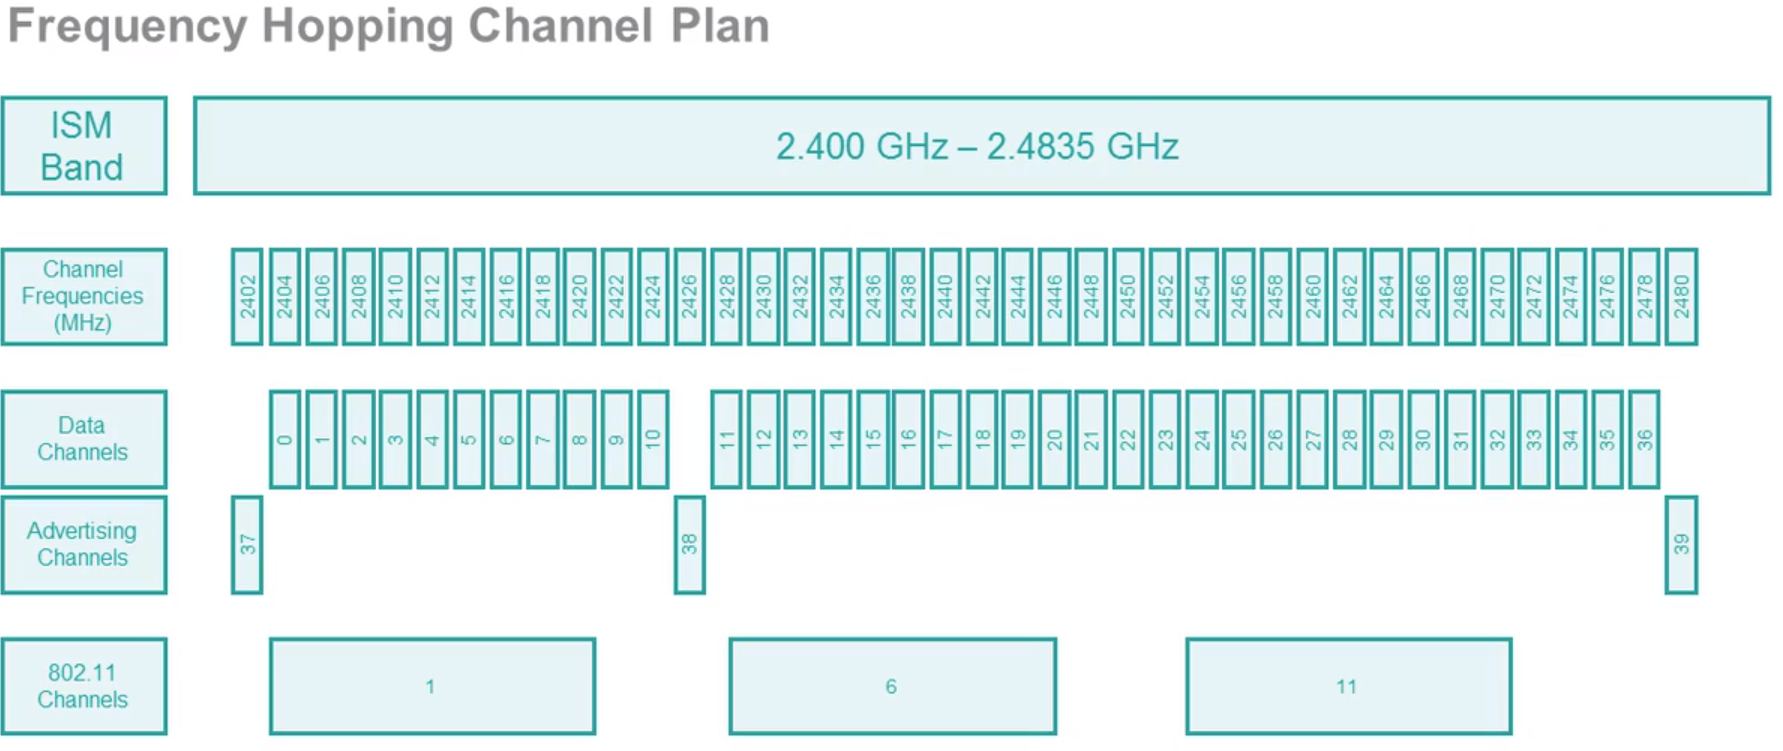
\includegraphics[width=1.0\textwidth]{Figures/Protocols/Bluetooth/ble_channels_vs_802_11.PNG}
    \caption{Bande ISM utilisée par le Bluetooth Low Energy}
    \label{fig-ble_channels_vs_802}
\end{figure}

Le Bluetooth Low Energy utilise la modulation Gaussian Frequency Shift Keying \footnote{\url{https://en.wikipedia.org/wiki/Frequency-shift_keying\#Gaussian_frequency-shift_keying}} (GFSK).  La différence entre le Bluetooth Low Energy et le Bluetooth Classic réside dans l'index de la modulation qui s'élève à 0.35 pour le \textit{Classic} et 0.5 pour le Low Energy \cite{BluetootModulation:online}.

\subsection{Interopérabilité entre les dispositifs}

La \cref{sec-stateoftheart_ble} explore la différence entre le Bluetooth et le Bluetooth Low Energy, mais il faut savoir que certains problèmes d'incompatibilité persistent entre les deux technologies. En réalité, il existe deux mondes. Le premier est celui du Bluetooth \textit{standard} ou \textit{classic}, les dispositifs communiquant dans ce monde sont labellisés \textit{Bluetooth}. Le deuxième monde est celui des dispositifs communiquant en Low Energy, ces dispositifs ont le label \textit{Bluetooth Smart}. Ces derniers ne peuvent pas communiquer avec les premiers et vice-versa. La communication entre les deux mondes est réservée aux dispositifs de type \textit{Bluetooth Smart Ready}. De moins en moins de dispositifs ne sont labellisés que Bluetooth, mais il existe encore de vieux appareils qui ne sont pas \textit{Smart Ready}. De nos jours, tous les smartphones sont \textit{Smart Ready}. La communication entre ces deux mondes est visible sur la \cref{fig-bluetooth_interoperabilty}.



\begin{figure}[ht!]
    \centering
    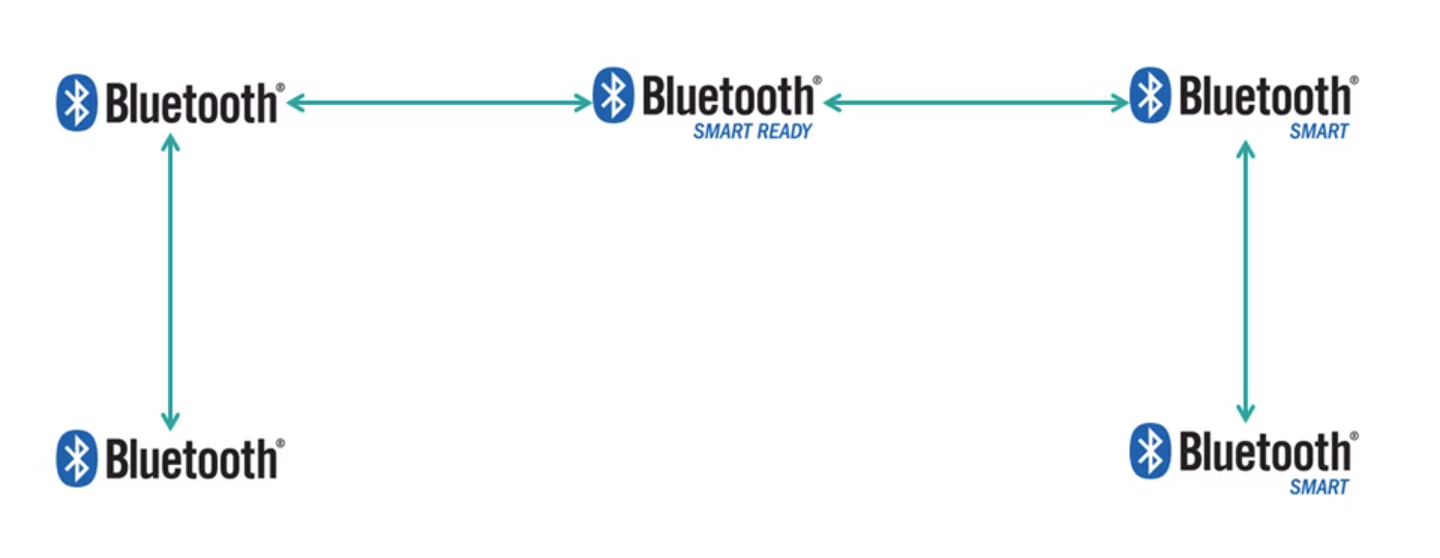
\includegraphics[width=0.7\textwidth]{Figures/Protocols/Bluetooth/bluetooth_interoperabilty.PNG}
    \caption{Interopérabilité entre les dispositifs Bluetooth}
    \label{fig-bluetooth_interoperabilty}
\end{figure}


\subsection{Rôles}
\label{sec-protocol_ble_roles}


En Bluetooth Low Energy, quatre terminologies décrivent les objets souhaitant établir une connexion Bluetooth et échanger des informations une fois connectés. La \cref{fig-central_vs_peripheral} illustre ces quatre terminologies. En premier lieu, il y a les objets en eux même, soit sur l'illustration un capteur de fréquence cardiaque. Ensuite, un smartphone ou PC qui souhaite récupérer les données ce cet objet. Un dispositif qui souhaite engager la connexion porte le nom de \textbf{centrale}. Le dispositif acceptant la connexion est quant à lui nommé \textbf{périphérique}. Une fois la connexion établie, il est possible d'échanger des données. Là, les noms ne sont plus les mêmes, car c'est maintenant le rôle des services Bluetooth de fournir les données (cf. \cref{sec-protocols_BLE_services}). La centrale est nommée \textbf{client}, tandis que le périphérique est le \textbf{serveur}. Les dispositifs Bluetooth sont tous identifiés à l'aide d'une adresse MAC\footnote{\url{https://en.wikipedia.org/wiki/MAC_address}} unique sur 48 bits envoyée dans tous les paquets, y compris lorsqu'une connexion doit être établie. \\

\begin{figure}[ht!]
    \centering
    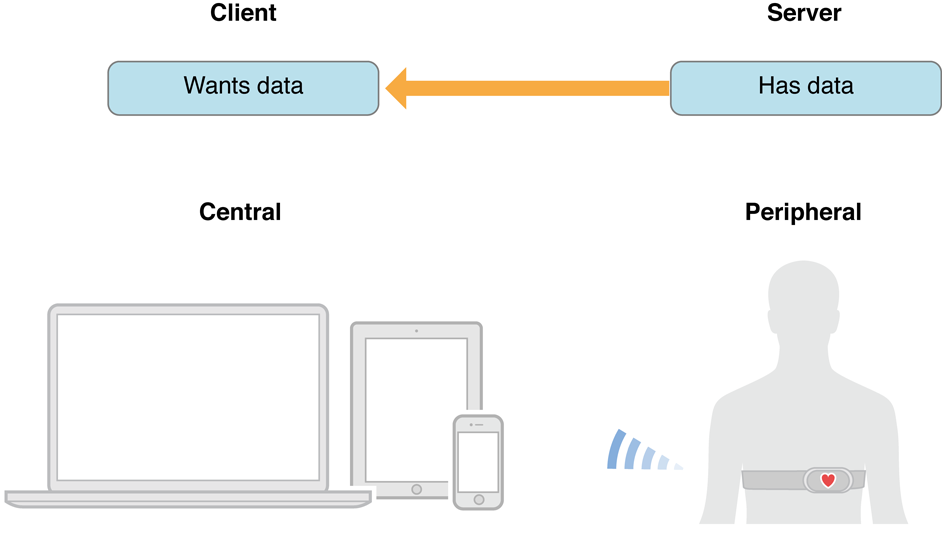
\includegraphics[width=0.7\textwidth]{Figures/Protocols/Bluetooth/central_vs_peripheral.png}
    \caption{Terminologies des connexions et des échanges de données en Bluetooth Low Energy}
    \label{fig-central_vs_peripheral}
\end{figure}

Parfois les termes «central» et «périphérique» sont remplacés par les notions de \textbf{maitre} et \textbf{esclave}, car comme dans beaucoup de protocoles, le maitre initialise la connexion (ou communication) avec l'esclave.

\subsection{\textit{Advertisements}}
\label{sec-protocol_ble_adv}

Un périphérique Bluetooth Low Energy doit s'annoncer lorsqu'il est prêt pour être connecté ou simplement quand il souhaite informer ses voisins de sa présence. Lors de la présentation des canaux Bluetooth (cf. \cref{fig-ble_channels_vs_802}), on peut constater la présence de trois canaux réservés aux \textit{advertisements}. Ceux-ci ont deux rôles. Le premier est d'annoncer à une centrale que le périphérique est disponible ou non pour une connexion BLE. Le second consiste à diffuser à toutes les centrales et périphériques aux alentours un paquet de données personnalisable par l'utilisateur. Cette dernière catégorie contient le concept de \textit{beacons}, lequel est abordé dans la \cref{sec-protocols_BLE_beacons} de ce document. Le choix du canal d'\textit{advertisements} est aléatoire (parmi les trois présentés) pour chaque nouveau paquet envoyé. \\

\begin{figure}[ht!]
    \centering
    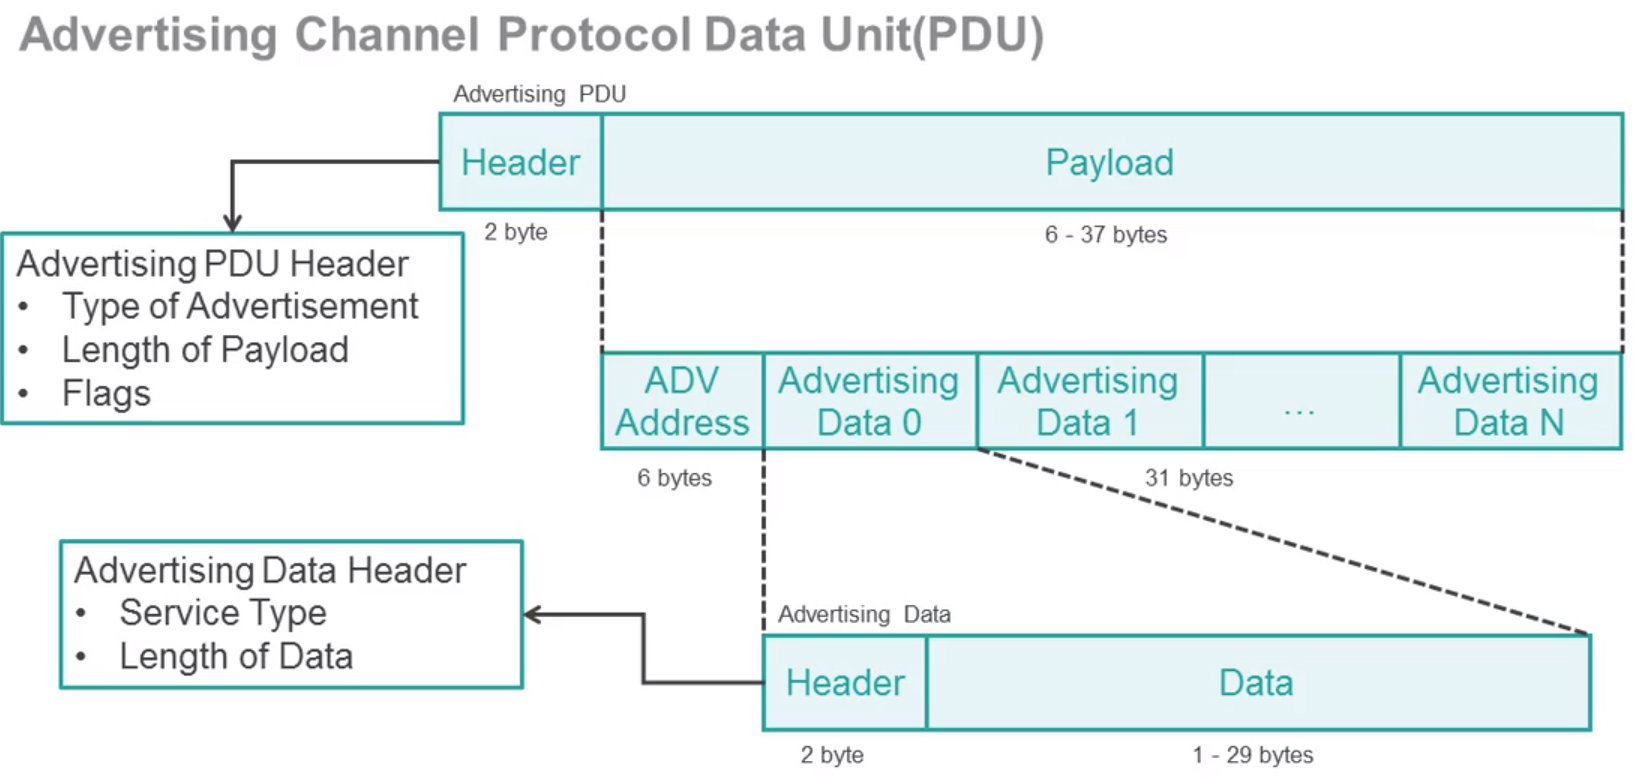
\includegraphics[width=1.0\textwidth]{Figures/Protocols/Bluetooth/ble_adv_packet_content.PNG}
    \caption{Contenu d'un paquet de type \textit{advertisement}}
    \label{fig-ble_adv_packet_content}
\end{figure}

Le contenu d'un \textit{advertisement} est illustré par la \cref{fig-ble_adv_packet_content}. La taille complète d'un \textit{advertisement} ne peut pas dépasser 39 bytes en Bluetooth 4.2. Les deux premiers bytes sont là pour renseigner les dispositifs qui scannent sur les différents paramètres et configurations offerts par le périphérique. Parmi ces informations, il est possible de savoir si le dispositif est connectable, si celui-ci utilise une adresse fixe ou variable, etc. Il indique également s’il est possible de demander au périphérique des informations supplémentaires en effectuant un \textit{Scan Request}, afin de récupérer un nouvel \textit{advertisement} contenant un \textit{Scan Response}. Pour information, le site Internet suivant offre une description très détaillée de chacun des champs et de la valeur qui peut lui être assignée : 
\begin{center}
    \small{\url{http://j2abro.blogspot.ch/2014/06/understanding-bluetooth-advertising.html}}
\end{center}

A la suite de l'entête, se trouve l'adresse MAC du périphérique (fixe ou aléatoire). S'ensuivent différents paquets de données qui sont tous accompagnés d'une nouvelle entête. C'est avec ces derniers qu'il est possible d'implémenter des \textit{beacons} (cf. \cref{sec-protocols_BLE_beacons}).\\

L'intervalle entre les \textit{advertisements} est configurable par le programmeur. Cet intervalle est normalisé et peut varier de 20\,ms à 10.24\,s avec des pas de 0.625\,ms \cite{Lesson3I56:online}. Plus cet intervalle est court, plus la centrale aura de chances de détecter le périphérique. Cependant, cette vitesse se fait au détriment de la consommation énergétique qui sera donc plus importante. L'intervalle inclut un facteur aléatoire dans le temps afin d'éviter les chances de collisions, par exemple, lorsque deux dispositifs avec le même intervalle commencent à émettre des \textit{advertisements} en même temps.

\subsection{Machine des états de la connexion}

\begin{figure}[ht!]
    \centering
    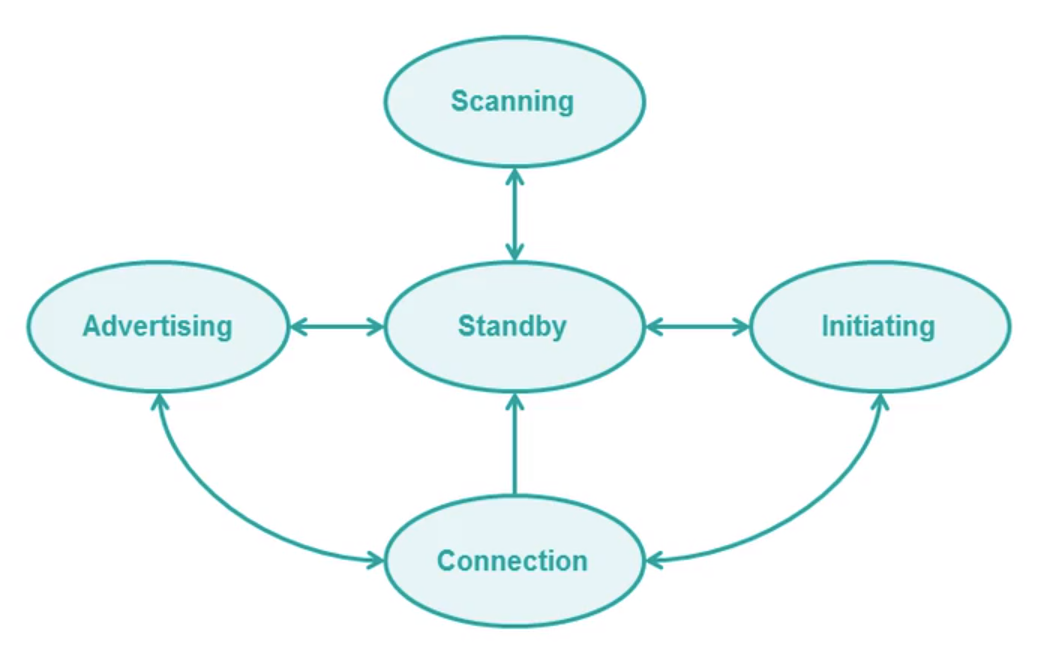
\includegraphics[width=0.8\textwidth]{Figures/Protocols/Bluetooth/state_machine_5_states.PNG}
    \caption{Les 5 états possibles pour un dispositif Bluetooth Low Energy}
    \label{fig-state_machine_5_states}
\end{figure}


Il existe 5 états possibles pour un appareil avec du Bluetooth Low Energy. Ces 5 états sont illustrés sur la \cref{fig-state_machine_5_states}, de même que les liaisons possibles entre ceux-ci. L'explication de ces états est la suivante : 

\begin{enumerate}
    \item \texttt{\textit{Standby}} : état par défaut. C'est dans ce mode que les dispositifs attendent qu'une nouvelle action leur soit demandée. C'est l'état où ils consomment également le moins d'énergie.
    \item \texttt{\textit{Advertising}} : état où le périphérique envoie des \textit{advertisements}, afin de notifier s'il est connectable ou simplement lorsqu'un dispositif souhaite envoyer des données (par exemple des \textit{beacons}).
    \item \texttt{\textit{Scanning}} : état où la centrale scanne ses environs afin de rechercher le dispositif auquel elle souhaite se connecter. Ce mode vise également la situation où la centrale est simplement intéressée par les paquets d'\textit{advertisements} qui transitent, sans forcément vouloir établir une connexion.
    \item \texttt{\textit{Initiating}} : état où la centrale décide de se connecter avec un périphérique. Elle tente de l'atteindre afin d'effectuer une procédure de connexion.
    \item \texttt{\textit{Connection}} : état où les deux périphériques ont acceptés la connexion et peuvent maintenant commencer à s'échanger des données.
\end{enumerate}

\begin{figure}[ht!]
    \centering
    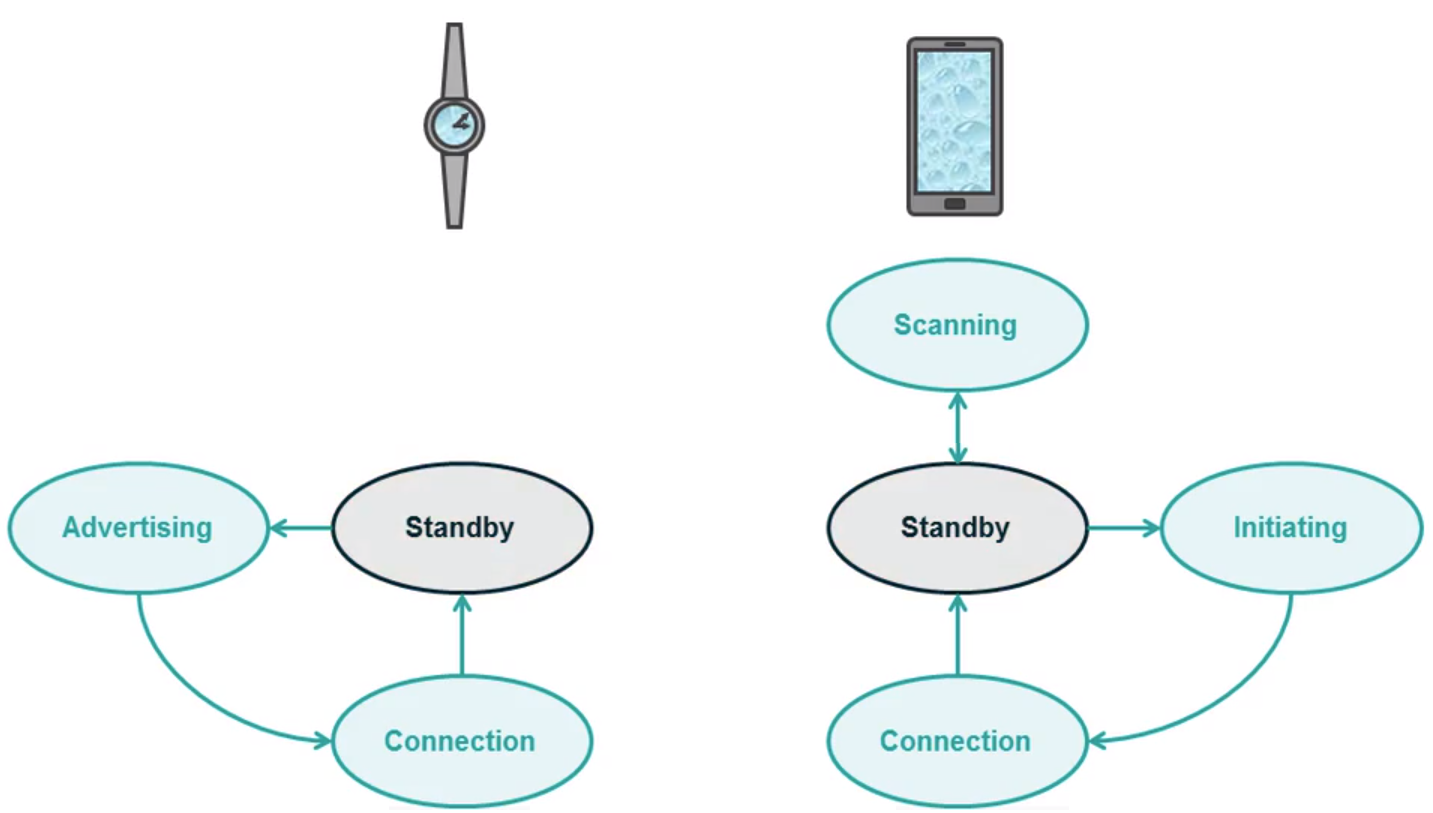
\includegraphics[width=0.8\textwidth]{Figures/Protocols/Bluetooth/states_while_connecting.PNG}
    \caption{Étapes lors de la connexion Bluetooth entre une centrale et un périphérique}
    \label{fig-states_while_connecting}
\end{figure}

Ces 5 états ne sont pas utilisés en parallèle. Un périphérique et une centrale n'en utilisent qu'un nombre limité. La \cref{fig-states_while_connecting} illustre la connexion d'un smartphone en mode central à une montre connectée en tant que périphérique. Voici la séquence de connexion de ces deux dispositifs : 

\begin{enumerate}
    \item Prenons l'exemple où les deux dispositifs commencent en mode \texttt{\textit{Standby}}.
    \item Le périphérique se met en mode \texttt{\textit{Advertising}} lorsqu'il est prêt à être connecté. En parallèle, le smartphone (centrale) se met en mode \texttt{\textit{Scanning}} pour détecter la présence du périphérique périodiquement. 
    \item Lorsque le scanne est fini, la centrale repasse en \texttt{\textit{Standby}}. Si dans ce mode celle-ci détecte la présence de son périphérique via les données reçues de l'état \texttt{\textit{Scanning}}, celle-ci entre en mode \texttt{\textit{Initiating}} afin d'initier une procédure de connexion avec le périphérique.
    \item Si le périphérique accepte la connexion provenant de la centrale, les deux passent alors dans l'état \texttt{\textit{Connection}}. Si la connexion échoue, les deux dispositifs repassent en \texttt{\textit{Standby}}. Le périphérique peut se remettre à générer des \textit{advertisements} s'il le souhaite.
\end{enumerate}


\subsection{Architecture d'une \textit{stack} Bluetooth}

\begin{figure}[ht!]
    \centering
    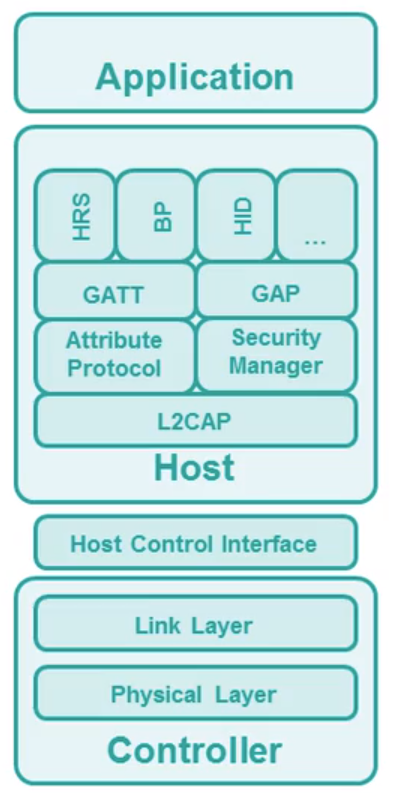
\includegraphics[width=0.3\textwidth]{Figures/Protocols/Bluetooth/ble_full_stack_explained.PNG}
    \caption{Architecture complète de la stack BLE}
    \label{fig-ble_full_stack_explained}
\end{figure}

L'architecture Bluetooth se subdivise en trois dénominations principales, illustrées à la \cref{fig-ble_full_stack_explained}. Ces trois subdivisions se nomment \texttt{Controller}, \texttt{Host} et \texttt{Application}. Entre le \texttt{Controller} et l'\texttt{Host}, il existe un quatrième élément d'interfaçage nommé \textit{Host Control Interface}. Le but de cette sous-section est d'explorer les différents composants de chacune de ces dénominations, afin d'avoir une vue plus complète du protocole Bluetooth Low Energy. Une partie de ces explications proviennent de la vidéo nommée \textit{Lesson 3: Introduction to Bluetooth Low Energy}\footnote{\url{https://www.nxp.com/video/lesson-3-introduction-to-bluetooth-low-energy:LESSON-3-KW41Z-WIRELESS-LAB}} par NXP. 

Dans un OS, ces trois tâches consistent souvent en trois processus bien distincts qui communiquent entre elles avec des interfaces tenant compte des problèmes liés à la concurrence. Il est important de comprendre comment ces trois entités fonctionnent lorsque l'on programme sur un dispositif aussi bas niveau qu'un microcontrôleur. 


\subsubsection{\textit{Controller}}

Le contrôleur est la brique la plus basse du Bluetooth et a pour but de gérer l'interface RF avec les différentes spécificités liées à celle-ci. Elle est dépendante de l'implémentation matérielle du dispositif. Cette interface est différente pour chaque contrôleur utilisé, mais implémente des concepts similaires.

\subsubsubsection{\textit{Physical Layer}}

La couche physique s'occupe de toute la gestion des différents canaux présentés précédemment sur la \cref{fig-ble_channels_vs_802}. Cette couche effectue les décalages en fréquences (\textit{Frequency Hopping Spread Spectrum}), mais ce n'est pas elle qui choisit les \textit{timings} des sauts de fréquences. Son rôle est uniquement de générer la modulation demandée par la couche supérieure, avec les paramètres qui lui sont appliqués.

\subsubsubsection{\textit{Link Layer}}

La couche \texttt{Link Layer} se charge de la gestion des connexions ainsi que de la qualité de celles-ci. Cette couche communique avec la \texttt{Physical Layer} lorsque le \textit{Frequency Hopping Spread Spectrum} doit être adapté en raison d'une saturation du réseau. Cette couche gère également tous les aspects des connexions Bluetooth Low Energy.


\subsubsection{\textit{Host Control Interface}}

Le \texttt{Host Control Interface}, souvent abrégé par \textit{HCI}, est une interface standardisée entre l'Host et le Controller. Cette interface implémente les mêmes concepts, quelleque soit la plateforme. L'avantage de cd type d'interface est de gagner du temps lorsque l'on change de contrôleur RF. Ainsi, seule la brique inférieure doit être modifiée sans influencer celles du dessus. L'interface HCI est également présente dans le Bluetooth \textit{standard}. La base est similaire (entre les deux), mais les \textit{advertisements} et les scans nécessitent de nouvelles commandes. \\

Dans certaines implémentations, le contrôleur est un périphérique externe au microcontrôleur et est connecté à celui-ci à l'aide d'une interface série (UART, SPI, etc.). Aussi, on retrouve le HCI dans ce type d'utilisations, bien que celle-ci soit du côté périphérique et convertisse ensuite les données en série en un format standardisé HCI.

\subsubsection{\textit{Host}}


L'\textit{Host} est l'élément le plus complexe du Bluetooth. Le but de cette section n'est pas d'explorer toutes les spécificités de cet élément, mais de comprendre ses rôles et ses composants principaux.



\subsubsubsection{\textit{L2CAP}}

L2CAP signifie \texttt{Logical link control and adaptation protocol}. Il a les fonctions suivantes : 
\begin{enumerate}
    \item Transporter les données pour les couches de niveau supérieures, avec la gestion du \textit{multiplexing} sur un même lien de données;
    \item Segmenter et réassembler les paquets de données;
    \item Concentrer les données provenant de plusieurs flux en une seule interface;
    \item Gérer la \textit{Quality of Service} pour les couches supérieures. Il s'occupe de la gestion des erreurs et retransmet des données si celles-ci échouent.
\end{enumerate}


\subsubsubsection{\textit{GAP}}
\label{sec-protocols_BLE_GAP}

GAP signifie \texttt{Generic Access Profile}. Il s'agit d'un service Bluetooth Low Energy qui vise à configurer l'accessibilité du périphérique. On trouve les informations suivantes dans ce service : 
\begin{enumerate}
    \item le périphérique peut-t-il être découvert et comment le découvrir;
    \item le périphérique est-il connectable et quelles sont les configurations nécessaires pour mettre en place cette connexion si elle est acceptée.
    \item le périphérique est-il \textit{bondable} (cet aspect sera exploré plus en détail avec la thématique de la sécurité Bluetooth Low Energy de la \cref{sec-security_ble}). 
    \item Une fois le \textit{bond} effectué, le GAP s'occupe de la gestion des clés de sécurité et de l'autorisation des centrales qui peuvent se connecter au périphérique.
\end{enumerate}

Le service GAP définit également les rôles implémentés par le dispositif. Les deux rôles "centrale" et "périphérique" ont été présentés précédemment, mais il existe deux \textit{sous-rôles} : 
 
\begin{enumerate}
    \item \texttt{Broadcaster} : principe appliqué par les dispositifs de type \textit{beacons} (cf. \cref{sec-protocols_BLE_beacons}), c'est un périphérique qui émet des \textit{advertisements,} mais qui n'est jamais connectable.
    \item \texttt{Observer} : scanneur qui scrute en permanence le réseau Bluetooth Low Energy, mais qui n'initie pas de connexion avec un périphérique.
\end{enumerate}

\subsubsubsection{\textit{Security Manager}}
\label{sec-protocols_BLE_security_manager}

Le \texttt{Security Manager} porte, comme son nom l'indique, sur la gestion de tout l'aspect sécurité du périphérique. Il génère les clés lors des différentes connexions. Les clés temporaires sont stockées pour la session active, tandis que des \textit{Long Term Key} (LTK) sont utilisées pour les périphériques \textit{bonded} (cf. \cref{sec-security_ble} pour plus de détails). Ce bloc s'occupe également de chiffrer les données lorsque le type de sécurité appliqué le demande.


\subsubsubsection{\textit{ATT}}

ATT signifie \texttt{Attribute Protocol}. Ce bloc crée les deux interfaces Serveur et Client (cf. \cref{sec-protocol_ble_roles}). Les éléments effectuant la mise à disposition de ces données sont appelés \textit{Attributes} et présentent les caractéristiques suivantes : 
\begin{itemize}
    \item \texttt{Attribute Type} : Un attribut est défini par un identifiant unique. Celui-ci est un UUID\footnote{\url{https://en.wikipedia.org/wiki/Universally_unique_identifier}} sur 128-bit. Cet identifiant peut être raccourci à 16 bits, lorsqu'il s'agit d'identifiants standardisés Bluetooth.
    \item \texttt{Attribute Handle} : définit où l'attribut est sauvegardé sur le serveur.
    \item \texttt{Attribute Value} : comme son nom l'indique, cette caractéristique définit la valeur de l'attribut. La taille maximale assignable à celui-ci est de 512 bytes.
    \item \texttt{Attribute Permissions} : Les permissions définissent les différentes opérations pouvant être effectuées sur l'attribut. Par exemple, \textit{Read}, \textit{Write} ou \textit{Read/Write} simultanément.
\end{itemize}

\begin{figure}[ht!]
\centering
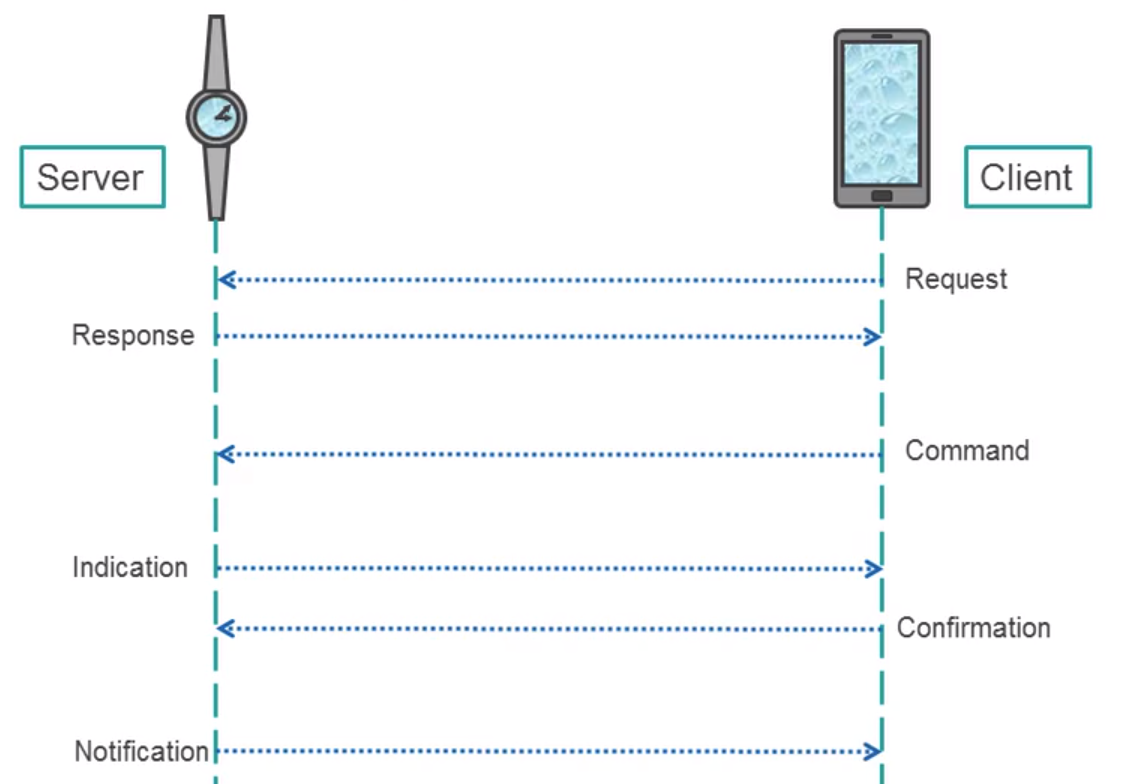
\includegraphics[width=0.8\textwidth]{Figures/Protocols/Bluetooth/client_server_4_operations.png}
\caption{Opérations possibles entre un serveur et un client Bluetooth Low Energy}
\label{fig-client_server_4_operations}
\end{figure}


Une fois connecté, l'accès à un attribut entre un serveur et un client peut s'effectuer à l'aide de quatre opérations. Ces opérations, décrites sur la \cref{fig-client_server_4_operations}, sont les suivantes :
\begin{enumerate}
    \item \texttt{Request/Response} : Lorsque le client souhaite uniquement \underline{lire} un attribut depuis le serveur, il effectue une opération de type \textit{request}. Le serveur lui répond ensuite avec une \textit{response}. 
    \item \texttt{Command} : Lorsque le client souhaite \underline{écrire} un attribut, il effectue une opération de type \textit{command}. Il existe une variante de la commande où il est possible de rajouter une confirmation lors de l'écriture.
    \item \texttt{Indication} : Lorsque le serveur a une nouvelle donnée disponible sur l'attribut, il peut l'envoyer au client sous forme d'\texttt{indication}. Si le client récupère correctement cette donnée, un accusé de réception est envoyé \underline{avec une confirmation} au serveur.
    \item \texttt{Notification} : Lorsque le serveur a une nouvelle donnée disponible sur l'attribut, il peut l'envoyer au client sous forme de notification. Cependant, contrairement à l'indication, la réception de donnée par le client \underline{n'est pas confirmée}. Cela permet ainsi d'économiser des échanges et d'augmenter le débit ou de réduire la consommation. 
\end{enumerate}

\subsubsubsection{\textit{GATT}}

GATT signifie \texttt{Generic Attribute Profile}. C'est une couche au-dessus de l’ATT qui a pour but de hiérarchiser les différents groupes d'attributs en un concept nommé \texttt{\textbf{Services Bluetooth Low Energy}}. 

Le GATT gère également la découverte de ces divers services en répondant aux requêtes de type \texttt{Discovery Services} d'un client. Le format pour la découverte est doté de diverses règles qui sont appliquées par le GATT.


\subsubsubsection{\textit{Profils et services}}
\label{sec-protocols_BLE_services}

Sur la \cref{fig-ble_full_stack_explained} on peut remarquer la présence de plusieurs blocs au-dessus du GATT. Il s'agit là de services GATT standardisés. Trois services sont listés : 
 \begin{itemize}
     \item \texttt{HRS} : signifie \textit{Heart Rate Service}
     \item \texttt{BP} : signifie \textit{Blood Pressure Service}
     \item \texttt{HID} : signifie \textit{Human Interface Device Service}, lequel offre ainsi la possibilité de connecter des périphériques à l'aide du Bluetooth Low Energy (ex. souris sans fil)
 \end{itemize}


Ces services sont intégrés dans des \textbf{profils} standardisés par le protocole Bluetooth : 
\begin{center}
    \url{https://www.bluetooth.com/specifications/gatt}
\end{center}

Le but de ces profils standardisés est d'augmenter l'interopérabilité des différents appareils avec les interfaces de données standards. Par exemple, dans le cas d'un HRS, l'interface de capture du système cardiaque est standard, ce qui permet à n'importe quel développeur de faire une application générique pour tous les capteurs cardiaques du marché. \\

Si un développeur souhaite créer son propre profil, il doit se plier à certaines restrictions quelques restrictions. Les UUIDs des attributs ne peuvent pas utiliser l'UUID attribué aux services Bluetooth standardisés, à savoir la valeur \path{0000XXXX-0000-1000-8000-00805f9b34fb}. Les \texttt{XXXX} représentent le UUID 16 bits pouvant être utilisés au lieu des 128 bits, lorsque les services standards sont accédés. La liste complète de ces services, ainsi que leur UUID 16bit, est disponible à l'adresse suivante : 
\begin{center}
    \url{https://www.bluetooth.com/specifications/gatt/services}
\end{center}



\begin{table}[ht!]
\centering
\caption{Paramètres d'un \textit{Client Characteristic Configuration Descriptor}}
\label{tab-cccd_parameters}
\begin{tabular}{|l|l|l|l|}
\hline
\multicolumn{4}{|l|}{\cellcolor[HTML]{BBDAFF}{\color[HTML]{333333} \textbf{Bit Field Client Characteristic Configuration (CCCD)}}} \\ \hline
                                      &                                       & \multicolumn{2}{l|}{\textbf{Definition}}           \\ \cline{3-4} 
\multirow{-2}{*}{\textbf{Bit}}        & \multirow{-2}{*}{\textbf{Size}}       & \textbf{Key}       & \textbf{Value}                \\ \hline
                                      &                                       & 0                  & Notifications disabled        \\ \cline{3-4} 
\multirow{-2}{*}{0}                   & \multirow{-2}{*}{1}                   & 1                  & Notifications enabled         \\ \hline
                                      &                                       & 0                  & Indications disabled          \\ \cline{3-4} 
\multirow{-2}{*}{1}                   & \multirow{-2}{*}{1}                   & 1                  & Indications enabled           \\ \hline
                                      &                                       & 0                  & Reserved for future use       \\ \cline{3-4} 
\multirow{-2}{*}{2 to 15}             & \multirow{-2}{*}{14}                  & 1                  & Reserved for future use       \\ \hline
\end{tabular}
\end{table}


La couche ATT indique que tout élément avec un UUID est un attribut. Au niveau GATT, on utilise toutefois des définitions différentes pour chaque élément. Un \textbf{service} ne produit pas de données, son unique rôle étant de définir une encapsulation pour des \textbf{caractéristiques}. Ce sont les caractéristiques qui contiennent toutes les données des capteurs. Une caractéristique peut ensuite être accompagnée de plusieurs \textbf{descripteurs}\footnote{\url{https://www.bluetooth.com/specifications/gatt/descriptors}}. Les descripteurs ont pour rôle de configurer ou simplement d'informer une caractéristique. Le descripteur le plus connu et utilisé est le \texttt{Client Characteristic Configuration Descriptor} (CCCD). Si une caractéristique est autorisée à envoyer ses données en tant que notifications ou indications, l'utilisateur doit configurer ce descripteur pour activer ces fonctionnalités. Les paramètres possibles de ce descripteur sont visibles sur la \cref{tab-cccd_parameters}. 


\begin{figure}[ht!]
\centering
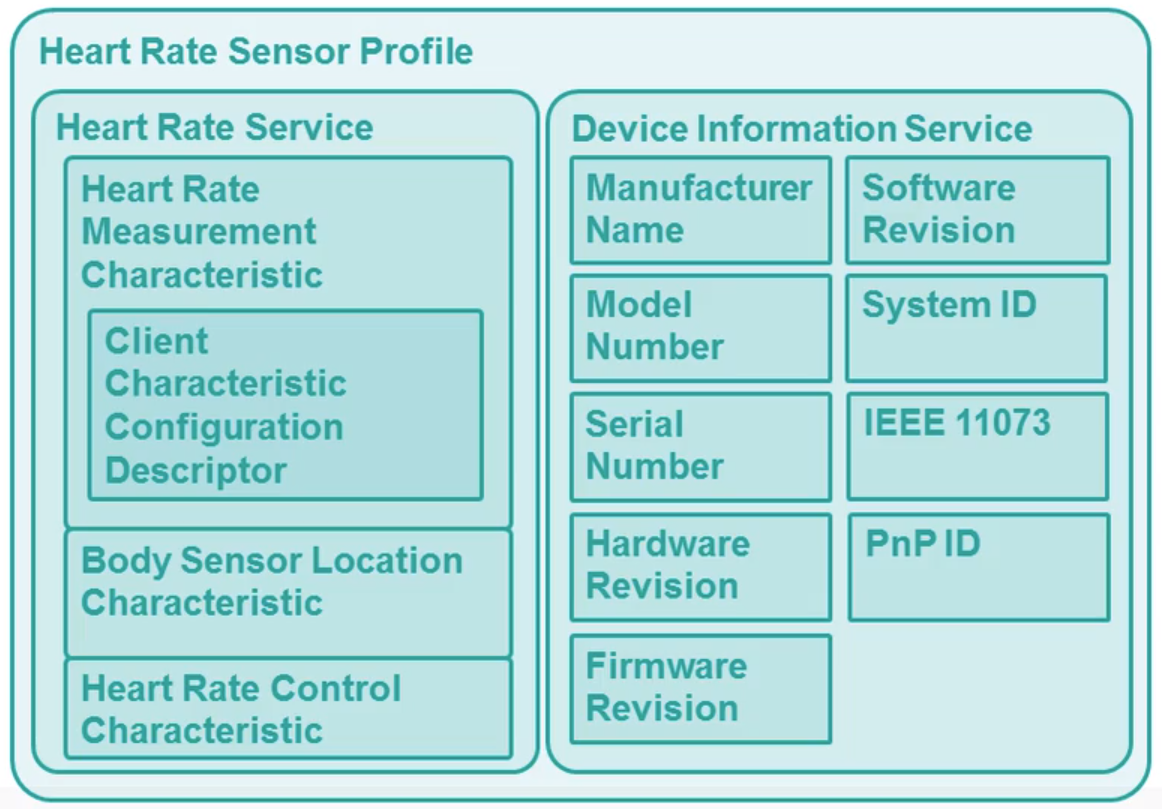
\includegraphics[width=0.6\textwidth]{Figures/Protocols/Bluetooth/heart_rate_sensor_profile.png}
\caption{Profil \textit{Heart Rate Sensor} standardisé}
\label{fig-heart_rate_sensor_profile}
\end{figure}

Lorsqu'un développeur crée un profil, il doit parfaitement comprendre ses couches intérieures afin que son implémentation soit correcte. Si on reprend l'exemple du \textit{HRS}, dont les éléments sont visibles sur la \cref{fig-heart_rate_sensor_profile}, on y voit le contenu complet qui doit être implémenté pour qu'un dispositif soit compatible avec ce profil. On a tout d'abord deux services, le principal étant celui de la mesure cardiaque. Le deuxième est le \texttt{Device Information Service}, qui comme son nom l'indique, fournit des informations sur le périphérique. Il y a ensuite la présence de trois caractéristiques : la \texttt{Heart Rate Control} permet de configurer le temps entre chaque nouvelle acquisition de valeur; La \texttt{Body Sensor Location}, qui informe sur l'emplacement du corps où le périphérique est situé; la \texttt{Heart Rase Measurement}, caractéristique la plus importante qui fournit la fréquence capturée par le capteur cardiaque. Cette caractéristique est disponible en tant que notification ou indication, puisqu'elle est également constituée d'un CCCD. Si deux profils demandent l'implémentation du même serveur, par exemple le \texttt{Device Information Service}, celui-ci n'a besoin d'être implémenté qu'une seule fois.


\subsubsection{\textit{Application}}

L'application est là où toutes les données des services sont acquisitionnées. Les communications avec les capteurs sont effectuées à ce niveau, puis une fois les données récupérées, elles sont inscrites dans les attributs ATT correspondants, à travers la base de données GATT.


\subsection{Beacons}
\label{sec-protocols_BLE_beacons}

En principe, il est possible de savoir combien de dispositifs sont présents simplement en effectuant un scan. Si l'utilisateur a son Bluetooth activé, le système va périodiquement scanner ses environs et communiquer son adresse MAC lors des réponses aux \textit{Scan Requests}. Cependant, depuis la norme 4.0 du Bluetooth Low Energy (améliorés avec la norme 4.2\cite{Bluetoot24:online}), les périphériques doivent supporter le principe de Low Energy (LE) Privacy\cite{Bluetoot24:online}. Il ne doit pas forcément être activé par défaut, mais cette option doit être implémentée sur tous les contrôleurs Bluetooth 4.2. Ce mode a pour but de modifier périodiquement l'adresse MAC du périphérique lorsque celui-ci envoi des \textit{advertisements}. Cela a pour effet d'empêcher la traque de personnes à leur insu, au moyen d'une simple borne qui scan tous les périphériques à proximité. Le microcontrôleur KW41Z supporte ce mode, comme tous les smartphones iOS ou Android. Le but étant de scanner le nombre de personnes autour d'une borne, il faut pouvoir détecter ces personnes par un moyen sûr. Les systèmes d'exploitation des smartphones (iOS et Android) ont activé par défaut le mode privacy sans possibilité de le désactiver pour les programmeurs. La fréquence du changement d'adresse MAC enduite par le LE Privacy est de l'ordre de 3min sur un smartphone, mais celle-ci varie selon les modèles de \textit{smartphones} et n'est pas configurable par le développeur. \\

Pour pallier à cette limitation, le principe de \textit{beacons} s'est très vite répandu. Il s'agit alors de modifier le contenu d'un paquet \textit{advertisement} afin d'y placer un \textit{payload} personnalisable. La transmission d'un \textit{beacon} est unidirectionnelle. Le périphérique qui scanne les \textit{beacons} ne peut pas directement interagir avec eux. Normalement, le scanner a uniquement besoin de connaitre les périphériques qui l'entoure, ainsi que la distance qui les sépare (calculable avec la puissance du signal RSSI). Les \textit{beacons} ont tous une taille de paquet maximale de 31 bytes (cf. \cref{sec-protocol_ble_adv}), dont trois bytes réservés au champ \textit{Advertisement Flag} (Adv Flag) obligatoire.

Il existe trois spécifications de \textit{beacons} principalement utilisées \cite{Understa87:online} : 

\begin{enumerate}

\begin{figure}[ht!]
\centering
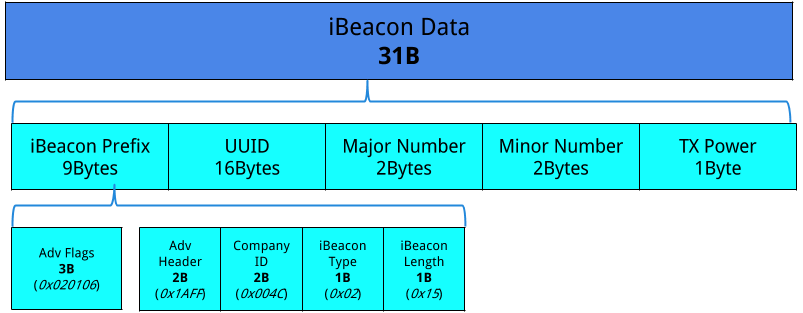
\includegraphics[width=0.8\textwidth]{Figures/Protocols/Bluetooth/ibeacon-spec-exploded-view.png}
\caption{Spécification des paquets iBeacons}
\label{fig-ibeacon-spec-exploded-view}
\end{figure}

    \item iBeacons : spécification de protocole développé par Apple\footnote{\url{https://developer.apple.com/ibeacon/}}. Le contenu du paquet BLE est affiché sur la \cref{fig-ibeacon-spec-exploded-view}. Le paquet contient un entête constitué d'un \textit{Company ID}, lequel doit être délivré par Apple pour chaque fabricant de \textit{beacons} afin que celui-ci soit conforme à la spécification. On a ensuite un UUID, unique pour chaque \textit{beacon}, \textit{Major} qui identifie un sous-réseau de plusieurs \textit{beacons} et un \textit{Minor} qui identifie un \textit{beacon} précis. L'utilisateur peut ensuite utiliser ces trois identifiants pour récupérer les informations sur le \textit{beacon} dans une base de données. En fin du paquet, il y a la puissance d'émission en dBm à 1m afin d'estimer la distance en fonction du RSSI mesuré par le scanneur. Le paquet fait au total 31 bytes, mais uniquement 20 bytes (UUID, \textit{Major} et \textit{Minor}) sont configurables par l'utilisateur, le reste étant fixé par Apple ou le fabricant certifié du \textit{beacon}.
    

\begin{figure}[ht!]
\centering
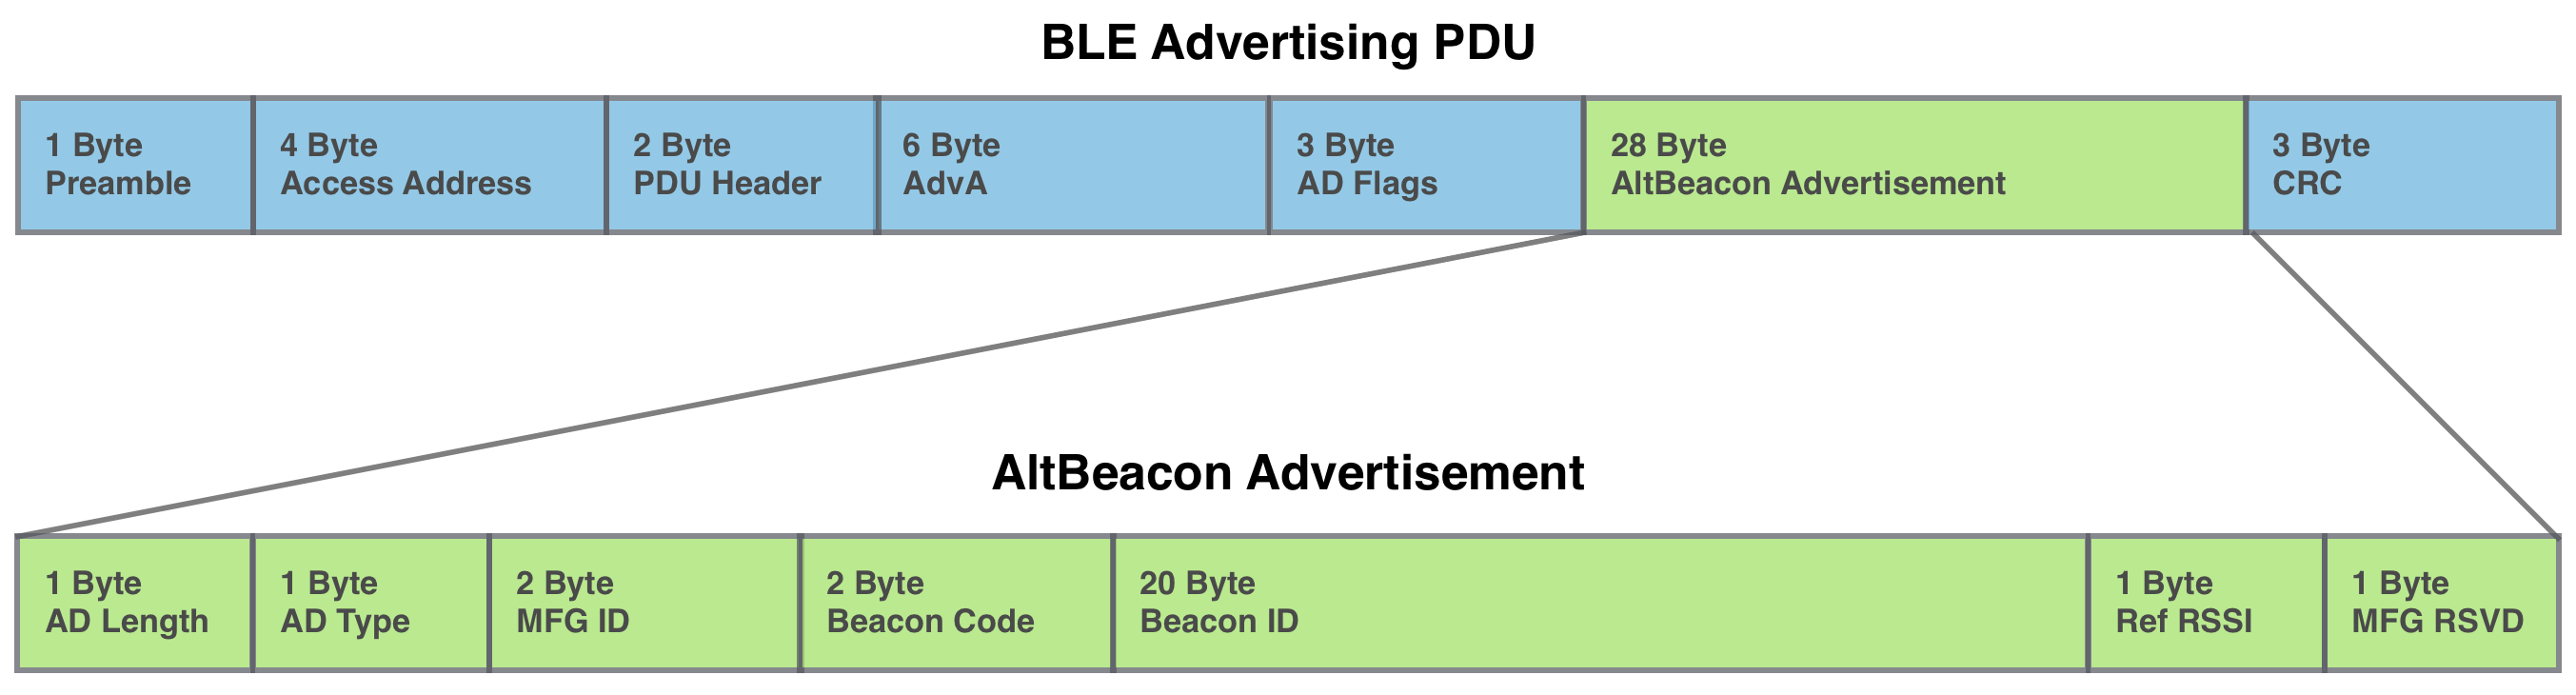
\includegraphics[width=1.0\textwidth]{Figures/Protocols/Bluetooth/altbeacon-spec-exploded-view.png}
\caption{Spécification des paquets AltBeacon}
\label{fig-altbeacon-spec-exploded-view}
\end{figure}

    \item AltBeacon : spécification de protocole développé par Radius Networks \footnote{\url{http://altbeacon.org/}}. Le contenu du paquet BLE est affiché sur la \cref{fig-altbeacon-spec-exploded-view}. Le contenu du champ Beacon ID est identique à l'identifiant utilisé par le iBeacon, c'est-à-dire l'utilisation d'un UUID sur 16 bytes couplé à un \textit{Major} et \textit{Minor} sur deux bytes chacun. L'AltBeacon a 25 bytes modifiables par l'utilisateur, car les champs \textit{Manufacturer ID }(MFG ID), \textit{Beacon Code} et \textit{Manufacturer Reserved Data} (MFG RSVD) sont tous configurables par l'utilisateur. 


\begin{figure}[ht!]
\centering
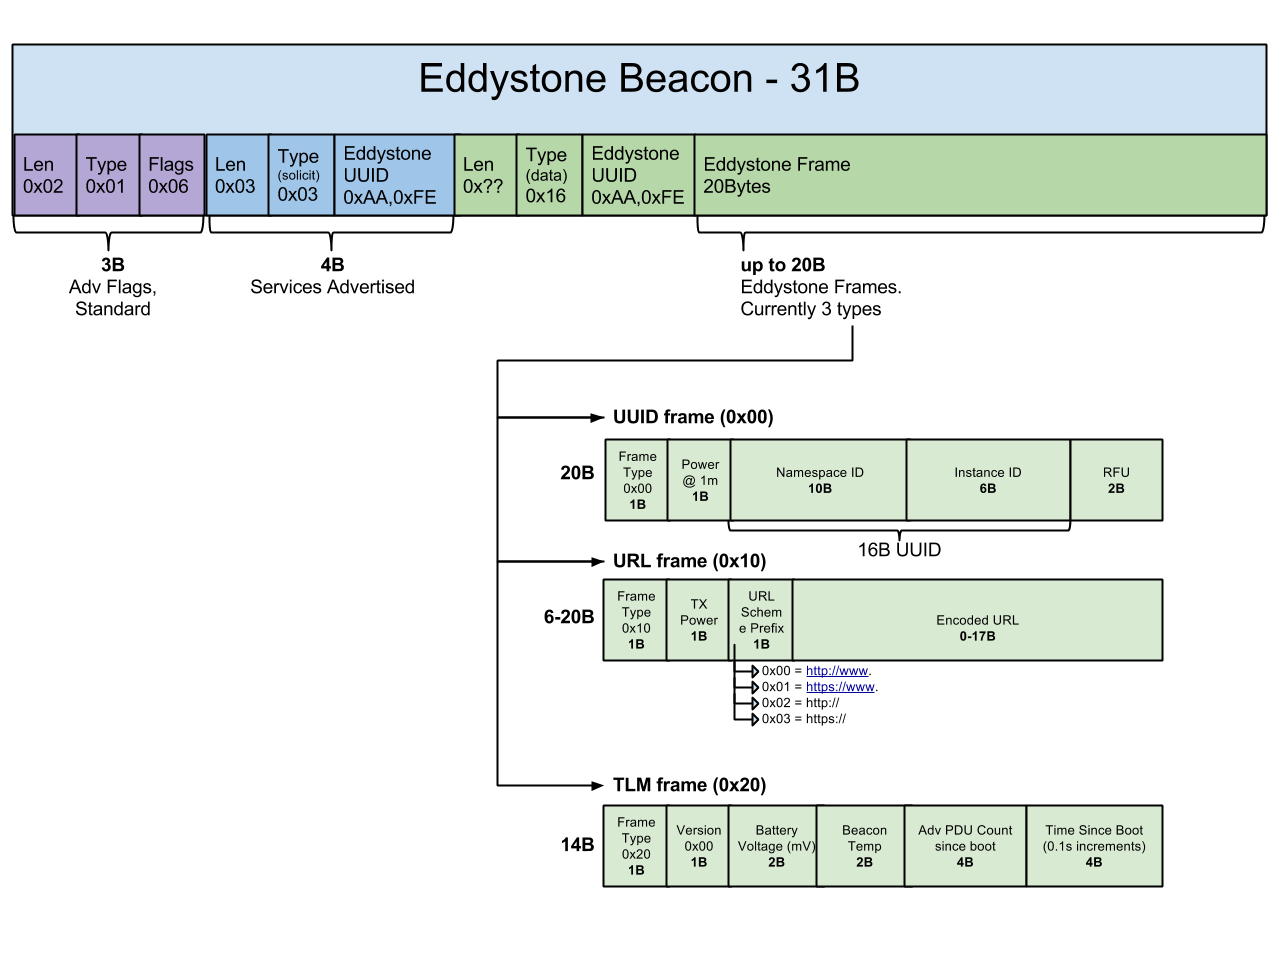
\includegraphics[width=1.0\textwidth]{Figures/Protocols/Bluetooth/eddystone-spec-exploded-view.png}
\caption{Spécification des paquets Eddystone}
\label{fig-eddystone-spec-exploded-view}
\end{figure}
    \item Eddystone : spécification de protocole développé par Google \footnote{\url{https://github.com/google/eddystone}} et initialement appelée URIBeacon. Le contenu du paquet BLE est affiché sur la \cref{fig-eddystone-spec-exploded-view}. Cette spécification a un but différent des deux autres précédemment décrites. Celle-ci fait partie de l'initiative Physical Web\footnote{\url{http://google.github.io/physical-web/}}, qui a pour objectif de faciliter l'interaction avec les objets qui entourent les utilisateurs sans nécessiter une connexion Bluetooth. Il existe trois types de paquets Eddystone :
    \begin{enumerate}
        \item \texttt{UUID} : similaire aux deux technologies précédentes, son but est de diffuser une UUID de 16 bytes découpés en deux champs de 10 et 6 bytes.
        \item \texttt{URL} : Le \textit{beacon} peut diffuser une URL qui peut être lue par un client avec un accès internet. Il peut par exemple diffuser l'URL \url{https://goo.gl/Aq18zF} et chaque client recevant ce paquet pourra visiter le site sur son téléphone. La navigateur Google Chrome sur Android offre ainsi la possibilité de scanner ses environs à la recherche de périphériques proposant des URL Eddystones.
        \item \texttt{TLM} : Offre la possibilité de diffuser des informations télémétriques sur le \textit{beacon}. On peut ainsi connaitre la batterie du périphérique, la température ainsi que le nombre d'\textit{advertisements} envoyés depuis qu'il a démarré. 
    \end{enumerate}
    La spécification UUID est la plus intéressante, mais elle reste plus limitée que le iBeacon ou l'AltBeacon. En effet, elle n'offre que 16 bytes modifiables.
\end{enumerate}



Le but principal de ces \textit{beacons} est d'informer l'utilisateur sur les événements survenant autour de lui, mais ceux-ci peuvent être détournés pour localiser les gens. En effet, si on place des \textit{beacons} fixes, on peut ensuite remonter via Internet la liste des \textit{beacons} à proximité et leurs puissances. Si un grand nombre de \textit{beacons} sont à proximité, il est donc possible de traquer une personne à quelques mètres près. Pour ce faire, une application smartphone qui scan les \textit{beacons} et qui remonte les informations à un serveur est nécessaire. Par contre, conscient de cette invasion de la privacité, les développeurs doivent maintenant demander les droits de localisation sur l'application (même principe pour iOS et Android) afin d'effectuer des scans lorsque le téléphone est en veille.

\FloatBarrier



\subsection{Consommation énergétique}


Le Bluetooth Special Interest Group (SIG) affirme que le BLE consomme entre 1 et 50\,\%, de la consommation du Bluetooth Classic \cite{BLEConsumption:online}. Ce gap oscille selon l'application souhaitée. La \cref{fig-power_consumptions_ble_advertising} illustre la consommation des périphériques en mode \textit{advertising} \cite{BLECONSUMPTIONPUBLICATION}. On constate que les facteurs qui influencent sur la consommation sont: la taille des paquets, l'intervalle entre chaque paquet et la puissance d'émission. Lorsque l'utilisateur le développeur souhaite optimiser la consommation il doit tenir compte de ses trois paramètres. Selon les systèmes utilisés, ces paramètres ne sont pas flexibles. Par exemple, sur Android, le développeur peut uniquement mettre trois modes de fréquences pour le paquet Bluetooth sans jamais pouvoir spécifier un intervalle temporel. Le temps ensuite appliqué varie selon le modèle du périphérique.

\begin{figure}[ht!]
\centering
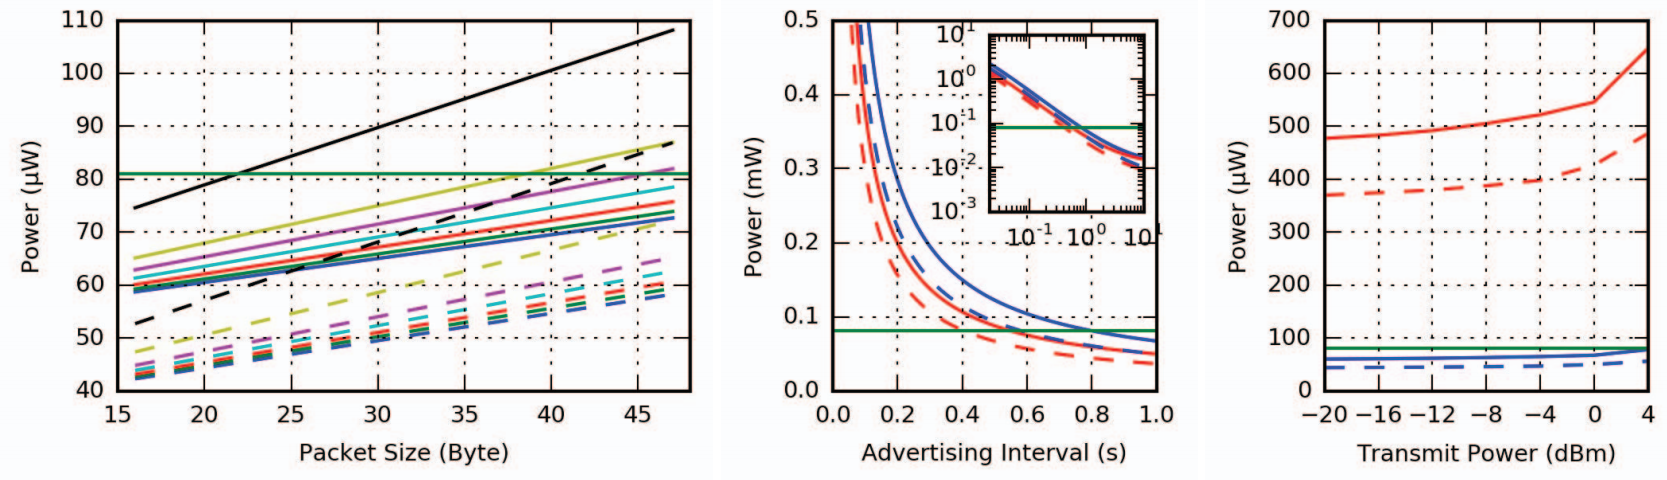
\includegraphics[width=1.0\textwidth]{Figures/Protocols/Bluetooth/power_consumptions.png}
\caption{Consommation des \textit{advertisements} en Bluetooth Low Energy}
\label{fig-power_consumptions_ble_advertising}
\end{figure}



\FloatBarrier






\section{LoRaWAN}
\label{sec-protocols_lorawan}


Le protocole LoRaWAN a brièvement été introduit dans l'état de l'art de ce document en \cref{sec_stateOfTheArtLoRa}, mais il est particulièrement important de comprendre le fonctionnement de ce protocole afin d'en tirer la meilleure implémentation possible. LoRaWAN est développé et maintenu par la LoRa Alliance\footnote{\url{https://www.lora-alliance.org/}} dont les principaux membres du comité sont des grands noms du domaine\footnote{\url{https://www.lora-alliance.org/board-officers}}. On retrouve bien sûr Semtech qui fournit la technologie, mais également des grands noms de la télécommunication, tels que Orange ou Bouygues Telecom. 

Le protocole LoRaWAN est un protocole définissant la sous-couche \textit{Medium Access Control} (MAC), la couche liaison du modèle OSI\footnote{\url{https://en.wikipedia.org/wiki/OSI_model}}, ainsi que la couche 3 (réseau). Le protocole LoRaWAN peut être implémenté sur une modulation LoRa ou FSK \cite{HomeTheT94:online}.

\begin{figure}[ht!]
    \centering
    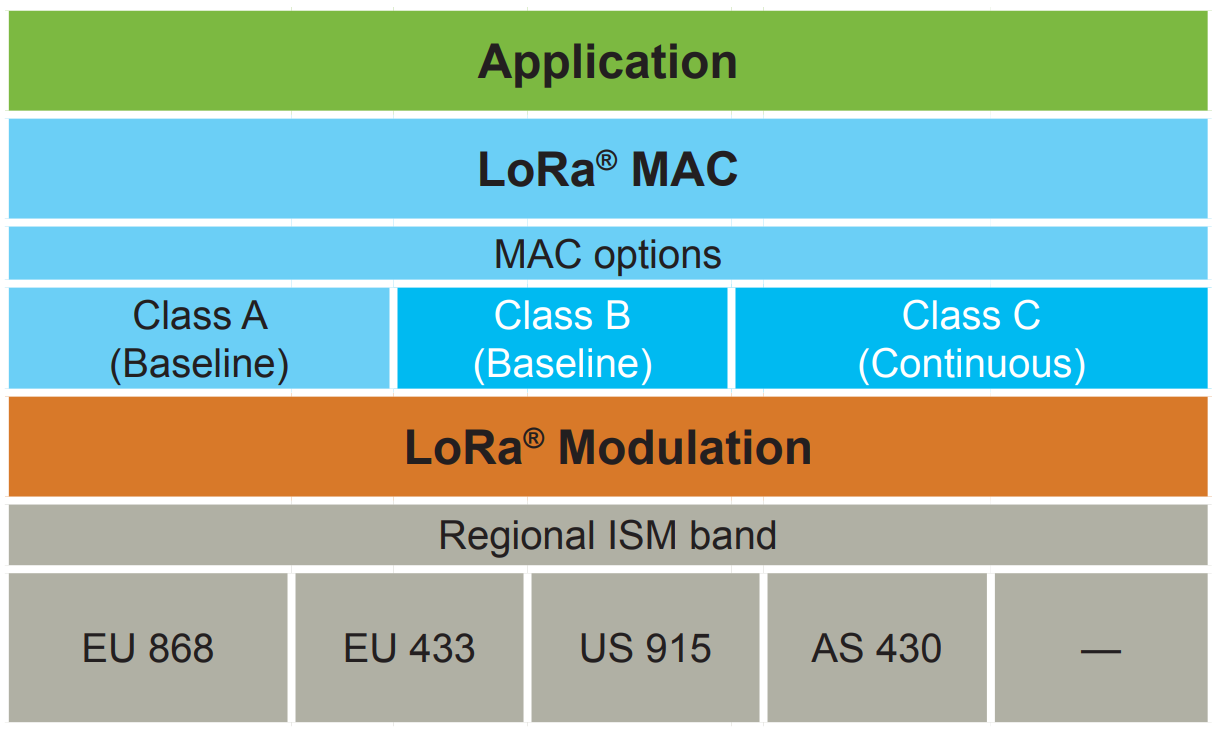
\includegraphics[width=0.65\textwidth]{Figures/Protocols/LoRaWAN/lorawan_and_lora_stack.PNG}
    \caption{Architecture du protocole LoRaWAN}
    \label{fig-lorawan_and_lora_stack}
\end{figure}

L'architecture complète du protocole LoRaWAN est visible en \cref{fig-lorawan_and_lora_stack} à sa base se trouve la couche LoRa comportant différentes fréquences en fonction de la région. Vient ensuite le concept de classe pour les périphériques. Ces classes définissent le comportement des périphériques vis-à-vis du réseau et seront développées plus en détail en \cref{sec-protocols_lorawan_classes}. Vient ensuite toute la partie LoRa MAC avec l'implémentation du protocole LoRaWAN. Toute la formation du paquet avec ses entêtes et ses données se trouve dans ce dernier élément.



\subsection{Classes des périphériques}
\label{sec-protocols_lorawan_classes}

LoRaWAN est un protocole bidirectionnel, assorti de quelques conditions. Il existe trois classes de périphériques. LoRaWAN définit ces trois classes \cite{LoRaWANd15:online} comme ceci : 
\begin{enumerate}
    \item Classe A (\textit{baseline}) : lorsqu'un périphérique envoi un message \textit{uplink}, il se met en écoute durant un laps de temps défini sur deux fenêtres de réception. La séquence de réception pour cette classe est visible sur la \cref{fig-class_a_rx}. C'est la classe qui consomme le moins d'énergie, car l'écoute ne se produit qu'après l'envoi d'un paquet. Quand le périphérique n'est pas ni en émission, ni en écoute de réponse, il peut être placé en veille profonde pour économiser un maximum d'énergie.
    %Dans l'option 1, la \textit{gateway} n'envoi pas de \textit{downlink} après l'\textit{uplink}. A l'inverse dans l'option 2 ou 3, une donnée est envoyée et reçue sur le périphérique. 
    
\begin{figure}[ht!]
    \centering
    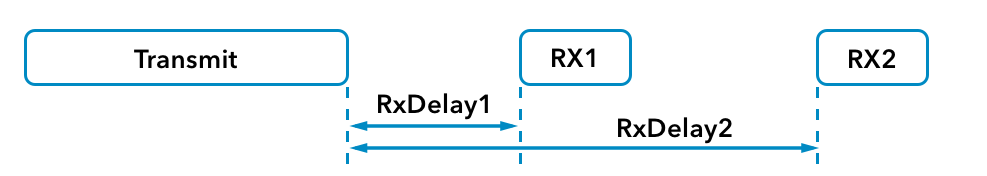
\includegraphics[width=0.9\textwidth]{Figures/Protocols/LoRaWAN/class_a_rx.png}
    \caption{Réception en tant que périphérique de type classe A}
    \label{fig-class_a_rx}
\end{figure}

    
    \item Classe B (\textit{beacon}) : Cette classe est identique à la classe A, mais offre la possibilité supplémentaire de programmer des fenêtres d'écoutes régulières que le périphérique doit écouter. La synchronisation temporelle de ces fenêtres s'effectue à l'aide de \textit{beacons} envoyés par la \textit{gateway} \cite{HomeTheT94:online,}. L'implémentation de cette classe a été finalisée dans la spécification 1.1 de LoRaWAN (cf. \cref{sec-protocols_lorawan_spec_1_1}). La \cref{fig-class_b_rx} illustre cette fenêtre de synchronisation.
   
\begin{figure}[ht!]
    \centering
    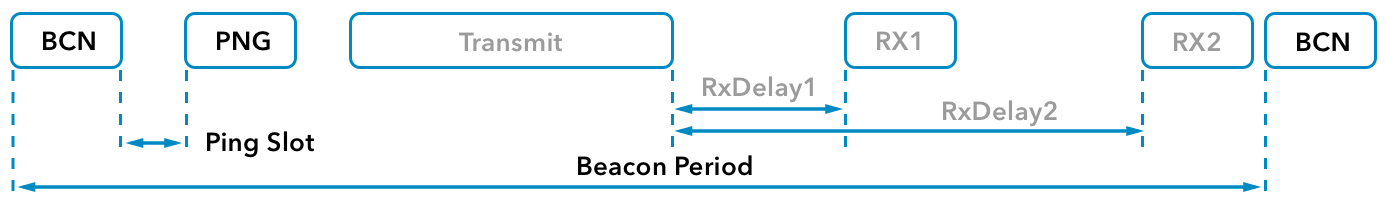
\includegraphics[width=0.9\textwidth]{Figures/Protocols/LoRaWAN/class_b_rx.png}
    \caption{Réception en tant que périphérique de type classe B}
    \label{fig-class_b_rx}
\end{figure} 

    
    \item Classe C (\textit{continuous}) : Cette classe est en écoute permanente sur une des fenêtres de réception, excepté lorsqu'un message est envoyé. On peut voir l'effet sur la \cref{fig-class_c_rx}. Cela a pour avantage de réduire la latence des communications \textit{downlink}, le périphérique n'ayant plus besoin d'un \textit{uplink} pour recevoir le message. En contrepartie, le périphérique consomme en permanence de l'énergie pour recevoir ces données. Cette option est uniquement envisageable si l'autonomie du périphérique ne constitue pas un problème.
    
\begin{figure}[ht!]
    \centering
    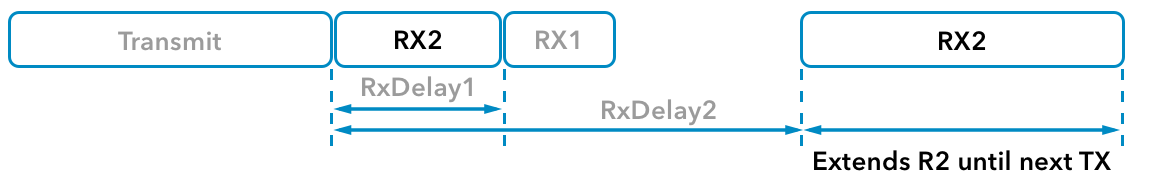
\includegraphics[width=0.9\textwidth]{Figures/Protocols/LoRaWAN/class_c_rx.png}
    \caption{Réception en tant que périphérique de type classe C}
    \label{fig-class_c_rx}
\end{figure}
\end{enumerate}



\subsection{Architecture d'un réseau LoRaWAN}
\label{sec-protocols_lorawan_architecture}
%https://www.tuv.com/media/corporate/products_1/electronic_components_and_lasers/TUeV_Rheinland_Overview_LoRa_and_LoRaWANtmp.pdf


\begin{figure}[ht!]
    \centering
    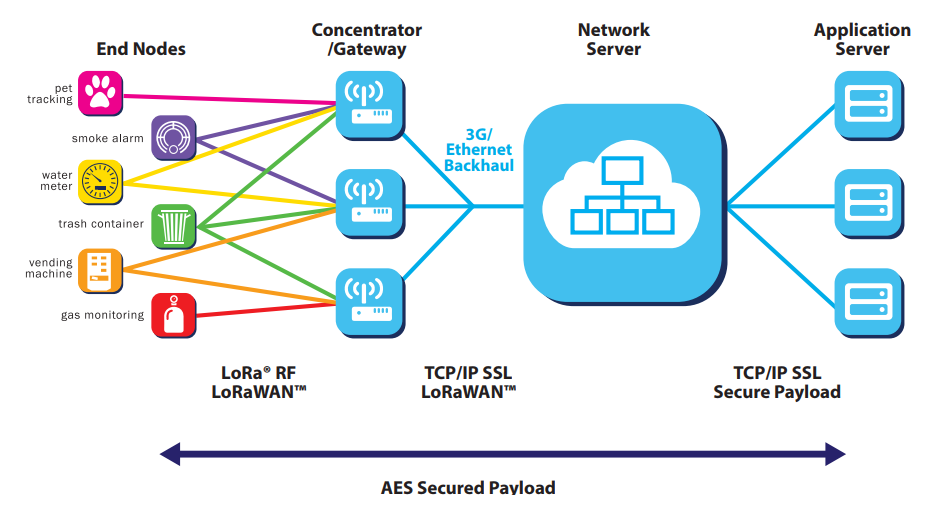
\includegraphics[width=0.95\textwidth]{Figures/Protocols/LoRaWAN/lorawan_archtecture.png}
    \caption{Architecture d'un réseau LoRaWAN}
    \label{fig-lorawan_archtecture}
\end{figure}

La \cref{fig-lorawan_archtecture} illustre l'architecture d'un réseau LoRaWAN avec ses divers composants. Les différents éléments de ce diagramme seront examinés plus en détail dans les sous-sections suivantes.


\subsubsection{\textit{End nodes}}
Les \textit{end nodes} sont les périphériques qui sont connectés au réseau. Ceux-ci sont tous équipés d'un module LoRa de la catégorie \textit{transceivers.}\footnote{\url{https://www.semtech.com/products/wireless-rf/lora-transceivers}}. La carte développée dans le cadre de ce projet entre dans cette catégorie. Un \textit{end node} LoRaWAN est souvent pourvu d'un dispositif basse consommation qui effectue une acquisition et envoie périodiquement des données à une application à travers le réseau. 



\subsubsection{\textit{Gateways}}

Les concentrateurs sont le pont entre un réseau LoRa et un réseau TCP/IP. Ceux-ci sont tous équipés d'un ou plusieurs modules LoRa de type concentrateur\footnote{\url{https://www.semtech.com/products/wireless-rf/lora-gateways}}. Les \textit{gateways} peuvent être achetées directement chez certains fabricants, mais il est également possible de créer sa propre \textit{gateway} à l'aide d'un Raspberry Pi et d'un concentrateur LoRa connecté via une communication série\footnote{\url{https://github.com/ttn-zh/ic880a-gateway/wiki}}. L'une des \textit{gateway} les plus utilisées est la Multitech Conduit, visible sur la \cref{fig-multitech_conduit}.

Le rôle de la \textit{gateway} consiste à démoduler les signaux reçus dans un \textit{buffer} afin de repérer la présence de trames LoRa. Tous les paquets sont transférés au \textit{Network Server}, quand bien même ils ne sont pas du réseau LoRaWAN auquel appartient la \textit{gateway}. Des métadonnées sont également ajoutées au paquet, tel que le \textit{Receive Signal Strength Indicator} (RSSI), \textit{Signal To Noise Ratio} (SNR), le canal de fréquence utilisé, le \textit{data rate}, ainsi que le \textit{Time of Arrival} (ToA). Les \textit{gateways} n'ont aucune information concernant les périphériques connectés au réseau. Elles ne font que transférer les paquets au \textit{Network Server}.

\begin{figure}[ht!]
    \centering
    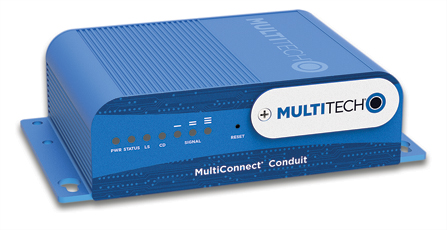
\includegraphics[width=0.4\textwidth]{Figures/Protocols/LoRaWAN/multitech_conduit.jpg}
    \caption{Concentrateur LoRaWAN Multitech Conduit}
    \label{fig-multitech_conduit}
\end{figure}

Les fournisseurs de réseaux doivent offrir un \textit{firmware} compatible avec les \textit{gateways}. Les \textit{firmwares} sont tous basés sur un code fournit par Semtech, nommé \texttt{Lora network packet forwarder}\footnote{\url{https://github.com/Lora-net/packet_forwarder}}. Comme son nom l'indique, ce code a pour but de transférer les données LoRa reçues vers un serveur avec un protocole d'échange spécifique. Le serveur répond ensuite à la \textit{gateway} en fonction de l'action qui doit être effectuée sur le périphérique, par exemple, lorsqu'un objet est autorisé à rejoindre le réseau après une procédure de \texttt{Join}.

\subsubsection{\textit{Network Server}}

Le \textit{Network} \textit{Serveur} est le gestionnaire du réseau. Il s'occupe de tous les paquets reçus sur le port 0. Les données reçues sur les autres ports sont transférées à la couche applicative gérée par l'\textit{Application Server}. Les différentes tâches incombant au \textit{Network Server} sont les suivantes \cite{ttnvideos_network:online} : 
\begin{itemize}
    \item Identification du périphérique qui souhaite communiquer avec le réseau. Les \textit{gateways} redirigent tous les paquets, ceux-ci doivent ensuite être triés \cite{ttnvideos_network:online};
    \item Contrôler le \textit{data rate} si le mode ADR (Adaptative Data Rate) est actif sur le périphérique;
    
    \item Configurer les paramètres radio ainsi que les différents timings des fenêtres de réceptions \cite{ttnvideos_network:online};
    
    \item Gestion des commandes de type MAC\footnote{\url{http://www.rfwireless-world.com/Tutorials/LoRaWAN-MAC-layer-inside.html}} \cite{HomeTheT94:online};
    
    \item Prévenir les attaques de type \textit{replay} en analysant les \textit{frame counters} des paquets;
    
    \item Gestion d'une queue de messages \textit{downlink} qui seront envoyés aux périphériques lors de la réception du prochain message \textit{uplink};
    
    \item Lors de l'envoi d'un message \textit{downlink}, le \textit{Network Server} s'occupe de la sélection de la \textit{gateway} qui doit envoyer le message. Celle-ci est sélectionnée en fonction du RSSI et du SNR vis-à-vis du périphérique sur le message \textit{uplink} reçu \cite{ttnvideos_network:online};
    
    \item Il s'occupe de la gestion du \textit{duty cycle} des \textit{gateways} afin de respecter les normes ETSI \cite{ttnvideos_network:online};
    
    \item Évite les conflits lors de l'envoi de messages \textit{downlink} sur une \textit{gateway}. Une \textit{gateway} ne peut envoyer qu'un seul message à la fois \cite{ttnvideos_network:online}.
\end{itemize}


Cette partie de l'architecture est traitée plus en détail en \cref{sec-stateoftheart_smartcanton}, via la présentation du projet SmartCanton.

\subsubsection{Join Server}

Le \textit{Join Server} n'est pas illustré sur la \cref{fig-lorawan_archtecture}, bien qu'il soit une brique indispensable lors de l'utilisation du mode OTAA. Lors de la réception d'un message de type \textit{Join Request}, le \textit{Network Server} le transfère au \textit{Join Server}. 

Il existe deux modes en LoRaWAN pour rejoindre un réseau. Le premier mode se nomme \textit{Over-the-Air Activation} (OTAA). Dans le mode OTAA, seules l'\texttt{App Key} et l'adresse \texttt{Dev EUI} (comparable à l'adresse MAC d'un périphérique) doivent être connues sur le périphérique. Le \texttt{Join Server} vérifie si le périphérique a été préalablement enregistré dans une base de données contenant une \texttt{App Key}, un \texttt{App EUI} (optionnel selon les cas), ainsi qu'un \texttt{Dev EUI}. Si tel est le cas, un \texttt{Join Accept} est retourné au périphérique qu'il a été accepté sur le réseau. Avec ce \textit{Join Accept}, il reçoit son \texttt{Dev Address} qui lui permet d'émettre sur le réseau avec cette adresse, ainsi les éléments nécessaires à la \texttt{Network Session Key} et \texttt{App Session Key} pour la communication. La procédure du \texttt{join} du mode OTAA est observée en détail en \cref{sec-security_lorawan} de ce document.

L'autre mode est \textit{Activation by Personalization} (ABP). Dans ce mode, toutes les informations nécessaires doivent être prodiguées manuellement au périphérique. Il faut donc spécifier le \textit{Device EUI} (normalement fixé par le fabricant), l'\textit{Application EUI}, le \textit{Device Address}, la \textit{Network Session Key}, ainsi que l’\textit{App Session Key}.

Le mode OTAA est préféré au mode ABP, non seulement parce qu'il simplifie l'ajout d'un périphérique au réseau, mais également parce qu'il ajoute un aspect de sécurité (cf. \cref{sec-security_lorawan}).

\subsubsection{Applications Server}


Le serveur d'application reçoit tous les paquets qui n'ont pas été envoyés sur le port 0. Toutes les \textit{payload} sont déchiffrées par ce serveur. Les données sont ensuite mises à disposition de l'utilisateur. Certains fournisseurs de réseau proposent des interfaces Web complètes pour visualiser les données décodées avec la \textit{App Session Key}. Ils offrent également la possibilité de rediriger ces données vers des fournisseurs d'application, par exemple Cayenne de MyDevices, qui accélèrent les prototypages rapides d'applications. Certains fournisseurs sont plus minimalistes et n'offrent qu'une interface de récolte de données à l'aide d'API diverses et variées. 

L'application finale est quant à elle entièrement libre pour l'utilisateur, la seule contrainte étant l'interface de communication proposée par le fournisseur de réseau. Chaque fournisseur peut proposer l'interface qu'il désire. Par exemple, TTN propose une interface basée sur un flux MQTT\footnote{\url{http://mqtt.org/}} et développe actuellement une interface AMQP\footnote{\url{https://www.amqp.org/}}. 


\subsection{\textit{Spreading Factor} et \textit{Data Rate}}
\label{sec-protocols_lorawan_spreading_factor}
%https://docs.exploratory.engineering/lora/dr_sf/


\begin{figure}[ht!]
    \centering
    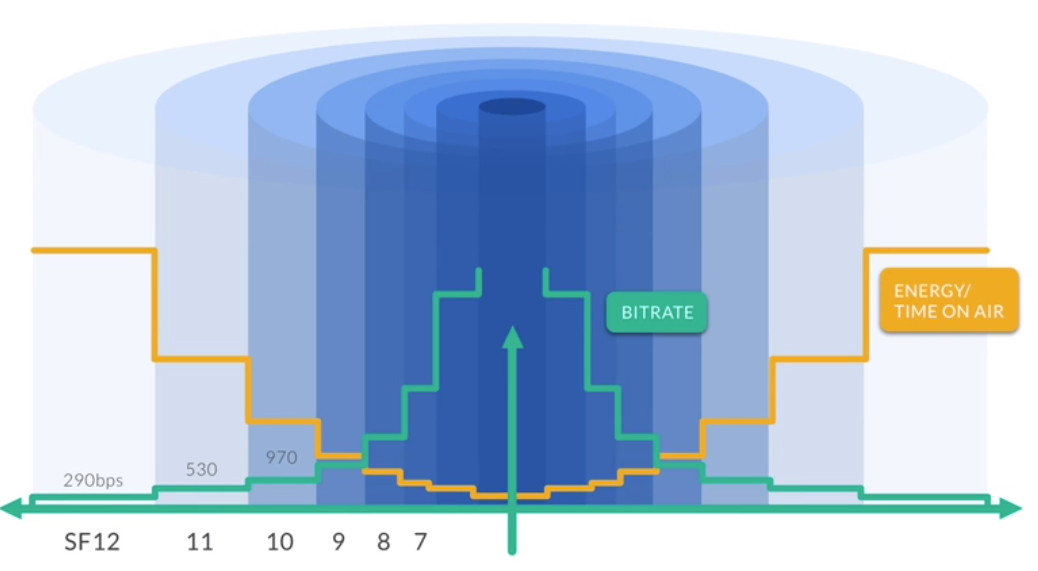
\includegraphics[width=0.7\textwidth]{Figures/Protocols/LoRaWAN/lora_datarate_airtime.png}
    \caption{Comparatif du temps d'émission d'une trame LoRaWAN en fonction de ses paramètres}
    \label{fig-lora_datarate_airtime}
\end{figure}

Le \textit{Spreading Factor} a d'ores et déjà été introduit en \cref{sec-stateoftheart_lora_spread_factor} lors de la présentation de la modulation LoRa. LoRaWAN utilise non seulement les SF pour l'émission, mais il ajoute également le concept de \textit{Data Rate} (DR). Le \cref{tab-datarate_eu} présente tous les \textit{data rate} qui sont autorisés en Europe \cite{Explorat95:online}. Chaque région possède des \textit{data rate} différents en fonction des législations. Chaque DR a une configuration différente en se basant sur un SF et sur la bande passante assignée. On constate en observant le \cref{tab-datarate_eu} que plus le DR est faible, plus le débit est faible. Avec un SF plus élevé, le temps d'émission est supérieur, ce qui a pour conséquence d'augmenter la portée en accentuant la sensibilité du récepteur. La taille du \textit{payload} est également affectée par le temps d'émission,et ce, afin d'éviter qu'on ne sature trop le réseau lors de l'émission avec un SF élevé. Une illustration plus visuelle de l'effet du DR est visible sur la \cref{fig-lora_datarate_airtime}.


\begin{table}[ht!]
\centering
\caption{Différents \textit{data rate} LoRaWAN avec leurs débits pour l'Europe}
\label{tab-datarate_eu}
\begin{tabular}{|l|l|r|r|}
\hline
\rowcolor[HTML]{BBDAFF} 
\multicolumn{1}{|c|}{\cellcolor[HTML]{BBDAFF}\textit{\textbf{Data Rate}}} & \multicolumn{1}{c|}{\cellcolor[HTML]{BBDAFF}\textbf{Configuration}} & \multicolumn{1}{c|}{\cellcolor[HTML]{BBDAFF}\textit{\textbf{bits/s}}} & \multicolumn{1}{c|}{\cellcolor[HTML]{BBDAFF}\textit{\textbf{Max payload}}} \\ \hline
DR0 & SF12/125kHz & 250 & 59 \\ \hline
DR1 & SF11/125kHz & 440 & 59 \\ \hline
DR2 & SF10/125kHz & 980 & 59 \\ \hline
DR3 & SF9/125kHz & 1 760 & 123 \\ \hline
DR4 & SF8/125kHz & 3 125 & 230 \\ \hline
DR5 & SF7/125kHz & 5 470 & 230 \\ \hline
DR6 & SF7/250kHz & 11 000 & 230 \\ \hline
DR7 & FSK: 50kbps & 50 000 & 230 \\ \hline
\end{tabular}
\end{table}


Pour éviter de fixer une valeur qui ne sera pas efficace dans toutes les situations, il est possible d'utiliser l'\textit{Adaptive Data Rate} (ADR) \cite{HomeTheT94:online}. L'ADR est un mécanisme qui a pour but d'optimiser les débits de données, le temps d'émission et, par conséquent, la consommation énergétique. L'ADR ne doit être utilisé que par des n\oe uds statiques. Ce sont les n\oe uds qui décident si cette option est activée ou non. Lorsque le réseau est informé de l'utilisation de l'ADR, celui-ci sauvegarde les 20 transmissions les plus récentes avec le \textit{frame counter}, \textit{signal-to-noise ratio} (SNR) et le nombre de \textit{gateways} qui ont reçu le paquet.

L'algorithme utilisé est décrit dans une \textit{application note} de Semtech, nommée \textit{Simple rate adaptation recommended algorithm}\footnote{\url{https://github.com/TheThingsNetwork/ttn/issues/265\#issuecomment-255092765}}.


\subsection{Paquets LoRaWAN}

\begin{figure}[ht!]
    \centering
    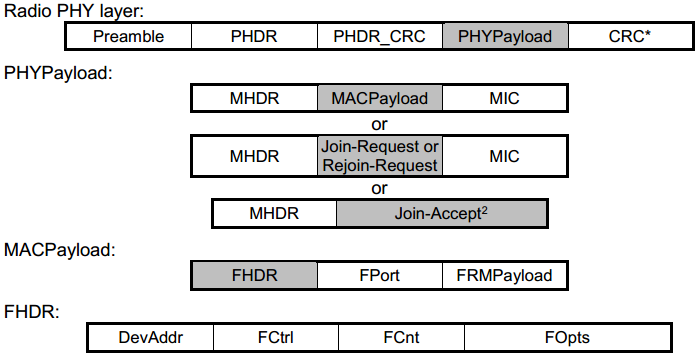
\includegraphics[width=0.9\textwidth]{Figures/Protocols/LoRaWAN/lorawan_mac_format_packets.png}
    \caption{Format des messages du protocole LoRaWAN}
    \label{fig-lorawan_mac_format_packets}
\end{figure}


Les paquets LoRaWAN se basent sur les paquets LoRa pour la transmission. Le squelette d'un paquet LoRa a d'ores et déjà été présenté en \cref{sec_stateOfTheArtLoRa}. Tous les paquets de données disposent d'une \texttt{PHY \textit{payload}} commençant par un octet de \textit{MAC header} (\texttt{MHDR}), suivi d'un \texttt{MAC \textit{payload}} (\texttt{MACPayload}). Le champ \texttt{PHYPayload} contient toute l'implémentation du protocole LoRaWAN. L'encapsulation des paquets au fil des différentes couches est visible sur la \cref{fig-lorawan_mac_format_packets}.


\begin{table}[ht!]
\centering
\caption{Différents champs contenus dans un MHDR}
\label{tab-header_MHDR_content}
\begin{tabular}{
>{\columncolor[HTML]{BBDAFF}}l |l|l|l|}
\cline{2-4}
\textbf{\textit{Bit\#}} & 7..5 & 4..2 & 1..0 \\ \hline
\textbf{\textit{MHDR bits}} & MType & RFU & Major \\ \cline{2-4} 
\end{tabular}
\end{table}

\begin{table}[ht!]
\centering
\caption{Différents types de messages MAC possibles}
\label{tab-mac_message_types}
\begin{tabular}{|l|l|}
\hline
\rowcolor[HTML]{BBDAFF} 
\multicolumn{1}{|c|}{\cellcolor[HTML]{BBDAFF}\textbf{\textit{MType}}} & \multicolumn{1}{c|}{\cellcolor[HTML]{BBDAFF}\textbf{\textit{Description}}} \\ \hline
000 & Join-request \\ \hline
001 & Join-accept \\ \hline
010 & Unconfirmed Data Up \\ \hline
011 & Unconfirmed Data Down \\ \hline
100 & Confirmed Data Up \\ \hline
101 & Confirmed Data Down \\ \hline
110 & Rejoin-request \\ \hline
111 & Proprietary \\ \hline
\end{tabular}
\end{table}

Les payload peuvent contenir différents types de paquets, ceux-ci étant définis dans l'entête MHDR dont les champs sont visibles sur la \cref{tab-header_MHDR_content}. Le type de message est codé sur 3 bits dans un champ nommé \texttt{MType}. LoRaWAN implémente 8 types de paquets visibles sur le \cref{tab-mac_message_types}. Les messages envoyés par les périphériques sont de types \texttt{Data UP}. Ceux-ci peuvent être confirmés ou non selon le type d'utilisation désirée. Le champ RFU signifie \textit{Reserved for Future Use} et le champ Major est utilisé pour spécifier la version de la spécification LoRaWAN utilisée (1.0 ou 1.1 actuellement).

La description complète des paquets est disponible dans le chapitre \texttt{MAC Message Formats} du document \texttt{LoRaWAN 1.1 Specification}\footnote{\url{https://www.lora-alliance.org/lorawan-for-developers}} de la LoRa Alliance. 


\subsection{Clés de chiffrement}

\begin{figure}[ht!]
    \centering
    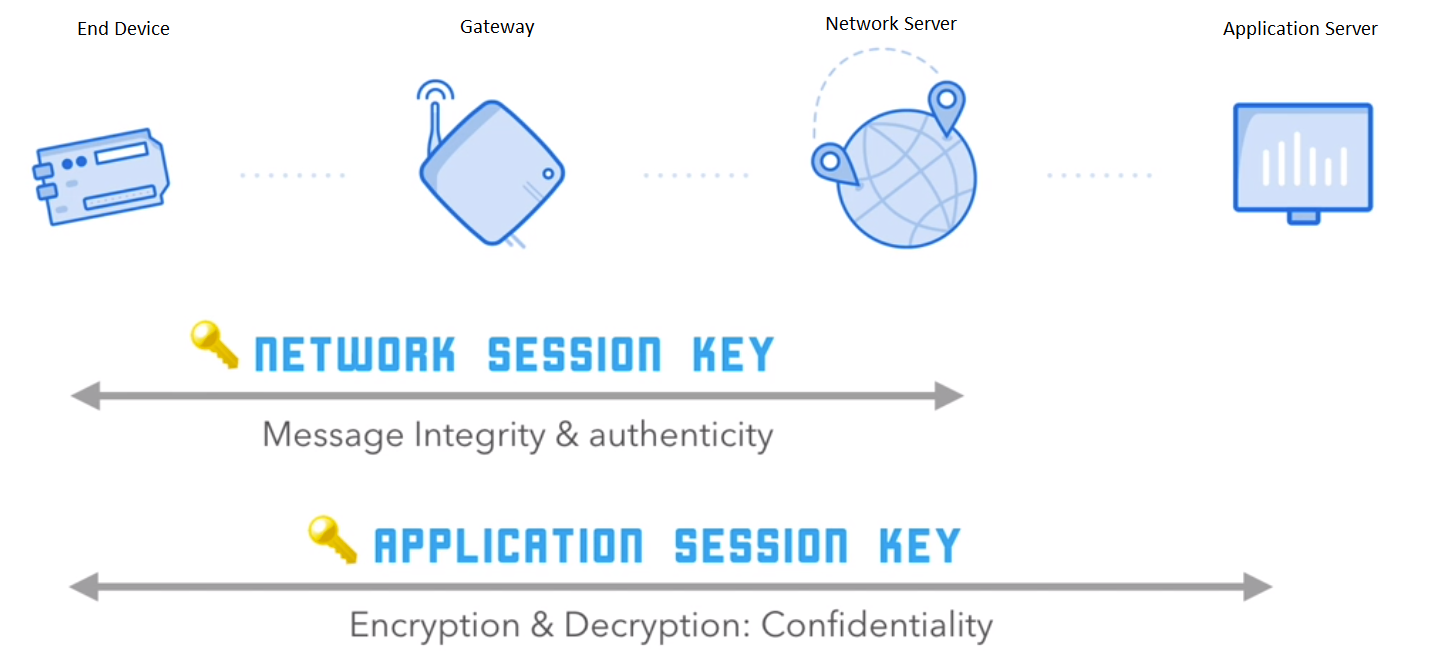
\includegraphics[width=0.8\textwidth]{Figures/Protocols/LoRaWAN/keys_explained.PNG}
    \caption{Rôles de la \textit{Network Session Key} et \textit{Application Session Key}}
    \label{fig-keys_explained}
\end{figure}

En OTAA, lorsqu'un périphérique souhaite rejoindre un réseau il ne dispose que d'une seule et unique clé, nommée AppKey. Une fois le réseau LoRaWAN rejoint, deux autres clés sont créées. L'aspect sécurité de ces clés, ainsi que la génération de celles-ci est vue plus en détail en \cref{sec-security_lorawan} de ce document. Pour l'heure, voici une liste des trois clés indispensables et leurs rôles respectifs : 
\begin{enumerate}
    \item \texttt{App Key} : doit être connue par le \textit{Join Server} et par le périphérique. C'est un secret partagé qui doit être bien gardé, puisque toutes les clés sont générées grâce à lui.
    \item \texttt{Network Session Key} : clé utilisée pour chiffrer les communications entre le périphérique et le \textit{Network Server}. Cette clé est générée à l'aide de l'App Key.
    \item \texttt{Application Session Key} : clé utilisée pour chiffrer les communications entre le périhpréqiue et l'\textit{Application Server}. Elle est également générée à l'aide de l'App Key.
\end{enumerate}

Sur la \cref{fig-keys_explained}, on peut visualiser l'utilisation des clés en fonction des types de messages envoyés.


% \subsection{Rejoindre un réseau LoRaWAN}


% Il existe deux modes en LoRaWAN pour rejoindre un réseau. Le premier est le mode \textit{Over-the-Air Activation} (OTAA). Dans le mode OTAA, la seule qui doit être connue sur le périphérique est la \texttt{App Key} ainsi que l'adresse \texttt{Dev EUI}. Le \texttt{Join Server} vérifie si le périphérique a été préalablement enregistré dans une base de données contenant une \texttt{App Key}, une \textit{App EUI} (optionnelle selon les cas) ainsi qu'une \texttt{Dev EUI}. Si c'est bien le cas, un \texttt{Join Accept} est retourné au périphérique lui indiquant qu'il a été accepté sur le réseau. Avec ce \textit{Join Accept}, il reçoit son \texttt{Dev Address} afin de pouvoir émettre sur le réseau au moyen de cette adresse. Il reçoit également les élément pour générer sa \texttt{Network Session Key} et \texttt{App Session Key} pour communication. La procédure du \texttt{join} du mode OTAA est détaillée en profondeur en \cref{sec-security_lorawan} de ce document.

% Le second mode se nomme \textit{Activation by Personalization} (ABP). Dans ce mode, toutes les informations nécessaires doivent être prodiguées manuellement au périphérique. Il faut donc spécifier le \textit{Device EUI} (normalement fixé par le fabricant), l'\textit{Application EUI}, la \textit{Device Address}, la \textit{Network Session Key}, ainsi que la \textit{App Session Key}.

% Le mode OTAA est préféré au mode ABP, non seulement parce qu'il simplifie l'ajout d'un périphérique au réseau, mais également parce qu'il ajoute un aspect de sécurité (cf. \cref{sec-security_lorawan}).





\subsection{Canaux d'émission}

La spécification LoRaWAN définit 3 canaux communs de 125 kHz pour la bande des 868 MHz (868.10, 868.30 et 868.50 MHz)\cite{HomeTheT94:online}. Ces canaux doivent être obligatoirement supportés par tous les réseaux LoRaWAN et par tous les périphériques. Ces 3 canaux sont ceux utilisés par tous les périphériques pour rejoindre un canal. Pendant la procédure de \texttt{Join}, le réseau peut demander aux périphériques d'ajouter de nouveaux canaux à sa liste. Ces canaux sont utilisés en \texttt{downlink}, mais également en \texttt{uplink}\cite{HomeTheT94:online}.



\subsection{Temps d'émission et nombre de paquets}

Le \textit{duty cycle} d'émission a été abordé en \cref{sec-stateoftheart_lora_dutycycle}. Les pourcentages d'utilisation des bandes de fréquences limitent les utilisations qui peuvent être faites de ce protocole. Le temps d'émission est affecté par les paramètres choisis pour l'émission. Comme expliqué en \cref{sec-stateoftheart_lora_spread_factor} et en \cref{sec-protocols_lorawan_spreading_factor}, le \textit{spreading factor} et le \textit{coding rate} augmentent considérablement le temps d'émission. 


Outre ces restrictions, certains fournisseurs de réseau limitent encore plus drastiquement l'utilisation de la bande de fréquence. Par exemple, \textit{The Things Network} (TTN) applique une \textit{Fair Access Policy} \footnote{\url{https://www.thethingsnetwork.org/forum/t/limitations-data-rate-packet-size-30-seconds-uplink-and-10-messages-downlink-per-day-fair-access-policy/1300}} afin de réduire la charge d'accès sur leur réseau \cite{Limitati95:online}. Les types de limitations sont les suivantes : 
\begin{enumerate}
    \item Une moyenne de 30 secondes en émission \textit{uplink}, par jour et par périphérique;
    \item Maximum 10 \textit{downlink} messages par jour, en incluant des confirmations pour les messages de type \textit{confirmed uplink};
    \item Les périphériques avec un SF de 11 ou 12 \textbf{fixe} ne sont pas autorisés à rejoindre le réseau (ceci ne s'applique pas aux périphériques avec l'ADR activé).
\end{enumerate}

La limitation de 30 secondes d'émission est la plus restrictive. Par exemple, si un périphérique envoi un \textit{payload} de 55 bytes en utilisant le \textit{data rate} le plus élevé, cela crée une émission de 71.81 millisecondes\cite{Limitati95:online}. En respectant uniquement les standards européens, ceci signifie qu'un périphérique doit attendre 71,09 secondes avant de pouvoir envoyer une nouvelle trame. Cependant, avec la limitation supplémentaire de TTN, le périphérique ne peut envoyer que 417 paquets de 71.81 par jours; ce qui signifie en moyenne un paquet toutes les 207 secondes ainsi en appliquant ces limitations, une \textit{gateway} TTN peut avoir jusqu'à 1000 n\oe uds connectés \cite{Limitati95:online}. TTN propose un tableau sur Google Sheet\footnote{\url{https://docs.google.com/spreadsheets/d/1QvcKsGeTTPpr9icj4XkKXq4r2zTc2j0gsHLrnplzM3I}} éditable pour calculer le nombre de paquets possibles sur le réseau en fonction de la configuration appliquée sur le périphérique.

\subsection{Spécification LoRaWAN 1.1}
\label{sec-protocols_lorawan_spec_1_1}

La LoRa Alliance a finalisé la spécification V1.1 en octobre 2017\footnote{\url{https://www.lora-alliance.org/lorawan-for-developers}}. Il faut à présent du temps pour qu'elle se démocratise sur les différents périphériques. Actuellement, le CMWX1ZZABZ ne propose pas de \textit{firmware} pour le support de cette spécification. Celle-ci ne nécessite par ailleurs pas de nouveau matériel, son implémentation étant entièrement logicielle. Certaines nouveautés sur la sécurité sont exposées en \cref{sec-security_lorawan_1_1}. 

\begin{figure}[ht!]
    \centering
    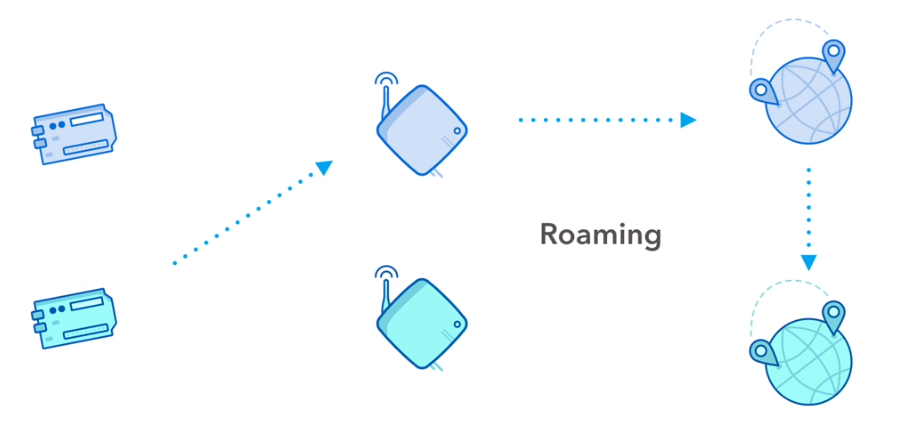
\includegraphics[width=0.6\textwidth]{Figures/Protocols/LoRaWAN/lorawan_roaming.png}
    \caption{Roaming LoRaWAN}
    \label{fig-lorawan_roaming}
\end{figure}

LoRaWAN 1.1 ajoute le support du \textit{roaming} entre différents opérateurs. Le concept est visible sur la \cref{fig-lorawan_roaming}, où l'on peut voir un périphérique transmettant un paquet capturé par une \textit{gateway} d'un réseau auquel il n'appartient pas. Si le \textit{Network Server} ne reconnait pas le périphérique comme appartenant à son réseau, il \textit{forward} les paquets vers le \textit{Network Server} de l'opérateur d'origine. Le principe général est identique au \textit{roaming} appliqué à la téléphonie mobile.




\chapter{Sécurité}






\section{IEEE 802.15.4 et les protocoles dérivés}

Étant donné que le microcontrôleur choisi supporte le standard IEEE 802.15.4, il est intéressant de faire une petit analyse sur la sécurité implémentée dans ce standard. 

Le standard IEEE 802.15.4 décrit des procédures de sécurité. Le standard décrit quel algorithme de cryptage doit être utilisé pour chiffrer les données à transmettre \cite{Security81:online}. Cependant, le standard ne spécifie pas comment les clés doivent être échangées ni l'authentification de celles-ci. Le standard laisse cela aux couches supérieures. 


Le protocole ZigBee, qui est le protocole le plus répendu basé sur le standard IEEE 802.15.2.


% IEEE 802.15.4 sets the encryption algorithm to use when cyphering the data to transmit, however,  the standard does not specify how the keys have to be managed or what kind of authentication policies have to be applied. These issues are treated in the upper layers which are managed by technologies such as ZigBee.


\section{Bluetooth}




\section{LoRa}
\label{sec_lora_security}





\chapter{Conception matérielle}
\label{3_hardware}

Ce chapitre présente toute l'implémentation de la carte électronique qui a été réalisée dans le cadre de ce projet. La description des composants, de même que le choix de ceux-ci y sont évoqués.


\section{Introduction}

Le présent projet avait pour objectif premier la réalisation d'une carte électronique. Les différents composants à placer sur cette carte ont été choisis en fonction des besoins de certains \textit{use cases} exposés à la DGSI. Voici une liste contenant quelques exemples : 
\begin{itemize}
    \item Un traqueur GPS transmettant la position par LoRa;
    \item Un détecteur de vol avec détection de mouvement transmettant ensuite la position par LoRa une fois l'objet en mouvement;
    \item Un scanneur Bluetooth permettant de détecter un certain nombre de \textit{beacons} autour d'une borne;
    \item Une station météorologique avec la possibilité de mesurer la qualité de l'air ambiant.
\end{itemize}

Ces exemples ont ainsi permis la mise en place d'une liste de périphériques indispensables à la carte.\\

Un nouveau concept de partage de clé a également été imaginé, avec la possibilité de changer l’App Key LoRaWAN présente sur le périphérique via l'utilisation d'un simple smartphone. Il fallait dès lors choisir une méthode d'accès au périphérique. La quantité de données transférées étant faible (de l'ordre de quelques centaines de bytes par secondes, au grand maximum) et le dispositif devant être utilisable sur batterie, le Bluetooth Low Energy a été retenu. Le Bluetooth est une technologie qui avait déjà été retenue pour l'implémentation du scanneur de périphériques.\\

Tous les documents liés au circuit électronique (schémas, modèles 3D et footprints) sont disponibles dans l'\cref{AppendixDevBoxHardware}.

\section{Architecture}

Pour une plus grande flexibilité de la carte de développement, il est judicieux d'utiliser deux processeurs sur la carte électronique, ce qui implique deux implémentations possibles. Les \cref{fig-hardware_option1} et \cref{fig-hardware_option2} illustrent ces deux options. La première consiste à utilise un processeur LoRa comme processeur principal du système; soit un processeur sur lequel la communication LoRa est gérée en plus de la gestion des différents périphériques de la carte. Par exemple, un GPS, un accéléromètre, etc. Le processeur gérant le Bluetooth serait ainsi un simple périphérique pour le processeur LoRa. Une API doit être mise en place pour faciliter l'échange d'informations entre les deux. La deuxième possibilité est d'inverser les rôles des processeurs. Le processeur principal serait celui qui gère les protocoles en 2.4 GHz et communique périodiquement avec le processeur LoRa afin d'envoyer et recevoir des données provenant du réseau.

\begin{figure}[ht!]
    \centering
    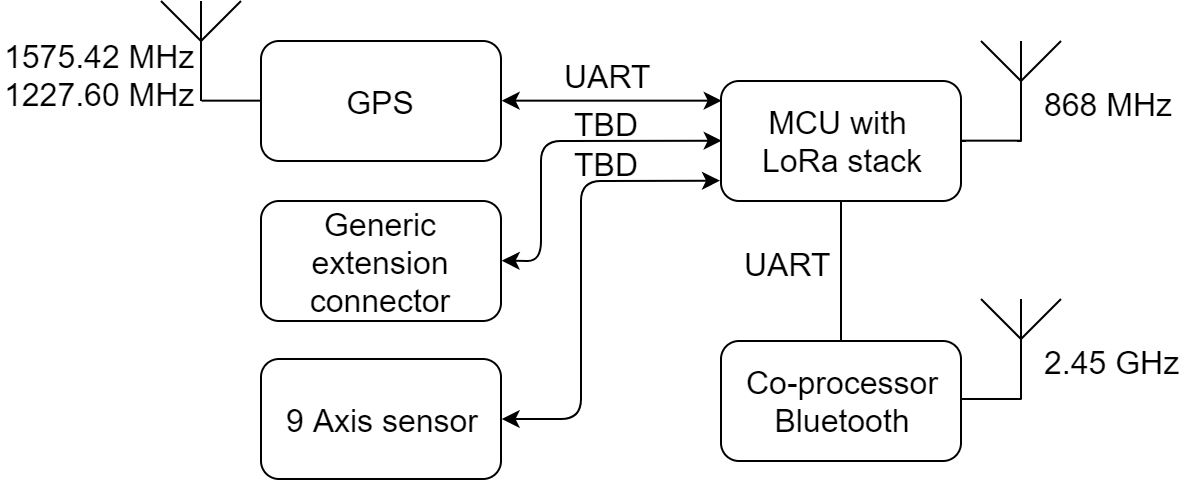
\includegraphics[width=\textwidth]{Figures/Hardware/master_onepage_option1.png}
    \caption{Architecture option numéro 1}
    \label{fig-hardware_option1}
\end{figure}

\begin{figure}[ht!]
    \centering
    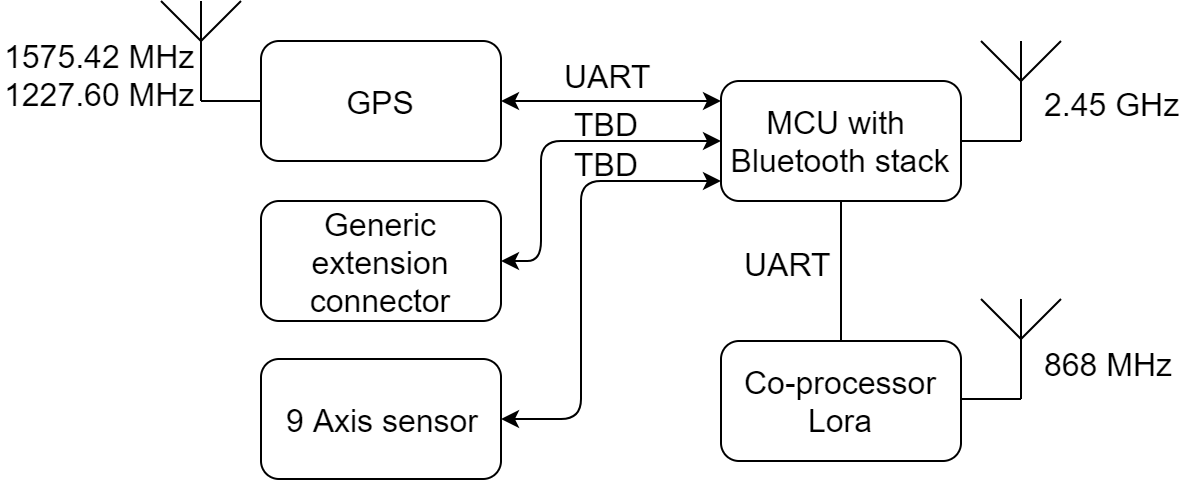
\includegraphics[width=\textwidth]{Figures/Hardware/master_onepage_option2.png}
    \caption{Architecture option numéro 2}
    \label{fig-hardware_option2}
\end{figure}

L'architecture choisie est l'option numéro 2. Nous avons donc tous les périphériques qui sont connectés au processeur s'occupant du Bluetooth. Le processeur avec l'interface LoRa, lui ne s'occupe, quant à lui, que de communiquer les évènements de réception de données et de transférer les messages provenant depuis le processeur Bluetooth. Il est également plus simple de faire une API pour le LoRa, le nombre de données et paramètres configurables étant moins important que dans le cas des communications Bluetooth. Si on souhaite faire une API entre les deux processeurs, il est ainsi nécessaire de tenir compte de la complexité de ceux-ci. Les accès LoRa sont également plus ponctuels. Le nombre de paquets envoyés par heures est très faible, en comparaison avec ce qui est réalisable en Bluetooth. On peut ainsi faire en sorte que le processeur soit en mode très basse consommation en attendant une commande de la part du processeur principal ou la réception d'un paquet LoRa sur son antenne.


\section{Choix des composants et leurs caractéristiques}

Cette section a pour but d'une part d'expliquer les différents choix effectués pour les composants présents sur la DevBox et, d'autre part, de présenter les caractéristiques principales des composants les plus importants.

\subsection{Microcontrôleur}
\label{subsect:microcontroleur}

Le microcontrôleur est le c\oe ur de ce projet; c'est dans celui-ci que la plus grande partie du développement va se produire. Il est dès lors important de sélectionner le composant idéal pour notre application, car une fois la sélection faite et les cartes électroniques réalisées, il est impossible de le changer sans générer des changements conséquents. Pour éviter cela, une étude des divers microcontrôleurs disponibles sur le marché a été réalisée.

\subsubsection{Critères de comparaison}
Le microcontrôleur a dû être choisi judicieusement en fonction du cahier des charges. Un comparatif, visible sur le \cref{tab-mcu_table}, a donc été effectué.  L'un des premiers points retenus est le type de protocoles qui sont supportés par le microcontrôleur. Le Bluetooth Low Energy étant un prérequis, il nous a été possible de procéder à un premier filtre, ce qui explique également que tous les microcontrôleurs affichés disposent de cette fonctionnalité. Néanmoins, le Bluetooth Low Energy s'accompagne de la norme 4.2, annoncée le 2 décembre 2014 \cite{Bluetoot59:online}, et de la norme 5.0, annoncée quant à elle le 16 juin 2016. Cette dernière n'était malheureusement pas encore parfaitement supportée par tous les fabricants de microcontrôleurs. Comme précédemment expliqué en \cref{sec_2_4_GHz}, une simple mise à jour logicielle permet de promouvoir un microcontrôleur en Bluetooth 5.0, du moins, en garantissant les fonctionnalités primordiales du protocole. Les microcontrôleurs affichés dans le tableau disposaient, en date du 1er octobre 2017, uniquement des fonctionnalités listées, ce qui ne signifie toutefois pas qu'elles ne peuvent pas s'agrandir avec le temps. \\

Après le Bluetooth, le deuxième type de protocole est le IEEE 802.15.4 \cite{IEEE802137:online}. Ce standard IEEE n'est pas un protocole en tant que tel, mais un modèle qui est respecté par plusieurs protocoles. Parmi les protocoles qui utilisent ce standard, on retrouve le ZigBee, WirelessHART, MiWi, SNAP, ou encore le Thread. Ce standard est de plus en plus utilisé pour la domotique. En effet, il permet de facilement créer des réseaux maillés permettant ainsi une grande couverture de l'habitation.\\

Enfin, un moyen de communication en dessous d'un gigahertz était également envisageable. Si le processeur supporte cela, ce peut être un avantage pour la réalisation de futurs \textit{use cases}. Néanmoins, la communication dans cette plage de fréquence a quelques désavantages, en commençant par la taille de l'antenne qu'il faut utiliser. La consommation du processeur est également affectée, pouvant atteindre jusqu'à 100 mA (cf. EFR32M datasheet). LoRa entre dans cette catégorie, mais seuls les processeurs fournis par Semtech peuvent implémenter la modulation. Ils ne sont, à l'heure actuelle, pas assez développés pour pouvoir être utilisés comme unique processeur gérant du 2.4 GHz avec en parallèle une interface LoRa (868 ou 433 MHz). \\

On a ensuite l'aspect consommation lors de l'émission qui entre en jeu. Afin d'être le plus proche possible en termes de comparaison entre les différents modèles, la consommation en émission a été retenue pour la fréquence de 2.4 GHz avec une puissance de 0 dBm en sortie. Plus cette consommation est faible, plus notre système aura la possibilité d'être autonome grâce à sa batterie. Finalement, les deux derniers points à retenir sont la taille des mémoires (RAM et Flash), qui selon leur taille nous permettent de faire un programme plus complexe, puis le coût à l'unité du microcontrôleur. Les prix ont été sélectionnés pour une seule unité sur le site d'achat Mouser\footnote{\url{http://www.mouser.ch/}} Suisse. \,

Davantage d'éléments auraient pu être pris en compte pour la comparaison, à l'instar des périphériques disponibles ou la possibilité d'avoir une matrice d'assignation des pins, utile lorsque l'on souhaite avoir des cartes modulables. Ce qui est primordial, c'est d'avoir au minimum une interface de communication série (SPI, I2C ou UART), étant précisé que tous ces microcontrôleurs en ont plusieurs de disponibles. Il convient également de prendre en considération la consommation du microcontrôleur, surtout dans les modes de sommeil. Celle-ci se trouve dans la même plage pour tous les microcontrôleurs listés, soit aux environs des 200\,\si{\micro}A avec une vitesse du microcontrôleur réduite au minimum, tous les périphériques désactivés et la persistance des données en RAM. Pour sortir de ces modes, le réveil émane habituellement d'une interruption matérielle, de sorte à pouvoir continuer à exécuter le code une fois sorti de veille. Vu que la carte de développement finale sera équipée d'un GPS, lequel sera le point principal de la consommation, cette donnée n'a pas été intégrée dans le tableau, bien qu'elle soit observée sur chaque microcontrôleur.\\

\begin{sidewaystable}[!ht]
\centering
\caption{Comparaison des microcontrôleurs envisagés pour le projet}
\begin{tabular}{|l|l|l|c|c|c|c|l|l|c|c|l|}
\hline
\multicolumn{1}{|c|}{\textbf{Manufacturer}} & \multicolumn{1}{c|}{\textbf{Model}} & \multicolumn{1}{c|}{\textbf{CPU}} & \textbf{\begin{tabular}[c]{@{}c@{}}BLE\\ 4.2\end{tabular}} & \textbf{\begin{tabular}[c]{@{}c@{}}BLE\\ 5.0\end{tabular}} & \textbf{\begin{tabular}[c]{@{}c@{}}IEEE\\     802.15.4\end{tabular}} & \textbf{\begin{tabular}[c]{@{}c@{}}Sub\\     1GHz\end{tabular}} & \multicolumn{1}{c|}{\textbf{\begin{tabular}[c]{@{}c@{}}Receive \\     Current\end{tabular}}} & \multicolumn{1}{c|}{\textbf{\begin{tabular}[c]{@{}c@{}}Transmit\\ Current \\ (@ 2.4Ghz, \\ @ 0dBm)\end{tabular}}} & \textbf{\begin{tabular}[c]{@{}c@{}}Flash/\\     SRAM\end{tabular}} & \textbf{\begin{tabular}[c]{@{}c@{}}Disponi-\\     bility\end{tabular}} & \multicolumn{1}{c|}{\textbf{Price}} \\ \hline
NXP & KW41Z & \begin{tabular}[c]{@{}l@{}}Cortex\\ M0+\\@ 48 MHz\end{tabular} & Yes & No & Yes & No & 6.8 mA & 6.1 mA & \begin{tabular}[c]{@{}c@{}}512 kB\\ / 128 kB\end{tabular} & Yes & 6.34 CHF \\ \hline
NXP & QN908x & \begin{tabular}[c]{@{}l@{}}Cortex\\ M4F\\@ 32 MHz\end{tabular} & Yes & Yes & No & No & 3.4 mA & 3.4 mA & \begin{tabular}[c]{@{}c@{}}512 kB\\ / 128 kB\end{tabular} & Yes & 5.87 CHF \\ \hline
\begin{tabular}[c]{@{}l@{}}Texas\\     Instrument\end{tabular} & CC2650 & \begin{tabular}[c]{@{}l@{}}Cortex\\ M3\\@ 48 MHz\\+ M0 for RF\end{tabular} & Yes & No & Yes & No & 6.2 mA & 6.8 mA & \begin{tabular}[c]{@{}c@{}}128 kB\\ / 20 kB\end{tabular} & Yes & 6.34 CHF \\ \hline
\begin{tabular}[c]{@{}l@{}}Texas\\     Instrument\end{tabular} & CC2640R2F & \begin{tabular}[c]{@{}l@{}}Cortex\\ M3\\@ 48 MHz\\+ M0 for RF\end{tabular} & Yes & Yes & No & No & 6.1 mA & 7.0 mA & \begin{tabular}[c]{@{}c@{}}128 kB\\ / 20 kB\end{tabular} & Yes & 6.34 CHF \\ \hline
\begin{tabular}[c]{@{}l@{}}Nordic \\     Semiconductor\end{tabular} & NRF52832 & \begin{tabular}[c]{@{}l@{}}Cortex\\ M4F\\@ 64 MHz\end{tabular} & Yes & Yes & No & No & 5.4 mA & 5.3 mA & \begin{tabular}[c]{@{}c@{}}512 kB\\ / 64 kB\end{tabular} & Yes & 5.51 CHF \\ \hline
\begin{tabular}[c]{@{}l@{}}Nordic \\     Semiconductor\end{tabular} & NRF52840 & \begin{tabular}[c]{@{}l@{}}Cortex\\ M4F\\@ 64 MHz\end{tabular} & Yes & Yes & Yes & No & N/A & N/A & \begin{tabular}[c]{@{}c@{}}1MB /\\     256 kB\end{tabular} & No & N/A \\ \hline
Silicon Labs & \begin{tabular}[c]{@{}l@{}}EFR32M\\ G12P433\\ F1024\end{tabular} & \begin{tabular}[c]{@{}l@{}}Cortex\\ M4F\\@ 38 MHz\end{tabular} & Yes & Yes & Yes & Yes & 9.3 mA & 9.5 mA & \begin{tabular}[c]{@{}c@{}}1MB /\\     256 kB\end{tabular} & Yes & 13.5 CHF \\ \hline
\end{tabular}
\label{tab-mcu_table}
\end{sidewaystable}


\subsubsection{Comparaisons et choix}
\label{sec-hardware_mcu_compare}

Pour une comparaison, il est nécessaire d'analyser les microcontrôleurs listés dans le \cref{tab-mcu_table}. Tout d'abord, le seul qui intègre tous les protocoles de communication est le Silicon Labs EFR32MG12P433F1024\footnote{\url{https://www.silabs.com/products/wireless/mesh-networking/efr32mg-mighty-gecko-zigbee-thread-soc/device.EFR32MG12P433F1024}}. En effet, celui-ci dispose de multiples interfaces et le support pour la dernière technologie Bluetooth. Il a tout pour son avantage excepté deux choses: son prix et sa consommation. Il est presque trois fois plus cher qu'un NRF52832, bien qu'au final ce prix soit compréhensif, puisque celui-ci supporte 2 protocoles supplémentaires. Vient ensuite la problématique de la consommation. Si l'on compare sa consommation à 2.4 GHz, elle est plus élevée que tous les microcontrôleurs présents sur le \cref{tab-mcu_table}. Si le projet nécessitait absolument l'utilisation de tous ces protocoles en parallèle, ce microcontrôleur serait alors le meilleur choix. Cela étant, c'est surtout le Bluetooth qui présente un intérêt pour le projet.\\

Le CC2650\footnote{\url{http://www.ti.com/product/CC2650}} du constructeur Texas Instruments est un microcontrôleur très utilisé dans le commerce, mais qui présente un défaut majeur, la taille de sa mémoire. En effet, ses 128 KB de flash et, surtout ses 20 kB de RAM, sont très limitatifs en termes de performances. Dans les besoins du projet, plusieurs tâches communiqueront en parallèle les unes avec les autres, avec des transferts de données qui engendreront des allocations mémoire diverses et conséquentes. Vient ensuite la création des données et l'utilisation de bibliothèques externes pour certains capteurs. Cela implique beaucoup de codes, en particulier si l'on se trouve dans une approche de prototypage où l'optimisation logicielle n'est pas forcément une priorité dès le départ. Le CC2650 et le CC2640R2F\footnote{\url{http://www.ti.com/product/CC2640R2F}} présentent tous deux cette problématique; ils sont équipés d'un dual processeur, d'un M3 pour l'application et d'un M0 pour la gestion des communications Bluetooth. L'avantage du CC2640R2F est qu'il supporte également le BLE 5.0 au détriment de l'IEEE 802.15.4. TI a d'ores et déjà annoncé qu'il ne prévoit pas de développement pour le BLE 5.0 sur le CC2650 \cite{CC2650Bl25:online}.\\

Il reste donc quatre microcontrôleurs qui semblent intéressants dans cette liste. Deux du fabricant NXP et deux du fabricant Nordic Semiconductor. Parmi ceux-ci, il y a le NRF52840, soit le microcontrôleur parfait pour notre application. Il est dans la même gamme de prix que ses concurrents et possède deux très grandes mémoires (flash et RAM). Il a comme avantage de supporter le Bluetooth et l'IEEE 802.15.4. Il est équipé d'un Cortex M4F à 64 MHz, ce qui fait de lui le processeur le plus performant parmi les sept du \cref{tab-mcu_table} (à égalité avec le NRF52832). Sa consommation n'étant pas encore connue au démarrage du projet, celle-ci n'a pas été spécifiée dans le tableau. Malheureusement, lorsque ce projet a commencé, le NRF52840 n'était disponible à la vente chez aucun fournisseur. La documentation du fabricant ne se résumait, à l'époque, qu'à une simple \textit{datasheet} minimaliste, sans aucun guide utilisateur complet. À l'heure de la rédaction de ce rapport (janvier 2018), une version BGA 125 pins est disponible, malheureusement avec quelques mois de retard pour notre application. Malgré le fait que ce microcontrôleur soit en BGA, il s'agit là certainement de l'un des meilleurs choix pour une application Bluetooth. La version NRF52832 a des caractéristiques identiques au NRF52840, excepté le fait qu'il ne supporte que du Bluetooth Low Energy.\\

NXP offre également plusieurs microcontrôleurs dans la gamme de fréquences 2.4GHz qui sont orientés basse consommation. Les deux plus intéressants sont le QN908x et le KW41Z. Le KW41Z est équipé d'un CPU Cortex-M0+ de ARM alors que le QN908x est quant à lui pourvu d'un M4F. Malgré un M0+, le KW41Z a comme atout le fait de pouvoir supporter la spécification IEEE 802.15.4 et, surtout, le protocole Thread précédemment présenté dans la \cref{sec-thread_protocol}. Ces deux protocoles peuvent être utilisés en parallèle, ouvrant ainsi la possibilité de créer des ponts entre ces deux mondes. \\


En somme, le choix s'articule autour du NRF52832 et du KW41Z. Finalement, le microcontrôleur retenu a été le KW41Z de NXP. Celui-ci a été initialement développé par l'entreprise Freescale, qui depuis le développement de ce produit a été rachetée par NXP. Un argument intéressant est le fait que le KW41Z puisse être connecté à la fois un réseau Bluetooth LE et à un réseau IEEE 802.15.4. Sa connectivité à un réseau Thread est également un avantage si l'on souhaite utiliser la carte dans un milieu plus \textit{SmartHome} que \textit{SmartCities}. Bien qu'il n'utilise qu'un Cortex-M0 de ARM, pour le type d'application que l'on souhaite réaliser, la puissance de calcul n'est pas le prérequis le plus important. C'est donc le KW41Z qui a été retenu pour ce projet. 

\FloatBarrier
\subsubsection{NXP Kinetis KW41Z}
\label{sec-hardware_kw41z}

La \cref{fig-KW41Z_block_diagram} illustre le contenu du KW41Z avec tous ses composants internes. On remarque des éléments intéressants dans la section \textit{security}, soit un support de chiffrement AES-128 et la possibilité de générer des nombres aléatoires avec un \textit{True Random Number Generator} (TRNG). Ces deux éléments ne visent pas un but précis dans le cadre des applications présentées dans ce projet, mais si l'utilisateur souhaite un grand niveau de sécurité, il a la possibilité d'accéder à ces deux éléments.\\


\begin{figure}[ht!]
    \centering
    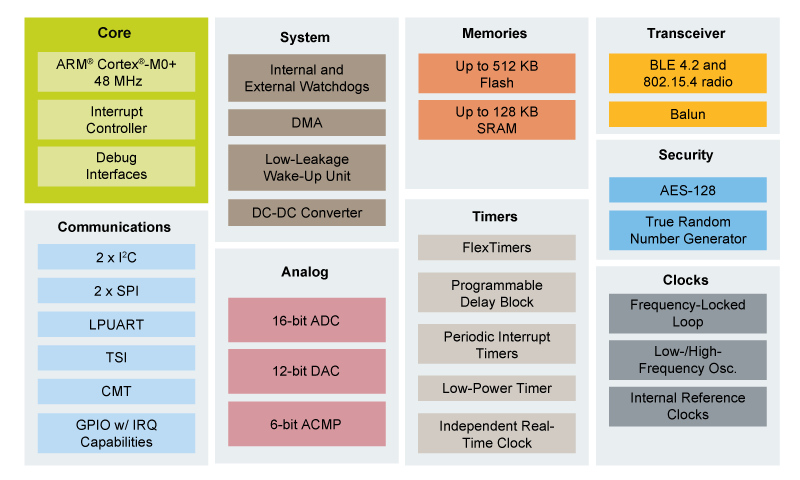
\includegraphics[width=\textwidth]{Figures/Hardware/KW41Z_block_diagram.jpg}
    \caption{Diagramme bloc interne du KW41Z}
    \label{fig-KW41Z_block_diagram}
\end{figure}

Une fois le microcontrôleur choisi, il était nécessaire de déterminer, les types d'interfaces allant être utilisées pour les différentes communications sur la DevBox. On peut voir sur \cref{fig-KW41Z_block_diagram} la présence de deux interfaces I2C, de deux SPI et d'une LPUART. Celle en UART a été réservée pour la communication entre le microcontrôleur Bluetooth et le coprocesseur LoRa. L'UART offre l'implémentation la plus versatile dans ce type de communication. Il peut y avoir des messages asynchrones provenant du coprocesseur selon le type de protocole de communication que l'utilisateur souhaite utiliser entre les deux éléments. Des interfaces SPI et I2C sont utilisées par les composants inclus sur la carte électronique. Cette même interface SPI est partagée avec un connecteur PMOD installé sur la DevBox. Une deuxième interface I2C est quant à elle réservée au port PMOD. Pour une vue d'ensemble des interfaces de communication et leurs connexions sur la carte DevBox, il est conseillé de visualiser le schéma Altium en \cref{AppendixDevBoxHardware}, sur le schéma nommé \texttt{Top View}.\\

\begin{figure}[ht!]
    \centering
    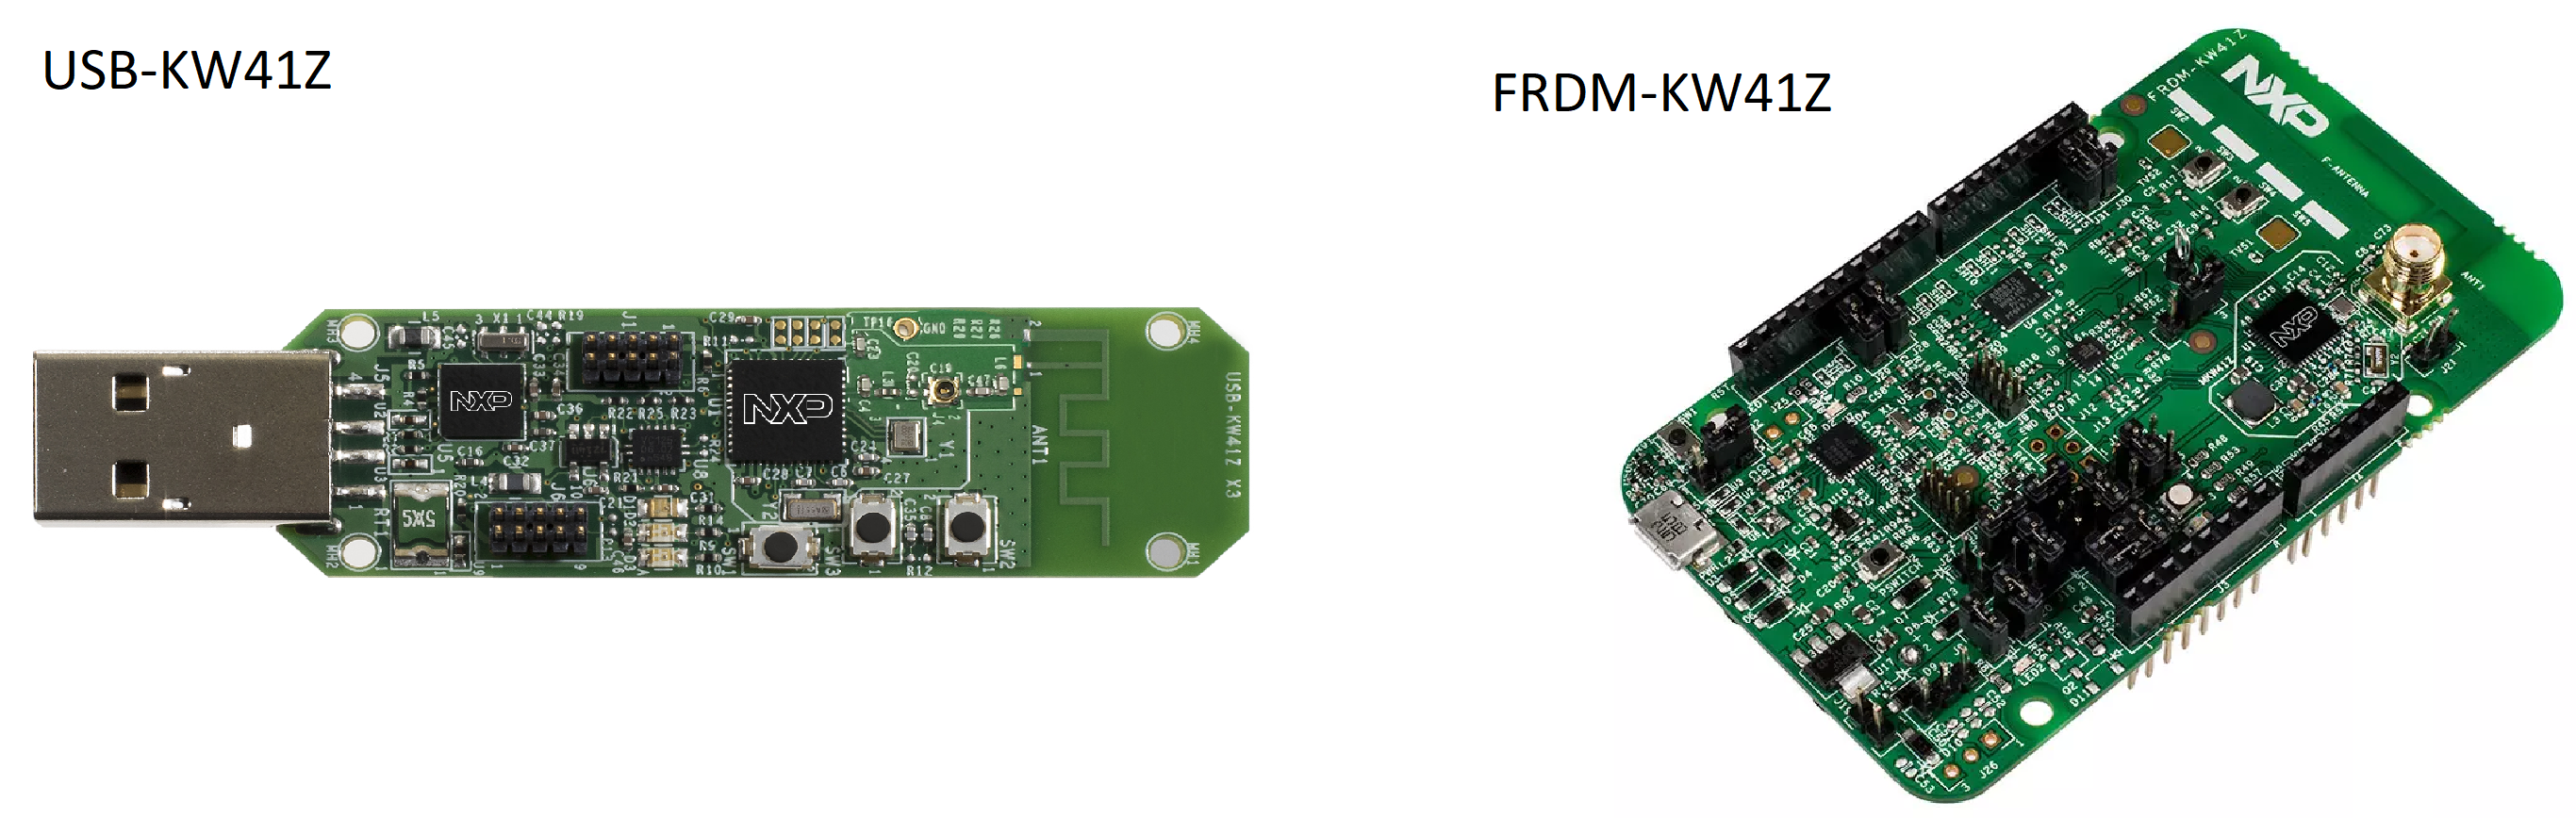
\includegraphics[width=\textwidth]{Figures/Hardware/nxp_dev_boards.png}
    \caption{Cartes de développement pour KW41Z}
    \label{fig-nxp_dev_boards}
\end{figure}

NXP propose deux cartes de développement avec le KW41Z visibles sur la \cref{fig-nxp_dev_boards}. La première est un simple dongle USB avec quelques boutons et une LED qui peut s'avérer utile pour faire des tests, par exemple, si on a besoin de scanner des paquets Bluetooth Low Energy. La FRDM-KW41Z est beaucoup plus complète. Elle propose en premier lieu des connecteurs compatibles avec les cartes d'extension Arduino. Elle contient en outre une meilleure antenne sur le PCB avec la possibilité de faciliter la connexion d'une antenne externe sur le connecteur prévu à cet effet. La carte est également équipée d'une vingtaine de \textit{jumpers} qui offrent la possibilité de tester les différents modes de consommation du circuit, ainsi que plusieurs confirmations des sorties. Elle possède également une mémoire flash externe qui peut être utilisée pour les mises à jour OTAA, ainsi qu'un accéléromètre/gyroscope via l'intégration d'un FXOS8700CQ. Cette deuxième carte a été utilisée dans le cadre de ce projet pour avoir une première approche avec les outils de programmation et ainsi pouvoir commencer à programmer parallèlement à la réalisation du PCB.


\FloatBarrier
\subsection{Gestion de la batterie}

Le système doit pouvoir être autonome. Afin de garantir cela, une batterie peut être connectée. La capacité de cette batterie reste au choix de l'utilisateur. 
L'utilisateur peut recharger celle-ci à l'aide d'un connecteur micro-USB présent sur la carte. L'aspect autonomie peut être encore plus poussé en connectant un panneau solaire directement sur la carte. Celui-ci a son propre connecteur dédié en entrée. Ce panneau permet ainsi de directement charger la batterie qui fournira à son tour la tension pour le système. 

Pour optimiser le rendement lors de l'utilisation d'un panneau solaire, un circuit intégré nommé BQ24210 \footnote{\url{http://www.ti.com/product/BQ24210}} a été utilisé. Ce dernier s'occupe directement de la recharge de la batterie supportant en entrée jusqu'à 20V de tension. Il est capable de fournir jusqu'à 800\,mA à la batterie, tout en protégeant celle-ci en cas de surtension. Il accepte également la possibilité de recharger avec une tension de 5V, permettant ainsi la recharge directement depuis une prise USB. \\


Une batterie est couplée au système. Celle-ci n'a pas de restriction de taille, elle doit simplement être de type Li-Ion en raison de la tension et de la courbe de charge fournie par le BQ24210. La batterie n'a pas besoin d'offrir un circuit de protection contre les surcharges ni les décharges profondes. Comme expliqué précédemment, le circuit BQ24210 interrompt la charge lorsque la batterie est pleine et protège la batterie des décharges profondes.  \\

L'ensemble de la carte est alimentée en 3.3V à l'aide d'un régulateur TPS62291. Celui-ci peut fournir un courant maximum de 1A. Ce haut courant est une précaution selon le type de cartes d'extensions que l'utilisateur souhaite ajouter à la DevBox. Il dispose d'un courant typique de fonctionnement très faible de 15 µA, pouvant ainsi consommer un minimum si l'on souhaite mettre toute la carte en basse consommation.

\FloatBarrier
\subsection{Coprocesseur LoRa}

La communication via LoRa est uniquement possible en utilisant les circuits proposés par l'entreprise Semtech, laquelle propose une gamme de circuits qui est visible à l'adresse suivante : 
\begin{center}
    \url{{http://www.semtech.com/wireless-rf/lora.html}}
\end{center}

Tous les circuits intégrés proposés sur le site de Semtech sont des périphériques qu'il faut ensuite relier avec un microcontrôleur via une communication SPI. Afin de pallier à cela, plusieurs fabricants ont développé des circuits intégrés composés d'un processeur couplé à un module de Semtech. Cela permet ainsi d'économiser du temps de conception. En effet, le plus difficile dans l'intégration de ces modules est la gestion de la partie radiofréquence. Celle-ci nécessite souvent des composants spécifiques qui supportent des fréquences plus élevées que des composants traditionnels. C'est le cas des condensateurs et inductances utilisées, ceux-ci devant être indiqués par le fabricant comme étant utilisables pour des fréquences supérieures à plusieurs gigahertz. Le plus souvent, les fabricants proposent des gammes complètes de ces composants pour ces cas d'utilisations, à l'instar des fabricants Murata\footnote{\url{https://www.murata.com/tool/netlist/mlcc}} ou Vishay\footnote{\url{https://www.vishay.com/capacitors/high-frequency/}}. \\

\begin{figure}[ht!]
    \centering
    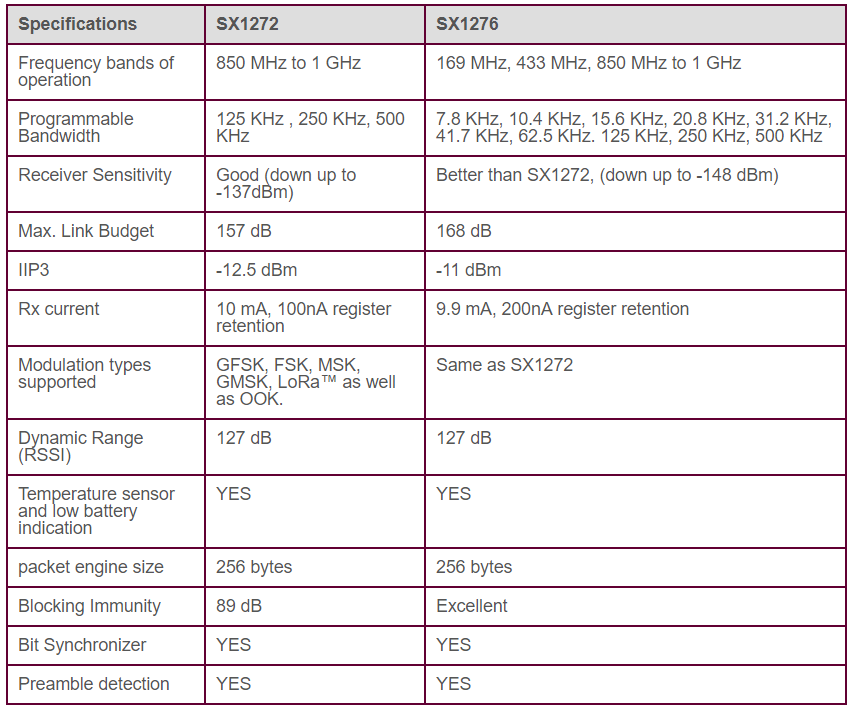
\includegraphics[width=0.9\textwidth]{Figures/Hardware/sx1272_vs_sx1276.PNG}
    \caption{Comparatif SX1272 et SX1276}
    \label{fig-sx1272_vs_sx1276}
\end{figure}

Tous les modules sont équipés d'un processeur connecté via SPI avec un circuit de Semtech. Parmi ces circuits se trouvent le SX1272 et le SX1276. Un comparatif sur le site \texttt{rfwireless-world}\footnote{\url{http://www.rfwireless-world.com/Terminology/SX1272-vs-SX1276-Semtech-LoRa-RF-Transceivers.html}} offre une vue d'ensemble des différences entre ces deux circuits. La \cref{fig-sx1272_vs_sx1276} illustre cette comparaison. Ils sont similaires, mais le SX1276 offre de meilleures performances. En effet, on constate que le SX1276 propose davantage de bandes fréquence ainsi qu'un meilleur \textit{link budget} (correspondant à la puissance de réception\footnote{\url{https://en.wikipedia.org/wiki/Link_budget}}). Le SX1272 ne propose que la fréquence 868 et 915 MHz de la bande de fréquence LoRa, soit celle respectivement pour l'Europe et l'Amérique du Nord respectivement. L'Asie avec ses 433 MHz n'est donc pas supportée. Le SX1276 est actuellement l'une des meilleures options disponibles par Semtech pour connecter un n\oe ud à un réseau LoRaWAN. Néanmoins, pour notre application, le SX1272 est parfaitement suffisant.\\

En termes de consommation, les deux circuits sont similaires. Preuve en est la comparaison des données présentes dans leurs \textit{datasheets} respectives (cf. \cref{fig-sx1272_78_current_consumption}). Dans le cadre d'applications low power, les consommations en veille et au repos sont les plus importantes. Celles-ci sont de 0.1 ou 0.2\,\si{\micro}A pour le mode \textit{sleep} et de 1.5\,\si{\micro}A pour le mode \textit{idle}. Ils constituent des circuits parfaits pour des applications basse consommation. Qui plus est, si on émet à la puissance maximale de 20 dBm, la consommation peut monter à 128 mA dans le cas du SX1272, constat qui doit être pris en compte lors du dimensionnement de l'alimentation du système.

\begin{figure}[ht!]
    \centering
    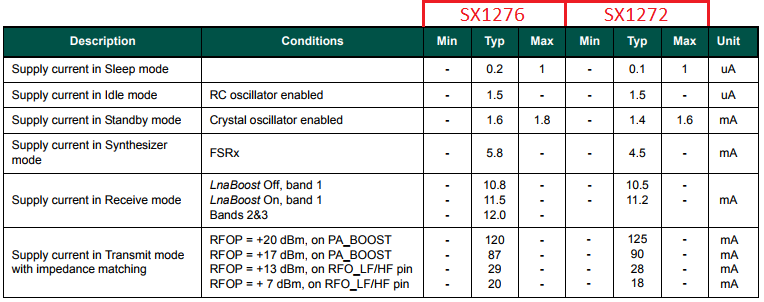
\includegraphics[width=0.9\textwidth]{Figures/Hardware/sx1272_78_current_consumption.PNG}
    \caption{Comparaison de la consommation de courant entre le sx1272 et sx1278}
    \label{fig-sx1272_78_current_consumption}
\end{figure}


\FloatBarrier
\subsubsection{Murata CMWX1ZZABZ-078}
\label{sec-hardware_lora_module}
\begin{figure}[ht!]
    \centering
    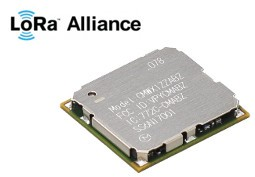
\includegraphics[width=0.4\textwidth]{Figures/Hardware/murata_module_image.jpg}
    \caption{Module LoRa CMWX1ZZABZ-078}
    \label{fig-murata_module_image}
\end{figure}

Le célèbre fabricant de semiconducteurs Murata\footnote{\url{https://www.murata.com/}} a commercialisé, en juillet 2016,  un module LoRa intégrant un SX1276, ainsi qu'un processeur de STMicroelectronics \cite{Muratala5:online}. Le module est visible sur la \cref{fig-murata_module_image}. Murata est renommé pour ses composants passifs de très haute précision, comme ses résistances, condensateurs ou inductances. Comme expliqué dans la section précédente, c'est toujours un challenge d'optimiser des circuits lorsque l'on utilise de hautes fréquences. Murata a développé ce circuit en y ajoutant ses composants afin d'offrir les meilleures performances en radio fréquence tout en minimisant l'espace occupé sur un PCB par le module.\\

\begin{figure}[ht!]
    \centering
    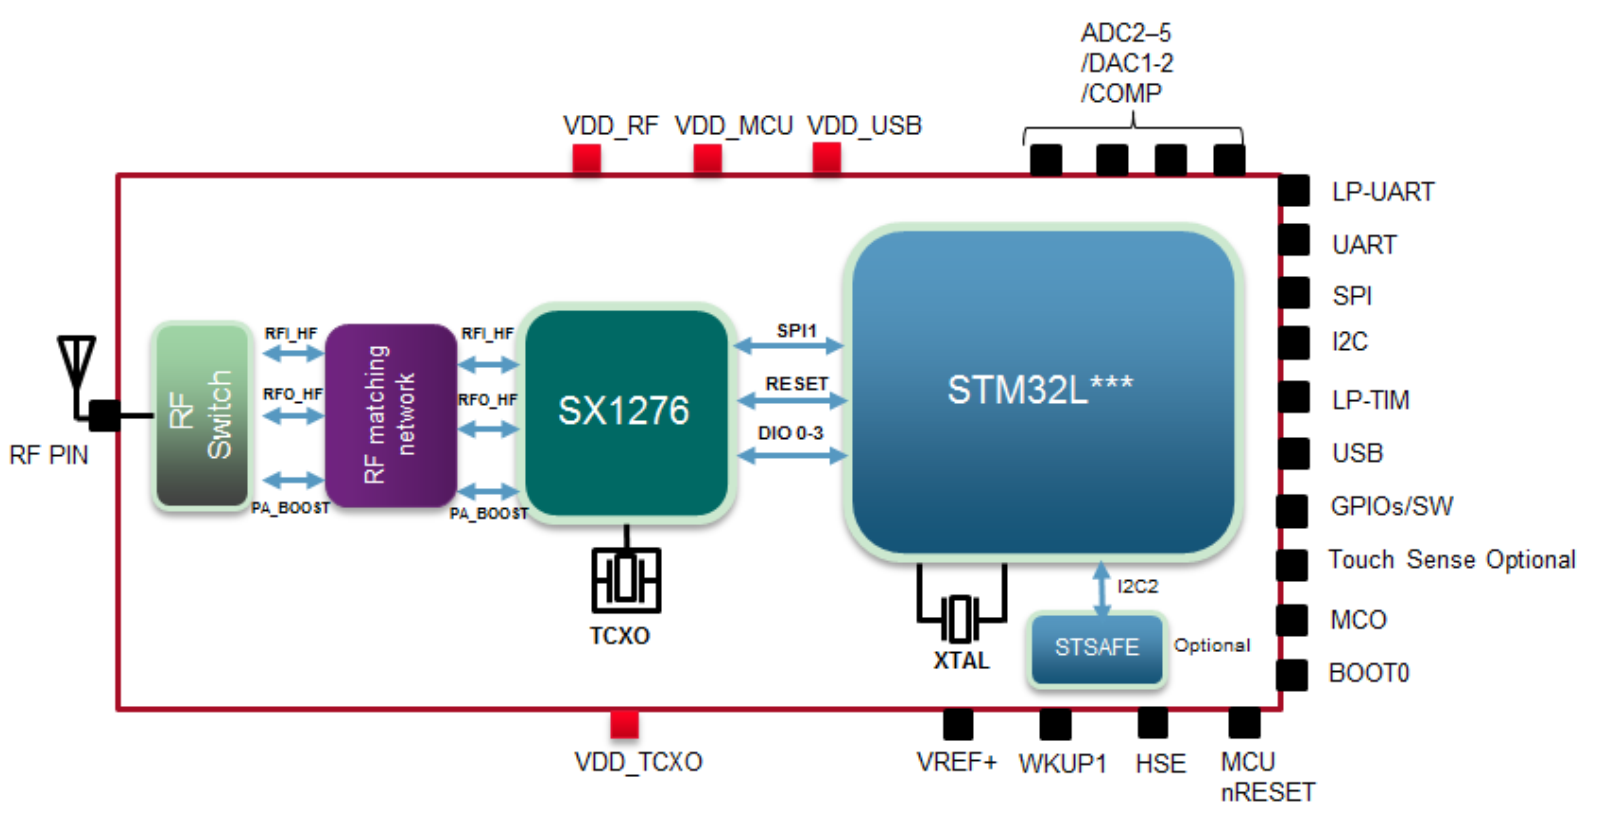
\includegraphics[width=0.9\textwidth]{Figures/Hardware/murata_bloc_diagram.PNG}
    \caption{Contenu du module LoRa CMWX1ZZABZ-078}
    \label{fig-murata_bloc_diagram}
\end{figure}

La \cref{fig-murata_bloc_diagram} illustre le contenu interne du module. On peut y voir un processeur ainsi que le SX1276. Le point fort de ce module est toutefois l'électronique placée entre le SX1276 et l'antenne. En effet, c'est la partie la plus difficile à réaliser lorsque l'on fait du routage haute fréquence, puisqu'il faut adapter les impédances et le dimensionnement des composants. Il existe en réalité deux modèles du CMWX1ZZABZ, la version 078 et la 091. La différence entre les deux est le processeur ST qui est placé en interne. Le 078 contient un STM32L082 alors que le 091 est équipé du STM32L072. C'est de là d'où proviennent les astérisques sur la \cref{fig-murata_bloc_diagram} avec le bloc bleu représentant le processeur. Cependant, à l'heure actuelle, le CMWX1ZZABZ-078 est le seul disponible sur le marché, aucun revendeur ne propose l'autre alternative. La \cref{fig-murata_bloc_diagram} nous indique également la présence d'un composant nommé \cref{sec-mcu_stsafe}. Son nom complet est \textit{State-of-the-art security for peripherals and IoT devices}. Celui-ci est développé par STMicroelectronics et propose plusieurs mécaniques d'authentification, afin de garantir que le périphérique fournissant des données à un client n'a pas été usurpé par une entité tierce. Ce périphérique est exploré plus en détail dans la \cref{sec-mcu_stsafe}.\\

Ses dimensions sont de 12.5\,mm x 11.6\,mm x 1.76\,mm; il est le plus petit des modules présentés ici. Ceci vient surtout du fait que Murata a utilisé sur son circuit des composants passifs avec des boitiers 0201 et 01005, ce qui lui a permis de créer le module le plus compact possible. C'est le seul des modules listé dans ce document qui propose un SX1276, contrairement à ses concurrents qui utilisent un SX1272. \\

La \textit{datasheet} du module ne spécifie pas toutes les consommations en courant. La \cref{fig-murata_current_consumption} contient le peux d'informations qui sont disponibles sur ses consommations. On y retrouve la consommation maximale du composant lors de l'émission à 20dBm. La \textit{datasheet} indique l'ajout de 3 mA en comparaison avec à la consommation seule du SX1276 (cf. \cref{fig-sx1272_78_current_consumption} pour les diverses consommations). Concernant la consommation en \textit{sleep}, on peut observer celle du STM32L082 pour avoir une idée, puisqu'aucune estimation n'est fournie par Murata. La \cref{fig-stm32L0_current_consumption} montre la consommation d'un STM32L082 en mode \textit{low power} avec tous les périphériques éteints. Ce mode serait envisageable avec la DevBox, car le microcontrôleur Bluetooth est capable d'activer ce mode à l'aide, par exemple, d'un GPIO. On observe des consommations très faibles en fonction des horloges choisies. Dans l'ensemble, la consommation du processeur varie de 4.7\,\si{\micro}A à 73\,\si{\micro}A selon la fréquence désirée et de la température d'opération. Il faut ensuite ajouter les consommations du SX1276 dans un mode similaire. Les consommations du SX1276 ont été précédemment présentées dans la \cref{fig-sx1272_78_current_consumption}, laquelle indiquait une consommation en mode \textit{sleep} de 0.2\,\si{\micro}A. Ce sont des courants tout à fait adaptés à des applications basse consommation. \\

\begin{figure}[ht!]
    \centering
    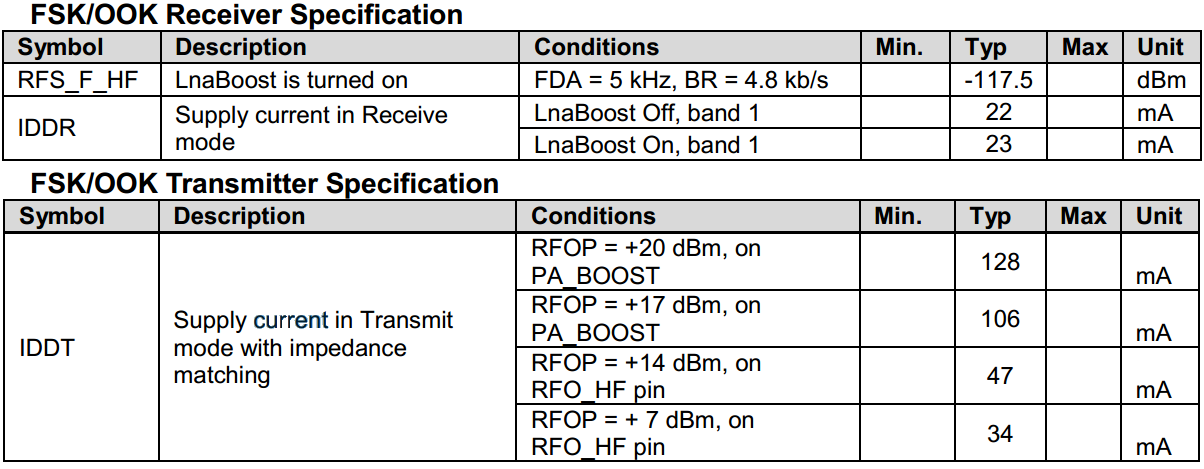
\includegraphics[width=0.9\textwidth]{Figures/Hardware/murata_current_consumption.PNG}
    \caption{Consommation en courant du module CMWX1ZZABZ-078}
    \label{fig-murata_current_consumption}
\end{figure}

\begin{figure}[ht!]
    \centering
    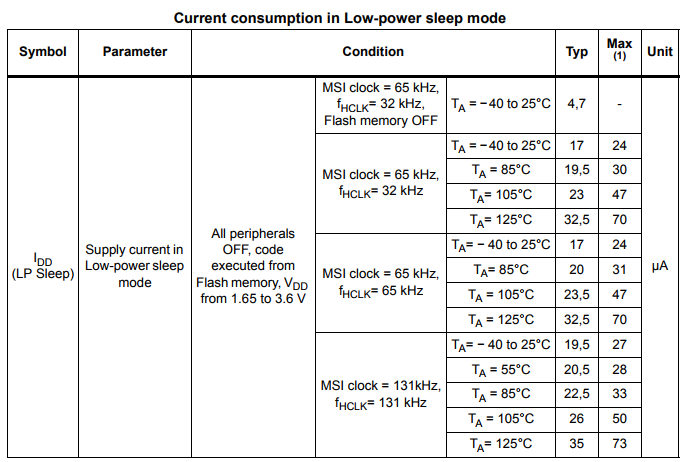
\includegraphics[width=0.9\textwidth]{Figures/Hardware/stm32L0_current_consumption.PNG}
    \caption{Consommation en courant du microcontrôleur STM32L082}
    \label{fig-stm32L0_current_consumption}
\end{figure}


\FloatBarrier
\subsubsection{IMST iM880B}

\begin{figure}[ht!]
    \centering
    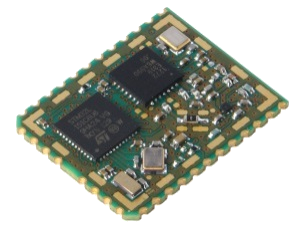
\includegraphics[width=0.7\textwidth/2]{Figures/Hardware/im880b-l_lora_module.png}
    \caption{Module LoRa iM880B du fabricant IMST}
    \label{fig-im880b-l_lora_module}
\end{figure}

Le module iM880B, visible sur la \cref{fig-im880b-l_lora_module}, est un produit de l'entreprise IMST. Celle-ci est renommée pour ses concentrateurs LoRa nommés iC880A\footnote{\url{https://wireless-solutions.de/products/radiomodules/ic880a.html}} qui, dotés d'un prix très accessible, facilitant la mise en place d'une gateway LoRaWAN. \\

Sa dimension étant de 25 x 20\,mm, il presque quatre fois plus grand que le module de Murata. Il dispose toutefois d'un processeur plus puissant que le Murata. En effet, il s'agit là de la gamme STM32L1, contrairement au STM32L0 du CMWX1ZZABZ. Le STM32L1 est basé sur un Cortex M3 cadencé à 16 MHz. Un processeur puissant n'a pas vraiment de sens dans ce projet, car le processeur LoRa restera le plus clair de son temps en veille en attendant des commandes du processeur principal.\\

\begin{figure}[ht!]
    \centering
    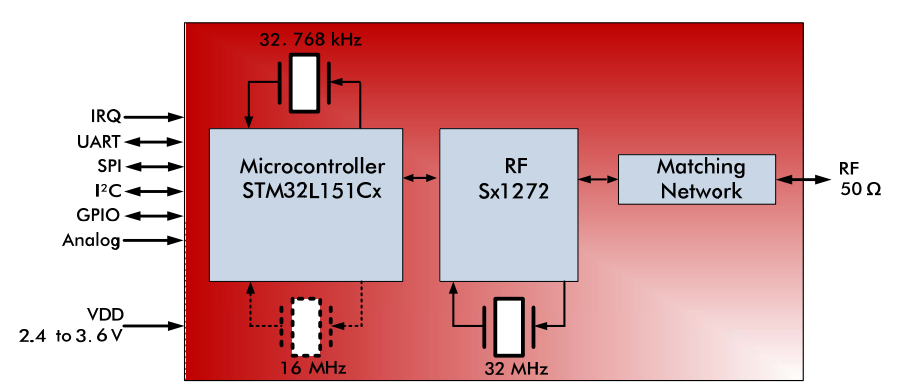
\includegraphics[width=0.7\textwidth]{Figures/Hardware/imst_bloc_diagram.PNG}
    \caption{Contenu du module LoRa iM880B}
    \label{fig-imst_bloc_diagram}
\end{figure}

La \textit{datasheet} de ce module nous fournit plus d'informations sur sa consommation. Les consommations sur les multiples modes sont visibles sur la \cref{fig-imst_current_consumption}. On a la même consommation en émission maximale que le Murata à 128 mA à +20 dBm. Cette \textit{datasheet}, présente cette fois la consommation lorsque le périphérique est en mode \textit{low power}. Celle-ci s'élève à 1.85\,\si{\micro}A avec un RTC activé, ou 800 nA sans celui-ci. La consommation du STM32L082 est donc similaire à celle du Murata. Malgré l'utilisation d'un processeur plus puissant (STM32L1), la consommation est donc inférieure à celle du CMWX1ZZABZ (4.9\,\si{\micro}A). Il faudrait examiner quel mode du microcontrôleur est activé dans cette configuration pour pouvoir faire une comparaison exacte entre les deux configurations. Dans le cas du Murata, il s'agissait du mode \textit{sleep} du processeur, mais cette information n'est pas disponible pour le module IMST.\\

\begin{figure}[ht!]
    \centering
    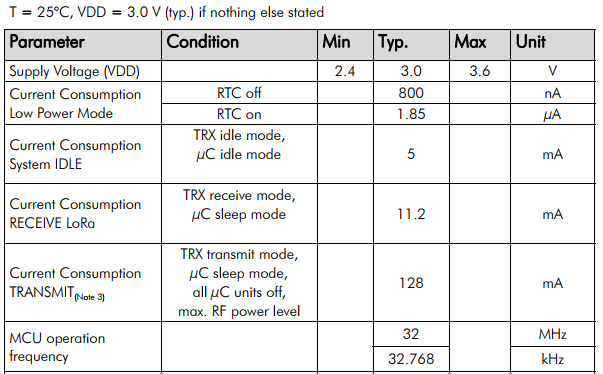
\includegraphics[width=0.7\textwidth]{Figures/Hardware/imst_current_consumption.PNG}
    \caption{Consommation en courant du module iM880B}
    \label{fig-imst_current_consumption}
\end{figure}

\FloatBarrier
\subsubsection{USI WM-SG-SM-42}

Le fabricant chinois USI a annoncé la production, en décembre 2016, d'un module similaire à celui de Murata. Celui-ci est nommé WM-SG-SM-42 et est visible sur la \cref{fig-usi_en.i-nucleo-lrwan1}. Celui-ci a été adopté par STMicroelectronics pour la création d'un \textit{shield} pouvant être placé sur des plateformes Arduino ou, directement, sur certaines de leur cartes de développement. Le contenu du module est illustré sur la \cref{fig-usi_bloc_diagram}.\\


\begin{figure}[ht!]
    \centering
    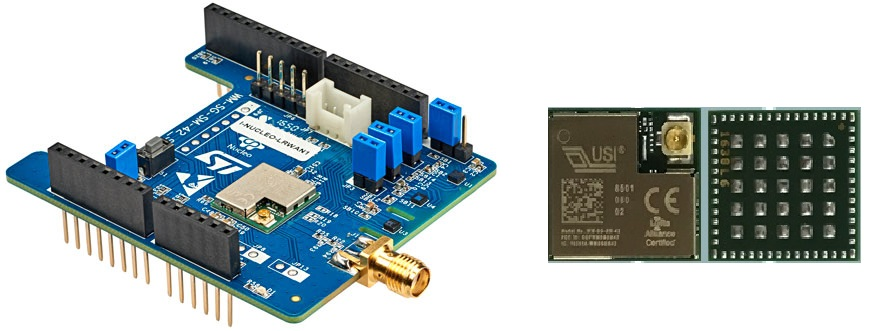
\includegraphics[width=0.75\textwidth]{Figures/Hardware/usi_i-nucleo-lrwan1.jpg}
    \caption{\textit{Shield} I-NUCLEO-LRWAN1 de ST et module USI WM-SG-SM-42}
    \label{fig-usi_en.i-nucleo-lrwan1}
\end{figure}

\begin{figure}[ht!]
    \centering
    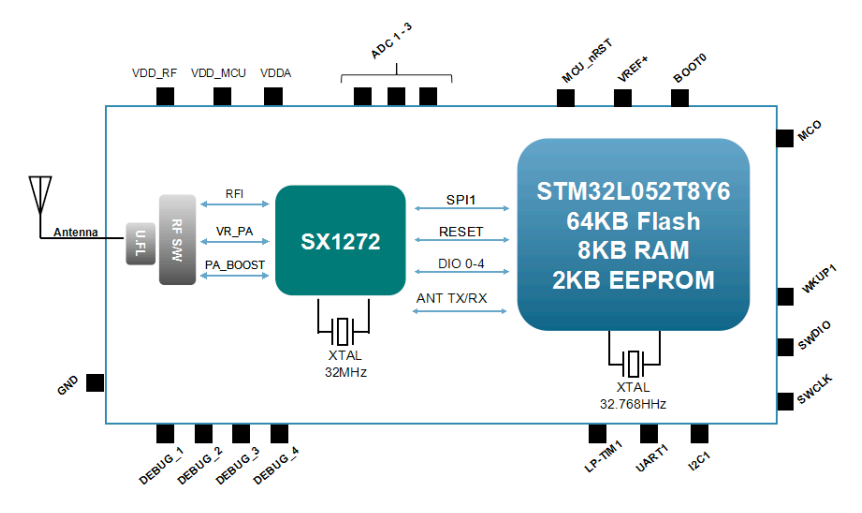
\includegraphics[width=0.8\textwidth]{Figures/Hardware/usi_bloc_diagram.PNG}
    \caption{Contenu du module WM-SG-SM-42}
    \label{fig-usi_bloc_diagram}
\end{figure}

Néanmoins, lorsque ce projet a commencé (septembre 2017), très peu d'informations étaient disponibles sur ce module, la seule référence postée sur le site du fabricant étant le communiqué de presse suivant : 
\begin{center}
    \url{http://www.usish.com/english/pressroom_more.php?n_sn=23}
\end{center}
Il n'y avait pas de description du produit ni de \textit{datasheet}, et le site n'était pas encore entièrement traduit en anglais. Il semble que tout cela se soit amélioré à la date de la rédaction de ce rapport (janvier 2018). Une page du produit est maintenant disponible\footnote{\url{http://www.usish.com/english/products_WM_SG_SM_42.php}}, de même qu’un PDF contenant une \textit{datasheet} du module\footnote{\url{http://www.usish.com/pdf/WM-SG-SM-42_Product\,\%20SPEC.pdf}}. Cependant, un problème majeur est toujours présent: ce module ne semble être disponible chez aucun revendeur; même sur des sites de vente en ligne comme Alibaba ou Aliexpress. Contrairement au module de Murata, qui est très facilement accessible. En revanche, le \textit{shield} produit par STMicroelectronics, équipé du module USI, est bien commercialisé en Europe et disponible chez plusieurs fournisseurs\footnote{\url{https://www.findchips.com/search/I-NUCLEO-LRWAN1}}.\\


Le module a une dimension de 12\,mm x 13\,mm, similaire au module de Murata. Il possède en outre un connecteur U.FL placé sur le module. Ceci est un avantage, puisqu'il permet d'économiser de la place sur le circuit si le but final est d'utiliser une antenne externe au PCB. Dans le cadre de ce projet, les deux options ont été retenues. L'utilisation de ce module aurait présenté un avantage en termes de gain de place. \\

\begin{figure}[ht!]
    \centering
    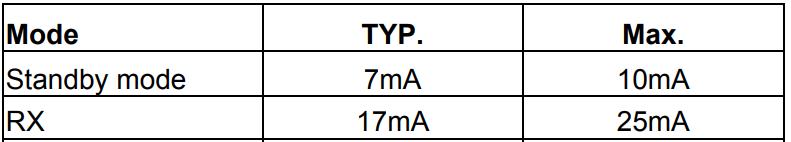
\includegraphics[width=0.7\textwidth]{Figures/Hardware/usi_current_consumption.PNG}
    \caption{Consommation en courant du module WM-SG-SM-42}
    \label{fig-usi_current_consumption}
\end{figure}

En ce qui concerne la consommation, la \textit{datasheet} reste très vague sur les informations. On peut voir uniquement les deux valeurs affichées sur la \cref{fig-usi_current_consumption} sur une configuration LoRa à 3.3V, 25°C et BW 125kHz. La consommation en mode \textit{standby} est trop élevée pour qu'elle soit celle de la consommation définitive du circuit. Il est possible de le mettre en mode \textit{low power}, mais la consommation de ce mode n'est pas documentée dans la \textit{datasheet}. Les consommations en émissions sont listées dans la \textit{datasheet} en fonction de la puissance d'émission. Elles varient de 47 mA à 126 mA à 868 MHz, avec des puissances d'émission allant de 5.6 à 19 dBm. Il faut être conscient que ces consommations ne sont présentes que lorsque l'utilisateur émet des paquets sur le réseau, sont durant quelques centaines de millisecondes au maximum. Pour la consommation en veille, on peut estimer que celle-ci est identique au Murata, puisque toute la gamme STM32L0 a des consommations similaires.\\

Comme pour les deux autres modules, la partie RF est intégrée dans le module, ce qui simplifie le développement matériel final. Il suffit de raccorder une antenne avec une impédance correcte de 50\,Ohms.

\subsubsection{Module choisi}

Le module de Murata est celui qui a été retenu pour ce projet. Il a l'avantage d'être extrêmement compact et simple à intégrer. Il est également disponible chez tous les revendeurs en Europe, contrairement à son rival, celui du fabricant USI. Au niveau logiciel, plusieurs codes exemples sont directement fournis par ST sur leur site Internet, ce qui offre un support en cas de problèmes au fil du développement.\\

\begin{figure}[ht!]
    \centering
    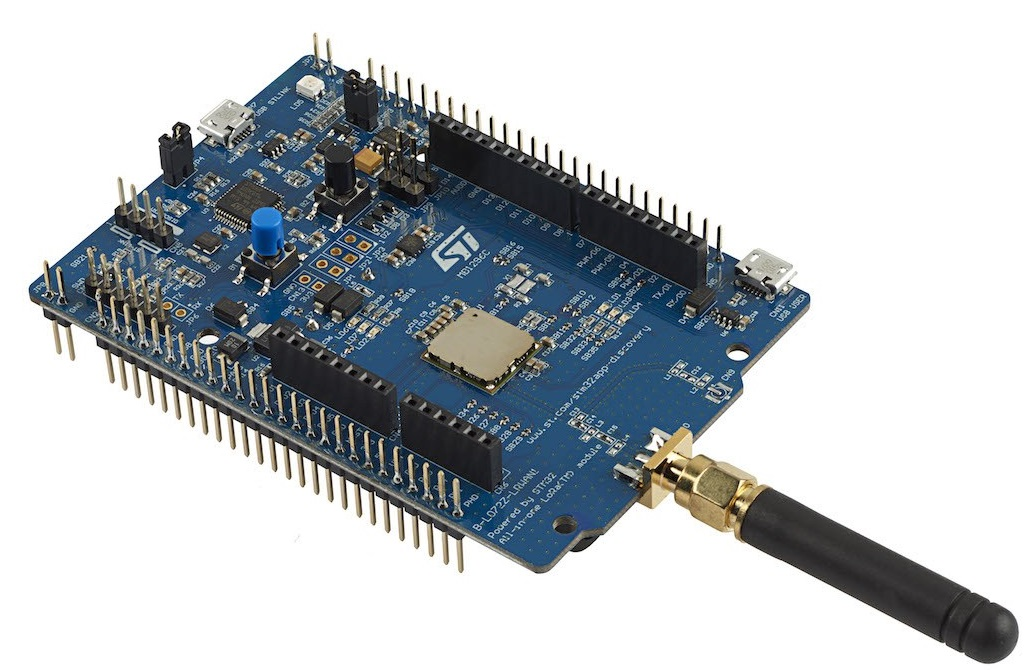
\includegraphics[width=0.6\textwidth]{Figures/Hardware/B_L072Z_st_dev_board.jpg}
    \caption{Carte de développement ST B-L072Z-LRWAN1}
    \label{fig-B_L072Z_st_dev_board}
\end{figure}

La carte de développement B-L072Z-LRWAN1 de ST Microelectronics, visible sur la \cref{fig-B_L072Z_st_dev_board}, offre la possibilité directement commencer à travailler sur le matériel sans que la carte électronique ne soit finalisée. Une partie du code de cette carte peut ensuite être facilement adapté sur la DevBox.



\subsection{Périphériques}

La carte DevBox est équipée de certains périphériques capteurs de données. Cette sous-section a pour but de les énumérer et de présenter leurs principales caractéristiques. Le schéma contenant ces périphériques est disponible dans l'\cref{AppendixDevBoxHardware} de ce document. Ils sont principalement présentés dans les schémas nommés \texttt{Embedded Sensors}, \texttt{GPS} et \texttt{PMOD}.

\subsubsection{LED}

Chaque microcontrôleur a à sa disposition quatre LED. Une bleu, une verte, une rouge ainsi qu'une jaune. Ces LED sont contrôlables via des GPIOs avec un état bas pour les allumer. Elles sont programmables selon la volonté de l'utilisateur.

\subsubsection{Buttons}

Chaque microcontrôleur a à sa disposition 2 boutons poussoirs. Ceux-ci produisent un état bas sur les GPIOs lorsque le bouton est pressé. Ces boutons sont programmables selon la volonté de l'utilisateur.

\subsubsection{Plateforme inertielle 9 axes}

\begin{figure}[ht!]
    \centering
    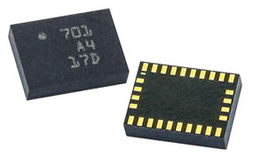
\includegraphics[width=0.35\textwidth]{Figures/Hardware/bno055_model.png}
    \caption{Plateforme 9 axes BNO055}
    \label{fig-bno055_model}
\end{figure}

La DevBox dispose d'une plateforme inertielle 9 axes (14-bit accéléromètre, 16-bit gyroscope et 16-bit magnétomètre) intégrés dans un même circuit électronique. Il s'agit du BNO055 fabriqué par Bosch Sensortec, visible sur la \cref{fig-bno055_model}, dont la communication s'effectue via un bus I2C relié au processeur principal (KW41Z). L'adresse I2C est configurable en fonction de l'état de la pin COM3 du module. Deux résistances (R11 et R13, une seule doit être placée) permettent de choisir le dernier bit de l'adresse. Si la résistance R11 est placée, le périphérique comporte alors l'adresse 0x29. Si c'est la résistance R13, cette adresse est 0x28. \\

À l'intérieur de ce composant, on trouve un ARM Cortex-M0+ avec un \textit{firmware} développé par Bosch, afin de pouvoir délocaliser le calcul de certaines données capturées. Cela permet, par exemple, de demander au composant de retourner la valeur de la gravité en $m/s^2$ ou de calculer de quaternions, réduisant ainsi le nombre d'opérations de lecture et surtout, économisant le temps de calcul du processeur principal sur un circuit embarqué. Le BNO055 a été créé avec la problématique de la consommation en tête. Dans son mode le plus bas, nommé \textit{Suspend Mode}, il ne consomme que 40 uA. \\

Bosch Sensortec propose un pilote pour la plupart de ses composants et celui-ci ne fait pas exception. Cela permet d'accélérer le développement, ce qui est parfait dans le cadre de ce projet, puisque l'utilisation de l'accéléromètre n'est pas l'objectif principal. \\


\subsubsection{Capteur environnemental et qualité de l'air ambiant}
\label{sec-hardware_bme680}

\begin{figure}[ht!]
    \centering
    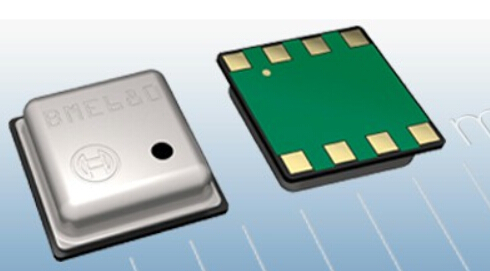
\includegraphics[width=0.35\textwidth]{Figures/Hardware/bme680_model.png}
    \caption{Capteur environnemental et qualité de l'air BME680}
    \label{fig-bme680_model}
\end{figure}

Un capteur de qualité de l'air a également été intégré sur la DevBox. Il s'agit du BME680 de Bosch Sensortec visible sur la \cref{fig-bme680_model}. Celui-ci ne mesure pas seulement la qualité de l'air, il mesure également la pression ambiante, la température, l'humidité et le gaz. Pour la mesure du gaz, il s'agit des \textit{Volatile Organic Compounds}\footnote{\url{https://en.wikipedia.org/wiki/Volatile_organic_compound}} (VOC), avec lesquels ont évalue la qualité globale de l'air ambiant. La liste des VOC utilisés pour l'index de la qualité de l'air ainsi que leur taux de précision est disponible sur la \cref{fig-bme680_voc_compounds}. Le capteur contient en interne une zone chauffante, laquelle s'active un bref instant pour pouvoir ensuite extraire la résistance de l'air. Cette résistance est la seule valeur fournie par ce capteur. Il faut ensuite faire des corrélations afin d'extraire les informations. La température, l'humidité et la pression sont elles directement retournées dans leurs unités respectives (°C, \,\% et Pa). 

\begin{figure}[ht!]
    \centering
    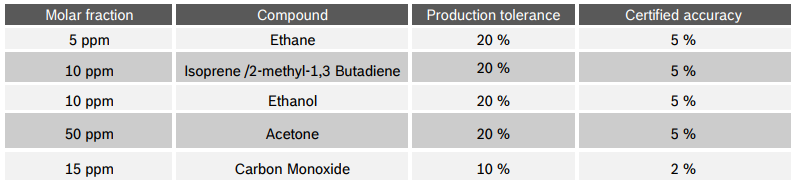
\includegraphics[width=0.8\textwidth]{Figures/Hardware/bme680_voc_compounds.png}
    \caption{VOC mesurés par le BME680}
    \label{fig-bme680_voc_compounds}
\end{figure}

Comme pour le BNO055, Bosch Sensortec met a disposition un driver en C\footnote{\url{https://github.com/BoschSensortec/BME680_driver}}. Le driver est beaucoup plus sommaire que celui du BNO055, car Bosch propose également une bibliothèque nommée BSEC pour \textit{Bosch Sensortec Environmental Cluster}\footnote{\url{https://www.bosch-sensortec.com/bst/products/all_products/bsec}}. Cette dernière n'est pas open source, il faut se contenter d'un binaire précompilé pour l'architecture utilisée. 


\subsubsection{GPS}
\label{sec-hardware_gps}

La DevBox peut également être équipée d'un GPS au besoin. Celui-ci étant assez couteux, il ne sera pas forcément monté sur toutes les cartes. Le GPS peut être utilisé si l'on souhaite traquer un objet en déplacement avec une très grande précision ($\pm$ 8m, 95\,\% du temps \cite{GPSgovGP89:online}). Il peut également être utilisé pour corréler la localisation obtenue via LoRa avec une position réelle. Cette géolocalisation par LoRa est expliquée dans l'introduction au LoRa de sous la \cref{sec_stateOfTheArtLoRa}.

\begin{figure}[ht!]
    \centering
    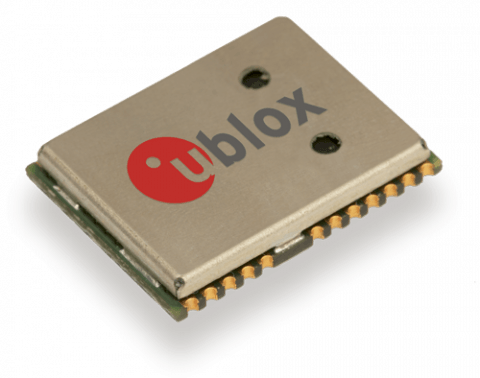
\includegraphics[width=0.35\textwidth]{Figures/Hardware/neo_3d_model.png}
    \caption{GPS U-blox NEO-M8}
    \label{fig-neo_3d_model}
\end{figure}

Le choix du GPS, a été opéré parmi ceux du fabricant suisse U-blox, spécialisé dans les semiconducteurs avec communication sans fil. Ils ont un large choix en termes de périphériques GPS. Ils proposent des GPS assortis d'antennes externes ou d'antennes céramiques placées directement sur un module. Ces GPS ont également la possibilité d'incorporer un \textit{low-noise amplifier} (LNA\footnote{\url{https://en.wikipedia.org/wiki/Low-noise_amplifier}}) pour l'amplification du signal. On peut également y trouver un filtre de type \textit{surface acoustic wave} (SAW\footnote{\url{https://www.vectron.com/products/saw/gps.htm}}) pour améliorer le signal et ainsi améliorer la réception. Lorsque ces deux éléments sont directement intégrés dans le module, cela facilite considérablement la complexité de routage d'un circuit équipé d'un GPS. En effet, s'il est nécessaire de créer ces deux éléments à l'extérieur du GPS, il faut faire particulièrement attention au type de composants utilisés, car le GPS communique à l'aide de deux hautes fréquences de 1575.42\,MHz et 1227.60\,MHz \cite{GPSsigna51:online}. Il y a également l'adaptation d'impédance sur la connexion avec l'antenne qui doit être correctement calculée en considérant l'épaisseur du circuit imprimé. \\

Le GPS recherché devait également être capable d'accepter la lecture par une interface de type I2C ou SPI, puisque ce sont les seules interfaces encore disponibles sur le KW41Z, puisque l'UART a été utilisé pour la communication entre le KW41Z et le module LoRa. Malheureusement, l'UART est l'interface la plus utilisée en GPS, donc certains GPS ne proposent que ce type de protocole de communication.

\begin{figure}[ht!]
    \centering
    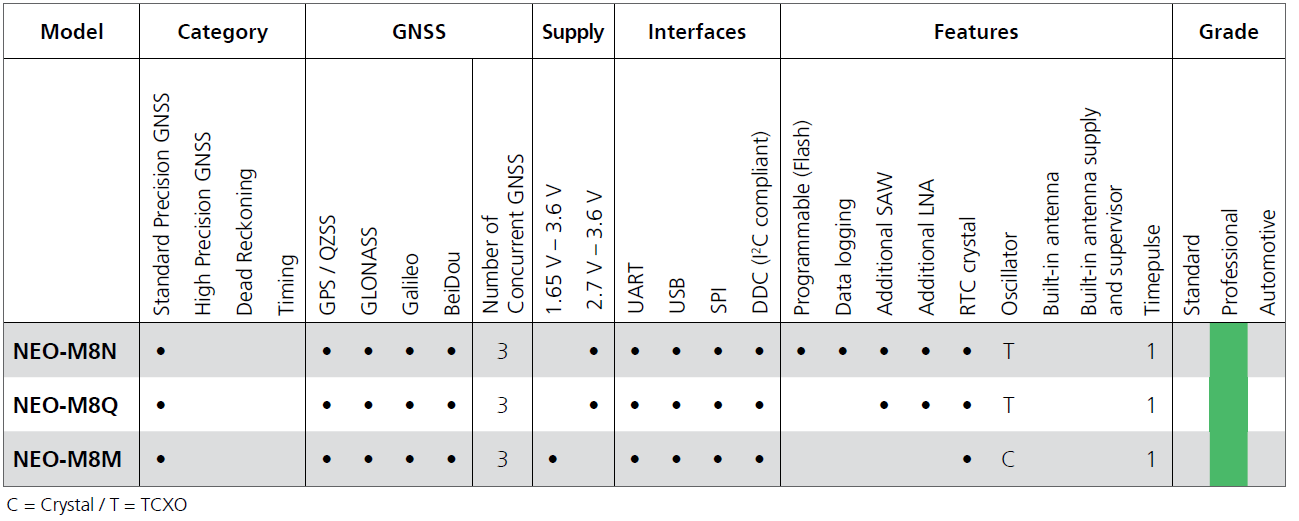
\includegraphics[width=0.95\textwidth]{Figures/Hardware/gps_neo_comparaison.png}
    \caption{Comparaison de la gamme de GPS U-blox NEO-M8}
    \label{fig-gps_neo_comparaison}
\end{figure}

Le GPS retenu a été le NEO-M8 dont la gamme complète est visible sur la \cref{fig-gps_neo_comparaison}. Celui-ci offre tout ce dont on a besoin, à savoir la possibilité d'une connexion avec une interface I2C ou SPI, ainsi que l'intégration d'un filtre SAW et d'un LNA. L'interface retenue pour le GPS a été le SPI, laquelle doit être partagée avec les composants qui sont connectés sur le connecteur PMOD (cf. \cref{sec-pmod_connector}). Sa taille est importante par rapport à celle des deux processeurs utilisés sur la carte (12.2 x 16 x 2.4\,mm pour le NEO-M8 contre 12 x 13\,mm pour le module LoRa). Il est entouré d'un boitier métallique, visible sur la \cref{fig-neo_3d_model}, afin d'atténuer les perturbations externes. Cependant, il ne nécessite aucun périphérique externe, à l'exception d'un connecteur U.FL pour la connexion d'une antenne externe.

\begin{figure}[ht!]
    \centering
    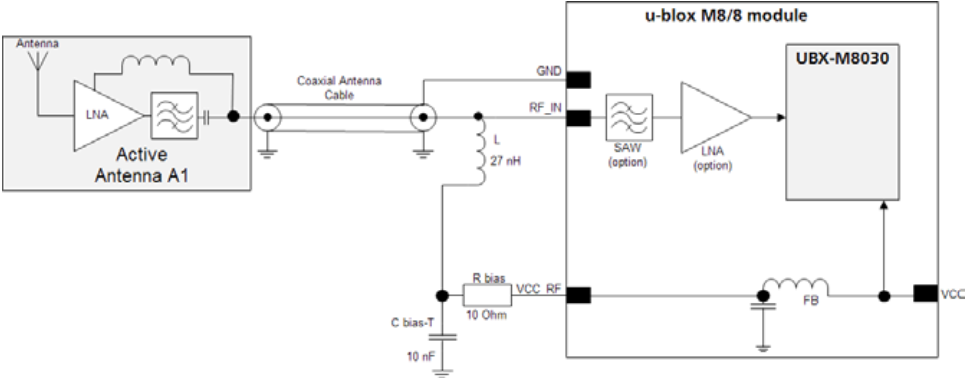
\includegraphics[width=0.9\textwidth]{Figures/Hardware/gps_neo_active_antenna.PNG}
    \caption{Schéma de connexion d'un NEO-M8 avec une antenne active}
    \label{fig-gps_neo_active_antenna}
\end{figure}

Le GPS a été routé sur la DevBox pour pouvoir utiliser des antennes non actives. Si l'utilisateur souhaite utiliser des antennes actives, il est possible de connecter l'alimentation directement le signal RF en entrée de l'antenne. Ceci n'est pas la connexion recommandée, mais elle est fonctionnelle. Selon la \textit{datasheet} du constructeur, si l'on souhaite convertir le signal RF actif, il faut normalement filtrer le signal d'alimentation afin d'éviter l'injection de bruit dans la radio. La \cref{fig-gps_neo_active_antenna} illustre la connexion recommandée par U-blox. Le NEO-M8 propose également une sortie nommée \textit{Timepulse} qui génère une pulse à chaque seconde (l'intervalle est configurable). Cette pulsation peut être utilisée pour synchroniser une horloge sur le microcontrôleur, de même que pour savoir si le GPS est prêt à fournir un nouveau paquet.\\

Ce module GPS entre directement dans la gamme professionnelle. La gamme supérieure est l'\textit{automotive} pour l'industrie des véhicules, mais il n'a pas été jugé nécessaire de prendre des composants de ce type pour le projet réalisé.
Le prix du GPS s'élève à 9.24 euros à partir de 250 pièces achetées (prix visible en janvier 2018).

\begin{figure}[ht!]
    \centering
    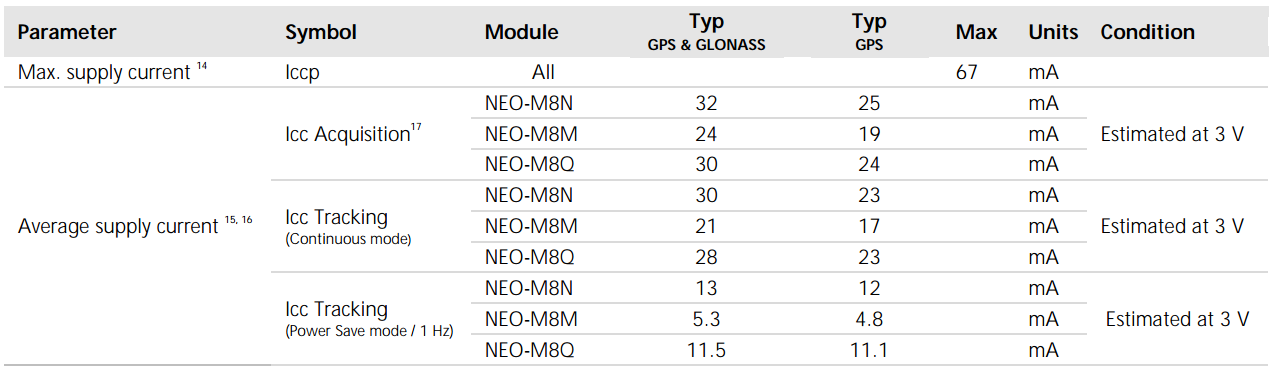
\includegraphics[width=0.95\textwidth]{Figures/Hardware/gps_neo_current_consumption.PNG}
    \caption{Consommation du GPS NEO-M8}
    \label{fig-gps_neo_current_consumption}
\end{figure}

En termes de consommation, tous les GPS sont de gourmands en énergie, car ils doivent continuer à écouter les signaux GPS. La \cref{fig-gps_neo_current_consumption} illustre combien le circuit consomme en acquisition. Cela dépend du mode choisi, le mode normal étant nommé \textit{ICC Acquisition}. Pour le NEO-M8Q, la consommation est en moyenne de 30mA avec GLONASS et GPS utilisés. À cette consommation, il faut encore ajouter celle d'une antenne active, dans la mesure où ce type d'antenne est raccordée. Les antennes actives consomment entre 3mA et 25mA selon les modèles utilisés. La consommation finale oscille ainsi autour de 50 mA, ce qui est problématique pour beaucoup de systèmes embarqués autonomes. Heureusement, le NEO-M8 peut être placé en mode \textit{low-power} via l'utilisation de commandes UBX; il est toutefois impossible de trouver la valeur exacte de la consommation de ce mode parmi les documents de U-blox. La seule référence à la consommation indique ce qui suit : 

\begin{quote}
\begin{center}
    \textit{During operation, the current drawn by the module can vary by some orders of magnitude, especially if enabling low-power operation modes.}
\end{center}
\end{quote}

Aucune valeur n'est fournie pour la consommation dans ce mode. Il est également possible de placer le GPS en mode \textit{backup}. C'est un mode où le GPS est désactivé, mais l'éphéméride des satellites est sauvegardée dans une mémoire volatile pour accélérer la synchronisation lorsque le mode normal est resélectionné. Pour sauver l'état de cette mémoire, une tension doit être appliquée au circuit sur une pin spécifique. Cette sauvegarde consomme 15\si{\micro{}}A si la tension de l'alimentation est de 1.8V. Ce type de mémoires peuvent être alimentées par des piles boutons, puisque le seuil minimum de tension est de 1.4V. Dans le cadre de ce projet, cette pin a été directement connectée à la tension VCC du circuit, celui-ci étant régulé par une batterie.


\subsubsection{Connecteur PMOD}
\label{sec-pmod_connector}

La carte DevBox est également compatible avec les connecteurs PMOD. Ces connecteurs sont basés sur un standard d'interface\footnote{\url{https://en.wikipedia.org/wiki/Pmod_Interface}} du même nom développé par l'entreprise Digilent\footnote{\url{http://store.digilentinc.com/}}. Le pinout des différents types d'interfaces est disponible sur la \cref{fig-pmod_type_pinout}. Dans le cas de la DevBox, les standards n'ont malheureusement pas pu être intégralement respectés, en raison de l'absence de GPIO disponibles sur le module Bluetooth. Les connecteurs sont compatibles avec les PMOD de type I2C, à l'exception des deux IO et des signaux. L'interface SPI est supportée à l'exception de INT et RST. Le pinout final de la DevBox est visible sur le schéma \texttt{PMOD} de l'\cref{AppendixDevBoxHardware}.\\

\begin{figure}[ht!]
    \centering
    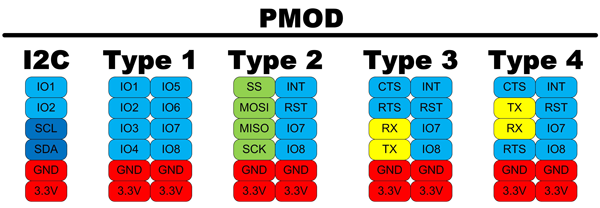
\includegraphics[width=0.7\textwidth]{Figures/Hardware/pmod_type_pinout.png}
    \caption{Pinout du standard PMOD en fonction des types choisis}
    \label{fig-pmod_type_pinout}
\end{figure}

Digilent commercialise des modules compatibles avec ces interfaces, ce qui facilite l'ajout d'un type de capteur qui n'aurait pas , par défaut, été rajouté sur la carte de développement. Le problème lié aux processeurs utilisés est le nombre de connexions disponibles vers l'extérieur. Nos deux microcontrôleurs ne sont équipés que de 48 pins au total, dont la moitié sont utilisés pour les alimentations et divers contrôles internes.

\FloatBarrier


\section{Schéma bloc général final}


La \cref{fig-hardware_bloc_diagram} illustre le schéma bloc final sur Altium de la carte DevBox. Il représente toutes les interfaces de communications entre les différents blocs. Cette image est également disponible sur l'\cref{AppendixDevBoxHardware}, tout comme les autres schémas électroniques du projet.\\


\begin{figure}[ht!]
    \centering
    \includegraphics[width=1.05\textwidth]{Figures/Hardware/hardware_bloc_diagram.png}
    \caption{Schéma bloc général de la DevBox}
    \label{fig-hardware_bloc_diagram}
\end{figure}


\FloatBarrier
\section{Réalisation et production du circuit électronique}

Le PCB réalisé a été routé selon les contraintes du fabricant de PCB\footnote{\url{https://www.pcbway.com/}} choisi, soit PcbWay. L'épaisseur choisie est de 1.6mm et les largeurs de piste minimales de 4mil. Les plus petits trous autorisés sont de 0.2mm. Afin de facilité la soudure, une finition à l'or a été demandée. Le temps de production est d'environ une semaine et demie à partir du moment où la transaction est validée. \\

Les composants électroniques ont principalement été commandés auprès de trois fournisseurs: Mouser, Farnell et Digikey. Mouser a été privilégié pour les composants, les deux autres n'ayant été utilisés qu'en cas de rupture de stock chez Mouser. La liste complète des composants avec leurs numéros de commande sont indiqués dans le projet Altium présent sur GitHub.\\

Un masque de dépose de pâte a dû être commandé à l'entreprise DB Products\footnote{\url{https://www.dbproducts.fr/}}. Une fois celui-ci reçu la production a pu être effectuée avec une machine de dépose de composants manuelle.

\section{Erreurs de conception et corrections possibles}
\label{sec_hardware_errors}

Une fois le PCB réalisé, plusieurs tests ont été effectués pour vérifier son fonctionnement. Quelques erreurs critiques ont du être corrigées : 

\begin{itemize}
    \item \textbf{Module LoRa} : VDD\_USB doit être connecté au 3.3V et non au 5V;
    \item \textbf{Module LoRa/Bluetooth} : RX et TX sont inversés sur la ligne UART;
    \item \textbf{Module LoRa} : VDD\_TCXO doit être connecté à la pin PA12 afin de pouvoir placer le SX1276 en mode \textit{sleep}.\\
\end{itemize}

Quelques améliorations peuvent également être envisagées pour la prochaine version, celles-ci n'étant toutefois pas un obstacle au fonctionnement de la version actuelle de la DevBox : 

\begin{itemize}
    \item \textbf{Module LoRa} : Connecter la mesure de la batterie (diviseur de tension) sur une pin ADC du module LoRa. Pour ce faire, il faut également relier la pin VREF à une référence externe ou au VCC. A l'heure actuelle, uniquement le KW41Z a accès à cette mesure.
    \item \textbf{GPS} : Ajouter le support d'une antenne active sur le PCB avec l'ajout de la tension d'alimentation filtrée sur le signal RF. Il est également possible d'ajouter un autre LNA à la sortie du signal RF (cf. \texttt{Hardware Integration} PDF aux pages 15 et 16). 
    \item \textbf{GPS} : Si l'on souhaite mettre en veille le GPS, il est possible de configurer une pin afin que celle-ci le place en mode \textit{sleep} lorsqu'elle est placée à un état 0. Il s'agit là de la pin EXTINT, mais celle-ci doit préalablement être programmée au moyen du protocole UBX.
    \item \textbf{GPS} : Connecter la pin GPS\_nCS sur une pin contrôlable par le DSPI en tant que \textit{chip select}. Actuellement, cette pin est contrôlée par un GPIO.
    \item \textbf{PCB layout} : Déplacer le bouton reset du KW41Z afin d'éviter les \textit{resets} non souhaités lors de la connexion sur câble JTAG. 
    \item \textbf{PCB layout} : Placer les boutons du KW41Z en face des LED du même microcontrôleur.
    \item \textbf{PCB layout} : Les LED de la charge de la batterie peuvent être placées sur le haut de la carte.
    \item \textbf{BME680} : Le BME680 pourrait être placé dans un coin plus proche du bord de la carte. On peut également découper un sillage autour du capteur afin de limiter la chauffe du PCB.
\end{itemize}

\section{Boitier en plastique}

\begin{figure}[ht!]
    \centering
    \includegraphics[width=0.6\textwidth]{Figures/Hardware/3d_case_devbox.png}
    \caption{Boitier imprimé en 3D pour y loger le circuit électronique}
    \label{fig-3d_case_devbox}
\end{figure}

Un petit boitier en plastique, visible sur la \cref{fig-3d_case_devbox}, a été créé afin d'y loger la carte. Ce boitier a été réalisé à l'aide du logiciel freecad\footnote{\url{https://www.freecadweb.org/}} et est cité dans les sources du projet sur GitHub. Son impression a été réalisée à l'aide d'une imprimante 3D.



\FloatBarrier


\chapter{Développement logiciel}

Ce chapitre a pour but d'expliquer l'implémentation logicielle sur les 3 plateformes utilisées (DevBox, Android et le serveur en Python). L'architecture générale y est présentée, mais également les implémentations spécifiques à chaque sous-catégorie.


\section{Architecture générale}

\begin{figure}[ht!]
    \centering
    \includegraphics[width=0.7\textwidth]{Figures/Software/diagram_project_software.pdf}
    \caption{Schéma général du projet avec les différentes technologies utilisées}
    \label{fig-diagram_project_software}
\end{figure}

L'architecture logicielle avec les différents protocoles de communications est visible sur la \cref{fig-diagram_project_software}. Au centre se situe la DevBox qui a deux interfaces de communication avec le LoRa et le Bluetooth Low Energy. Le Bluetooth sera accessible par une application développée pour Android dans un premier temps. La DevBox implémente une table GATT pour les services liés à la DevBox (batterie, LoRaWAN, GPS, BME680, etc. ). Ceux-ci sont explorés en détail en \cref{sec-BLEAllServices}.



\section{Scanneur de périphériques Bluetooth Low Energy}
\label{sec-software_scanner_ble}

L'implémentation du scanner de périphériques Bluetooth Low Energy est à cheval sur deux plateformes (Android et DevBox). Les spécifications liées à l'implémentation sur les plateformes sont présentées dans leurs sections respectives (\cref{sec-soft_devbox} et \cref{sec-soft_android}). \\


Les spécificités des \textit{advertisements} BLE ont été présentées dans l'état de l'art de ce document (\cref{sec-stateoftheart_ble}). Lorsqu'un périphérique Bluetooth Low Energy souhaite être visible, il doit diffuser un paquet de données. Ce paquet est entièrement personnalisable par l'utilisateur. Trois types de \textit{beacons} ont été présentés, parmi ceux-là, l'AltBeacon a été l'implémentation choisie. Principalement parce qu'elle est plus libre que le iBeacon. En effet, les \textit{Manufacturer ID} ne sont pas délivrés par une entité, contrairement aux iBeacons (si on souhaite être certifiée
par Apple). L'Eddystone est aussi très personnalisable, mais son grand avantage provient de ses URLs, qui dans notre projet ne sont pas nécessaires.  \\

Le \cref{tab-AltBeaconSmartCantonFormat} explique le contenu du format choisi pour diffuser la position. L'UUID de 16bit a un \textit{pattern} similaire à celui choisi pour les services Bluetooth. Ce qui est intéressant de voir c'est les bytes pour le Major et le Minor. Ceux-ci sont générés une seule fois aléatoirement pour chaque client au lancement du diffuseur d'\textit{advertisements}. Cela permet ainsi de traquer un utilisateur durant un laps de temps contrôlable, c'est-à-dire, tant que l'application n'est pas arrêtée sur le périphérique. L'adresse MAC du Bluetooth peut donc changer, mais on pourra suivre un utilisateur simplement en sauvegardant ce paquet.


\begin{table}[ht!]
\centering
\caption{Format du AltBeacon utilisé par le scanner Bluetooth}
\label{tab-AltBeaconSmartCantonFormat}
\begin{tabular}{|l|c|c|c|c|}
\hline
\multicolumn{5}{|c|}{\cellcolor[HTML]{BBDAFF}\textbf{AltBeacon Template}} \\ \hline
\textbf{Byte} & \textbf{0} & \textbf{1} & \textbf{2} & \textbf{3} \\ \hline
\textbf{0} & AD Length & AD Type & \multicolumn{2}{c|}{MFG ID} \\ \hline
\textbf{32} & \multicolumn{2}{c|}{BEACON Code} & \multicolumn{2}{c|}{BEACON ID} \\ \hline
\textbf{64} & \multicolumn{2}{c|}{BEACON ID} & \multicolumn{2}{c|}{BEACON ID} \\ \hline
\textbf{96} & \multicolumn{2}{c|}{BEACON ID} & \multicolumn{2}{c|}{BEACON ID} \\ \hline
\textbf{128} & \multicolumn{2}{c|}{BEACON ID} & \multicolumn{2}{c|}{BEACON ID} \\ \hline
\textbf{160} & \multicolumn{2}{c|}{BEACON ID} & \multicolumn{2}{c|}{BEACON ID} \\ \hline
\textbf{192} & \multicolumn{2}{c|}{BEACON ID} & RSSI TX & MFG RSV \\ \hhline{=====}
\multicolumn{5}{|c|}{\cellcolor[HTML]{BBDAFF}\textbf{AltBeacon SmartCanton}} \\ \hline
\textbf{Byte} & \textbf{0} & \textbf{1} & \textbf{2} & \textbf{3} \\ \hline
\textbf{0} & 0x1B & 0xFF & 0xFF & 0xFF \\ \hline
\textbf{32} & 0xBE & 0xAC & 0x00 & 0x00 \\ \hline
\textbf{64} & 0x00 & 0x00 & 0xAA & 0xAA \\ \hline
\textbf{96} & 0xBB & 0xBB & 0xCC & 0xCC \\ \hline
\textbf{128} & 0xDD & 0xDD & 0xDD & 0xDD \\ \hline
\textbf{160} & 0xDD & 0xDD & \multicolumn{2}{c|}{RANDOM} \\ \hline
\textbf{192} & \multicolumn{2}{c|}{RANDOM} & 0xBB & 0x00 \\ \hline
\end{tabular}
\end{table}


% ----------------------------------------------------------------- %
\FloatBarrier
\FloatBarrier
\newpage
\section{DevBox : module LoRaWAN}
\label{sec-soft_devbox}


Le module LoRaWAN est interconnecté avec le microcontrôleur Bluetooth via une interface UART. Le débit final de cette interface a été fixé à 115200 bits 
par seconde.

\subsection{Architecture logicielle}


STMicroelectronics propose une suite de bibliothèques pour ses divers microcontrôleurs afin de pouvoir communiquer avec des modules LoRa. Cette suite de bibliothèques est basée sur la très connue suite de développement STM32Cube\footnote{\url{http://www.st.com/en/embedded-software/stm32cube-mcu-packages.html}} et nommé \texttt{STM32 LoRa software expansion} \cite{STM32LoR36:online}. La \cref{fig-murata_lorawan_architecture} illustre l'architecture logicielle de cette suite de bibliothèques. Elle est composée d'un Hardware Abstraction Layer avec tous \textit{drivers} des périphériques du microcontrôleur STM32. Pour le \textit{middleware}, les blocs en vert sont repris de Semtech avec leur projet LoRaMac-node\footnote{\url{https://github.com/Lora-net/LoRaMac-node}}, alors que les blocs en bleu sont les \textit{drivers} fournis par ST. Il s'agit là de \textit{drivers} qui sont uniquement utilisés sur les différents capteurs présents sur les cartes de développement, telles que la B-L072Z-LRWAN1 et donc non utilisée dans ce projet. Il a un bloc nommé \textit{utilities}, créé par Semtech, mais modifié par ST. Cette modification permet d'utiliser au mieux les ressources matérielles du STM32L0, telles que les \textit{timers}, le mode \textit{Low-Power}, ainsi que le \textit{True Random Number Generator} (TRNG). L'architecture complète de cette suite de bibliothèques, ainsi que la description des diverses fonctions sont décrites dans le manuel d'utilisateur numéro \textbf{UM2073} de ST \cite{STM32LoR36:online}. 

\begin{figure}[ht!]
    \centering
    \includegraphics[width=0.8\textwidth]{Figures/Software/LoRaWAN/murata_lorawan_architecture.png}
    \caption{Architecture logicielle du CMWX1ZZABZ}
    \label{fig-murata_lorawan_architecture}
\end{figure}



\subsection{Exemples et modifications}
STMicroelectronics propose trois exemples de codes pour le CMWX1ZZABZ adaptés pour la carte de développement B-L072Z-LRWAN. Voici la description de ces projets : 
\begin{enumerate}
    \item \texttt{End Node} : projet ayant pour but de créer un n\oe ud LoRaWAN autonome avec la possibilité d'envoyer des données à des intervalles réguliers ou lors de la pression d'un bouton. 
    
    \item \texttt{AT Master} : offre la possibilité de communiquer avec un nouveau coprocesseur LoRa, implémentant un AT Slave interface. Cet exemple est très complet et est très utile pour comprendre comment la communication avec un AT Slave fonctionne. La \cref{fig-at_slave_master_connection} illustre la connexion entre un microcontrôleur utilisant l'interface \textit{Master} et un \textit{Slave}. Néanmoins, ce projet repose sur beaucoup de bibliothèques de ST, il est donc difficile de l'utiliser directement sur un microcontrôleur d'un autre fabricant.
    
    \item \texttt{AT Slave} : est utilisé pour offrir une interface de programmation du module à un utilisateur. Cet utilisateur peut utiliser un simple terminal série afin d'envoyer des commandes AT ou directement connecter un microcontrôleur (cf. \cref{fig-at_slave_master_connection}). La liste de toutes les commandes AT est disponible dans la note d'application nommée AN4967\footnote{\url{www.st.com/resource/en/application_note/dm00346311.pdf}}, avec les paramètres, ainsi que les réponses.
\end{enumerate}


\begin{figure}[ht!]
    \centering
    \includegraphics[width=0.7\textwidth]{Figures/Software/LoRaWAN/at_slave_master_connection.png}
    \caption{Connexion entre un AT \textit{Slave} et un AT \textit{Master} utilisant la suite de bibliothèque STM32Cube LoRa}
    \label{fig-at_slave_master_connection}
\end{figure}

Une interface entre le KW41Z et le CMWX1ZZABZ doit être implémentée, il a donc été décidé de reprendre le projet AT Slave pour le CMWX1ZZABZ et de l'adapter au besoin de la carte. Cet exemple implémente déjà toutes les opérations nécessaires pour rejoindre un réseau LoRa et envoyer des données. Le seul inconvénient de cette interface est l'utilisation d'un protocole basé sur des strings qui demande plus de stockage en mémoire et de temps pour transformer les requêtes. Mais le KW41Z a 128 kB de RAM, qui sont amplement suffisants pour cela. Toutefois, le code a dû être modifié avant d'enlever quelques périphériques qui ne sont pas présents sur la DevBox. Il faut également changer l'interface de communication afin d'utiliser l'UART0 de la carte qui n'est pas sur les mêmes pins que le LPUART initialement connecté.



\section{DevBox : NXP Kinetis KW41Z}

Le développement logiciel du microcontrôleur NXP Kinetis KW41Z est l'élément central de ce projet. Il implique l'interfaçage de divers périphériques avec plusieurs interfaces distinctes et tout cela sur un système temps réel.  

% ---------------------------------------------------------------------------------------------%
\subsection{\textit{OS Abstraction Layer} et \textit{Connectivity Framework}}
% ---------------------------------------------------------------------------------------------%

Les exemples de codes fournis par NXP pour ses microcontrôleurs implémentent tous FreeRTOS. Comme présenté en \cref{sec-RTOS_freertos}, il s'agit actuellement du RTOS le plus populaire et le plus actif en termes de communauté, ce qui apporte beaucoup d'avantages lors du développement. Lors de la présentation des différents RTOS, il a été fait référence aux couches d'abstraction de RTOS, en prenant l'exemple de l’OS Abstraction Layer (cf. \cref{sec-rtos_abstract_layer}). Celui-ci est visible sur la \cref{fig-freescale_osa_framework}. Il offre ainsi la possibilité de changer facilement de RTOS en fonction des besoins du projet pour les utilisateurs. NXP propose un framework nommé \textit{Connectivity Framework} qui s'occupe principalement des connexions avec le monde extérieur (Bluetooth, Wifi, etc.), mais également qui incluent différents autres blocs qui sont tous affichés sur la \cref{fig-freescale_osa_framework}. 

\begin{figure}[ht!]
    \centering
    \includegraphics[width=1.0\textwidth]{Figures/Software/freescale_osa_framework.PNG}
    \caption{\textit{Connectivity Framework} de Freescale (NXP)}
    \label{fig-freescale_osa_framework}
\end{figure}

Tout d'abord, en commençant par les différents blocs en bas de la \cref{fig-freescale_osa_framework} , la présence de plusieurs \textit{drivers} pour les périphériques peut être constatée. Ceux-ci couvrent toutes les interfaces de communications présentes sur les microcontrôleurs et sont tous très complets. On a ensuite la présence d'un RTOS qui est composé des différents composants standards d'un RTOS tel que des \textit{queues}, sémaphores et mutexes. Cette couche de RTOS repose directement sur l'interface matérielle, car il est parfois nécessaire d'adapter les drivers pour qu'ils soient \textit{thread safe} en fonction des différents ordonnancements utilisés par les RTOS et ainsi garantir l'intégrité des données. Vient ensuite l'interface OS Abstraction Layer pour uniformiser les différents RTOS. Un certain nombre de services sont disponibles, comme par exemple, le \textit{Serial Manager} qui a été utilisé dans ce projet pour gérer les connexions UART avec le coprocesseur LoRa. Celui-ci peut gérer des flux asynchrones provenant de plusieurs types d'interfaces (UART, USB, I2C et SPI). Pour les interfaces I2C ou SPI, celles-ci doivent être configurées avec une interruption sur un GPIO pour informer le \textit{Serial Manager }qu'une nouvelle donnée est disponible. La plupart de ces frameworks sont des tâches RTOS propre et utilisent des interfaces de communications \textit{thread-safe} afin d'être programmés.  \\

Ensuite, on peut voir l'élément qui simplifie l'intégration des communications externes (Bluetooth, WiFi, etc.) qui se nomme \textit{Components API}. Ce bloc a pour but de faciliter la programmation des diverses \textit{stacks} présentes sur les microcontrôleurs en fonctions des différentes gammes. On retrouve ainsi le Bluetooth, mais également des stacks pour le TCP/IP ou Thread. C'est souvent ce dernier bloc qui n'est pas open source. \\

\textit{Freescale Serial Communication Interface} (FSCI) est à la fois un module, mais également un protocole de communication utilisé entre les interfaces de communications externes (\textit{Components API}) et les services. On peut voir sur la \cref{fig-freescale_osa_framework} qu'il n'est pas forcément nécessaire de passer par le FSCI pour accéder aux composants depuis les composants applicatifs. Le FSCI ainsi que les \textit{frameworks} Services sont documentés dans un manuel de référence de NXP nommé \texttt{CONNFWKRM}. Toutefois, la documentation est légère, il est souvent plus facile de regarder le code source ou simplement les fichiers d'entêtes de fonctions pour les parties non open sources.

Le bloc, le plus haut niveau du framework, nommé \textit{upper layers}, est là où l'utilisateur doit normalement implémenter la plus grande partie de son code. Il a ensuite accès à ses trois interfaces pour utiliser toutes les ressources à sa disposition sur le microcontrôleur.


% ---------------------------------------------------------------------------------------------%
\FloatBarrier
\subsection{Interfaces de programmation}
% ---------------------------------------------------------------------------------------------%


\begin{figure}[ht!]
    \centering
    \includegraphics[width=0.6\textwidth]{Figures/Software/kw41z/board_paths.png}
    \caption{Bibliothèques et \textit{drivers} utilisés sur la DevBox}
    \label{fig-board_paths}
\end{figure}

Lors du développement de ce projet, plusieurs éléments ont été utilisés afin de simplifier la programmation de la DevBox. Un répertoire nommé \path{smartcanton_devbox_board} présent dans le dépôt GitHub au chemin d'accès, \path{dev/MKW41Z} contient des interfaces qui ont pour but d'être utilisées sur tous les projets qui utiliseront la DevBox à l'avenir. Ce répertoire est ensuite ajouté à l'aide d'un lien symbolique dans le projet MCUXpresso, comme illustré à l'aide de la \cref{fig-board_paths}. Certains de ces éléments sont des bibliothèques ou \textit{drivers} qui ont été développés par la communauté ou directement par les fabricants des composants électroniques utilisés.


\subsubsection{Bibliothèques et \textit{drivers} repris}

En plus du SDK fourni par NXP avec les différents \textit{drivers} pour le KW41Z, un certain nombre de bibliothèques ont été reprises et utilisées afin d'accélérer le développement du projet.

\subsubsubsection{AT Commander}
\label{sec-software_libs_atcommander}
La communication avec le module LoRaWAN s'effectue avec des commandes AT. Pour cela, une bibliothèque nommée AT Commander a été utilisée : 
\begin{center}
    \url{https://github.com/openxc/AT-commander}
\end{center}

Elle a toutefois du être modifiée à cause du format des requêtes qui sont transmissent par le module LoRaWAN. Cette bibliothèque est par défaut utilisable avec des modules AT de type RN42 ou XBEE, dont le format de trames diffère de celles du projet STM32 LoRa. Pour utiliser cette bibliothèque, l'utilisateur doit simplement spécifier deux fonctions pour lire et écrire sur un port UART souhaité. 

\subsubsubsection{minmea}
\label{sec-software_libs_minmea}

Le \textit{parsing} des trames GPS est fastidieux et peut être complexe en fonction des différents GPS et du type de données contenues dans une trame GPS. Il existe beaucoup de bibliothèques pour les GPS, mais souvent celles-ci ne sont pas adaptées aux systèmes embarqués. Cela s'explique par les fonctions de traitement de \textit{strings} qui demandent trop de ressources au processeur. Heureusement, il existe une bibliothèque nommée \texttt{minmea} qui implémente un parseur pour la spécification NMEA 0183 \cite{NMEA018318:online}. Celle-ci est pensée pour les environnements avec des capacités restreintes, comme les microcontrôleurs. Elle est disponible à l'adresse suivante :

\begin{center}
    \url{https://github.com/kosma/minmea}
\end{center}

\texttt{Minmea} est composée de deux fichiers et très simple d'utilisation. La trame récupérée depuis le GPS lui est directement fournie et celle-ci s'occupe d'extraire toutes les informations souhaitées. Elle supporte les données de type RMC, GGA, GSA, GLL, GST, GSV, VTG et ZDA \cite{NMEAdata3:online}. Toutes les données sont ensuite accessibles via des structures selon le type de données.

\subsubsubsection{BNO055 \textit{driver}}
\label{sec-softwaire_driver_bno}

Bosch Sensortec fournit différents drivers pour la plupart de ses composants. Un \textit{driver} est disponible pour le BNO055, avec lesquels, il est possible de communiquer en I2C ou SPI. Selon le mode choisi, des fonctions pour la lecture et écriture doivent être fournies à la bibliothèque. L'utilisateur peut ensuite accéder aux différents registres du capteur.
Le code source de la bibliothèque contient plus de 17000 lignes de codes, car le BNO055 est un capteur à la fois complet, mais également complexe à programmer. Ce \textit{driver} est disponible à l'adresse suivante : 
\begin{center}
    \url{https://github.com/BoschSensortec/BNO055_driver}
\end{center}

\subsubsubsection{BME680 \textit{driver}}
\label{sec-softwaire_driver_bme680}

Le BME680 dispose également d'un driver pour récupérer les différentes informations du capteur comme pour le BNO055. Cependant, une grande partie de la correction des mesures s'effectue en logiciel, ce qui a pour conséquence de créer un \textit{driver} minimal. Il est capable de fournir uniquement la valeur brute de la température, de l'humidité et de la pression. Pour la mesure de la qualité de l'air, celle-ci est uniquement possible à l'aide d'un traitement logiciel. La seule information sur le gaz est la valeur ohmique, mais cela n'indique en rien la qualité de l'air. La bibliothèque est disponible sur le dépôt GitHub suivant : 
\begin{center}
    \url{https://github.com/BoschSensortec/BME680_driver}
\end{center}

\subsubsubsection{Bosch Sensortec Environmental Cluster}
\label{sec-software_bme680_bsec}

Comme expliqué dans la section précédente, ainsi qu'en \cref{sec-hardware_bme680}, la grande partie du traitement des données s'effectue en software. Le fabricant propose une bibliothèque nommée Bosch Sensortec Environmental Cluster (BSEC). BSEC n'est pas open source, elle est fournie précompilée pour diverses architectures, limitant le débogage du système, mais permettant ainsi de garder secret l'algorithme utilisé. La bibliothèque à l'adresse suivante :

\begin{center}
    \url{https://www.bosch-sensortec.com/bst/products/all_products/bsec}
\end{center}


\begin{figure}[ht!]
    \centering
    \includegraphics[width=0.8\textwidth]{Figures/Software/kw41z/bme680_iaq_indexes.PNG}
    \caption{Niveaux de l'indice IAQ}
    \label{fig-bme680_iaq_indexes}
\end{figure}

\begin{figure}[ht!]
    \centering
    \includegraphics[width=0.8\textwidth]{Figures/Software/kw41z/iaq_accuracy.PNG}
    \caption{Niveaux de l'indice IAQ Accuracy}
    \label{fig-iaq_accuracy}
\end{figure}

Pour utiliser cette bibliothèque, le \textit{driver} BME680 doit être également utilisé et lié au projet. La qualité de l'air est mise à disposition à l'aide de l'indicateur \textit{Indoor Air Quality} (IAQ). Celle-ci est accompagnée d'un niveau de fiabilité nommé IAQ \textit{Accuracy}. L'IAQ est calculé à l'aide d'un algorithme propriétaire dont la valeur finale se situe entre 0 et 500. Les différents paliers de cet indice sont visibles sur la \cref{fig-bme680_iaq_indexes}. Selon le guide d'intégration de la bibliothèque BSEC \cite{BSEClib:online}, le périphérique nécessite 4 à 28 jours de calibration. Sur cette période, le composant doit être exposé 30min au milieu le moins pollué possible et 30min dans un milieu très pollué, afin de permettre une calibration plus correcte. La température et l'humidité sont également corrigées en fonction de l'environnement et la bibliothèque offre même la possibilité de placer un offset sur les valeurs pour prendre en compte l'échauffement des composants électroniques à proximité.



\subsubsection{Bibliothèques et \textit{drivers} développés}

Tous les fichiers présents sur la \cref{fig-board_paths} illustrant le répertoire \texttt{board} qui ne sont pas dans un sous répertoire ont été développés pour ce projet. Les sous-sections qui suivent ont pour but d'expliquer l'utilité des fichiers les plus importants. 


\subsubsubsection{\texttt{pin\_mux}}

\begin{figure}[ht!]
    \centering
    \includegraphics[width=1.0\textwidth]{Figures/Software/kw41z/mcuxpresso_pin_tools.PNG}
    \caption{Utilitaire de configuration du multiplexeur de pins des microcontrôleurs NXP}
    \label{fig-mcuxpresso_pin_tools}
\end{figure}


Le KW41Z est équipé d'un multiplexeur de pins, cela signifie que chaque pin peut avoir plusieurs rôles qui peuvent se modifier en cours d'exécutions. Pour aider les programmeurs, NXP propose dans le cadre de son SDK, un utilitaire nommé MCUXpresso Config Tools \footnote{\url{https://mcuxpresso.nxp.com/en/pins}}. Cet utilitaire est visible sur la \cref{fig-mcuxpresso_pin_tools}. Une fois les pins connectés sur l'utilitaire, il est possible d'exporter la configuration sous forme de fichier source afin d'être intégré au projet.


\subsubsubsection{\texttt{board}}

Une partie de ces deux fichiers est une reprise des divers exemples prodigués par NXP. Leur rôle est de fournir des accès génériques sans tenir compte du pinout appliqué au microcontrôleur. Par exemple, on peut y trouver une fonction nommée \path{BOARD_EnterLowPowerCb} offrant ainsi la possibilité de mettre le processeur en mode basse consommation. 


\subsubsubsection{\texttt{bme680 et bno055 support}}

Les drivers et bibliothèques du BME680 et BNO055 sont très bien fournis (cf. \cref{sec-softwaire_driver_bno} et \cref{sec-softwaire_driver_bme680}), mais il faut leur spécifier les interfaces matérielles qui communiquent avec le périphérique. Dans les deux cas, il s'agit d'un BUS I2C. Pour éviter tout problème de concurrence entre les tâches qui utilisent la même interface, le driver \path{fsl_i2c_freertos} a été utilisé dans ces deux bibliothèques. \\


La bibliothèque BSEC enregistre ponctuellement l'état de son algorithme d'apprentissage. Pour cela, il est nécessaire de fournir une fonction de sauvegarde en mémoire non volatile. Un secteur en flash a donc été réservé pour sauvegarder toutes les 2 heures l'état de la bibliothèque (fréquence de sauvegarde configurable). Une fonction de relecture de cette mémoire est également nécessaire, ainsi qu'une fonction pour la configuration utilisée (cf. le document \textit{Integration Guide
Bosch Software Environmental Cluster} (BSEC) \cite{BSEClib:online} pour toutes les configurations possibles). \\

Dans le cas du BME680, une fonction nommée \path{bme680_bsec_kw41z_iot_loop} s'occupe de réaliser l'acquisition en continu du capteur avec toute la gestion de la bibliothèque BSEC (capture, attente, sauvegarde de l'état de l'algorithme, etc.). L'utilisateur doit simplement fournir une fonction de \textit{callback} afin d'être notifié de la mesure d'un nouveau set de données, ainsi que divers paramètres concernant cette fréquence d'acquisition.

\subsubsubsection{\texttt{lorawan\_controller}}
\label{sec-softawre_kw41z_libs_lorawan_controller}

Le contrôleur LoRaWAN est l'un des éléments centraux de ce travail, c'est grâce à celui-ci qu'il est possible de configurer et de communiquer à travers un réseau LoRaWAN. Pour la communication avec le module LoRaWAN, les commandes AT sont envoyées à l'aide de la bibliothèque AT Commander (cf. \cref{sec-software_libs_atcommander}). Le contrôleur supervise également un espace mémoire en flash afin de stocker la configuration du module LoRaWAN dans but de se reconnecter au réseau lorsque le processeur est redémarré. Le contrôleur stocke en interne la configuration appliquée au module, ainsi que la nouvelle configuration que l'utilisateur souhaite appliquer à celui-ci. La structure \path{lorawanControllerConfiguration_t} a pour but de contenir toutes les informations de la configuration du module. À l'heure actuelle, l'AppKey est stockée sur le KW41Z, mais dans une version finale du système, celle-ci doit être stockée directement dans le module pour éviter que quelqu'un ne puisse intercepter la configuration lors de l'initialisation. Les attributs de cette structure sont listés ci-dessous :



\begin{tcolorbox}
  [top=-1mm, bottom=-3mm, left=0mm, right=0mm, enhanced,breakable,
  attach boxed title to top center={yshift=-3mm,yshifttext=-1mm},colback=LightGray,colframe=DarkGray,
  colbacktitle=DarkGray, fonttitle=\footnotesize\bfseries,boxed title style={size=small,colframe=DarkGray},
  title=\path{lorawan_controller.h} ]


\inputminted[firstline=30,lastline=54,bgcolor=LightGray,fontsize=\tiny,breaklines,linenos]{C}{SourceCode/lorawan_controller.h}
\end{tcolorbox}

Ces champs sont stockés sous forme de chaine de caractères. Cela est dû au fait que la communication avec le module LoRaWAN est basée sur des commandes AT, et donc les paramètres de ces commandes sont tous des \textit{strings}. Afin d'économiser du temps CPU dans la conversion des données lors de l'envoi de chaque commande au module, il a été décidé de garder ce format tout au long du processus, au risque d'occuper plus d'espace mémoire. Un CRC codé sur 16bits a été ajouté à la configuration, à la suite de plusieurs problèmes liés à l'écriture et à la lecture de la mémoire flash. Ces problèmes ont été résolus, mais ce CRC a été maintenu puisque si la carte s'éteint lors de l'écriture en flash, les données peuvent toujours être corrompues. Si le CRC est erroné lors de la lecture d'une configuration, la configuration par défaut est appliquée. 

\begin{figure}[ht!]
    \centering
    \includegraphics[width=0.8\textwidth]{Figures/Software/diagram_lorawan_init_module.pdf}
    \caption{Diagramme de la fonction d'initialisation du module LoRaWAN}
    \label{fig-diagram_lorawan_init_module}
\end{figure}

L'une des étapes les plus importantes du module est son initialisation. L'initialisation s'effectue à l'aide de la fonction \path{lorawan_controller_init_module}. Un diagramme représentant l'algorithme utilisé est visible sur la \cref{fig-diagram_lorawan_init_module}. En observant ce diagramme, on constate que la configuration du module est sauvegardée uniquement lorsque le réseau a pu être correctement rejoint à l'aide d'un \textit{Join Request}. Tant que la demande de \textit{join} n'est pas confirmée, le contrôleur est bloqué. Un temps d'attente maximum est configurable dans le contrôleur en spécifiant le nombre de vérifications du statut de \textit{join} avec le temps d'attente entre chacune de ces vérifications.

\subsubsubsection{\texttt{neo-m8}}
 \label{sec-software_libs_neom8}

Ces fichiers contiennent toutes les fonctions pour récupérer les données provenant du NEO M8 avec le support de l'interruption du signal \texttt{timepulse} pour démarrer l'acquisition. Une fois les données récupérées, il est possible de spécifier une fonction de \textit{callback} à l'aide d'un pointeur pour informer l'application de la réception de nouvelles mesures. Ces mesures sont ensuite accessibles par l'application en utilisant le parseur minmea (cf. \cref{sec-software_libs_minmea}). Cette bibliothèque est principalement utilisée par la tâche GPS présentée en \cref{sec-software_kw41z_algo_gps}.\\


Le NEO M8 supporte le protocole propriétaire UBX afin de communiquer avec le GPS pour le configurer. Cette configuration n'a pas été mise en place à l'heure actuelle, principalement par manque de temps. Toutefois, si l'on souhaite avoir un système base consommation, le support de ce protocole doit être fait. Plusieurs bibliothèques sont disponibles pour le protocole UBX\footnote{\url{https://github.com/arobenko/ublox}}, cependant peu d'entre elles sont orientées systèmes embarqués avec de faibles ressources. Le protocole UBX est très conséquent et nécessite beaucoup de place en mémoire. Par défaut le GPS envoie des trames GPS NMEA avec un intervalle de 1 seconde et sans la possibilité d'être mis en mode \textit{sleep}. Ces paramètres sont uniquement modifiables à l'aide du protocole UBX.

\subsubsubsection{\texttt{string\_utils}}

Dans ce projet, il est souvent nécessaire de faire des conversions entre plusieurs formats de données. Le type de conversion le plus utilisé est le tableau de \textit{bytes} en \textit{string} et vice versa. Des fonctions ont donc été développées et placées à l'intérieur de ces fichiers.


% ---------------------------------------------------------------------------------------------%
\FloatBarrier
\subsection{Architecture des tâches}
\label{sec-smartcanton_tasks_overview}
% ---------------------------------------------------------------------------------------------%

Dans ce projet, il a été décidé de faire en sorte que la communication entre les tâches soit le plus uniforme possible. L'idée est de permettre à l'utilisateur de désactiver simplement une tâche, s'il le souhaite. 

\begin{figure}[ht!]
    \centering
    \includegraphics[width=1.0\textwidth]{Figures/Software/smartcanton_tasks_overview.pdf}
    \caption{Vue générale des communications entre les tâches}
    \label{fig-smartcanton_tasks_overview}
\end{figure}

À l'aide de la \cref{fig-smartcanton_tasks_overview}, il est possible de voir les différentes tâches implémentées ainsi que les mécanismes de communication mis en place. Chaque tâche produisant des données de ses capteurs dispose d'une \textit{queue} (file) dans laquelle elle va alimenter les données des captures. Une fois ces données dans cette file, une notification est envoyée à la tâche principale à l'aide d'un événement. La tâche principale attend en permanence sur cet événement pour agir en conséquence. Dans les RTOS, il est possible d'attendre sur l'arrivée de données provenant des \textit{queues}, mais il n'est pas envisageable d'écouter plusieurs flux en même temps, du moins, en utilisant l'OSA. 
Toutes les tâches utilisent des attentes sur des signaux, ce qui permet d'économiser le temps du processeur contrairement aux attentes actives (scrutations). S'agissant là d'un système embarqué, la consommation liée à ces ressources est un facteur important.


% ---------------------------------------------------------------------------------------------%
\FloatBarrier
\subsection{Algorithmes des tâches}
% ---------------------------------------------------------------------------------------------%
Le but de cette section est de présenter les différentes étapes qui se déroulent dans les différentes tâches d'acquisition des données. Le but n'est pas d'entrer dans les détails, mais d'avoir un aperçu global du \textit{workflow} implémenté dans chaque tâche.


% ---------------------------------------------------------------------------------------------%
\FloatBarrier
\subsubsection{DevBox Main}

La \cref{fig-smartcanton_tasks_overview} explique la synchronisation à l'aide de l'envoi d'événements avec la tâche principale. Le nom de l'événement est \texttt{gDevBoxAppEvent} et peut transmettre les types d'événements suivants : 
\begin{tcolorbox}
  [top=-1mm, bottom=-3mm, left=0mm, right=0mm, enhanced,breakable,
  attach boxed title to top center={yshift=-3mm,yshifttext=-1mm},colback=LightGray,colframe=DarkGray,
  colbacktitle=DarkGray, fonttitle=\footnotesize\bfseries,boxed title style={size=small,colframe=DarkGray},
  title=\texttt{dev\_box\_app\_task.h} ]
\inputminted[firstline=63,lastline=93,bgcolor=LightGray,fontsize=\tiny,breaklines,linenos]{C}{SourceCode/dev_box_app_task.h}
\end{tcolorbox}

La tâche DevBox Main est la tâche principale de toute l'application. Elle a comme rôle de connecter les données des capteurs avec les différentes interfaces de communications disponibles. Voici la liste des opérations qui lui incombent : 

\begin{enumerate}
    \item Son rôle principal est de récupérer les données des divers capteurs présents sur la carte. Ces données sont ensuite stockées en local dans un historique temporaire.
    
    \item De manière générale, tous les services Bluetooth sont actualisés par cette tâche afin de garder une certaine structure dans le code et ainsi éviter des problèmes de fragmentations. Par exemple, lorsqu'un réseau LoRaWAN est rejoint, le contrôleur informe la tâche principale que les services doivent être mis à jours. De même pour les capteurs, les mesures reçues des tâches adjacentes sont également mises à jour dans les services Bluetooth Low Energy correspondants (cf. \cref{sec-software_ble_services}).
    
    \item Périodiquement, la tâche envoie des données sur le réseau LoRaWAN. L'envoi de nouvelles données s'effectue à l'aide d'un \textit{timer} qui définit l'intervalle entre chaque paquet LoRaWAN. Le paquet contient toujours les dernières données qui ont été sauvegardées localement. Cet intervalle est à ce jour uniquement configurable lors de la réception d'un paquet \textit{downlink} depuis le réseau.
    
    \item Les paquets \textit{downlink} LoRaWAN sont transmis à la tâche afin que l'application agisse en conséquence.
\end{enumerate}



En fonction du type d'événements reçus, une action est réalisée. En attendant l'événement, la tâche ne consomme pas de ressources. Une représentation simplifiée de l'algorithme appliqué dans la tâche est visible sur le diagramme \cref{fig-diagram_main_task}. 

\begin{figure}[ht!]
    \centering
    \includegraphics[width=0.8\textwidth]{Figures/Software/diagram_main_task.pdf}
    \caption{Diagramme de fonctionnement de la tâche principale lors de la gestion des événements}
    \label{fig-diagram_main_task}
\end{figure}

% ---------------------------------------------------------------------------------------------%
\FloatBarrier
\subsubsection{GPS Neo M8}
\label{sec-software_kw41z_algo_gps}


\begin{figure}[ht!]
    \centering
    \includegraphics[width=0.8\textwidth]{Figures/Software/diagram_gps_neo.pdf}
    \caption{Diagramme de fonctionnement de la tâche GPS}
    \label{fig-diagram_gps_neo}
\end{figure}

Le GPS génère périodiquement des trames NMEA qui doivent être lues à l'aide de l'interface SPI du KW41Z. Toute cette acquisition est gérée par la bibliothèque nommée neo-m8 (cf. \cref{sec-software_libs_neom8}). À l'heure actuelle, la LED numéro 3 de la carte change d'état pour indiquer que la synchronisation avec le GPS est correcte et qu'au minimum la synchronisation temporelle est possible (\textit{timepulse}). La \cref{fig-diagram_gps_neo} illustre les différentes étapes de l'acquisition et l'envoi des données à l'aide du processus d'échange expliqué précédemment pour la tâche GPS.


% ---------------------------------------------------------------------------------------------%
\FloatBarrier
\subsubsection{BNO055}

\begin{figure}[ht!]
    \centering
    \includegraphics[width=0.50\textwidth]{Figures/Software/diagram_bno055.pdf}
    \caption{Diagramme de fonctionnement de la tâche BNO055}
    \label{fig-diagram_bno055}
\end{figure}

La \cref{fig-diagram_gps_neo} illustre les différentes étapes pour l'acquisition et l'envoi des données pour la tâche du BNO055. L'intervalle entre les mesures est configurable à l'aide d'une fonction appelée lors de l'écriture d'une caractéristique Bluetooth correspondante.

L'implémentation actuelle n'est pas adéquate si l'utilisateur souhaite utiliser une fréquence d'échantillonnage fixe et automatisée par le périphérique. Dans ce cas-là, il faut configurer le BNO055 afin qu'il génère une interruption lorsqu'un \textit{sample} est prêt à être récolté. La gestion de l'interruption a été gérée au niveau de la tâche, il manque juste la configuration du BNO055.




% ---------------------------------------------------------------------------------------------%
\FloatBarrier
\subsubsection{BME680}

\begin{figure}[ht!]
    \centering
    \includegraphics[width=0.7\textwidth]{Figures/Software/diagram_bme680.pdf}
    \caption{Diagramme de fonctionnement de la tâche BME680}
    \label{fig-diagram_bme680}
\end{figure}

La bibliothèque BSEC s'occupe d'une grande partie de l'acquisition et du traitement des données provenant du capteur, comme expliqué en \cref{sec-software_bme680_bsec}. Il reste donc peu d'éléments à être gérés par la tâche. La \cref{fig-diagram_bme680} illustre les différentes étapes pour l'acquisition et l'envoi des données sous forme d'un diagramme.



% ---------------------------------------------------------------------------------------------%
\FloatBarrier
\subsubsection{Scanneur Bluetooth Low Energy}

\begin{figure}[ht!]
    \centering
    \includegraphics[width=0.7\textwidth]{Figures/Software/diagram_blescanner_parsing.pdf}
    \caption{Diagramme de fonctionnement de la tâche scanneur Bluetooth lors de la sauvegarde des nouveaux périphériques}
    \label{fig-diagram_blescanner_parsing}
\end{figure}

\begin{figure}[ht!]
    \centering
    \includegraphics[width=1.0\textwidth]{Figures/Software/diagram_blescanner_init_acsquisition.pdf}
    \caption{Diagramme de fonctionnement de la tâche de scanneur Bluetooth lors de son initialisation et de la capture des données}
    \label{fig-diagram_blescanner_init_acsquisition}
\end{figure}

Le scanneur Bluetooth n'a pas de tâche propre à lui seul. Il dépend de la tâche \textit{Host} de la \textit{stack} Bluetooth. C'est celle-ci qui appelle une fonction \textit{callback} lorsque de nouveaux périphériques scannés sont disponibles. Il y a donc deux éléments en parallèle. Premièrement, le scanneur qui est directement implémenté par l'hôte et dont le code du \textit{callback} d'un nouveau périphérique BLE est décrit . En deuxième lieu, il y a un \textit{timer} qui récupère le nombre de périphériques qui ont été scannés et qui transfère cette valeur à la tâche principale du système (cf. \cref{fig-diagram_blescanner_init_acsquisition}). Le lancement du scan s'effectue au démarrage de l'application avec l'appel de la fonction \path{BleApp_Start}, démontré en \cref{fig-diagram_blescanner_init_acsquisition}. 






% ---------------------------------------------------------------------------------------------%
\FloatBarrier
\subsubsection{LoRaWAN \textit{Controller}}


La tâche LoRaWAN est le n\oe ud central pour communiquer avec le contrôleur LoRaWAN. Son interface est également basée sur des événements présentés sur la \cref{fig-smartcanton_tasks_overview} avec l'utilisateur. C'est elle qui régit l'état lié au contrôleur LoRaWAN avec l'envoi des différentes commandes pour rejoindre et transmettre des données sur le réseau. Tous les messages sont stockés dans une \textit{queue} pour éviter qu'il ne soit perdu si un message est déjà en cours d'envoi, ou que le \textit{duty cycle} maximum a été atteint. Cette tâche notifie également la tâche principale quand le réseau a pu être rejoint correctement afin d'effectuer les actions nécessaires à l'acquisition des capteurs. Le fonctionnement de l'algorithme de cette tâche est visible sur la \cref{fig-diagram_lorawan_controller}.

\begin{figure}[ht!]
    \centering
    \includegraphics[width=1.0\textwidth]{Figures/Software/diagram_lorawan_controller.pdf}
    \caption{Diagramme de fonctionnement de la tâche \texttt{LoRaWAN Controller} lors de la gestion des événements}
    \label{fig-diagram_lorawan_controller}
\end{figure}






\FloatBarrier
% ---------------------------------------------------------------------------------------------%
\subsection{KW41Z \textit{stack} Bluetooth}
% ---------------------------------------------------------------------------------------------%
La \textit{stack} Bluetooth du KW41Z suit le modèle présenté en \cref{sec-protocols_ble}. Celle-ci n'est pas open source, ce qui peut parfois complique le développement quand une erreur se produit à l'intérieur de celle-ci. L'utilisateur a très peu de contrôle sur l'interface contrôleur. Les tâches qui gèrent le contrôleur et l'hôte ne sont pas directement modifiables par l'utilisateur, contrairement à la couche application qui est entièrement open source et dont plusieurs exemples sont proposés. \\

Le SDK fournit par NXP est personnalisable par l'utilisateur à l'aide d'un portail en ligne sur le site de NXP, nommé \textit{MCUXpresso SDK Builder}, et visible sur la \cref{fig-mcuxpresso_sdk_platform}. L'utilisateur peut ainsi choisir quel microcontrôleur utiliser et personnaliser les différentes bibliothèques qui sont ajoutées au SDK. Ce SDK est ensuite compilé sur la plateforme en ligne et dans un second temps, un e-mail est ensuite envoyé quand la compilation est achevée. Une archive doit pour la suite être téléchargée et ajoutée à l'IDE MCUXpresso. Divers exemples de projets sont disponibles pour des cartes de développement impliquant le microcontrôleur choisi et ainsi accélérer le développement pour le programmeur. Dans le cadre de ce travail, le projet de base utilisé est celui nommé \texttt{\path{frdmkw41z_wireless_examples_bluetooth_heart_rate_sensor_freertos}} basé sur la carte de développement FRDMKW41Z présentée en \cref{sec-hardware_kw41z}.

\begin{figure}[ht!]
    \centering
    \includegraphics[width=1.0\textwidth]{Figures/Software/kw41z/mcuxpresso_sdk_platform.PNG}
    \caption{MCUXpresso SDK Builder interface}
    \label{fig-mcuxpresso_sdk_platform}
\end{figure}


\FloatBarrier
% ---------------------------------------------------------------------------------------------%
\subsection{Services Bluetooth}
\label{sec-BLEAllServices}
% ---------------------------------------------------------------------------------------------%


La déclaration des services Bluetooth s'effectue à l'aide de deux fichiers nommés \texttt{\path{gatt_uuid128.h}} et \texttt{\path{gatt_db.h}}. Le premier contient uniquement les UUID des différents attributs des services Bluetooth. Ces UUIDs sont créés à l'aide d'une macro nommée \texttt{UUID128} ayant comme paramètre une variable qui contiendra le UUID, suivi d'un tableau de bytes de 16 emplacements. Le deuxième fichier est celui qui permet de créer toute la structure des services Bluetooth, avec la spécification des services, caractéristiques et descripteurs nécessaires. \\


Une partie de ces fichiers peut être générée à l'aide d'un \textit{plug-in} de Freescale pour le logiciel Bluetooth Developper Studio\footnote{\url{https://www.bluetooth.com/develop-with-bluetooth/developer-resources-tools/developer-kits/bluetooth-developer-plugins}} (BDS). Toutefois, ce \textit{plug-in} n'a pas été mis à jour depuis plusieurs versions du SDK. Celui-ci remonte à la version 1.3, alors que la version actuellement supportée est la version 2.2. BDS est développé par le Bluetooth \textit{Special Interest Group} (SIG) et a pour but d'accélérer l'utilisation de profils standards (ex. \textit{Hearth Rate Sensor} HRS)) ou des profils personnalisés. Le logiciel est téléchargeable gratuitement à l'adresse suivante :

\begin{center}
    \url{https://www.bluetooth.com/download-developer-studio}
\end{center}

\begin{figure}[ht!]
    \centering
    \includegraphics[width=1.0\textwidth]{Figures/Software/kw41z/bds_interface_smartcanton.png}
    \caption{Bluetooth Developer Studio avec les services BLE du projet SmartCanton DevBox}
    \label{fig-bds_interface_smartcanton}
\end{figure}

Dans ce projet, tous les services ont été créés à l'aide de cet outil. Si un jour le microcontrôleur utilisé n'est plus le KW41Z, mais un autre, par exemple un NRF52, il est très facile d'exporter les profils personnalisés. Le projet de BDS est disponible dans le dépôt GitHub, dans le répertoire \path{dev/BluetoothDeveloperStudio}. L'interface de ce projet dans BDS est visible sur la \cref{fig-bds_interface_smartcanton}. \\


En section \cref{sec-protocols_BLE_services}, les descripteurs de type CCCD ont été évoqués, de même que la liste des différents descripteurs attribuables aux caractéristiques. Il existe des descripteurs de type \textit{Characteristic User Description Descriptor} (CUDD), qui sont entièrement personnalisables par l'utilisateur. En effet, comme on peut le voir sur le \cref{tab-cudd_parameters}, la seule chose qui est imposée est le format, un string UTF8. Ce descripteur a donc été utilisé dans ce projet, afin de stocker un string décrivant la fonction de chaque caractéristique. Le code hexadécimal de ce type de descripteurs est \texttt{0x2901}. \\

\begin{table}[ht!]
\centering
\caption{Paramètres d'un \textit{Characteristic User Description Descriptor}}
\label{tab-cudd_parameters}
\begin{tabular}{|l|l|l|l|}
\hline
\multicolumn{4}{|c|}{\cellcolor[HTML]{BBDAFF}\textbf{\begin{tabular}[c]{@{}c@{}}Bit Field Characteristic User Description \\   Descriptor (CUDD)\end{tabular}}} \\ \hline
Format& Minimum Value & Maximum Value & Additional Information \\ \hline
utf8s & N/A & N/A & None \\ \hline
\end{tabular}
\end{table}


% ---------------------------------------------------------------------------------------------%
\FloatBarrier
\subsubsection{Création d'un profil personnalisé}
% ---------------------------------------------------------------------------------------------%

Le fichier \path{gatt_db.h} utilise des macros pour définir les différents attributs d'un service. Voici par exemple la définition du service GPS avec sa caractéristique de lecture de la position, nommée \path{char_gps_position}, et ses deux descripteurs (CUDD et CCCD) : 

\begin{tcolorbox}
  [top=-1mm, bottom=-3mm, left=0mm, right=0mm, enhanced,breakable,
  attach boxed title to top center={yshift=-3mm,yshifttext=-1mm},colback=LightGray,colframe=DarkGray,
  colbacktitle=DarkGray, fonttitle=\footnotesize\bfseries,boxed title style={size=small,colframe=DarkGray},
  title=\texttt{gatt\_db.c} ]
\inputminted[firstline=78,lastline=82,bgcolor=LightGray,fontsize=\footnotesize,breaklines,linenos]{C}{SourceCode/gatt_db.h}
\end{tcolorbox}

La ligne 78 définit le service avec son \textit{handle}, nommé \path{service_smartcanton_devbox_gps}, assigné au UUID défini par la variable \path{uuid_service_smartcanton_devbox_gps}. La ligne 79, quant à elle, définit la caractéristique, son \textit{handle} et son UUID, ainsi que les permissions d'accès à la caractéristique. La caractéristique \path{char_gps_position} est accessible en tant que notification, ainsi qu'en lecture simple de la dernière valeur envoyée en notification. Puisque les notifications sont autorisées sur cette caractéristique, il est indispensable de rajouter le descripteur CCCD en ligne 81. Finalement, le dernier descripteur est le CUDD, qui ne dispose pas de sa macro personnalisée comme le CCCD et doit être déclaré manuellement.

En utilisant le SDK de NXP, les services Bluetooth sont défini dans le répertoire \path{<project_name>/bluetooth/profiles/}. Dans le cadre de ce projet, tous les services liés au smartcanton ont été créés de rien en analysant les divers exemples proposés par NXP. La \cref{fig-ble_services_paths} expose la hiérarchie des profils Bluetooth. Les services \texttt{Battery} et \texttt{Device Info} ont été repris et adaptés du projet \texttt{Heart Rate Sensor}.

\begin{figure}[ht!]
    \centering
    \includegraphics[width=0.50\textwidth]{Figures/Software/kw41z/ble_services_paths.png}
    \caption{Fichiers de déclaration des services Bluetooth}
    \label{fig-ble_services_paths}
\end{figure}



% ---------------------------------------------------------------------------------------------%
\FloatBarrier
\subsubsubsection{Fonctions minimales d'un profil}
% ---------------------------------------------------------------------------------------------%

Sur le KW41Z, deux méthodes doivent être implémentées dans chaque profil. La première est la fonction start qui sera appelée lors de l'initialisation de l'application, avec la réception de l'événement \path{gInitializationComplete_c} dans le \textit{callback} de l'hôte, nommé \path{BleApp_GenericCallback} : 

\begin{tcolorbox}
  [top=-1mm, bottom=-3mm, left=0mm, right=0mm, enhanced,breakable,
  attach boxed title to top center={yshift=-3mm,yshifttext=-1mm},colback=LightGray,colframe=DarkGray,
  colbacktitle=DarkGray, fonttitle=\footnotesize\bfseries,boxed title style={size=small,colframe=DarkGray},
  title=\texttt{dev\_box\_app\_task.c}]


\cfile[firstline=536,lastline=537]{SourceCode/dev_box_app_task.c}
...
\cfile[firstline=559,lastline=559]{SourceCode/dev_box_app_task.c}
\end{tcolorbox}

L'unique but de cette fonction est d'initialiser l'ID du périphérique connecté avec la valeur \texttt{gInvalidDeviceId\_c}. Les deux autres fonctions se nomment \texttt{subscribe} et \texttt{unsubscribe}.
L'objectif de celles-ci est d'enregistrer la connexion au service d'un nouveau maitre et informer les applications, qui doivent diffuser des données, que quelqu'un est peut-être intéressé à les recevoir. L'ID est simplement stockée en local dans le profil et est libéré lorsque le maitre se déconnecte : 
\begin{tcolorbox}
  [top=-1mm, bottom=-3mm, left=0mm, right=0mm, enhanced,breakable,
  attach boxed title to top center={yshift=-3mm,yshifttext=-1mm},colback=LightGray,colframe=DarkGray,
  colbacktitle=DarkGray, fonttitle=\footnotesize\bfseries,boxed title style={size=small,colframe=DarkGray},
  title=\texttt{smartcanton\_devbox\_gps\_service.c} ]
  

\cfile[firstline=79,lastline=85]{SourceCode/smartcanton_devbox_gps_service.c}
...
\cfile[firstline=87,lastline=92]{SourceCode/smartcanton_devbox_gps_service.c}
\end{tcolorbox}

Aucun exemple prodigué par NXP ne supporte le multi maitre. Cependant, la \textit{datasheet} du KW41Z spécifie que deux maitres peuvent être connectés simultanément. On peut voir que cette implémentation n'est pas pensée pour gérer deux connexions. Toutefois, pour la DevBox, cette multiple connexion n'a pas été activée dans les options du SDK, car elle n'a pas forcément de sens pour le projet.


% ---------------------------------------------------------------------------------------------%
\FloatBarrier
\subsubsubsection{Écritures et lecture depuis la base de donnée GATT}
% ---------------------------------------------------------------------------------------------%

La base de donnée GATT est régie par une suite d'interfaces très complètes contenues dans le répertoire \path{<project_name>/bluetooth/interface/}. Lorsque l'utilisateur souhaite sauvegarder des données dans la table GATT, il dispose d'une fonction nommée \textit{GattDb\_WriteAttribute}. L'entête de cette fonction est disponible ci-dessous:

\begin{tcolorbox}
  [top=-1mm, bottom=-3mm, left=0mm, right=0mm, enhanced,breakable,
  attach boxed title to top center={yshift=-3mm,yshifttext=-1mm},colback=LightGray,colframe=DarkGray,
  colbacktitle=DarkGray, fonttitle=\footnotesize\bfseries,boxed title style={size=small,colframe=DarkGray},
  title=\texttt{gatt\_db\_app\_interface.h} ]
\inputminted[firstline=78,lastline=83,bgcolor=LightGray,fontsize=\footnotesize,breaklines,linenos]{C}{SourceCode/gatt_db_app_interface.h}
\end{tcolorbox}

Le premier paramètre est l'\textit{handle} de la caractéristique du service désiré à l'aide d'une fonction nommée \path{GattDb_FindCharValueHandleInService}. La nouvelle valeur de la caractéristique est ensuite écrite à l'aide des deux paramètres suivants. Si les données écrites sont fausses ou que la caractéristique est invalide, la fonction retourne une erreur. La lecture est également réalisée à l'aide d'une fonction du même fichier, en spécifiant des paramètres similaires : 
\begin{tcolorbox}
  [top=-1mm, bottom=-3mm, left=0mm, right=0mm, enhanced,breakable,
  attach boxed title to top center={yshift=-3mm,yshifttext=-1mm},colback=LightGray,colframe=DarkGray,
  colbacktitle=DarkGray, fonttitle=\footnotesize\bfseries,boxed title style={size=small,colframe=DarkGray},
  title=\texttt{gatt\_db\_app\_interface.h} ]
\inputminted[firstline=99,lastline=105,bgcolor=LightGray,fontsize=\footnotesize,breaklines,linenos]{C}{SourceCode/gatt_db_app_interface.h}
\end{tcolorbox}

% ---------------------------------------------------------------------------------------------%
\FloatBarrier
\subsubsubsection{Notifications}
% ---------------------------------------------------------------------------------------------%

Dans le cadre de ce projet, uniquement les notifications ont été implémentées. Les indications sont plus complexes à mettre en place, car il faut créer manuellement des machines d'états et des \textit{queues} pour l'envoi et ensuite l'attente de la confirmation (cf. \cref{sec-protocols_BLE_services} pour la différence entre notifications et indications). Les notifications n'ont jamais été utilisées avec des données critiques où l'ont doit être sûr d'avoir la réception sur le maitre, cet \textit{overhead} était alors inutile dans ce projet.\\

Une fois les données des caractéristiques enregistrées dans la base de données avec la fonction \path{GattDb_WriteAttribute}, celles-ci peuvent être notifiées aux clients qui se sont enregistrés en écrivant dans le CCCD. Cette opération de notification est activée à l'aide de la fonction \path{GattServer_SendNotification} : 

\begin{tcolorbox}
  [top=-1mm, bottom=-3mm, left=0mm, right=0mm, enhanced,breakable,
  attach boxed title to top center={yshift=-3mm,yshifttext=-1mm},colback=LightGray,colframe=DarkGray,
  colbacktitle=DarkGray, fonttitle=\footnotesize\bfseries,boxed title style={size=small,colframe=DarkGray},
  title=\texttt{gatt\_server\_interface.h} ]
\inputminted[firstline=268,lastline=272,bgcolor=LightGray,fontsize=\footnotesize,breaklines,linenos]{C}{SourceCode/gatt_server_interface.h}
\end{tcolorbox}

Le premier paramètre spécifié est l'identifiant du maitre et le deuxième est l'\textit{handle} de la caractéristique. 

Lorsque le flux des données est trop important, il est inutile de les sauvegarder. Cela affecte les performances du microcontrôleur puisque celles-ci doivent être à chaque fois copiées dans la base de données. Par exemple, dans le cas de la capture des données provenant d'un accéléromètre, la fréquence d'acquisition peut attendre plusieurs centaines d'Hertz ce qui crée des écritures inutiles dans la base de données. Le framework propose donc la possibilité de notifier l'utilisateur sans sauvegarder les informations. Ceci s'effectue à l'aide de la fonction \path{GattServer_SendInstantValueNotification}. Voici l'entête de cette fonction : 

\begin{tcolorbox}
  [top=-1mm, bottom=-3mm, left=0mm, right=0mm, enhanced,breakable,
  attach boxed title to top center={yshift=-3mm,yshifttext=-1mm},colback=LightGray,colframe=DarkGray,
  colbacktitle=DarkGray, fonttitle=\footnotesize\bfseries,boxed title style={size=small,colframe=DarkGray},
  title=\texttt{gatt\_server\_interface.h} ]
\inputminted[firstline=302,lastline=308,bgcolor=LightGray,fontsize=\footnotesize,breaklines,linenos]{C}{SourceCode/gatt_server_interface.h}
\end{tcolorbox}

Les paramètres sont similaires à la fonction précédente, mais cette fois, la nouvelle doit être spécifiée lors de l'appel. Cette fonction a été utilisée dans ce projet pour tous les services Bluetooth qui ont des caractéristiques listées comme étant uniquement accessibles en tant que notifications (ex. les données du BNO055, cf. \cref{sec-software_ble_services_bno055}). Le KW41Z ne supporte qu'au maximum 16 notifications par maitre connecté et ce chiffre affecte directement toutes les notifications, même si le maitre ne s'abonne pas à celles-ci. Cette limitation ne peut pas être modifiée, cela a donc limité le nombre de caractéristiques qui ont pu être assignées comme notifications pour l'ensemble du projet.

% ---------------------------------------------------------------------------------------------%
\FloatBarrier
\subsubsection{Services BLE disponibles sur la DevBox}
\label{sec-software_ble_services}
% ---------------------------------------------------------------------------------------------%

La documentation de tous les services Bluetooth implémentés dans ce projet est disponible en \cref{AppendixBluetoothServices} sous forme de tableaux décrivant tous les UUIDs, les droits d'accès ainsi que des exemples de données fournies par les divers services. Les quatre sous-sections qui suivent expliquent plus en détail les différents services, de même que leurs rôles dans ce projet. Ces services peuvent ainsi être accédés par n'importe quel client BLE, par exemple, en utilisant l'application NRF Connect sur Android (cf. \cref{fig-nrf_connect_gps}).


\begin{figure}[ht!]
    \centering
    \includegraphics[width=0.9\textwidth]{Figures/Software/kw41z/nrf_connect_gps.png}
    \caption{Lecture des caractéristiques du service de GPS à l'aide de l'application \textit{NRF Connect}}
    \label{fig-nrf_connect_gps}
\end{figure}


% ---------------------------------------------------------------------------------------------%
\FloatBarrier
\subsubsubsection{\textit{Generic Access}, \textit{Generic Attribute} et \textit{Battery}}
% ---------------------------------------------------------------------------------------------%

Ces trois services utilisent les profils Bluetooth standards et n'ont donc pas été modifiés pour être utilisés sur ce projet. \texttt{Generic Access} permet uniquement d'indiquer quelques informations sur le périphérique connecté, comme les différentes versions du \textit{firmware}, \textit{hardware} ou le constructeur. Il peut ainsi être utilisé par le maitre pour garantir que le périphérique connecté est bien une DevBox et non un autre périphérique. Le contenu de ces services est visible en annexe sur le \cref{tab-GenericAccessService}, \cref{tab-GenericAttributeService} et \cref{tab-BatteryService}.\\

Le service de batterie est celui qui est fourni par l'exemple \textit{Hearth Rate Sensor} de NXP. Pour notifier l'état de la batterie, c'est l'application qui actualise la valeur de celle-ci toutes les 30 secondes à l'aide d'un \textit{timer}. Cette mise à jour s'effectue dans la tâche principale du projet (DevBox Main Task).


% ---------------------------------------------------------------------------------------------%
\FloatBarrier
\subsubsubsection{SmartCanton DevBox LoRaWAN}
% ---------------------------------------------------------------------------------------------%

Ce service est l'un des plus importants de la DevBox, car il permet la mise à jour des différents paramètres de la connexion LoRaWAN. Les opérations autorisées sur les différentes caractéristiques sont décrites sur le \cref{tab-SmartCantonLoRaService} en annexe. Sur ce tableau, les caractéristiques listées avec le tag \texttt{[DEBUG]} signifient que celles-ci ne sont accessibles que pour le développement actuel. Elles sont placées en lecture seule si la DevBox doit être utilisée pour un cas d'utilisation définitif. Voici une liste des différentes caractéristiques implémentées : 
\begin{enumerate}
    \item LoRaWAN App EUI;
    \item LoRaWAN AppKey; 
    \item LoRaWAN Device EUI;
    \item LoRaWAN mode de confirmation des paquets (confirmés ou non);
    \item LoRaWAN statu du réseau (rejoint ou non);
    \item LoRaWAN \textit{Device Address} assignée par le réseau;
    \item LoRaWAN Network Session Key;
    \item LoRaWAN App Session Key;
    \item Validation de la configuration appliquée. Cette dernière option permet de valider une configuration une fois que toutes les caractéristiques ont été écrites. Celle-ci va annuler la configuration actuelle du module LoRaWAN afin d'appliquer la dernière configuration entrée par l'utilisateur.  
\end{enumerate}


% ---------------------------------------------------------------------------------------------%
\FloatBarrier
\subsubsubsection{SmartCanton DevBox GPS}
% ---------------------------------------------------------------------------------------------%

Le service Bluetooth implémenté pour le GPS permet de recevoir les différentes informations provenant de celui-ci. A l'heure actuelle, uniquement les données des trames de type RMC sont supportées \cite{NMEAdata3:online}. 

Toutes les informations sont disponibles en tant que notifications. Comme le débit n'est pas très élevé (une fois par seconde), la dernière valeur de chaque caractéristique est stockée dans la base de données. Ceci permet également de savoir quand la dernière valeur GPS a pu être capturée (que ce soit la position ou le temps). Voici la liste des différentes caractéristiques qui ont été implémentées : 
\begin{enumerate}
    \item Position avec la latitude et longitude en degrés;
    \item Vitesse en m/s;
    \item Trajectoire;
    \item Date en format \texttt{hh:mm:ss};
    \item Heure en format \texttt{hh:mm:ss}.
\end{enumerate}

Le service complet est disponible sur le \cref{tab-SmartCantonGPSService} en annexe. Pour simplifier le débogage, les données sont toutes en format string UTF8. Le traitement rajouté sur les données est faible, car elles sont en partie récupérées sous ce format directement depuis la trame RMC transmise par le GPS. Cela alourdit l'envoi à travers la communication Bluetooth, mais le débit qui est actuellement d'une trame par seconde reste négligeable.


% ---------------------------------------------------------------------------------------------%
\FloatBarrier
\subsubsubsection{SmartCanton DevBox BME680}
% ---------------------------------------------------------------------------------------------%

Le capteur de température, d'humidité, de pression et de qualité de l'air dispose d'un grand nombre de données accessibles. Cependant, puisque le KW41Z ne supporte que 16 caractéristiques en notifications, des concessions ont été faites sur les flux de données disponibles. Voici la liste des caractéristiques implémentées : 
\begin{enumerate}
    \item \textit{Indoor Air Quality} (IAQ) facteur de 0 à 400;
    \item Qualité de l'IAQ en échelle de 0 à 3 (0 : données inutilisables et une calibration est nécessaire, 3 : capteur parfaitement calibré et données parfaites);
    \item Température en °C;
    \item Humidité en \,\%;
    \item Pression en hPa;
    \item Température brute en °C (sans le post traitement de la bibliothèque BSEC);
    \item Humidité brute en \,\% (sans le post traitement de la bibliothèque BSEC);
    \item Mesure du GAS brut en ohms (sans le post traitement de la bibliothèque BSEC).
\end{enumerate}

Le service complet est disponible sur le \cref{tab-SmartCantonBME680Service} en annexe.

% ---------------------------------------------------------------------------------------------%
\FloatBarrier
\subsubsubsection{SmartCanton DevBox BNO055}
\label{sec-software_ble_services_bno055}
% ---------------------------------------------------------------------------------------------%

Le BNO055 peut fournir beaucoup de données, mais il a été décidé de seulement garder l'accès aux trois capteurs principaux (accéléromètre, gyroscope et magnétomètre). Voici la liste des caractéristiques implémentées : 
\begin{enumerate}
    \item Trois axes de l'accéléromètre en g codé chacun sur 4 bytes pour un total de 12 bytes;
    \item Trois axes du gyroscope en degrés par secondes codé chacun sur 4 bytes pour un total de 12 bytes;
    \item Trois axes du magnétomètre en microtesla codé chacun sur 4 bytes pour un total de 12 bytes;
    \item Le temps entre chaque nouvelle mesure. L'utilisateur peut choisir un temps de 300 à 10000 ms pour être à nouveau notifié.
\end{enumerate}

Le service complet est disponible sur le \cref{tab-SmartCantonBNO055Service} en annexe. Actuellement l'envoi des données n'est pas optimisé pour les grands débits, c'est pour cela que la configuration entre chaque mesure est limitée à 300ms. Pour pallier à cette limitation, il faut envoyer plusieurs échantillons dans une même notification afin d'éviter l'\textit{overhead} généré par les paquets BLE.

% ---------------------------------------------------------------------------------------------%
\FloatBarrier
\subsubsubsection{SmartCanton DevBox BLE Scanner}
% ---------------------------------------------------------------------------------------------%

Le scanneur Bluetooth est basique, il ne propose actuellement pas beaucoup de personnalisation. Voici la liste des caractéristiques implémentées : 
\begin{enumerate}
    \item Nombre de périphériques scannés lors de la dernière fenêtre de capture;
    \item Le temps entre chaque nouvelle fenêtre de capture. L'utilisateur peut choisir un temps de 10 à 600 secondes pour être à nouveau notifié.
\end{enumerate}

Le service complet est disponible sur le \cref{tab-SmartCantonBLEScannerService} en annexe.


\subsection{Sécurité}
\label{sec-smartcanton_devbox_security}

La \textit{stack} BLE du KW41Z s'occupe d'une grande partie de la sécurité en interne. Les sous-sections qui suivent expliquent les différents paramètres configurés afin de suivre les recommandations du NIST citées en \cref{sec-security_ble_recommendatiions}.\\


La méthode d'authentification retenue a été le \textit{passkey}. Celui-ci est généré aléatoirement pour chaque DevBox et programmé dans celle-ci. En section \cref{sec-security_ble}, il a été vu que si un périphérique souhaite forcer l'utilisation d'un \textit{passkey}, il doit indiquer qu'il dispose d'un écran pour afficher ce dernier, même si cette information est fausse. Cela aura pour conséquence de forcer l'initiateur de la connexion à demander un \textit{passkey}. Cette demande de \textit{passkey} ne s'effectue que si l'initiateur dispose d'un écran et d'un clavier, ce qui est le cas pour un smartphone. Si ce n'est pas le cas, la connexion est refusée, car le mode 1 niveau 4 a été activé et exigeant une connexion authentifiée et sécurisée. 
Le NIST (cf. \cref{sec-security_ble_recommendatiions}) conseille uniquement de ne pas utiliser de \textit{passkey} simple. Dans le cas présent, le \textit{passkey} est différent pour chaque périphérique. Le \textit{passkey} est ensuite uniquement accessible sur un serveur sécurisé. On peut voir cela comme un autre type d'échange d'information de type Out Of the Band (OOB). La solution la plus sure serait d'échanger directement vraies LTK Bluetooth à l'aide du serveur et de les programmer dans le dispositif souhaitant se connecter sur la DevBox. Toutefois, dans ce projet un smartphone a été utilisé, et ce type d'injection de clés n'est pas possible dans Android sans être en mode développeur ou root \cite{Gettingt47:online}.\\

Si l'attaquant arrive à \textit{brute force} le \textit{passkey}, celui-ci peut alors se connecter sur le périphérique. Toutefois, celui-ci ne peut pas lire les clés, car celles-ci sont en lecture seules. Il peut tout de même modifier certains paramètres et également changer le périphérique de réseau LoRaWAN. Néanmoins, dans un cas comme celui-là, une alerte via un message \textit{uplink} LoRa peut être générée pour indiquer une nouvelle connexion Bluetooth.


\subsubsection{Adresses MAC Bluetooth}

Les adresses MAC doivent être uniques pour tous les périphériques Bluetooth. Celle-ci doit être configurée manuellement à l'aide de la macro \path{BD_ADDR} : 

\begin{tcolorbox}
  [top=-1mm, bottom=-3mm, left=0mm, right=0mm, enhanced,breakable,
  attach boxed title to top center={yshift=-3mm,yshifttext=-1mm},colback=LightGray,colframe=DarkGray,
  colbacktitle=DarkGray, fonttitle=\footnotesize\bfseries,boxed title style={size=small,colframe=DarkGray},
  title=\path{app_preinclude.h} ]
\inputminted[firstline=155,lastline=155,bgcolor=LightGray,fontsize=\scriptsize,breaklines,linenos]{C}{SourceCode/app_preinclude.h}
\end{tcolorbox}

NXP ne fournit pas d'adresses MAC pour les périphériques. Celles-ci doivent être achetées auprès des autorités d'assignation régies par l'IEEE\footnote{\url{https://standards.ieee.org/develop/regauth/grpmac/index.html}}. Les recommandations du NIST (cf. \cref{sec-security_ble_recommendatiions}) demandent de garder une trace de toutes ces adresses MAC. Donc par cet achat, cela permet de connaitre la plage d'adresses MAC assignée aux différents périphériques vendus ou développés.

\subsubsection{Sécurité des services Bluetooth}

La sécurité des services Bluetooth a été placée en suivant les recommandations du NIST exposées en \cref{sec-security_ble_recommendatiions}. Il s'agit de mettre la sécurité en Mode 1 et Level 3. La stack Bluetooth du KW41Z est configurée avec les des différents paramètres qui suivent : 

\newpage
\begin{tcolorbox}
  [top=-1mm, bottom=-3mm, left=0mm, right=0mm, enhanced,breakable,
  attach boxed title to top center={yshift=-3mm,yshifttext=-1mm},colback=LightGray,colframe=DarkGray,
  colbacktitle=DarkGray, fonttitle=\footnotesize\bfseries,boxed title style={size=small,colframe=DarkGray},
  title=\path{app_config.c} ]
\inputminted[firstline=166,lastline=181,bgcolor=LightGray,fontsize=\scriptsize,breaklines,linenos]{C}{SourceCode/app_config.c}
\end{tcolorbox}

La \textit{stack} Bluetooth permet également de mettre en place des niveaux de sécurité personnalisés pour trois services à l'aide de l'option \path{aServiceSecurityRequirements}. Si aucun service n'est spécifié dans cette personnalisation, c'est la configuration \path{pMasterSecurityRequirements} qui est appliquée à tous les services. Cette option de sécurité personnalisée n'a pas été utilisé dans ce projet, mais on peut imaginer laisser un service sans sécurité, afin d'informer les utilisateurs d'informations non critiques concernant le périphérique.

\subsubsection{\textit{Passkey} Bluetooth Low Energy}

Le \textit{passkey} du Bluetooth doit être généré lors de la programmation des cartes DevBox. La définition de celui-ci s'effectue à l'aide de la ligne suivante : 
\begin{tcolorbox}
  [top=-1mm, bottom=-3mm, left=0mm, right=0mm, enhanced,breakable,
  attach boxed title to top center={yshift=-3mm,yshifttext=-1mm},colback=LightGray,colframe=DarkGray,
  colbacktitle=DarkGray, fonttitle=\footnotesize\bfseries,boxed title style={size=small,colframe=DarkGray},
  title=\path{app_preinclude.h} ]
\inputminted[firstline=35,lastline=36,bgcolor=LightGray,fontsize=\scriptsize,breaklines,linenos]{C}{SourceCode/app_preinclude.h}
\end{tcolorbox}

Le \textit{passkey} doit être de minimum 6 digits et doit être unique pour chaque DevBox. Il n'y a actuellement pas d'autre possibilité de le changer à l'exception de cette ligne de code. Malheureusement, il n'est pas possible de suivre la recommandation du NIST au sujet du \textit{passkey} aléatoire à chaque connexion (cf. \cref{sec-security_ble_recommendatiions}).

\subsubsection{Stockage des clés LoRaWAN}

Dans l'idéal, les clés LoRaWAN doivent être stockées dans le module LoRaWAN. Cependant, l'implémentation n'a pas pu être faite dans le temps imparti à ce travail. À l'heure actuelle, les clés sont stockées dans le microcontrôleur KW41Z en flash à l'aide de la structure \path{lorawanControllerConfiguration_t} présentée en \cref{sec-softawre_kw41z_libs_lorawan_controller}.



\FloatBarrier
\newpage
\section{Application Android SmartCanton Manager}
\label{sec-soft_android}


L'application Android, nommée SmartCanton Manager, a pour but de créer un pont entre deux technologies, comme illustré en \cref{fig-diagram_android_architecture} mais également de créer un canal d'échange sécurité pour le transfert de l'AppKey LoRaWAN. 

L'application offre également la possibilité de tester les différents capteurs présents sur une DevBox en se connectant aux différents services Bluetooth présentés en \cref{sec-software_ble_services}. La récupération des données s'effectue à l'aide de lectures BLE ou via des flux de notifications BLE.

\begin{figure}[ht!]
    \centering
    \includegraphics[width=1.0\textwidth]{Figures/Software/diagram_android_architecture.pdf}
    \caption{Rôle de l'application mobile}
    \label{fig-diagram_android_architecture}
\end{figure}


\subsection{Frameworks utilisés}

Afin d'accélérer la programmation sur Android, deux frameworks majeurs ont été utilisés. Ceux-ci sont listés dans les sous-sections qui suivent.

\subsubsection{SweetBlue}

Android est censé s'abstraire du matériel afin d'offrir une interface générique pour chaque plateforme utilisée, surtout sur les smartphones. Néanmoins, le comportement du Bluetooth diffère encore entre les différents périphériques Android utilisés. Par exemple, Samsung bride la fréquence des scans Bluetooth possible sur ses smartphones lorsque ceux-ci sont verrouillés. Cette décision a été prise pour réduire la consommation énergétique des applications qui s'exécutent en arrière-plan sur un smartphone. Ceci n'est pas le cas sur la plupart des autres constructeurs. La \textit{stack} Bluetooth sur Android est également très \textit{bas niveau}. Par exemple, si on souhaite lire plusieurs caractéristiques BLE à la suite, l'utilisateur doit lui-même créer une file de lecture avec la gestion de toutes les erreurs, car deux lectures ne peuvent pas être effectuées en parallèle. Voici une liste complète des divers problèmes qui sont aujourd'hui encore non résolus sur les diverses versions d'Android :
\begin{center}
    \url{https://github.com/iDevicesInc/SweetBlue/wiki/Android-BLE-Issues}
\end{center}

Pour pallier à cela, une bibliothèque nommée SweetBlue a été développée par l'entreprise iDevicesInc\footnote{\url{https://idevicesinc.com/sweetblue/}}. Celle-ci a pour but de simplifier l'intégration du Bluetooth dans une application et d'essayer de corriger certaines instabilités. La bibliothèque est gratuite dans son intégralité pour un usage privé même si l'application finale n'est pas vendue à des utilisateurs.


\subsubsection{Retrofit}

Sur Android, la gestion des appels asynchrones peut vite devenir compliquée et répétitive. Retrofit est un client \textit{type-safe} pour les API REST sur Java, avec un accent prononcé pour Android. Cette bibliothèque est développée par l'entreprise Square\footnote{\url{http://square.github.io/retrofit/}}, spécialisée dans les logiciels \textit{open sources}. Cette bibliothèque fournit un framework complet et simple à utiliser pour interagir avec les APIs et recevoir des requêtes avec le client OkHttp\footnote{\url{http://square.github.io/okhttp/}}.

La gestion des erreurs HTTP sont directement traitées par le framework à l'aide de \textit{callbacks} avec les méthodes \texttt{success} et \texttt{failure}.


\subsection{Manuel d'utilisation de l'application}

L'\cref{AppendixAndroidAppUserGuide} contient un manuel d'utilisation de l'application Android. Avec toutes les étapes qui sont nécessaires pour se connecter au serveur, lister les périphériques Bluetooth à proximité, ainsi que la connexion avec ces derniers.


\subsection{Activités}

 Pour ne pas surcharger la présentation de cette section, toutes les captures d'écran de l'application sont présentées dans le manuel d'utilisateur situé à l'\cref{AppendixAndroidAppUserGuide}.
 
 
\begin{figure}[ht!]
    \centering
    \includegraphics[width=1.0\textwidth]{Figures/Software/diagram_android_activites.pdf}
    \caption{Diagramme d'interconnexions entre les différentes activités Android}
    \label{fig-diagram_android_activites}
\end{figure}


L'architecture générale de l'application avec la présentation des diverses activités et fragments est visible sur la \cref{fig-diagram_android_activites}. On constate que l'application n'est composée que de quatre activités. Voici leurs différents rôles :
\begin{itemize}
    \item \texttt{MainActivity} : affiche le fragment \texttt{LoginFragment} qui offre la possibilité à l'utilisateur de s'authentifier auprès du serveur, afin de recevoir un \textit{token} JWT (cf. \cref{fig_apdx-login_activity}). Une fois le login accepté, l'activité \texttt{BluetoothActivity} est appelée.
    \item \texttt{BluetoothActivity} : gère les diverses communications Bluetooth entre les différents périphériques. Cette activité peut afficher deux fragments :
        \begin{enumerate}
            \item \texttt{ScannerFragment} : fragment instancié par défaut au démarrage de l'activité et a pour but de lister tous les périphériques Bluetooth Low Enerny à proximité (cf. \cref{fig_apdx-bluetooth_scanner_frag}). Les dispositifs sont affichés dans une liste et peuvent être sélectionnés par l'utilisateur.
            \item \texttt{BleConnectFragment} : fragment affiché lorsque l'utilisateur sélectionne un périphérique. Lors du chargement du fragment, une requête vers le serveur est automatiquement envoyée afin de savoir si le dispositif est connu en fonction de l'adresse MAC de ce dernier. Si le périphérique est connu, l'utilisateur peut se connecter au périphérique via Bluetooth et ainsi accéder aux divers périphériques (cf. \cref{fig_apdx-ble_dev_connection_process}). Il peut également mettre à jour le périphérique avec les dernières configurations LoRaWAN contenues sur le serveur.
        \end{enumerate}
    \item \texttt{BeaconActivity} : ne contient pas de fragment, car elle n'a qu'un seul et unique rôle, qui est de générer un certain nombre de \textit{beacons} afin de simuler des périphériques Bluetooth Low Energy à proximité comme vu en \cref{sec-software_scanner_ble}.
    \item \texttt{ProfileActivity} : Cette activité permet d'afficher les informations sur l'utilisateur connecté, ainsi que sur le \textit{token} JWT récupéré lors de la connexion. Ici l'utilisateur peut également se déconnecter de sa session (cf. \cref{fig_apdx-profile_activity}).
\end{itemize}



\subsection{Sécurité}


Pour ce qu'il s'agit de la sécurité, tout est directement géré par Android même. Dans le cas des requêtes HTTPS, il suffit de spécifier que l'URL du serveur est en HTTPS pour que toute la communication soit automatiquement chiffrée à l'aide du certificat fournit par le serveur. \\

Dans le cas du Bluetooth, c'est le périphérique qui décide du mode de sécurité qu'il accepte (cf. \cref{sec-security_ble}). Android s'occupe donc d'effectuer la connexion avec requêtes de celui-ci. La demande de \textit{passkey} est demandée directement par l'OS et ne peut pas être directement validée par l'application. Pour informer l'utilisateur sur la présence du \textit{passkey}, une popup est affichée lors de la connexion dévoilant ainsi le PIN que l'utilisateur doit rentrer sur le périphérique (cf. \cref{fig_apdx-ble_dev_connected_startup}).


\FloatBarrier
\newpage
\section{Serveur de management de SmartCanton DevBox}
\label{sec-soft_server}

Pour stocker les diverses informations sur les périphériques DevBox, et gérer les utilisateurs, un serveur avec une API REST\footnote{\url{https://en.wikipedia.org/wiki/Representational_state_transfer}}, ainsi qu'une base de données SQLite\footnote{\url{https://en.wikipedia.org/wiki/SQLite}} ont été mis en place. Un digramme illustrant la connexion est visible à l'aide de la \cref{fig-diagram_architecture_rest_api}).
En utilisant une API REST, le développeur final peut utiliser la platefrome avec laquelle il est le plus à l'aise. Dans le cadre de ce travail, c'est une application Android qui a été utilisée lors de la communication. Contrairement à la mise à disposition d'une base de données directe, l'API laisse une plus grande flexibilité lorsque des modifications sur les tables doivent être faites au fur et à mesure de l'avancement d'un projet, et ceci sans affecter le code précédemment implémenté par les développeurs.

\begin{figure}[ht!]
    \centering
    \includegraphics[width=1.0\textwidth]{Figures/Software/diagram_architecture_rest_api.pdf}
    \caption{Diagramme de communication entre les utilisateurs et le serveur de gestion des AppKey}
    \label{fig-diagram_architecture_rest_api}
\end{figure}

À l'heure actuelle, le serveur doit être provisionné manuellement avec les différentes AppKey dans sa base de données. Dans une vision plus finale du projet, il serait intéressant que le serveur ait accès au HSM lors de l'enregistrement du périphérique (lien \textit{possible improvement} sur la \cref{fig-diagram_architecture_rest_api}). Lorsque'un périphérique souhaite s'enregistrer sur le réseau, il demande la génération de sa clé AppKey via l'API REST du serveur, qui elle communique avec le HSM pour créer la clé. Ensuite, cette clé n'est plus stockée dans le serveur, mais directement transmisse au périphérique, afin que celui-ci puisse rejoindre le réseau. Ainsi, la seule copie de la clé est sur le périphérique et dans le HSM.

\subsection{Frameworks utilisés}

Python est un langage de programmation très riche en bibliothèques. Dans le cadre de l'implémentation de ce serveur, deux bibliothèques ont principalement été utilisées pour accélérer le processus de développement.

\subsubsection{Flask}
\label{sec-framework_flask}


Flask\footnote{\url{http://flask.pocoo.org/}} est un framework de développement web en Python. Son optique est d'être léger afin de laisser le maximum de souplesse liée à la programmation en Python \cite{Flaskfra59:online}. Plusieurs \textit{templates} sont également disponibles, de même que différentes extensions. Par exemple, pour les accès à la base de données, un sous module de Flask nommé Flask-SQLAlchemy\footnote{\url{http://flask-sqlalchemy.pocoo.org/2.3/}} a été utilisé pour faciliter les accès en écriture et en lecture à la base de données SQLite. \\


Une route d'accès à l'API peut être créée en quelques lignes en utilisant Flask. Voici par exemple comment afficher le message Hello World! à l'utilisateur se connectant à l'URL \url{http://127.0.0.1:5000/} (le port par défaut est 5000) :
\begin{tcolorbox}[top=-3mm, bottom=-3mm, left=0mm, right=0mm, enhanced, breakable, colback=LightGray, colframe=DarkGray, colbacktitle=DarkGray]
\begin{minted}[bgcolor=LightGray,fontsize=\footnotesize,breaklines]{python}
from flask import Flask
app = Flask(__name__)
 
@app.route("/")
def hello():
    return "Hello World!"
 
if __name__ == "__main__":
    app.run()
\end{minted}
\end{tcolorbox}


\subsubsection{Flask-JWT-Extended}


Le principe des JWT a été présenté en \cref{sec-security_jwt}. Plusieurs frameworks pour la génération et la vérification de ces \textit{tokens} ont été testés, il y eut tout d'abord \texttt{PyJWT}\footnote{\url{https://github.com/jpadilla/pyjwt}} et \texttt{python-jwt}\footnote{\url{https://github.com/davedoesdev/python-jwt}}. Le principal inconvénient de ces deux implémentations réside dans le fait qu'elles ne sont pas parfaitement adaptées pour fonctionner en tandem avec Flask. La validité du \textit{token} doit être traitée à l'intérieur du \textit{callback} défini par le décorateur de la route Flask (\texttt{@app.route}). Certaines autres bibliothèques ont donc été développées afin que le décorateur de flask appelle premièrement une fonction de validation du token. Les deux bibliothèques essayées ont été \texttt{FlaskJWT}\footnote{\url{https://github.com/mattupstate/flask-jwt}} et \texttt{Flask-JWT-Extended} \footnote{\url{https://github.com/vimalloc/flask-jwt-extended}}. Après plusieurs tests d'implémentation, il a été retenu que la bibliothèque \texttt{Flask-JWT-Extended} est beaucoup plus simple d'utilisation et contient plus de fonctionnalités. Elle est également beaucoup plus active en termes de développement. \texttt{FlaskJWT} ne dispose que de 99 \textit{commits} qui remontent à 2015, alors que \texttt{Flask-JWT-Extended} reçoit plusieurs \textit{commits} chaque mois. La documentation les étapes d'installation sont disponibles à l'adresse suivante :

\begin{center}
    \url{https://github.com/vimalloc/flask-jwt-extended}
\end{center}



\subsection{Base de données}



La structure de la base de données est visible sur la \cref{fig-database_model} avec la présence de deux tables nommées \path{user} et \path{smartcanton_devbox_device}. Le couple \path{ble_mac_addr} et \path{device_eui} est unique dans la table du device. Chaque périphérique est lié à un propriétaire à l'aide d'un ID unique autoincrémenté à l'ajout d'un utilisateur de la table \path{user}. Le mot de passe est stocké à l'aide d'un \textit{hash} généré avec l'algorithme sha256. Le champ \path{public_id} est l'identifiant UUID qui doit être utilisé lors des requêtes impliquant un utilisateur à l'API. Celui-ci est unique et permet de ce fait d'anonymiser le nom de l'utilisateur. Un administrateur, spécifié par le champ \texttt{admin}, a des privilèges spéciaux qui sont décrits en \cref{sec-software_serv_routes}.
Le \textit{passkey} Bluetooth n'est pas obligatoire, car certaines DevBox peuvent être installées sans ce mécanisme de sécurité, cependant cela n'est pas conseillé. \\

La base de données du serveur est stockée dans un fichier SQLite. Lors de la présentation de Flash en  \cref{sec-framework_flask}, celui-ci a été couplé avec le module SQLAlchemy qui facilite la création des tables, ainsi que l'accès à celles-ci depuis les différentes routes REST implémentées. Si l'utilisateur souhaite utiliser une autre base de données, SQLAlchemy peut reconstruire les tables simplement en lui spécifiant une nouvelle base de données. 

\begin{figure}[ht!]
    \centering
    \includegraphics[width=0.4\textwidth]{Figures/Appendixes/database_model.PNG}
    \caption{Contenu de la base de données}
    \label{fig-database_model}
\end{figure}

\subsection{Routes REST}
\label{sec-software_serv_routes}

La documentation complète de l'API REST ainsi que des exemples sont disponibles en \cref{AppendixRestApiDoc} de ce document. Quatre types de requêtes disponibles sur les API REST ont été utilisées (\texttt{POST}, \texttt{GET}, \texttt{PUT} et \texttt{DELETE}). Une gestion des droits d'utilisateurs a également été respectée à l'aide du champ \texttt{admin} de la base de données. Voici un résumé des fonctionnalités qui ont été implémentées sur le serveur : 
\begin{itemize}
    \item {[\texttt{POST}]} Authentification de la paire nom d'utilisateur et mot de passe, puis si authentification acceptée, la génération d'un \textit{token} JWT en réponse;
    
    \item Gestion des utilisateurs : 
    \begin{enumerate}
        \item {[\texttt{GET}]} Lister tous les utilisateurs;
        \item {[\texttt{GET}]} Récupérer des informations détaillées sur un utilisateur précis;
        \item {[\texttt{PUT}]} Mise à jour des informations d'utilisateurs existants;
        \item {[\texttt{POST}]} Création de nouveaux utilisateurs;
        \item {[\texttt{DELETE}]} Suppression d'utilisateurs existants;
    \end{enumerate}
    
    \item Gestion des SmartCanton DevBox : 
    \begin{enumerate}
        \item {[\texttt{GET}]} Lister tous les périphériques DevBox;
        \item {[\texttt{GET}]} Récupérer des informations détaillées sur un périphérique précis;
        \item {[\texttt{PUT}]} Mise à jour des informations d'un périphérique existant;
        \item {[\texttt{POST}]} Création de nouvelles DevBox;
        \item {[\texttt{DELETE}]} Suppression des DevBox existantes.\\
    \end{enumerate}
\end{itemize}


Pour la gestion des utilisateurs, si le compte connecté n'est pas administrateur, alors il peut uniquement accéder, modifier et supprimer les informations le concernant. Par exemple, il ne peut lister que ses périphériques et non ceux de tout le réseau. Certaines fonctionnalités sont limitées seulement aux utilisateurs de types administrateurs, en voici la liste : 
\begin{itemize}
    \item Modification des mots de passe des utilisateurs (ne peut pas consulter, uniquement modifier le \textit{hash}) ainsi que les diverses informations de n'importe quel utilisateur;
    \item Ajout de nouveaux utilisateurs;
    \item Promulguer un utilisateur (nouveau ou existant) au rang d'administrateur;
    \item Supprimer des utilisateurs. \\
\end{itemize}


Pour spécifier un périphérique DevBox, c'est le champ \path{ble_mac_addr} qui est utilisé, car c'est le seul élément que le smartphone peut lire sans avoir besoin de se connecter à la DevBox. La documentation en \cref{AppendixRestApiDoc} explique plus en détail les permissions pour chaque commande.



\subsection{Certificats SSL}

Puisqu'une application Android doit être développée dans ce projet pour accéder à des URLs en HTTPS, une condition doit être respectée. Il est impératif d'utiliser un serveur qui utilise des certificats qui sont signés par une autorité de certifications. Si ce n'est pas le cas, Android refuse d'accéder à une quelconque ressource provenant de ces URLs. Il est possible d'ajouter son propre certificat dans Android, mais c'est une tâche compliquée, qui n'est pas très agréable pour l'utilisateur. \\

Pour la génération des certificats SSL, on peut directement contacter des sociétés comme Verisign ou Comodo, moyennant une cotisation annuelle, ils peuvent prodiguer un certificat pour un nom de domaine désiré. Cependant, depuis le 12 avril 2016, l'autorité de certification nommée \textit{Let's Encrypt} offre la possibilité de générer des certificats gratuitement \cite{LetsEncr96:online}. \textit{Let's Encrypt} est un service fourni par l’\textit{Internet Security Research Group} (ISRG), financé par de grandes entreprises et associations. \\

L'utilisateur désirant un certificat SSL doit prouver qu'il a accès au port 80 ou 443 du serveur derrière un nom de domaine. Pour cela, un logiciel doit être exécuté sur le serveur pour d'utiliser un de ces deux ports. Le plus connu est CertBot\footnote{\url{https://certbot.eff.org/}}. Dans le cas de ce projet, le serveur Web est directement implémenté par Flask. Il faut donc générer les clés et ensuite les passés en paramètres dans le code. Mais si l'utilisateur utilise Apache ou Nginx comme serveur web, il existe des \textit{plug-ins} pour ceux-ci qui s'occupent de renouveler automatiquement le certificat. Celui-ci peut donc être généré avec la commande suivante :

\begin{tcolorbox}[top=-3mm, bottom=-3mm, left=0mm, right=0mm, enhanced, breakable, colback=LightGray, colframe=DarkGray, colbacktitle=DarkGray]
\begin{minted}[bgcolor=LightGray,fontsize=\footnotesize,breaklines]{bash}
$ sudo certbot certonly --standalone --preferred-challenges http -d lsn.eig.ch
\end{minted}
\end{tcolorbox}


Tous les 3 mois, cette commande doit être réexcutée afin que le service n'invalide pas le sous domaine. Les fichiers généré peuvent être listés à l'aide de la commande suivante : 

\begin{tcolorbox}[top=-3mm, bottom=-3mm, left=0mm, right=0mm, enhanced, breakable, colback=LightGray, colframe=DarkGray, colbacktitle=DarkGray]
\begin{minted}[bgcolor=LightGray,fontsize=\footnotesize,breaklines]{text}
$ certbot certificates
Saving debug log to /var/log/letsencrypt/letsencrypt.log
----------------------------------------------------------------------------
Found the following certs:
  Certificate Name: lsn.eig.ch
    Domains: lsn.eig.ch
    Expiry Date: 2018-03-20 12:11:40+00:00 (VALID: 89 days)
    Certificate Path: /etc/letsencrypt/live/lsn.eig.ch/fullchain.pem
    Private Key Path: /etc/letsencrypt/live/lsn.eig.ch/privkey.pem
----------------------------------------------------------------------------
\end{minted}
\end{tcolorbox}

Ceux-ci doivent être passés en paramètres à Flask afin de mettre en place des connexions HTTPS : 
\begin{tcolorbox}[top=-3mm, bottom=-3mm, left=0mm, right=0mm, enhanced, breakable, colback=LightGray, colframe=DarkGray, colbacktitle=DarkGray]
\begin{minted}[bgcolor=LightGray,fontsize=\footnotesize,breaklines]{python}
context = ssl.SSLContext(ssl.PROTOCOL_TLSv1_2)
chain_path = 'ssl_certificates/fullchain.pem'
chain_path = os.path.join(os.path.dirname(__file__), chain_path)
privkey_path = 'ssl_certificates/privkey.pem'
privkey_path = os.path.join(os.path.dirname(__file__), privkey_path)
context.load_cert_chain(chain_path, privkey_path)
\end{minted}
\end{tcolorbox}





\chapter{Démonstrateur}

Une fois la carte électronique développée, il était nécessaire de déterminer un \textit{use case} pouvant être utilisé comme démonstrateur complet du travail réalisé. En somme, la création d'un capteur générique qui puisse fournir tous les types de données générées. Le but était d'utiliser l'intégralité de l'infrastructure mise à disposition, en partant du \textit{périphérique} (SmartCanton DevBox dans ce cas) jusqu'à la visualisation des données à l'aide d'une interface, en passant par l'approvisionnement de l'AppKey LoRaWAN.


\section{Architecture finale}

\begin{figure}[ht!]
    \centering
    \includegraphics[width=1.0\textwidth]{Figures/Software/smartcanton_overall_project_view.pdf}
    \caption{Diagramme du projet avec l'application de visualisation des données}
    \label{fig-smartcanton_overall_project_view}
\end{figure}

La plateforme Cayenne de l'entreprise MyDevice a été raccordée au flux de données proposé par les différents opérateurs LoRaWAN. Ce démonstrateur permet d'utiliser tous les périphériques disponibles sur la carte électronique développée et de les visualiser sur des terminaux. Les données sont toutes accessibles via \textit{Bluetooth Low Energy} ou \textbf{LoRaWAN}. Le débit des données par LoRaWAN a été limité à maximum un paquet par seconde, et ceci en désactivant le contrôle du \textit{duty cycle} de la \textit{stack} LoRaWAN.

\section{Cayenne de MyDevices}

Cayenne est une plateforme qui offre la possibilité d'afficher des \textit{widgets} contenant diverses données prodiguées par l'utilisateur. L'utilisateur peut choisir plusieurs formats d'affichage pour les données (ex. valeur instantanée, graphique, jauge, etc.). Des actuateurs peuvent également être intégrés afin de générer des données ou des événements en direction du périphérique. \\

Le support des périphériques LoRa est encore en bêta sur la plateforme, mais beaucoup d'opérateurs sont déjà supportés pour la récupération des données. Parmi ces opérateurs LoRaWAN, on identifie la présence de Swisscom, Orbiwise et The Things Network, tous actifs dans la région genevoise. The Things Network dispose d'un très bon tutoriel\footnote{\url{https://www.thethingsnetwork.org/docs/devices/arduino/api/cayennelpp.html}} pour l'intégration avec Cayenne. C'est d'ailleurs par ce biais que la plateforme a été découverte.

\subsection{Format des données}
Dans la tâche RTOS DevBox Main, il était nécessaire de respecter le format de données imposé par Cayenne, de sorte que celles-ci soient interprétées par la plateforme. La description complète des commandes, de même que des exemples de trames sont disponibles dans la documentation de Cayenne : 
\begin{center}
    \url{https://mydevices.com/cayenne/docs/lora/}
\end{center}

Bien que le format des données ne soit nullement optimisé pour une application prévue en production, il est nécessaire pour que Cayenne puisse interpréter correctement ces dernières. Une bibliothèque C++ a été adaptée en C afin que la conversion des données soit simplifiée. La bibliothèque initialement utilisée est disponible à l'adresse suivante : 
\begin{center}
    \url{https://github.com/sabas1080/CayenneLPP}
\end{center}


\subsection{Fonctionnalités implémentées}

Toutes les données des capteurs sont envoyées à l'aide de paquets \textit{uplinks}. Voici la liste de celles-ci :
\begin{enumerate}
    \item RSSI;
    \item SNR;
    \item latitude et longitude GPS;
    \item BNO055 (accéléromètre et gyroscope);
    \item BME680 (température, humidité, pression et IAQ);
    \item \textit{beacons} Bluetooth Low Energy scannés;
    \item niveau de batterie.\\
\end{enumerate}

Des actuateurs sont disponibles sur les \textit{dashboards} pour générer des messages \textit{downlinks} LoRaWAN. L'état de ces actuateurs est également envoyé dans les paquets \textit{uplink}, afin que l'affichage soit toujours à jour. En voici l'énumération :
\begin{enumerate}
    \item autoriser l'envoi des données du GPS;
    \item autoriser l'envoi des données du BNO055 (accéléromètre + gyroscope);
    \item autoriser l'envoi des données du BME680 (température, humidité, pression et IAQ);
    \item autoriser l'envoi des données du niveau de batterie;
    \item autoriser l'envoi des données du scanneur de \textit{beacons} BLE;
    \item intervalle entre chaque paquet LoRaWAN configurable en secondes;
    \item contrôle de l'état de la LED verte connectée au KW41Z.\\
\end{enumerate}

Dans l'état actuel du démonstrateur, ces configurations ne sont pas sauvegardées dans la mémoire non volatile du KW41Z. Lors du \textit{reset} de celui-ci, une configuration préprogrammée est appliquée. Par défaut, toutes les autorisations d'envoi des mesures sont activées et l'intervalle entre chaque paquet est de 4min. La LED verte est quant à elle éteinte.

\subsection{Dashboard}

Le dashboard est visualisable en ligne dans un navigateur Web. Le dashboard est personnalisable par le développeur et peut ensuite être partagé avec un lien. Lors de ce partage, des droits d'accès peuvent être spécifiés, tels que l'activation des actuateurs. Un exemple de dashboard affichant les données d'une DevBox est présenté sur la \cref{fig-cayenne_dashboard_allsensors}.
Cayenne propose également la possibilité de visualiser les diverses informations des capteurs à l'aide d'une application Android\footnote{\url{https://play.google.com/store/apps/details?id=com.mydevices.cayenne}}, visible sur la \cref{fig-cayenne_dashboard_allsensors_android}. Celle-ci est toute fois un peu instable selon les menus sélectionnés.

\begin{figure}[ht!]
    \centering
    \includegraphics[width=1.0\textwidth]{Figures/UseCase/cayenne_dashboard_allsensors.png}
    \caption{\textit{Dashboard} du capteur DevBox à l'aide de Cayenne sur un navigateur Web}
    \label{fig-cayenne_dashboard_allsensors}
\end{figure}


\begin{figure}[ht!]
    \centering
    \includegraphics[width=0.3\textwidth]{Figures/UseCase/cayenne_dashboard_allsensors_android.png}
    \caption{\textit{Dashboard} du capteur DevBox à l'aide de Cayenne sur l'application Android}
    \label{fig-cayenne_dashboard_allsensors_android}
\end{figure}


\section{Échangeur d'AppKey}


L'application SmartCanton Manager offre la possibilité de mettre à jour l'AppKey et l'App EUI présents sur la DevBox. Les images démontrant le fonctionnement de l'application ainsi que les étapes de mise à jour sont décrites dans l'\cref{AppendixAndroidAppUserGuide} de ce document. \\

Le serveur est hébergé à hepia à l'aide d'une adresse IP publique fixe. Actuellement, l'AppKey doit être provisionnée à la main dans la base de données SQLite. À l'avenir, la solution de connecter le serveur au HSM ou à une API intermédiaire serait optimale.


\section{Opérateurs testés}

L'application finale a été utilisée principalement sur deux opérateurs: The Things Network (TTN) et Orbiwise. La plus grande partie du développement a été réalisée sur TTN, plusieurs \textit{gateways} LoRaWAN étant disponibles dans les locaux d'hepia. Cayenne supporte les deux opérateurs pour recevoir des données sur les \textit{dashboards}. Il est ainsi aisé d'alterner les réseaux à l'aide de l'application SmartCanton Manager et de visualiser le changement du flux de données entre les deux \textit{dashboards} (TTN et Orbiwise). Toutefois, les \textit{downlinks} sur Orbiwise ne semblent pas être correctement supportés par la plateforme Cayenne pour l'instant.

\section{Consommation électrique}

La consommation électrique du périphérique n'a malheureusement pas pu être optimisée pour le démonstrateur final. C'est un choix qui s'est imposé lors du développement pour accélérer la réalisation d'un prototype fonctionnel. Lors de la réalisation du PCB, quelques erreurs ont naturellement été commises, ce qui a provoqué des problèmes de consommation (ex. la connexion de l'antenne LoRa, cf. \cref{sec_hardware_errors}).

Le circuit présente actuellement une consommation moyenne de 100\,mA. La source de 50\,\% de cette consommation est connue et émane du GPS. En effet, avec son antenne active, le GPS consomme environ 50\,mA (cf. \cref{sec-hardware_gps}). Le reste de la consommation provient des divers périphériques, tels que les LEDs qui utilisent chacune 4 à 6\,mA. Le processeur n'a pas été mis en mode \textit{low power}. Ce mode est actionnable à l'aide d'une \textit{macro} dans le SDK. Pour des raisons de temps, ce mode n'a toutefois pas pu être testé en vue d'examiner sa stabilité. 




\chapter{Gestion du projet}
% ------------------------------------------------------------------------------ %
\section{Planning}
% ------------------------------------------------------------------------------ %

Au démarrage de ce projet, suite à l'établissement du cahier des charges, un planning GANTT a été réalisé. Celui-ci a permis de lister les différentes tâches à réaliser et de fixer des \textit{milestones} pour la réalisation. Le planning GANTT relatif au temps estimé est visible en \cref{AppendixGanttPlanning_estimate}; celui relatif au temps réalisé est quant à lui exposé à l'\cref{AppendixGanttPlanning_real_time}. \\


Dans l'ensemble, les prévisions ont été respectées. Quelques changements sont néanmoins survenus sur les différentes tâches à réaliser. Nous nous sommes en effet rendu compte qu'il n'était pas forcément nécessaire de faire 4 petites applications distinctes, puisqu'à l'heure actuelle, seules deux cartes électroniques ont été montées. Nous avons ainsi décidé de faire une seule et unique application qui intègre toutes les fonctionnalités désirées. Cette application est toutefois modulable et les différents capteurs peuvent être désactivés en supprimant les différentes tâches au démarrage (cf. \cref{sec-smartcanton_tasks_overview}). La mise en place de l'API entre les deux microcontrôleurs a été simplifiée par la reprise du projet de commandes AT créé par STMicroelectronics.\\


Il découle du planning final en \cref{AppendixGanttPlanning_real_time} que les éléments qui ont requis le plus de temps sont surtout liés au développement logiciel sur le KW41Z. C'était une première expérience avec ce microcontrôleur, de même qu'avec une \textit{stack} Bluetooth sur RTOS, complexifiant ainsi l'implémentation. Certaines tâches se sont révélées plus complexes que prévu, par exemple, la réalisation de l'application Android. À l'origine, il a été prévu 10 jours pour le développement de l'application et les tests avec le serveur; au final, il en a fallu le double, en raison, notamment de l'intégration fastidieuse du Bluetooth sur Android et l'aspect visuel de l'application qui prend du temps si l'on souhaite obtenir un résultat agréable et pratique.\\

Tous ces légers retards ont été rattrapés lors de la mise en place du démonstrateur. Au départ, il avait été imaginé de créer une application web afin d'afficher les différents capteurs, mais un gain de temps a été effectué en utilisant directement une solution comme Cayenne. Finalement, le planning a été respecté, la plus grande partie du projet a été finalisé le 12 janvier 2018, nous laissant ainsi du temps pour préparer la documentation du code et corriger les derniers petits problèmes de stabilité. 


% ------------------------------------------------------------------------------ %
\section{Séparation des dépendances}
% ------------------------------------------------------------------------------ %

Afin d'éviter une dépendance au matériel électronique, une partie de la programmation a été démarrée sur les cartes de développement des deux processeurs (cf. \cref{3_hardware} pour les différentes cartes de développement disponibles). Cette démarche a accéléré la prise en main des différents IDE imposés par les fabricants et les tests des différentes implémentations logicielles possibles (ex. les différents RTOS disponibles).

% ------------------------------------------------------------------------------ %
\section{Gestionnaire de version}
% ------------------------------------------------------------------------------ %

Pour être le plus rigoureux possible, un système de gestion des versions a été utilisé. C'est sur GitHub que le projet a été hébergé : 

\begin{center}
    \url{https://github.com/Rasnar/SmartCanton}
\end{center}

Ce dépôt GitHub a aujourd'hui plus de 300 commits. La plupart de ces commits recensent les divers changements effectués. Des balises dans les titres ont été utilisées pour différencier les types de modifications et leur impact (ex. [Android], [KW41Z], etc).

Pour faciliter la tâche, un seul dépôt git a été créé pour le projet intégral. Celui-ci sera splitté en différents sous-projets une fois ce mémoire fini. Le lien GitHub susmentionné restera toujours le même, avec une vue d'ensemble du projet.

% ------------------------------------------------------------------------------ %
\section{Documentation du code}
% ------------------------------------------------------------------------------ %

L'intégralité du code source écrit dans ce projet a été commenté en utilisant la syntaxe Doxygen : 

\begin{center}
\url{https://www.stack.nl/~dimitri/doxygen/manual/docblocks.html}
\end{center}

Cette syntaxe a été appliquée à trois langages différents; C, Java/Android et Python. Il est ainsi possible de créer la documentation à partir des commentaires créés, mais le temps a manqué pour que cette opération puisse être réalisée dans le cadre de ce projet.


\chapter{Discussions}

% ------------------------------------------------------------------------------ %
\section{Problèmes rencontrés}
% ------------------------------------------------------------------------------ %

Cette section offre une discussion autour des difficultés qui ont été rencontrées au cours de ce projet. La plupart ont pu être résolues, mais certaines d'entre elles restent encore aujourd'hui sans correctif, en raison d'un manque de temps ou du fait que l'erreur n'émane pas de l'utilisateur, mais plutôt de l'implémentation réalisée par une autre entité (bibliothèque fournie, limites d'un framework choisi, etc.). 

% ------------------------------------------------------------------------------ %
\subsection{Réalisation matérielle de la DevBox}
% ------------------------------------------------------------------------------ %

Lors de la conception de la DevBox, certaines erreurs ont été commises mais elles ont toutes pu être corrigées sur la carte de démonstration. La \cref{sec_hardware_errors} explique toutes les erreurs commises, ainsi que les améliorations qui pourraient être apportées pour une nouvelle version de la carte. \\

Il existe un phénomène actuellement inexplicable se produisant avec les données de la température provenant du BME680 et exposé sur la \cref{fig-bme680_temperature_bug}. Toutes les 12 heures environ, le capteur transmet un \textit{glitch} qui a pour effet de fausser la mesure de température d'un delta de 1.5\,°C. Cet effet est également visible sur la mesure de l'humidité mais avec un impact moindre ($\pm$ 4\,\%). La valeur de la température affichée sur la \cref{fig-bme680_temperature_bug} est calculée à l'aide de la bibliothèque BSEC. Des tests avec les données brutes du BME680 ont toutefois aussi prouver que ce n'est pas la bibliothèque qui altère les données. Malheureusement, le temps a manqué pour explorer ce phénomène plus en détail.

\begin{figure}[ht!]
    \centering
    \includegraphics[width=0.7\textwidth]{Figures/bme680_temperature_bug.png}
    \caption{Mesure de la température faussée sur le BME680}
    \label{fig-bme680_temperature_bug}
\end{figure}

% ------------------------------------------------------------------------------ %
\subsection{Développement logiciel de la DevBox}
% ------------------------------------------------------------------------------ %

La programmation du KW41Z a été l'étape qui a demandé le plus d'investissement en terme de temps. La programmation d'un RTOS est complexe et surtout le débogage peut vite devenir difficile en fonction de l'erreur commise. \\

La liste qui suit n'est pas dans un ordre chronologique, mais elle contient les plus principaux problèmes rencontrés : 
\begin{enumerate}
    \item Le débogueur fournit par la FDRM-KW41Z carte d'évaluation n'a pas pu être utilisé pour programmer la DevBox à cause d'un manque de documentation concernant les \textit{jumpers} pour utiliser la carte de développement. Heureusement, un JTAG Link de Segger était compatible avec le KW41Z et a donc été utilisé tout au long du projet pour la programmation et le débogage.
    
    \item Les principaux problèmes liés à la programmation du RTOS proviennent du manque de documentation disponible. En effet, depuis le rachat de Freescale par NXP, certains documents ne sont pas disponibles sous la rubrique documentation du microcontrôleur KW41Z. Il s'agit principalement des documentations se référant à l’OS Abstraction layer de Freescale. La documentation du SDK n'est pas encore intégralement complète sur le site de NXP. Freescale propose cette documentation au format PDF, mais NXP a décidé de la rendre disponible sous forme de page web (\url{http://mcuxpresso.nxp.com/api_doc/dev/224/}), mais plusieurs chapitres ne sont pas disponibles, contrairement au PDF nommé \texttt{Kinetis SDK v.2.0 API Reference Manual}\footnote{\url{https://www.nxp.com/docs/en/reference-manual/KSDK20APIRM.pdf}}. Ce dernier a donc été utilisé comme principale source d'informations.
    
    
    \item Une nouvelle version du SDK est disponible, intitulé KSDK 2.3 ou MCUXpresso SDK selon les plateformes. Suite à cela, NXP a mis à jour son site web, mais malheureusement certains outils ne sont plus fonctionnels. Par exemple, l'outil nommé \texttt{PIN TOOLS}, ayant pour but de faciliter la configuration des pins du microcontrôleur selon de leurs fonctionnalités assignées, n'est maintenant plus accessible pour le KW41Z. Une nouvelle version de l'IDE MCUXpresso est également disponible pour le KW41Z, mais les exemples de l'ancien SDK ne sont pas compatibles avec la nouvelle version. Deux messages\footnote{\url{https://community.nxp.com/thread/466353} \url{https://community.nxp.com/thread/464380}} ont été postés sur le forum d'aide de NXP, dans le but d'obtenir des informations sur le sujet. Ils ont répondu qu'ils étaient conscients des problèmes, mais qu'à l'heure actuelle, le changement de SDK et d'IDE n'est pas envisageable pour le KW41Z.
    
    \item Il y a un problème avec le scanner Bluetooth sur le KW41Z: lorsque l'utilisateur souhaite scanner en permanence les périphériques l'entourant, le scan arrête de transmettre des informations après un laps de temps indéterminé. Cette erreur semble être présente sur le KW41Z depuis septembre 2017, à en croire les divers messages\footnote{\url{https://community.nxp.com/thread/453829}} qui peuvent être lus sur le forum NXP. Pour corriger ce problème, le support de NXP conseille le redémarrage du contrôleur Bluetooth, sans garantir que cela puisse corriger le problème. Il faut ainsi attendre une mise à jour du SDK afin de pouvoir avoir un correctif fonctionnel.
\end{enumerate}

En somme, la documentation éparse de ce microcontrôleur, plus particulièrement au niveau logiciel fait qu'il est souvent plus facile de consulter le code source (si disponible) que de chercher la documentation complète. Le rachat de Freescale par NXP est l'une des causes due à la fusion de certains éléments logiciels entre les deux entités. Cela semble toutefois s'améliorer au fur et à mesure de la publication de nouvelles versions. Le code est très bien structuré et aisément compréhensible, on s'habitue donc assez vite à cette approche. \\

Le support en ligne de NXP a été utilisé à plusieurs reprises. C'est un support très réactif et expérimenté, chaque message posté ayant obtenu une réponse en moins de 24 heures. 


% ------------------------------------------------------------------------------ %
\subsection{Serveur}
% ------------------------------------------------------------------------------ %

L'implémentation du serveur a été grandement facilitée par l'utilisation du langage Python et de ses bibliothèques très complètes. Les seuls problèmes rencontrés sont dus à l'implémentation de l'authentification basée sur les JWT. Après avoir testé différentes bibliothèques, les limitations des premiers tests ont disparu. 

\subsection{Application Android}


La plus grande difficulté de l'application Android provient de l'utilisation du Bluetooth. Même avec l'utilisation de la bibliothèque SweetBlue, il y a tout de même certaines instabilités qui demeurent. Android a pour but d'offrir une couche d'abstraction entre les différents appareils, mais en ce qui concerne le Bluetooth, le comportement diffère encore beaucoup d'un dispositif à un autre. Par exemple, sur une tablette Nexus 9 avec Android 8.0, parfois le pop-up du \textit{passkey} BLE n'est pas affiché. Il est alors nécessaire d'aller dans le menu de notifications afin d'avoir une carte demandant à l'utilisateur de s'appairer. Ce type d'erreur ne se produit pas avec un Samsung Galaxy S7 sous Android 7.0.

% ------------------------------------------------------------------------------ %
\subsection{Démonstrateur}
% ------------------------------------------------------------------------------ %


Pour le démonstrateur, en collaboration avec la DGSI, il a été décidé de tester la connexion de la DevBox sur l'infrastructure SmartCanton. En novembre 2017, un premier test d'intégration a eu lieu entre la DevBox et le réseau LoRaWAN avec la fédération SmartCanton et Orbiwise qui s'est déroulé correctement. La carte a pu rejoindre le réseau et envoyer des données. Orbiwise a gracieusement fourni un compte de test  qui a permis l'utilisation du \textit{Join Server} implémenté par le SmartCanton pour rejoindre le réseau. Cependant, le POC a dû être modifié entre temps et cet accès n'était plus valide. Fin décembre 2017, nous avons voulu retenter l'intégration, mais une erreur au niveau de l'intégration avec Orbiwise a rendu le système non fonctionnel. En raison des fêtes de fin d'année, cette erreur ne pouvait pas être résolues avant les premières semaines de janvier. Nous avons donc décidé de se passer du SmartCanton et de n'utiliser ni la plateforme avec FIWARE pour la partie applicative, ni utiliser le réseau avec le Join Server du SmartCanton. Une démonstration avec The Things Network et Cayenne a été mise en place afin d'avoir un démonstrateur visuel et, surtout, de pouvoir tester les messages LoRaWAN en \textit{uplink} et \textit{downlink}.\\


Pour le démonstrateur final, la plateforme Cayenne a été utilisée pour réaliser un \textit{dashboard}. Néanmoins, la plateforme Cayenne n'est pas encore stable. Voici les quelques erreurs qu'y on été rencontrées et la manière dont celles-ci ont été corrigées : 

\begin{enumerate}
    \item Impossible d'ajouter un périphérique supprimé précédemment: si on supprime un périphérique de son \textit{dashboard}, il est censé réapparaitre lorsqu'une nouvelle trame de données est reçue par Cayenne. Néanmoins, ce périphérique n'est parfois pas recréé. La seule solution est de recommencer à zéro depuis The Things Network, c'est-à-dire supprimer l'application ainsi que les périphériques LoRa.
    
    \item Messages \textit{downlink} non confirmés: selon le guide d'utilisation de Cayenne, les messages \textit{downlink} (de l'application vers le périphérique) génèrent une confirmation visuelle pour l'utilisation. Par exemple, si l'utilisateur appuie sur un bouton pour allumer une LED, celui-ci doit afficher un petit cercle de chargement en attendant la réponse du périphérique. Cependant l'implémentation actuelle de Cayenne ne supporte pas cet état d'attente. La LED apparait tout de suite allumée lorsque l'on appuie sur le bouton, alors qu'aucun message \textit{uplink} n'a été reçu du périphérique. Il n'y a pas de solution à ce problème; il faut attendre une mise à jour de Cayenne. 
    
    \item Capteurs non actualisés sur la plateforme: il arrive parfois que certains capteurs ne soient plus actualisés ou qu'un deuxième capteur, avec le même identifiant et les mêmes données, apparaisse dans le \textit{device}. La première solution est de supprimer le capteur et d'attendre que le \textit{device} envoie quelques nouvelles trames de données (le nombre de trames pour actualiser le \textit{device} est aléatoire, mais il varie entre 1 et 5 trames). Si celui-ci ne réapparait pas, la seule solution est de supprimer entièrement le périphérique. 
    
    \item Plateforme hors ligne: de temps en temps les paquets reçus par The Things Network ne sont pas mis à jour par Cayenne. Le problème provient de leur infrastructure qui passe en maintenance. Malheureusement, aucune communication sur ces maintenances n'est effectuée, le seul moyen étant de visiter le forum et de demander l'état du système. 
\end{enumerate}

Il faut être conscient que les périphériques LoRa sur Cayenne sont encore en \textit{bêta}, raison pour laquelle que le nombre de problèmes est élevé. Pour un service gratuit se trouvant en Bêta, il s'agit d'un très bon portail pour réaliser des tests.

% ------------------------------------------------------------------------------ %
\section{Améliorations possibles}
\label{sec-discuss_enhancements}
% ------------------------------------------------------------------------------ %

Dans l'ensemble, les objectifs initiaux ont pu être réalisés dans ce projet, malgré le fait qu'il reste toutefois des améliorations possibles dans plusieurs domaines. Le rôle de cette section est d'explorer certaines de ces améliorations qui pourraient être implémentées dans une future version du projet.

% ------------------------------------------------------------------------------ %
\subsection{Sécurité}
% ------------------------------------------------------------------------------ %

La sécurité a certes été explorée dans le cadre de ce projet, mais celle-ci peut encore être améliorée. Voici dans les quelques sections qui suivent les principaux axes à explorer.

\subsubsection{Stockage des clés}

À l'heure actuelle, l'AppKey est stockée dans le KW41Z (cf. \cref{fig-diagram_keys_devbox}). Ce n'est pas idéal pour un projet commercial, car cela implique que l'AppKey soit transférée à chaque initialisation. Celle-ci doit plutôt être stockée à l'intérieur du module LoRaWAN puisqu'il dispose d'un coffre fort nommé STSAFE (cf. \cref{sec-hardware_lora_module} et \cref{sec-mcu_stsafe}) prévu à cet effet. Comme évoqué en \cref{sec-mcu_stsafe}, la documentation de ce module n'est à l'heure actuelle pas publique; comme pour beaucoup de circuits de cryptographie, il faut accepter des conditions spéciales envers le fabricant afin d'avoir accès aux guides d'utilisation et aux spécifications de ce module. Cela reste néanmoins l'une des meilleures solutions pour garder en lieu sûr les clés sur un système embarqué.
La situation actuelle n'est que temporaire et doit être résolue en utilisant un stockage unique à l'intérieur du CMWX1ZZABZ, comme illustré sur la \cref{fig-diagram_keys_devbox}.

\begin{figure}[ht!]
    \centering
    \includegraphics[width=0.6\textwidth]{Figures/diagram_keys_devbox.pdf}
    \caption{Amélioration du stockage des clés sur le KW41Z}
    \label{fig-diagram_keys_devbox}
\end{figure}


\subsubsection{Confiance des données du périphérique}

En IoT, il est essentiel de savoir si le périphérique qui envoie des données est de confiance. En effet, si quelqu'un arrive à usurper l'identité d'un périphérique, par exemple en récupérant les clés de communication, il est important de savoir si les données qui sont reçues sont valides ou non. Selon le type d'utilisation cette information est essentielle, surtout si les données servent à piloter des systèmes critiques, tels que des systèmes de régulation. La confiance des données peut aussi provenir du fait que le capteur a un défaut. Une partie du traitement de cette confiance peut être effectuée en logiciel, par exemple, dans le cas d'une mesure de température, si le capteur a un problème électronique (ex. variation de température trop brusque), une alerte peut être générée afin d'avertir les exploitants du capteur.

\subsubsection{Bluetooth}

La sécurité Bluetooth appliquée n'est pas parfaite, puisque le \textit{passkey} n'est à l'heure actuelle pas généré aléatoirement à chaque appairage, comme proposé par les recommandations NIST (cf. \cref{sec-security_ble_recommendatiions}). Pour palier à cela, il faut que le périphérique puisse afficher ce pin à l'aide d'une interface. On peut ainsi imaginer la mise en place d'un petit écran qui ne serait alimenté que lorsque l'utilisateur souhaite initialiser un appairage Bluetooth. Ce pin pourrait être généré et affiché à la programmation de la carte et faciliter ainsi le stockage du \textit{passkey}, car à l'heure actuelle il s'agit d'une constante dans le code.

% ------------------------------------------------------------------------------ %
\subsection{Réalisation matérielle de la DevBox}
% ------------------------------------------------------------------------------ %

La DevBox a été réalisée afin de créer une plateforme de développement pour ce projet et les projets à venir dans le cadre du SmartCanton. Après quelques mois de prise en main, plusieurs améliorations ont pu être retenues qui sont présentées ci-dessous de manière non exhaustive.

\begin{enumerate}
    \item Miniaturiser la carte. La première version a été pensée afin de faciliter les différents tests durant le développement, mais a eu pour conséquence de créer une carte de taille importante (80$\times$68\,mm). Tous les points de tests peuvent notamment être enlevés afin d'optimiser au mieux la surface. 
    
    \item Tester avec de nouvelles antennes afin de comparer les différentes portées possibles en fonction des gains.
    
    \item Opter pour des composants moins chers si l'optique finale est la production de masse. En effet, le GPS par exemple, est un composant onéreux (environ 25 CHF selon les quantités). Ce composant ne devrait être utilisé que s'il est primordial dans le \textit{use case} final. 
    
    \item Créer un boîtier avec des contraintes environnementales afin de pouvoir utiliser la DevBox comme capteur extérieur.
    
    \item Utilisation du NRF52840 comme microcontrôleur Bluetooth. Comme expliqué dans la \cref{sec-hardware_mcu_compare}, le NRF52840 semblait être le microcontrôleur parfait pour cette carte; malheureusement il n'était pas disponible quand ce projet a commencé. Si la carte était à refaire et que le temps le permet, il serait intéressant de l'utiliser en remplacement du KW41Z.
\end{enumerate}


% ------------------------------------------------------------------------------ %
\subsection{Programmation de la DevBox}
\label{sec-improvements_devbox}
% ------------------------------------------------------------------------------ %
La programmation de la DevBox est l'élément qui a requis un important investissement en temps. Dans les sous-sections qui suivantes, quelques exemples sont proposés pour apporter de nouvelles fonctionnalités à celles déjà implémentées.


\subsubsection{RTOS}

Actuellement, seul FreeRTOS est compatible avec le KW41Z. Il serait toutefois intéressant de garder un \oe il sur Zephyr et Mynewt (présentés en \cref{sec-stateoftheart_rtos}). Il s'agit là de projets qui semblent tous deux prometteurs pour les domaines IoT que ce soit pour leurs aspects en matière de sécurité, ou leurs \textit{stacks} open source pour le Bluetooth.


\subsubsection{Mise en place de la basse consommation}


Pour l'instant la consommation n'a pas pu être optimisée comme souhaité dû aux problèmes matériels rencontrés d'une part (cf. \cref{sec_hardware_errors}), et au temps de développement restreint d'autre part. En effet, lorsque l'on souhaite activer tous les modes basse consommation, cela complique l'implémentation logicielle. Par exemple, sur un microcontrôleur, lorsqu'on passe en \textit{sleep} on perd souvent la main sur le débogueur, compliquant ainsi le développement. 


\subsubsection{Mises à jour logicielles}

La mise à jours des \textit{firmwares} des périphériques est une problématique très répandue dans les systèmes IoT. Le problème des systèmes LoRa est que le débit en \textit{downlink} (\textit{gateway} vers périphérique) est limité par jour. Il est donc très difficile de mettre à jour via cette méthode à l'heure actuelle. Néanmoins, puisque la DevBox est équipée d'une interface Bluetooth, on peut utiliser cette dernière comme alternative. Cette mise à jour peut s'effectuer à l'aide d'un \textit{bootloader} Bluetooth supportant l'\textit{Over-the-Air programming}\footnote{\url{https://en.wikipedia.org/wiki/Over-the-air_programming}}. NXP offre des exemples avec cette implémentation, mais le temps a malheureusement manqué pour explorer cette possibilité.

% ------------------------------------------------------------------------------ %
\subsection{Serveur}
% ------------------------------------------------------------------------------ %

Le serveur est assez basique dans la structure de sa base de données. On peut imaginer rajouter des tables plus complètes, notamment pour l'aspect de gestion du profil de l'utilisateur. L'API REST peut être étendue avec de nouvelles commandes comme par exemple pour partager un dispositif entre plusieurs utilisateurs. \\

La principale amélioration reste tout de même l'intégration avec le HSM pour la création des clés, comme exposé en \cref{sec-soft_server}. Cela rendrait ainsi le système plus sécurisé, car même si le compte de l'utilisateur venait à être compromis, il ne pourra que rajouter des nouvelles clés via le HSM, sans jamais accéder aux clés déjà créées.



% ------------------------------------------------------------------------------ %
\subsection{Application Android}
% ------------------------------------------------------------------------------ %
L'application Android peut être un véritable HUB pour le SmartCanton sur laquelle on peut imaginer de demander directement la génération d'une APPKEY et la programmation sur le serveur. Le serveur intermédiaire n'aurait pas besoin de stocker les clés si la génération et la programmation s'effectuent sur la même paire de connexions (Bluetooth et HTTP). \\


L'application Android pourrait également offrir la possibilité de mettre à jour le \textit{firmware} de la carte électronique comme évoqué en \cref{sec-improvements_devbox}. \\

Il possible d'injecter le code pin en utilisant une réflection de méthode Java pour accéder à une méthode privée\footnote{\url{https://stackoverflow.com/questions/11623696/android-bluetooth-setpin-function}} de la classe \texttt{BluetoothDevice}\footnote{\url{https://developer.android.com/reference/android/bluetooth/BluetoothDevice.html}}. Toutefois, cette implémentation est plutôt un \textit{workaround}, car l'API Bluetooth standard ne l'accepte pas. L'avantage de cette solution serait de faire en sorte que la connexion et l'appairage au périphérique soient des étapes invisibles pour l'utilisateur.


% ------------------------------------------------------------------------------ %
\subsection{Démonstrateur}
% ------------------------------------------------------------------------------ %

La solution Cayenne est idéale pour du prototypage, mais l'implémentation des paquets est bien trop lourde pour être utilisée pour un projet commercial. Il existe une méthode de compression d'informations afin de limiter les données et ainsi économiser le temps d'émission sur le réseau LoRa. \\

Si l'on part dans l'optique d'utiliser l'infrastructure FIWARE pour récupérer les données stockées dans l'infrastructure SmartCanton, l'idéal serait d'implémenter un client web qui puisse récupérer les données à travers un IoT Agent de FIWARE. Ces données pourraient ensuite être affichées sur un \textit{dashboard} personnalisé. Le format des données pourrait être grandement réduit afin d'économiser du temps d'émission et ainsi pouvoir envoyer un nombre supérieur de trames LoRaWAN.



% ------------------------------------------------------------------------------ %
\newpage
\section{Conclusions}
% ------------------------------------------------------------------------------ %


La carte électronique a pu être achevée et s'est avérée parfaitement opérationnelle, tous les capteurs intégrés ayant pu être testés et validés. Deux exemplaires de cette carte ont été montés et utilisés pour la réalisation du présent travail de Master. \\

Le code développé dans ce projet s'est voulu modulaire pour faciliter la réutilisation de la carte notamment pour divers projets pédagogiques au sein d'hepia. Les professeurs pourront ainsi proposer des travaux aux étudiants sur la thématique du LoRa ou du Bluetooth. La documentation fournie dans ce rapport, de même que celle sur le dépôt Git facilitera l'utilisation de la carte. \\

L'interface Bluetooth Low Energy est utilisable aussi bien pour l'approvisionnement des paramètres LoRaWAN, que pour la récupération des données des divers capteurs de la carte DevBox. L'interface Bluetooth présente un avantage pour la récupération du flux de données en local. Par exemple, lorsqu'un opérateur doit consulter l'état du capteur, il peut récupérer les données en direct sans nécessiter l'attente d'une émission d'un paquet LoRaWAN. La méthode utilisée pour l'approvisionnement des clés pourrait être imposée sur des périphériques à risque, sur lesquels on souhaite pouvoir modifier ou consulter les données une fois le périphérique installé sur le terrain. \\

Il est toutefois navrant que le projet n'ait pu être testé au dernier moment sur la plateforme SmartCanton pour l'intégration finale. Cela étant, les différents modules développés ont pu être testés sur les plateformes TTN et Orbiwise avec succès. Par conséquent, FIWARE n'a été utilisé ni pour la récupération de données ni pour la visualisation de celles-ci dans le cadre du démonstrateur. Un dashboard --- créé au moyen de la plateforme Cayenne de MyDevices --- a été mis en place en guise de démonstrateur; toutes les données des capteurs sont visibles sur ce dernier, de même que les actuateurs permettant d'altérer l'état des périphériques ou les paramètres de la carte électronique. \\

D'un point de vue personnel, je considère ce projet comme étant idéal pour concrétiser et démontrer les compétences acquises au fil de mes années de formation. En effet, le projet a deux extrêmes: d'une part, la création d'une carte avec de l'électronique, et d'autre part, la programmation haut niveau avec de l'Android et du Python. A cela s'ajoute la programmation d'un microcontrôleur avec un RTOS. Le présent travail permet de concilier ces divers éléments en vue de la réalisation d'un projet exhaustif et instructif. L'IoT est un domaine en pleine expansion et ce fut un réel plaisir d'analyser et d'utiliser les diverses technologies qui sont à l'heure actuelle en en phase de développement. La sécurité des systèmes d'information est un domaine passionnant. Ce n'était pas le but initial de ce projet, mais le résultat obtenu est plaisant et m'a permis d'acquérir de nouvelles compétences tout en explorant des problématiques auxquelles je n'avais pas encore été confronté. 





% --------------------------------------------------------------------------------------
\cleardoublepage
\vspace*{5cm}
\noindent
\begin{minipage}[t]{0.4\linewidth}
\raggedright
\signname{Conseiller de travail de Master}
\par
Prof. Fabien, Vannel\par
Ingénierie des Technologies de l'Information, \par
Institut inIT, \par
hepia
\end{minipage}%
\hfill
\begin{minipage}[t]{0.4\linewidth}
\sign{Signature}
\newline
Genève, le 09 février 2018
\end{minipage}

\vspace{5cm}

\noindent
\begin{minipage}[t]{0.42\linewidth}
\raggedright
\signname{Diplômant}
\par
M. David, Da Silva Andrade\par
Technologies de l'Information et 
de la Communication, \par
Systèmes Embarqués et Mobiles, \par
HES-SO//Master
\end{minipage}%
\hfill
\begin{minipage}[t]{0.4\linewidth}
\sign{Signature}
\newline
Genève, le 09 février 2018
\end{minipage}







%----------------------------------------------------------------------------------------
%	BIBLIOGRAPHY
%----------------------------------------------------------------------------------------

\printbibliography[heading=bibintoc]

%----------------------------------------------------------------------------------------
%	THESIS CONTENT - APPENDICES
%----------------------------------------------------------------------------------------

\appendix % Cue to tell LaTeX that the following "chapters" are Appendices

% Include the appendices of the thesis as separate files from the Appendices folder
% Uncomment the lines as you write the Appendices

\addtocontents{lot}{\protect\setcounter{tocdepth}{2}}  % Enable Array table for appendix
\addtocontents{lof}{\protect\setcounter{tocdepth}{2}}  % Enable images table for appendix
% Appendix Template

\appendixpagenumbering % Restart numbering for each appendix

\chapter{SmartCanton DevBox: Bluetooth Services} % Main appendix title
\label{AppendixBluetoothServices} 

% ---------------------------------------------------------------------------------------------%
\FloatBarrier
\section{Generic Access}
% ---------------------------------------------------------------------------------------------%

\begin{table}[ht]
\centering
\caption{Description du Generic Access service}
\label{tab-GenericAccessService}
\begin{tabular}{|l|l|l|l|}
\hline
\rowcolor[HTML]{BBDAFF} 
\multicolumn{4}{|c|}{\cellcolor[HTML]{BBDAFF}\textbf{Generic Access Service}} \\ \hline
Service UUID & \multicolumn{3}{l|}{\textbf{00001800-0000-1000-8000-00805f9b34fb}} \\ \hline
\rowcolor[HTML]{BBDAFF} 
\textbf{Characteristic Name} & \textbf{\begin{tabular}[c]{@{}l@{}}Characteristic \\ UUID\end{tabular}} & \textbf{\begin{tabular}[c]{@{}l@{}}Rights \\     {[}R,W,N{]}\end{tabular}} & \textbf{Example Value} \\ \hline
Device Name & \begin{tabular}[c]{@{}l@{}}00002a00-0000-1000-\\ 8000-00805f9b34fb\end{tabular} & R,W & \begin{tabular}[c]{@{}l@{}}"SmartCanton\\ DevBox"\end{tabular} \\ \hline
Appearance & \begin{tabular}[c]{@{}l@{}}00002a01-0000-1000-\\ 8000-00805f9b34fb\end{tabular} & R & 0x0 \\ \hline
\begin{tabular}[c]{@{}l@{}}Peripheral\\   Preferred \\     Connection\\ Parameters\end{tabular} & \begin{tabular}[c]{@{}l@{}}00002a04-0000-1000-\\ 8000-00805f9b34fb\end{tabular} & R & 0x0 \\ \hline
\end{tabular}
\end{table}

% ---------------------------------------------------------------------------------------------%
\FloatBarrier
\section{Generic Attribute}
% ---------------------------------------------------------------------------------------------%

\begin{table}[ht]
\centering
\caption{Description du Generic Attribute service}
\label{tab-GenericAttributeService}
\begin{tabular}{|l|l|l|l|}
\hline
\rowcolor[HTML]{BBDAFF} 
\multicolumn{4}{|c|}{\cellcolor[HTML]{BBDAFF}\textbf{Generic Attribute Service}} \\ \hline
Service UUID & \multicolumn{3}{c|}{\textbf{00001801-0000-1000-8000-00805f9b34fb}} \\ \hline
\rowcolor[HTML]{BBDAFF} 
\textbf{Characteristic Name} & \textbf{\begin{tabular}[c]{@{}l@{}}Characteristic\\ UUID\end{tabular}} & \textbf{\begin{tabular}[c]{@{}l@{}}Functions \\     {[}R,W,N{]}\end{tabular}} & \textbf{Example Value} \\ \hline
\begin{tabular}[c]{@{}l@{}}Service\\   Changed\end{tabular} & \begin{tabular}[c]{@{}l@{}}00002a05-0000-1000-\\ 8000-00805f9b34fb\end{tabular} & R,N & 0x0 \\ \hline
\begin{tabular}[c]{@{}l@{}}Service\\   Changed CCCD\end{tabular} & \begin{tabular}[c]{@{}l@{}}00002902-0000-1000-\\ 8000-00805f9b34fb\end{tabular} & R,W & \begin{tabular}[c]{@{}l@{}}\textless notifications\\ status\textgreater\end{tabular} \\ \hline
\end{tabular}
\end{table}

% ---------------------------------------------------------------------------------------------%
\FloatBarrier
\section{SmartCanton DevBox LoRaWAN}
% ---------------------------------------------------------------------------------------------%

\begin{table}[ht]
\centering
\caption{Description du SmartCanton DevBox LoRaWAN service}
\label{tab-SmartCantonLoRaService}
\begin{tabular}{|l|l|l|l|}
\hline
\rowcolor[HTML]{BBDAFF} 
\multicolumn{4}{|c|}{\cellcolor[HTML]{BBDAFF}\textbf{SmartCanton DevBox LoRaWAN Service}} \\ \hline
Service UUID & \multicolumn{3}{c|}{\textbf{dddddddd-dddd-cccc-bbbb-aaaa00000000}} \\ \hhline{|=|=|=|=|}
\rowcolor[HTML]{BBDAFF} 
\textbf{\begin{tabular}[c]{@{}l@{}}Characteristic\\ Name\end{tabular}} & \textbf{\begin{tabular}[c]{@{}l@{}}Characteristic\\ UUID\end{tabular}} & \textbf{\begin{tabular}[c]{@{}l@{}}Rights \\     {[}R,W,N{]}\end{tabular}} & \textbf{Example Value} \\ \hline
AppEUI & \begin{tabular}[c]{@{}l@{}}dddddddd-dddd-cccc-\\ bbbb-aaaa01000000\end{tabular} & R,W & \begin{tabular}[c]{@{}l@{}}0x70B3D57ED\\ 0008E8C\end{tabular} \\ \hline
\rowcolor[HTML]{EFEFEF} 
\begin{tabular}[c]{@{}l@{}}AppEUI\\ CUDD\end{tabular} & \begin{tabular}[c]{@{}l@{}}00002901-0000-1000-\\ 8000-00805f9b34fb\end{tabular} & R & \begin{tabular}[c]{@{}l@{}}"LoRaWAN \\ Application EUI"\end{tabular} \\ \hline
AppKey & \begin{tabular}[c]{@{}l@{}}dddddddd-dddd-cccc-\\ bbbb-aaaa02000000\end{tabular} & W & \begin{tabular}[c]{@{}l@{}}0x509C1B97989D40C1\\ 62D84681C91E67CD\end{tabular} \\ \hline
\rowcolor[HTML]{EFEFEF} 
\begin{tabular}[c]{@{}l@{}}AppKey\\ CUDD\end{tabular} & \begin{tabular}[c]{@{}l@{}}00002901-0000-1000-\\ 8000-00805f9b34fb\end{tabular} & R & \begin{tabular}[c]{@{}l@{}}"LoRaWAN \\ Application Key"\end{tabular} \\ \hline
Device EUI & \begin{tabular}[c]{@{}l@{}}dddddddd-dddd-cccc-\\ bbbb-aaaa03000000\end{tabular} & R & 0x323831395C367815 \\ \hline
\rowcolor[HTML]{EFEFEF} 
\begin{tabular}[c]{@{}l@{}}Device EUI\\ CUDD\end{tabular} & \begin{tabular}[c]{@{}l@{}}00002901-0000-1000-\\ 8000-00805f9b34fb\end{tabular} & R & \begin{tabular}[c]{@{}l@{}}"LoRaWAN \\ Application Key"\end{tabular} \\ \hline
Confirmation Mode & \begin{tabular}[c]{@{}l@{}}dddddddd-dddd-cccc-\\ bbbb-aaaa04000000\end{tabular} & R,W & 0x01 \\ \hline
\rowcolor[HTML]{EFEFEF} 
\begin{tabular}[c]{@{}l@{}}Confirmation Mode\\ CUDD\end{tabular} & \begin{tabular}[c]{@{}l@{}}00002901-0000-1000-\\ 8000-00805f9b34fb\end{tabular} & R & \begin{tabular}[c]{@{}l@{}}"LoRaWAN \\ Confirmation Mode"\end{tabular} \\ \hline
Confirmation Mode & \begin{tabular}[c]{@{}l@{}}dddddddd-dddd-cccc-\\ bbbb-aaaa05000000\end{tabular} & R,W & 0x01 \\ \hline
\rowcolor[HTML]{EFEFEF} 
\begin{tabular}[c]{@{}l@{}}Confirmation Mode\\ CUDD\end{tabular} & \begin{tabular}[c]{@{}l@{}}00002901-0000-1000-\\ 8000-00805f9b34fb\end{tabular} & R & \begin{tabular}[c]{@{}l@{}}"LoRaWAN \\ Network Join Status"\end{tabular} \\ \hline
Device Addr & \begin{tabular}[c]{@{}l@{}}dddddddd-dddd-cccc-\\ bbbb-aaaa06000000\end{tabular} & R & 0x32383000 \\ \hline
\rowcolor[HTML]{EFEFEF} 
\begin{tabular}[c]{@{}l@{}}Device Addr\\ CUDD\end{tabular} & \begin{tabular}[c]{@{}l@{}}00002901-0000-1000-\\ 8000-00805f9b34fb\end{tabular} & R & \begin{tabular}[c]{@{}l@{}}"LoRaWAN \\ Device Address"\end{tabular} \\ \hline
Network Session Key & \begin{tabular}[c]{@{}l@{}}dddddddd-dddd-cccc-\\ bbbb-aaaa07000000\end{tabular} & \begin{tabular}[c]{@{}l@{}}R\\ {[}Debug{]}\end{tabular} & \begin{tabular}[c]{@{}l@{}}0x27B3A1BB9CA9AC\\ 0E67880B4632CAEB4A\end{tabular} \\ \hline
\rowcolor[HTML]{EFEFEF} 
\begin{tabular}[c]{@{}l@{}}Network Session Key\\ CUDD\end{tabular} & \begin{tabular}[c]{@{}l@{}}00002901-0000-1000-\\ 8000-00805f9b34fb\end{tabular} & R & \begin{tabular}[c]{@{}l@{}}"LoRaWAN Network \\ Session Key"\end{tabular} \\ \hline
App Session Key & \begin{tabular}[c]{@{}l@{}}dddddddd-dddd-cccc-\\ bbbb-aaaa08000000\end{tabular} & \begin{tabular}[c]{@{}l@{}}R\\ {[}Debug{]}\end{tabular} & \begin{tabular}[c]{@{}l@{}}0x59F8407F851FB75\\ 57640B8345E50E729\end{tabular} \\ \hline
\rowcolor[HTML]{EFEFEF} 
\begin{tabular}[c]{@{}l@{}}App Session Key\\ CUDD\end{tabular} & \begin{tabular}[c]{@{}l@{}}00002901-0000-1000-\\ 8000-00805f9b34fb\end{tabular} & R & \begin{tabular}[c]{@{}l@{}}"LoRaWAN App \\ Session Key"\end{tabular} \\ \hline
Validate New Config & \begin{tabular}[c]{@{}l@{}}dddddddd-dddd-cccc-\\ bbbb-aaaa09000000\end{tabular} & W & 0x1 \\ \hline
\rowcolor[HTML]{EFEFEF} 
\begin{tabular}[c]{@{}l@{}}Validate New Config\\ CUDD\end{tabular} & \begin{tabular}[c]{@{}l@{}}00002901-0000-1000-\\ 8000-00805f9b34fb\end{tabular} & R & \begin{tabular}[c]{@{}l@{}}"LoRaWAN Validate \\ New Configuration"\end{tabular} \\ \hline
\end{tabular}
\end{table}



% ---------------------------------------------------------------------------------------------%
\FloatBarrier
\section{SmartCanton DevBox GPS}
% ---------------------------------------------------------------------------------------------%

\begin{table}[ht]
\centering
\caption{Description du SmartCanton DevBox GPS service}
\label{tab-SmartCantonGPSService}
\begin{tabular}{|l|l|l|l|}
\hline
\rowcolor[HTML]{BBDAFF} 
\multicolumn{4}{|c|}{\cellcolor[HTML]{BBDAFF}\textbf{SmartCanton DevBox GPS Service}} \\ \hline
Service UUID & \multicolumn{3}{c|}{\textbf{dddddddd-dddd-cccc-bbbb-aaaa00000010}} \\ \hline
\rowcolor[HTML]{BBDAFF} 
\textbf{\begin{tabular}[c]{@{}l@{}}Characteristic\\     Name\end{tabular}} & \textbf{\begin{tabular}[c]{@{}l@{}}Characteristic \\     UUID\end{tabular}} & \textbf{\begin{tabular}[c]{@{}l@{}}Rights \\     {[}R,W,N{]}\end{tabular}} & \textbf{Example Value} \\ \hline
GPS Position & \begin{tabular}[c]{@{}l@{}}dddddddd-dddd-cccc-\\     bbbb-aaaa01000010\end{tabular} & R,W,N & \begin{tabular}[c]{@{}l@{}}"46.209126,\\     6.134028"\end{tabular} \\ \hline
\rowcolor[HTML]{EFEFEF} 
\begin{tabular}[c]{@{}l@{}}GPS Position\\     CUDD\end{tabular} & \begin{tabular}[c]{@{}l@{}}00002901-0000-1000-\\     8000-00805f9b34fb\end{tabular} & R & "GPS Position" \\ \hline
\rowcolor[HTML]{ECF4FF} 
\begin{tabular}[c]{@{}l@{}}GPS Position\\     CCCD\end{tabular} & \begin{tabular}[c]{@{}l@{}}00002902-0000-1000-\\     8000-00805f9b34fb\end{tabular} & R,W & \begin{tabular}[c]{@{}l@{}}\textless notifications\\     status\textgreater\end{tabular} \\ \hline
GPS Speed & \begin{tabular}[c]{@{}l@{}}dddddddd-dddd-cccc-\\     bbbb-aaaa02000010\end{tabular} & R,W,N & "0.095" \\ \hline
\rowcolor[HTML]{EFEFEF} 
\begin{tabular}[c]{@{}l@{}}GPS Speed\\     CUDD\end{tabular} & \begin{tabular}[c]{@{}l@{}}00002901-0000-1000-\\     8000-00805f9b34fb\end{tabular} & R & "GPS Speed" \\ \hline
\rowcolor[HTML]{ECF4FF} 
\begin{tabular}[c]{@{}l@{}}GPS Speed\\     CCCD\end{tabular} & \begin{tabular}[c]{@{}l@{}}00002902-0000-1000-\\     8000-00805f9b34fb\end{tabular} & R,W & \begin{tabular}[c]{@{}l@{}}\textless notifications\\     status\textgreater\end{tabular} \\ \hline
GPS Course & \begin{tabular}[c]{@{}l@{}}dddddddd-dddd-cccc-\\     bbbb-aaaa03000010\end{tabular} & R,W,N & "0.1" \\ \hline
\rowcolor[HTML]{EFEFEF} 
\begin{tabular}[c]{@{}l@{}}GPS Course\\     CUDD\end{tabular} & \begin{tabular}[c]{@{}l@{}}00002901-0000-1000-\\     8000-00805f9b34fb\end{tabular} & R & "GPS Course" \\ \hline
\rowcolor[HTML]{ECF4FF} 
\begin{tabular}[c]{@{}l@{}}GPS Course\\     CCCD\end{tabular} & \begin{tabular}[c]{@{}l@{}}00002902-0000-1000-\\     8000-00805f9b34fb\end{tabular} & R,W & \begin{tabular}[c]{@{}l@{}}\textless notifications\\     status\textgreater\end{tabular} \\ \hline
GPS Date & \begin{tabular}[c]{@{}l@{}}dddddddd-dddd-cccc-\\     bbbb-aaaa04000010\end{tabular} & R,W,N & "16/01/18" \\ \hline
\rowcolor[HTML]{EFEFEF} 
\begin{tabular}[c]{@{}l@{}}GPS Date\\     CUDD\end{tabular} & \begin{tabular}[c]{@{}l@{}}00002901-0000-1000-\\     8000-00805f9b34fb\end{tabular} & R & "GPS Date" \\ \hline
\rowcolor[HTML]{ECF4FF} 
\begin{tabular}[c]{@{}l@{}}GPS Date\\ CCCD\end{tabular} & \begin{tabular}[c]{@{}l@{}}00002902-0000-1000-\\     8000-00805f9b34fb\end{tabular} & R,W & \begin{tabular}[c]{@{}l@{}}\textless notifications\\     status\textgreater\end{tabular} \\ \hline
GPS Time & \begin{tabular}[c]{@{}l@{}}dddddddd-dddd-cccc-\\     bbbb-aaaa05000010\end{tabular} & R,W,N & "13\string:35\string:02" \\ \hline
\rowcolor[HTML]{EFEFEF} 
\begin{tabular}[c]{@{}l@{}}GPS Time\\     CUDD\end{tabular} & \begin{tabular}[c]{@{}l@{}}00002901-0000-1000-\\     8000-00805f9b34fb\end{tabular} & R & "GPS Time" \\ \hline
\rowcolor[HTML]{ECF4FF} 
\begin{tabular}[c]{@{}l@{}}GPS Time\\     CCCD\end{tabular} & \begin{tabular}[c]{@{}l@{}}00002902-0000-1000-\\     8000-00805f9b34fb\end{tabular} & R,W & \begin{tabular}[c]{@{}l@{}}\textless notifications\\     status\textgreater\end{tabular} \\ \hline
\end{tabular}
\end{table}


Le service Bluetooth implémenté pour le GPS permet de recevoir les différentes informations provenant de celui-ci. Pour l'heure actuelle, uniquement les trames de type RMC sont supportée \cite{NMEAdata3:online}. 
% ---------------------------------------------------------------------------------------------%
\FloatBarrier
\section{SmartCanton DevBox BME680}
% ---------------------------------------------------------------------------------------------%

\begin{table}[ht]
\centering
\caption{Description du SmartCanton DevBox BME680 service}
\label{tab-SmartCantonBME680Service}
\begin{tabular}{|l|l|l|l|}
\hline
\rowcolor[HTML]{BBDAFF} 
\multicolumn{4}{|c|}{\cellcolor[HTML]{BBDAFF}\textbf{SmartCanton DevBox BME680 Service}} \\ \hline
Service UUID & \multicolumn{3}{l|}{\textbf{dddddddd-dddd-cccc-bbbb-aaaa00000020}} \\ \hline
\rowcolor[HTML]{BBDAFF} 
\textbf{\begin{tabular}[c]{@{}l@{}}Characteristic\\     Name\end{tabular}} & \textbf{\begin{tabular}[c]{@{}l@{}}Characteristic \\     UUID\end{tabular}} & \textbf{\begin{tabular}[c]{@{}l@{}}Rights \\     {[}R,W,N{]}\end{tabular}} & \textbf{Example Value} \\ \hline
IAQ & \begin{tabular}[c]{@{}l@{}}dddddddd-dddd-cccc-\\     bbbb-aaaa01000020\end{tabular} & N & 0xACDAFE41 \\ \hline
\rowcolor[HTML]{EFEFEF} 
\begin{tabular}[c]{@{}l@{}}IAQ\\     CUDD\end{tabular} & \begin{tabular}[c]{@{}l@{}}00002901-0000-1000-\\     8000-00805f9b34fb\end{tabular} & R & \begin{tabular}[c]{@{}l@{}}"BME680 \\ IAQ"\end{tabular} \\ \hline
\rowcolor[HTML]{ECF4FF} 
\begin{tabular}[c]{@{}l@{}}IAQ\\     CCCD\end{tabular} & \begin{tabular}[c]{@{}l@{}}00002902-0000-1000-\\     8000-00805f9b34fb\end{tabular} & R,W & \begin{tabular}[c]{@{}l@{}}\textless notifications\\     status\textgreater\end{tabular} \\ \hline
IAQ Accuracy & \begin{tabular}[c]{@{}l@{}}dddddddd-dddd-cccc-\\     bbbb-aaaa02000020\end{tabular} & N & 0x01 \\ \hline
\rowcolor[HTML]{EFEFEF} 
\begin{tabular}[c]{@{}l@{}}IAQ Accuracy\\     CUDD\end{tabular} & \begin{tabular}[c]{@{}l@{}}00002901-0000-1000-\\     8000-00805f9b34fb\end{tabular} & R & \begin{tabular}[c]{@{}l@{}}"BME680 IAQ\\     Accuracy"\end{tabular} \\ \hline
\rowcolor[HTML]{ECF4FF} 
\begin{tabular}[c]{@{}l@{}}IAQ Accuracy\\     CCCD\end{tabular} & \begin{tabular}[c]{@{}l@{}}00002902-0000-1000-\\     8000-00805f9b34fb\end{tabular} & R,W & \begin{tabular}[c]{@{}l@{}}\textless notifications\\     status\textgreater\end{tabular} \\ \hline
Temperature & \begin{tabular}[c]{@{}l@{}}dddddddd-dddd-cccc-\\     bbbb-aaaa03000020\end{tabular} & N & 0x1F85B741 \\ \hline
\rowcolor[HTML]{EFEFEF} 
\begin{tabular}[c]{@{}l@{}}Temperature\\     CUDD\end{tabular} & \begin{tabular}[c]{@{}l@{}}00002901-0000-1000-\\     8000-00805f9b34fb\end{tabular} & R & \begin{tabular}[c]{@{}l@{}}"BME680\\     Temperature"\end{tabular} \\ \hline
\rowcolor[HTML]{ECF4FF} 
\begin{tabular}[c]{@{}l@{}}Temperature\\     CCCD\end{tabular} & \begin{tabular}[c]{@{}l@{}}00002902-0000-1000-\\     8000-00805f9b34fb\end{tabular} & R,W & \begin{tabular}[c]{@{}l@{}}\textless notifications\\     status\textgreater\end{tabular} \\ \hline
Humidity & \begin{tabular}[c]{@{}l@{}}dddddddd-dddd-cccc-\\     bbbb-aaaa04000020\end{tabular} & N & 0x6b021121 \\ \hline
\rowcolor[HTML]{EFEFEF} 
\begin{tabular}[c]{@{}l@{}}Humidity\\     CUDD\end{tabular} & \begin{tabular}[c]{@{}l@{}}00002901-0000-1000-\\     8000-00805f9b34fb\end{tabular} & R & \begin{tabular}[c]{@{}l@{}}"BME680 \\     Humidity"\end{tabular} \\ \hline
\rowcolor[HTML]{ECF4FF} 
\begin{tabular}[c]{@{}l@{}}Humidity\\     CCCD\end{tabular} & \begin{tabular}[c]{@{}l@{}}00002902-0000-1000-\\     8000-00805f9b34fb\end{tabular} & R,W & \begin{tabular}[c]{@{}l@{}}\textless notifications\\     status\textgreater\end{tabular} \\ \hline
Pressure & \begin{tabular}[c]{@{}l@{}}dddddddd-dddd-cccc-\\     bbbb-aaaa05000020\end{tabular} & R,N & 0x710D7044 \\ \hline
\rowcolor[HTML]{EFEFEF} 
\begin{tabular}[c]{@{}l@{}}Pressure\\     CUDD\end{tabular} & \begin{tabular}[c]{@{}l@{}}00002901-0000-1000-\\     8000-00805f9b34fb\end{tabular} & R & \begin{tabular}[c]{@{}l@{}}"BME680\\     Pressure"\end{tabular} \\ \hline
\rowcolor[HTML]{ECF4FF} 
\begin{tabular}[c]{@{}l@{}}Pressure\\     CCCD\end{tabular} & \begin{tabular}[c]{@{}l@{}}00002902-0000-1000-\\     8000-00805f9b34fb\end{tabular} & R,W & \begin{tabular}[c]{@{}l@{}}\textless notifications\\     status\textgreater\end{tabular} \\ \hline
Raw Gas & \begin{tabular}[c]{@{}l@{}}dddddddd-dddd-cccc-\\     bbbb-aaaa08000020\end{tabular} & N & 0x206AEA48 \\ \hline
\rowcolor[HTML]{EFEFEF} 
\begin{tabular}[c]{@{}l@{}}Raw Gas\\     CUDD\end{tabular} & \begin{tabular}[c]{@{}l@{}}00002901-0000-1000-\\     8000-00805f9b34fb\end{tabular} & R & \begin{tabular}[c]{@{}l@{}}"BME680\\ Raw Gas"\end{tabular} \\ \hline
\rowcolor[HTML]{ECF4FF} 
\begin{tabular}[c]{@{}l@{}}Raw Gas\\     CCCD\end{tabular} & \begin{tabular}[c]{@{}l@{}}00002902-0000-1000-\\     8000-00805f9b34fb\end{tabular} & R,W & \begin{tabular}[c]{@{}l@{}}\textless notifications\\     status\textgreater\end{tabular} \\ \hline
\begin{tabular}[c]{@{}l@{}}Raw\\     Temperature\end{tabular} & \begin{tabular}[c]{@{}l@{}}dddddddd-dddd-cccc-\\     bbbb-aaaa06000020\end{tabular} & R & 0x52B8DC41 \\ \hline
\rowcolor[HTML]{ECF4FF} 
\begin{tabular}[c]{@{}l@{}}Raw Temper-\\     ature CUDD\end{tabular} & \begin{tabular}[c]{@{}l@{}}00002901-0000-1000-\\     8000-00805f9b34fb\end{tabular} & R & \begin{tabular}[c]{@{}l@{}}"BME680 Raw\\     Temperature"\end{tabular} \\ \hline
\begin{tabular}[c]{@{}l@{}}Raw\\     Humidity\end{tabular} & \begin{tabular}[c]{@{}l@{}}dddddddd-dddd-cccc-\\     bbbb-aaaa07000020\end{tabular} & R & 0xBA49E441 \\ \hline
\rowcolor[HTML]{ECF4FF} 
\begin{tabular}[c]{@{}l@{}}Raw Humidity\\     CUDD\end{tabular} & \begin{tabular}[c]{@{}l@{}}00002901-0000-1000-\\     8000-00805f9b34fb\end{tabular} & R & \begin{tabular}[c]{@{}l@{}}"BME680 Raw\\     Humidity\end{tabular} \\ \hline
\end{tabular}
\end{table}

% ---------------------------------------------------------------------------------------------%
\FloatBarrier
\section{SmartCanton DevBox BNO055}
% ---------------------------------------------------------------------------------------------%


\begin{table}[ht]
\centering
\caption{Description du SmartCanton DevBox BNO055 service}
\label{tab-SmartCantonBNO055Service}
\begin{tabular}{|l|l|l|l|}
\hline
\rowcolor[HTML]{BBDAFF} 
\multicolumn{4}{|c|}{\cellcolor[HTML]{BBDAFF}\textbf{SmartCanton DevBox BNO055 Service}} \\ \hline
Service UUID & \multicolumn{3}{l|}{\textbf{dddddddd-dddd-cccc-bbbb-aaaa00000030}} \\ \hline
\rowcolor[HTML]{BBDAFF} 
\textbf{\begin{tabular}[c]{@{}l@{}}Characteristic\\     Name\end{tabular}} & \textbf{\begin{tabular}[c]{@{}l@{}}Characteristic \\     UUID\end{tabular}} & \textbf{\begin{tabular}[c]{@{}l@{}}Rights \\     {[}R,W,N{]}\end{tabular}} & \textbf{Example Value} \\ \hline
Accel xyz & \begin{tabular}[c]{@{}l@{}}dddddddd-dddd-cccc-\\     bbbb-aaaa01000030\end{tabular} & N & \begin{tabular}[c]{@{}l@{}}0x0000E0BB0000\\     44BD00807D3F\end{tabular} \\ \hline
\rowcolor[HTML]{EFEFEF} 
\begin{tabular}[c]{@{}l@{}}Accel\\   xyz\\     CUDD\end{tabular} & \begin{tabular}[c]{@{}l@{}}00002901-0000-1000-\\     8000-00805f9b34fb\end{tabular} & R & \begin{tabular}[c]{@{}l@{}}"BNO055\\     Accelerometer\\     xyz"\end{tabular} \\ \hline
\rowcolor[HTML]{ECF4FF} 
\begin{tabular}[c]{@{}l@{}}Accel\\   xyz\\     CCCD\end{tabular} & \begin{tabular}[c]{@{}l@{}}00002902-0000-1000-\\     8000-00805f9b34fb\end{tabular} & R,W & \begin{tabular}[c]{@{}l@{}}\textless notifications\\     status\textgreater\end{tabular} \\ \hline
Gyroscope xyz & \begin{tabular}[c]{@{}l@{}}dddddddd-dddd-cccc-\\     bbbb-aaaa02000030\end{tabular} & N & \begin{tabular}[c]{@{}l@{}}0x0000E0BB0000\\     44BD00807D3F\end{tabular} \\ \hline
\rowcolor[HTML]{EFEFEF} 
\begin{tabular}[c]{@{}l@{}}Gyroscope\\   xyz\\     CUDD\end{tabular} & \begin{tabular}[c]{@{}l@{}}00002901-0000-1000-\\     8000-00805f9b34fb\end{tabular} & R & \begin{tabular}[c]{@{}l@{}}"BNO055\\     Gyroscope\\     xyz"\end{tabular} \\ \hline
\rowcolor[HTML]{ECF4FF} 
\begin{tabular}[c]{@{}l@{}}Gyroscope\\   xyz\\     CCCD\end{tabular} & \begin{tabular}[c]{@{}l@{}}00002902-0000-1000-\\     8000-00805f9b34fb\end{tabular} & R,W & \begin{tabular}[c]{@{}l@{}}\textless notifications\\     status\textgreater\end{tabular} \\ \hline
\begin{tabular}[c]{@{}l@{}}Magnetometer\\   xyz\end{tabular} & \begin{tabular}[c]{@{}l@{}}dddddddd-dddd-cccc-\\     bbbb-aaaa03000030\end{tabular} & N & \begin{tabular}[c]{@{}l@{}}0x0000E0BB0000\\     44BD00807D3F\end{tabular} \\ \hline
\rowcolor[HTML]{EFEFEF} 
\begin{tabular}[c]{@{}l@{}}Magnetometer\\   xyz\\     CUDD\end{tabular} & \begin{tabular}[c]{@{}l@{}}00002901-0000-1000-\\     8000-00805f9b34fb\end{tabular} & R & \begin{tabular}[c]{@{}l@{}}"BNO055\\     Magnetometer\\     xyz"\end{tabular} \\ \hline
\rowcolor[HTML]{ECF4FF} 
\begin{tabular}[c]{@{}l@{}}Magnetometer\\   xyz\\     CCCD\end{tabular} & \begin{tabular}[c]{@{}l@{}}00002902-0000-1000-\\     8000-00805f9b34fb\end{tabular} & R,W & \begin{tabular}[c]{@{}l@{}}\textless notifications\\     status\textgreater\end{tabular} \\ \hline
Measure interval & \begin{tabular}[c]{@{}l@{}}dddddddd-dddd-cccc-\\     bbbb-aaaa04000030\end{tabular} & R,W & 0xB80B0000 \\ \hline
\rowcolor[HTML]{EFEFEF} 
\begin{tabular}[c]{@{}l@{}}Measure\\   interval\\     CUDD\end{tabular} & \begin{tabular}[c]{@{}l@{}}00002901-0000-1000-\\     8000-00805f9b34fb\end{tabular} & R & \begin{tabular}[c]{@{}l@{}}"BNO055\\     Measure Interval"\end{tabular} \\ \hline
\end{tabular}
\end{table}


% ---------------------------------------------------------------------------------------------%
\FloatBarrier
\newpage
\section{SmartCanton DevBox BLE Scanner}
% ---------------------------------------------------------------------------------------------%

\begin{table}[ht]
\centering
\caption{Description du SmartCanton DevBox BLE Scanner service}
\label{tab-SmartCantonBLEScannerService}
\begin{tabular}{|l|l|l|l|}
\hline
\rowcolor[HTML]{BBDAFF} 
\multicolumn{4}{|c|}{\cellcolor[HTML]{BBDAFF}\textbf{SmartCanton DevBox BLE Scanner Service}} \\ \hline
Service UUID & \multicolumn{3}{l|}{\textbf{dddddddd-dddd-cccc-bbbb-aaaa00000040}} \\ \hline
\rowcolor[HTML]{BBDAFF} 
\textbf{\begin{tabular}[c]{@{}l@{}}Characteristic\\     Name\end{tabular}} & \textbf{\begin{tabular}[c]{@{}l@{}}Characteristic \\     UUID\end{tabular}} & \textbf{\begin{tabular}[c]{@{}l@{}}Rights \\     {[}R,W,N{]}\end{tabular}} & \textbf{Example Value} \\ \hline
Devices Scanned & \begin{tabular}[c]{@{}l@{}}dddddddd-dddd-cccc-\\     bbbb-aaaa01000040\end{tabular} & R,N & 0x0002 \\ \hline
\rowcolor[HTML]{EFEFEF} 
\begin{tabular}[c]{@{}l@{}}Devices Scanned\\ CUDD\end{tabular} & \begin{tabular}[c]{@{}l@{}}00002901-0000-1000-\\     8000-00805f9b34fb\end{tabular} & R & \begin{tabular}[c]{@{}l@{}}"BLE Devices\\     Scanned"\end{tabular} \\ \hline
\rowcolor[HTML]{ECF4FF} 
\begin{tabular}[c]{@{}l@{}}Devices Scanned\\ CCCD\end{tabular} & \begin{tabular}[c]{@{}l@{}}00002902-0000-1000-\\     8000-00805f9b34fb\end{tabular} & R,W & \begin{tabular}[c]{@{}l@{}}\textless notifications\\     status\textgreater\end{tabular} \\ \hline
\begin{tabular}[c]{@{}l@{}}Measure\\   interval\end{tabular} & \begin{tabular}[c]{@{}l@{}}dddddddd-dddd-cccc-\\     bbbb-aaaa02000040\end{tabular} & R,W & 0x1E00 \\ \hline
\rowcolor[HTML]{EFEFEF} 
\begin{tabular}[c]{@{}l@{}}Measure\\   interval\\     CUDD\end{tabular} & \begin{tabular}[c]{@{}l@{}}00002901-0000-1000-\\     8000-00805f9b34fb\end{tabular} & R & "BLE Window Scan" \\ \hline
\end{tabular}
\end{table}

% ---------------------------------------------------------------------------------------------%
\FloatBarrier
\section{Batterie}
% ---------------------------------------------------------------------------------------------%

\begin{table}[ht]
\centering
\caption{Description du Battery Service}
\label{tab-BatteryService}
\begin{tabular}{|l|l|l|l|}
\hline
\rowcolor[HTML]{BBDAFF} 
\multicolumn{4}{|c|}{\cellcolor[HTML]{BBDAFF}\textbf{Battery Service}} \\ \hline
Service UUID & \multicolumn{3}{c|}{\textbf{0000180f-0000-1000-8000-00805f9b34fb}} \\ \hline
\rowcolor[HTML]{BBDAFF} 
\textbf{\begin{tabular}[c]{@{}l@{}}Characteristic\\ Name\end{tabular}} & \textbf{\begin{tabular}[c]{@{}l@{}}Characteristic\\ UUID\end{tabular}} & \textbf{\begin{tabular}[c]{@{}l@{}}Functions \\     {[}R,W,N{]}\end{tabular}} & \textbf{Example Value} \\ \hline
Battery Level & \begin{tabular}[c]{@{}l@{}}0000180f-0000-1000-\\ 8000-00805f9b34fb\end{tabular} & R,N & 0x64 \\ \hline
\rowcolor[HTML]{EFEFEF} 
Battery Level CCCD & \begin{tabular}[c]{@{}l@{}}00002902-0000-1000-\\ 8000-00805f9b34fb\end{tabular} & R,W & \begin{tabular}[c]{@{}l@{}}\textless notifications\\ status\textgreater\end{tabular} \\ \hline
\end{tabular}
\end{table}
% Appendix Template

\appendixpagenumbering % Restart numbering for each appendix

\chapter{AppKey Server: REST API Documentation} % Main appendix title
\label{AppendixRestApiDoc} 

This document contain all the routes available on the AppKeyServer. The \cref{figapdx-database_model} illustrate the database model used by the server.

\begin{figure}[ht!]
    \centering
    \includegraphics[width=0.4\textwidth]{Figures/Appendixes/database_model.PNG}
    \caption{Database model}
    \label{figapdx-database_model}
\end{figure}

This documentation is also provided on the root path of the server : 


\begin{tcolorbox}[top=-3mm, bottom=-3mm, left=0mm, right=0mm, enhanced, breakable, colback=LightGray, colframe=DarkGray, colbacktitle=DarkGray]
\begin{minted}[bgcolor=LightGray,fontsize=\footnotesize,breaklines]{bash}
$ curl -X GET https://127.0.0.1:5000/
\end{minted}
\end{tcolorbox}

\clearpage
%%%%%%%%%%%%%%%%%%%%%%%%%%%%%%%%%%%%%%%%%%%%%%%%%%%%%%%%%%%
\section{Authentification}
%%%%%%%%%%%%%%%%%%%%%%%%%%%%%%%%%%%%%%%%%%%%%%%%%%%%%%%%%%%

\underline{Command rights} : Anyone can request a JWT token. The only requirement it that the user/password combinaison on the POST body is correct.\\

\textbf{Curl command for a JWT authentification :}

\begin{tcolorbox}[top=-3mm, bottom=-3mm, left=0mm, right=0mm, enhanced, breakable, colback=LightGray, colframe=DarkGray, colbacktitle=DarkGray]
\begin{minted}[bgcolor=LightGray,fontsize=\footnotesize,breaklines]{bash}
$ curl -X POST \
  http://127.0.0.1:5000/auth \
  -H 'cache-control: no-cache' \
  -H 'content-type: application/json' \
  -d '{
    "username": "<YOUR_USERNAME",
    "password": "<YOUR_PASSWORD>"
}'
\end{minted}
\end{tcolorbox}

\textbf{Example of a correct response (HTTP code 200) :}

\begin{tcolorbox}[top=-3mm, bottom=-3mm, left=0mm, right=0mm, enhanced, breakable, colback=LightGray, colframe=DarkGray, colbacktitle=DarkGray]
\begin{minted}[bgcolor=LightGray,fontsize=\footnotesize,breaklines]{bash}
{
    "access_token": "eyJ0eXAiOiJKV1QiLCJhbGciOiJIUzI1NiJ9.eyJleHAiOjE1MTg0ND
    g2MDcsImlhdCI6MTUxNTg1NjYwNywibmJmIjoxNTE1ODU2NjA3LCJqdGkiOiIyYmE5NDE2ZC
    1lOTVmLTQ3ZDktYmM0Ny0xOTY4MmY5NzlhMTMiLCJwdWJsaWNfaWQiOiJkZjQ1ZThlMi02ZT
    EwLTRlYmEtOGJjZC0yMjJjYWNlMjk3NGUiLCJmcmVzaCI6ZmFsc2UsInR5cGUiOiJhY2Nlc3
    MifQ.2XzkxKE-qDDtooZGfW2Gp5tYXISvnUH1QHibyGSAkAI"
}
\end{minted}
\end{tcolorbox}

\textbf{Token decrypted :} 

\begin{tcolorbox}[top=-3mm, bottom=-3mm, left=0mm, right=0mm, enhanced, breakable, colback=LightGray, colframe=DarkGray, colbacktitle=DarkGray]
\begin{minted}[bgcolor=LightGray,fontsize=\footnotesize,breaklines]{bash}
{
  "typ": "JWT",
  "alg": "HS256"
}
{
  "exp": 1518448607,
  "iat": 1515856607,
  "nbf": 1515856607,
  "jti": "2ba9416d-e95f-47d9-bc47-19682f979a13",
  "public_id": "df45e8e2-6e10-4eba-8bcd-222cace2974e",
  "fresh": false,
  "type": "access"
}
\end{minted}
\end{tcolorbox}

\clearpage
\section{User routes}

Those routes are only used to manage the user information. It does not interfer with the existing SmartCanton DevBox devices.

%%%%%%%%%%%%%%%%%%%%%%%%%%%%%%%%%%%%%%%%%%%%%%%%%%%%%%%%%%%
\subsection{Get all users}
%%%%%%%%%%%%%%%%%%%%%%%%%%%%%%%%%%%%%%%%%%%%%%%%%%%%%%%%%%%

\underline{Command rights} : \textbf{Admin only}\\

\textbf{Curl command :}

\begin{tcolorbox}[top=-3mm, bottom=-3mm, left=0mm, right=0mm, enhanced, breakable, colback=LightGray, colframe=DarkGray, colbacktitle=DarkGray]
\begin{minted}[bgcolor=LightGray,fontsize=\footnotesize,breaklines]{bash}
$ curl -X GET \
  https://127.0.0.1:5000/user/df45e8e2-6e10-4eba-8bcd-222cace2974e \
  -H 'authorization: JWT eyJ0eXAiOiJKV1QiLCJhbGciOiJIUzI1NiJ9.eyJl
  eHAiOjE1MTg0NDg2MDcsImlhdCI6MTUxNTg1NjYwNywibmJmIjoxNTE1ODU2NjA3
  LCJqdGkiOiIyYmE5NDE2ZC1lOTVmLTQ3ZDktYmM0Ny0xOTY4MmY5NzlhMTMiLCJw
  dWJsaWNfaWQiOiJkZjQ1ZThlMi02ZTEwLTRlYmEtOGJjZC0yMjJjYWNlMjk3NGUi
  LCJmcmVzaCI6ZmFsc2UsInR5cGUiOiJhY2Nlc3MifQ.2XzkxKE-qDDtooZGfW2Gp
  5tYXISvnUH1QHibyGSAkAI' \
  -H 'cache-control: no-cache'
\end{minted}
\end{tcolorbox}

\textbf{Example of a correct response (HTTP code 200) : }

\begin{tcolorbox}[top=-3mm, bottom=-3mm, left=0mm, right=0mm, enhanced, breakable, colback=LightGray, colframe=DarkGray, colbacktitle=DarkGray]
\begin{minted}[bgcolor=LightGray,fontsize=\footnotesize,breaklines]{bash}
{
    "users": [
        {
            "admin": true,
            "name": "Admin",
            "public_id": "df45e8e2-6e10-4eba-8bcd-222cace2974e"
        },
        {
            "admin": false,
            "name": "david",
            "public_id": "93cb11d2-bbdd-4d2a-8e66-e970e6d6bd25"
        },
        {
            "admin": true,
            "name": "david2",
            "public_id": "0b6a165d-5126-46da-bd0d-9d35bdda4bfd"
        }
    ]
}
\end{minted}
\end{tcolorbox}

%%%%%%%%%%%%%%%%%%%%%%%%%%%%%%%%%%%%%%%%%%%%%%%%%%%%%%%%%%%%%%%%%%%%%%%%%%%%%%%%%%%%%
\subsection{Get a specific user information from a public id}
%%%%%%%%%%%%%%%%%%%%%%%%%%%%%%%%%%%%%%%%%%%%%%%%%%%%%%%%%%%%%%%%%%%%%%%%%%%%%%%%%%%%%

\underline{Command rights} : Non admin users can only see their own profiles. Admin users can access all profiles.\\

\textbf{Curl command :}

\begin{tcolorbox}[top=-3mm, bottom=-3mm, left=0mm, right=0mm, enhanced, breakable, colback=LightGray, colframe=DarkGray, colbacktitle=DarkGray]
\begin{minted}[bgcolor=LightGray,fontsize=\footnotesize,breaklines]{bash}
$ curl -X GET \
  https://127.0.0.1:5000/user/df45e8e2-6e10-4eba-8bcd-222cace2974e \
  -H 'authorization: JWT eyJ0eXAiOiJKV1QiLCJhbGciOiJIUzI1NiJ9.eyJl
  eHAiOjE1MTg0NDg2MDcsImlhdCI6MTUxNTg1NjYwNywibmJmIjoxNTE1ODU2NjA3
  LCJqdGkiOiIyYmE5NDE2ZC1lOTVmLTQ3ZDktYmM0Ny0xOTY4MmY5NzlhMTMiLCJw
  dWJsaWNfaWQiOiJkZjQ1ZThlMi02ZTEwLTRlYmEtOGJjZC0yMjJjYWNlMjk3NGUi
  LCJmcmVzaCI6ZmFsc2UsInR5cGUiOiJhY2Nlc3MifQ.2XzkxKE-qDDtooZGfW2Gp
  5tYXISvnUH1QHibyGSAkAI' \
  -H 'cache-control: no-cache' 
\end{minted}
\end{tcolorbox}

\textbf{Example of a correct response (HTTP code 200) : }

\begin{tcolorbox}[top=-3mm, bottom=-3mm, left=0mm, right=0mm, enhanced, breakable, colback=LightGray, colframe=DarkGray, colbacktitle=DarkGray]
\begin{minted}[bgcolor=LightGray,fontsize=\footnotesize,breaklines]{bash}
{
    "admin": true,
    "public_id": "df45e8e2-6e10-4eba-8bcd-222cace2974e",
    "username": "Admin"
}
\end{minted}
\end{tcolorbox}

%%%%%%%%%%%%%%%%%%%%%%%%%%%%%%%%%%%%%%%%%%%%%%%%%%%%%%%%%%%%%%%%%%%%%%%%%%%%%%%%%%%%%
\subsection{Update information about a specific user}
%%%%%%%%%%%%%%%%%%%%%%%%%%%%%%%%%%%%%%%%%%%%%%%%%%%%%%%%%%%%%%%%%%%%%%%%%%%%%%%%%%%%%

\underline{Command rights} : Non admin users can only change their own profile and can't give themselves the Admin rights. They need to know their current password to be able to change it. Admin users can change all profiles and passwords, even if they don't know the old password.\\

\textbf{Curl command :}

\begin{tcolorbox}[top=-3mm, bottom=-3mm, left=0mm, right=0mm, enhanced, breakable, colback=LightGray, colframe=DarkGray, colbacktitle=DarkGray]
\begin{minted}[bgcolor=LightGray,fontsize=\footnotesize,breaklines]{bash}
$ curl -X PUT \
  https://127.0.0.1:5000/user/df45e8e2-6e10-4eba-8bcd-222cace2974e \
  -H 'authorization: JWT eyJ0eXAiOiJKV1QiLCJhbGciOiJIUzI1NiJ9.eyJl
  eHAiOjE1MTg0NDg2MDcsImlhdCI6MTUxNTg1NjYwNywibmJmIjoxNTE1ODU2NjA3
  LCJqdGkiOiIyYmE5NDE2ZC1lOTVmLTQ3ZDktYmM0Ny0xOTY4MmY5NzlhMTMiLCJw
  dWJsaWNfaWQiOiJkZjQ1ZThlMi02ZTEwLTRlYmEtOGJjZC0yMjJjYWNlMjk3NGUi
  LCJmcmVzaCI6ZmFsc2UsInR5cGUiOiJhY2Nlc3MifQ.2XzkxKE-qDDtooZGfW2Gp
  5tYXISvnUH1QHibyGSAkAI' \
  -H 'cache-control: no-cache' \
  -H 'content-type: application/json' \
  -d '{
	"password" : "test",
	"new_password" : "SmartCanton2017",
	"admin" : true
}'
\end{minted}
\end{tcolorbox}

\textbf{Example of a correct response (HTTP code 200) : }

\begin{tcolorbox}[top=-3mm, bottom=-3mm, left=0mm, right=0mm, enhanced, breakable, colback=LightGray, colframe=DarkGray, colbacktitle=DarkGray]
\begin{minted}[bgcolor=LightGray,fontsize=\footnotesize,breaklines]{bash}
{
    "message": "User information updated!"
}
\end{minted}
\end{tcolorbox}

%%%%%%%%%%%%%%%%%%%%%%%%%%%%%%%%%%%%%%%%%%%%%%%%%%%%%%%%%%%%%%%%%%%%%%%%%%%%%%%%%%%%%
\subsection{Create a new user}
%%%%%%%%%%%%%%%%%%%%%%%%%%%%%%%%%%%%%%%%%%%%%%%%%%%%%%%%%%%%%%%%%%%%%%%%%%%%%%%%%%%%%

\underline{Command rights} : \textbf{Admin only}\\

\textbf{Curl command :}

\begin{tcolorbox}[top=-3mm, bottom=-3mm, left=0mm, right=0mm, enhanced, breakable, colback=LightGray, colframe=DarkGray, colbacktitle=DarkGray]
\begin{minted}[bgcolor=LightGray,fontsize=\footnotesize,breaklines]{bash}
$ curl -X POST \
  http://127.0.0.1:5000/user \
  -H 'authorization: JWT eyJ0eXAiOiJKV1QiLCJhbGciOiJIUzI1NiJ9.eyJl
  eHAiOjE1MTg0NDg2MDcsImlhdCI6MTUxNTg1NjYwNywibmJmIjoxNTE1ODU2NjA3
  LCJqdGkiOiIyYmE5NDE2ZC1lOTVmLTQ3ZDktYmM0Ny0xOTY4MmY5NzlhMTMiLCJw
  dWJsaWNfaWQiOiJkZjQ1ZThlMi02ZTEwLTRlYmEtOGJjZC0yMjJjYWNlMjk3NGUi
  LCJmcmVzaCI6ZmFsc2UsInR5cGUiOiJhY2Nlc3MifQ.2XzkxKE-qDDtooZGfW2Gp
  5tYXISvnUH1QHibyGSAkAI' \
  -H 'cache-control: no-cache' \
  -H 'content-type: application/json' \
  -d '{"username": "david2", "password": "SmartCanton"}'
\end{minted}
\end{tcolorbox}

\newpage
\textbf{Example of a correct response (HTTP code 200) : }

\begin{tcolorbox}[top=-3mm, bottom=-3mm, left=0mm, right=0mm, enhanced, breakable, colback=LightGray, colframe=DarkGray, colbacktitle=DarkGray]
\begin{minted}[bgcolor=LightGray,fontsize=\footnotesize,breaklines]{bash}
{
    "message": "New user created!"
}
\end{minted}
\end{tcolorbox}


%%%%%%%%%%%%%%%%%%%%%%%%%%%%%%%%%%%%%%%%%%%%%%%%%%%%%%%%%%%%%%%%%%%%%%%%%%%%%%%%%%%%%
\subsection{Delete an existing user}
%%%%%%%%%%%%%%%%%%%%%%%%%%%%%%%%%%%%%%%%%%%%%%%%%%%%%%%%%%%%%%%%%%%%%%%%%%%%%%%%%%%%%
\underline{Command rights} : \textbf{Admin only}\\

\textbf{Curl command :}

\begin{tcolorbox}[top=-3mm, bottom=-3mm, left=0mm, right=0mm, enhanced, breakable, colback=LightGray, colframe=DarkGray, colbacktitle=DarkGray]
\begin{minted}[bgcolor=LightGray,fontsize=\footnotesize,breaklines]{bash}
$ curl -X DELETE \
  https://127.0.0.1:5000/user/88320280-42c6-4ad1-b747-cc4844580fa7 \
  -H 'authorization: JWT eyJ0eXAiOiJKV1QiLCJhbGciOiJIUzI1NiJ9.eyJl
  eHAiOjE1MTg0NDg2MDcsImlhdCI6MTUxNTg1NjYwNywibmJmIjoxNTE1ODU2NjA3
  LCJqdGkiOiIyYmE5NDE2ZC1lOTVmLTQ3ZDktYmM0Ny0xOTY4MmY5NzlhMTMiLCJw
  dWJsaWNfaWQiOiJkZjQ1ZThlMi02ZTEwLTRlYmEtOGJjZC0yMjJjYWNlMjk3NGUi
  LCJmcmVzaCI6ZmFsc2UsInR5cGUiOiJhY2Nlc3MifQ.2XzkxKE-qDDtooZGfW2Gp
  5tYXISvnUH1QHibyGSAkAI' \
  -H 'cache-control: no-cache' 
\end{minted}
\end{tcolorbox}

\textbf{Example of a correct response (HTTP code 200) : }

\begin{tcolorbox}[top=-3mm, bottom=-3mm, left=0mm, right=0mm, enhanced, breakable, colback=LightGray, colframe=DarkGray, colbacktitle=DarkGray]
\begin{minted}[bgcolor=LightGray,fontsize=\footnotesize,breaklines]{bash}
{
    "message": "The user has been deleted!"
}
\end{minted}
\end{tcolorbox}

%-----------------------------------------------------------------------------------%
\section{SmartCanton DevBox routes}
%-----------------------------------------------------------------------------------%
Those routes are only used to manage the DevBox devices. You will need to know the user informations to update or understand the \textit{owner\_public\_id} field. 
%%%%%%%%%%%%%%%%%%%%%%%%%%%%%%%%%%%%%%%%%%%%%%%%%%%%%%%%%%%%%%%%%%%%%%%%%%%%%%%%%%%%%
\subsection{Get all devices}
%%%%%%%%%%%%%%%%%%%%%%%%%%%%%%%%%%%%%%%%%%%%%%%%%%%%%%%%%%%%%%%%%%%%%%%%%%%%%%%%%%%%%
\underline{Command rights} : Non admin users can only see their own devices (those where their public id is used as the owner id). Admin users can see all devices.\\

\textbf{Curl command :}

\begin{tcolorbox}[top=-3mm, bottom=-3mm, left=0mm, right=0mm, enhanced, breakable, colback=LightGray, colframe=DarkGray, colbacktitle=DarkGray]
\begin{minted}[bgcolor=LightGray,fontsize=\footnotesize,breaklines]{bash}
$ curl -X GET \
  https://127.0.0.1:5000/device \
  -H 'authorization: JWT eyJ0eXAiOiJKV1QiLCJhbGciOiJIUzI1NiJ9.eyJl
  eHAiOjE1MTg0NDg2MDcsImlhdCI6MTUxNTg1NjYwNywibmJmIjoxNTE1ODU2NjA3
  LCJqdGkiOiIyYmE5NDE2ZC1lOTVmLTQ3ZDktYmM0Ny0xOTY4MmY5NzlhMTMiLCJw
  dWJsaWNfaWQiOiJkZjQ1ZThlMi02ZTEwLTRlYmEtOGJjZC0yMjJjYWNlMjk3NGUi
  LCJmcmVzaCI6ZmFsc2UsInR5cGUiOiJhY2Nlc3MifQ.2XzkxKE-qDDtooZGfW2Gp
  5tYXISvnUH1QHibyGSAkAI' \
  -H 'cache-control: no-cache' 
\end{minted}
\end{tcolorbox}

\newpage
\textbf{Example of a correct response (HTTP code 200) : }

\begin{tcolorbox}[top=-3mm, bottom=-3mm, left=0mm, right=0mm, enhanced, breakable, colback=LightGray, colframe=DarkGray, colbacktitle=DarkGray]
\begin{minted}[bgcolor=LightGray,fontsize=\footnotesize,breaklines]{bash}
{
    "devices": [
        {
            "ble_mac_addr": "006037000000",
            "dev_eui": "323831395C367815"
        },
        {
            "ble_mac_addr": "006037000001",
            "dev_eui": "323831395C367715"
        }
    ]
}
\end{minted}
\end{tcolorbox}

%%%%%%%%%%%%%%%%%%%%%%%%%%%%%%%%%%%%%%%%%%%%%%%%%%%%%%%%%%%%%%%%%%%%%%%%%%%%%%%%%%%%%
\subsection{Get information about a specific device}
%%%%%%%%%%%%%%%%%%%%%%%%%%%%%%%%%%%%%%%%%%%%%%%%%%%%%%%%%%%%%%%%%%%%%%%%%%%%%%%%%%%%%
\underline{Command rights} : Non admin users can only see their own devices (those where their public id is used as the owner id). Admin users can see all devices.\\

\textbf{Curl command :}

\begin{tcolorbox}[top=-3mm, bottom=-3mm, left=0mm, right=0mm, enhanced, breakable, colback=LightGray, colframe=DarkGray, colbacktitle=DarkGray]
\begin{minted}[bgcolor=LightGray,fontsize=\footnotesize,breaklines]{bash}
$ curl -X GET \
  https://127.0.0.1:5000/device/006037000001 \
  -H 'authorization: JWT eyJ0eXAiOiJKV1QiLCJhbGciOiJIUzI1NiJ9.eyJl
  eHAiOjE1MTg0NDg2MDcsImlhdCI6MTUxNTg1NjYwNywibmJmIjoxNTE1ODU2NjA3
  LCJqdGkiOiIyYmE5NDE2ZC1lOTVmLTQ3ZDktYmM0Ny0xOTY4MmY5NzlhMTMiLCJw
  dWJsaWNfaWQiOiJkZjQ1ZThlMi02ZTEwLTRlYmEtOGJjZC0yMjJjYWNlMjk3NGUi
  LCJmcmVzaCI6ZmFsc2UsInR5cGUiOiJhY2Nlc3MifQ.2XzkxKE-qDDtooZGfW2Gp
  5tYXISvnUH1QHibyGSAkAI' \
  -H 'cache-control: no-cache' 
\end{minted}
\end{tcolorbox}

\textbf{Example of a correct response (HTTP code 200) : }

\begin{tcolorbox}[top=-3mm, bottom=-3mm, left=0mm, right=0mm, enhanced, breakable, colback=LightGray, colframe=DarkGray, colbacktitle=DarkGray]
\begin{minted}[bgcolor=LightGray,fontsize=\footnotesize,breaklines]{bash}
{
    "app_eui": "<APP_EUI>",
    "app_key": "<APP_KEY>",
    "ble_mac_addr": "006037000001",
    "ble_passkey": "111100",
    "dev_eui": "323831395C367715",
    "owner_public_id": "df45e8e2-6e10-4eba-8bcd-222cace2974e"
}
\end{minted}
\end{tcolorbox}


%%%%%%%%%%%%%%%%%%%%%%%%%%%%%%%%%%%%%%%%%%%%%%%%%%%%%%%%%%%%%%%%%%%%%%%%%%%%%%%%%%%%%
\subsection{Create a new device}
%%%%%%%%%%%%%%%%%%%%%%%%%%%%%%%%%%%%%%%%%%%%%%%%%%%%%%%%%%%%%%%%%%%%%%%%%%%%%%%%%%%%%
\underline{Command rights} : Devices are automatically assigned to the authentified user for non admin users. An admin can change the \texttt{owner\_public\_id} field to transfer the ownership of a device.\\

\newpage
\textbf{Curl command :}

\begin{tcolorbox}[top=-3mm, bottom=-3mm, left=0mm, right=0mm, enhanced, breakable, colback=LightGray, colframe=DarkGray, colbacktitle=DarkGray]
\begin{minted}[bgcolor=LightGray,fontsize=\footnotesize,breaklines]{bash}
$ curl -X POST \
  http://127.0.0.1:5000/device \
  -H 'authorization: JWT eyJ0eXAiOiJKV1QiLCJhbGciOiJIUzI1NiJ9.eyJl
  eHAiOjE1MTg0NDg2MDcsImlhdCI6MTUxNTg1NjYwNywibmJmIjoxNTE1ODU2NjA3
  LCJqdGkiOiIyYmE5NDE2ZC1lOTVmLTQ3ZDktYmM0Ny0xOTY4MmY5NzlhMTMiLCJw
  dWJsaWNfaWQiOiJkZjQ1ZThlMi02ZTEwLTRlYmEtOGJjZC0yMjJjYWNlMjk3NGUi
  LCJmcmVzaCI6ZmFsc2UsInR5cGUiOiJhY2Nlc3MifQ.2XzkxKE-qDDtooZGfW2Gp
  5tYXISvnUH1QHibyGSAkAI' \
  -H 'cache-control: no-cache' \
  -H 'content-type: application/json' \
  -d '{
    "app_eui": "<APP_EUI>",
    "app_key": "<APP_KEY>",
    "dev_eui": "323831395C367801",
    "ble_mac_addr": "006037000005",
    "ble_passkey": "111111",
    "owner_public_id": "df45e8e2-6e10-4eba-8bcd-222cace2974e"
}'
\end{minted}
\end{tcolorbox}

\textbf{Example of a correct response (HTTP code 200) : }

\begin{tcolorbox}[top=-3mm, bottom=-3mm, left=0mm, right=0mm, enhanced, breakable, colback=LightGray, colframe=DarkGray, colbacktitle=DarkGray]
\begin{minted}[bgcolor=LightGray,fontsize=\footnotesize,breaklines]{bash}
{
    "message": "New device created!"
}
\end{minted}
\end{tcolorbox}



%%%%%%%%%%%%%%%%%%%%%%%%%%%%%%%%%%%%%%%%%%%%%%%%%%%%%%%%%%%%%%%%%%%%%%%%%%%%%%%%%%%%%
\subsection{Update an existing device}
%%%%%%%%%%%%%%%%%%%%%%%%%%%%%%%%%%%%%%%%%%%%%%%%%%%%%%%%%%%%%%%%%%%%%%%%%%%%%%%%%%%%%
\underline{Command rights} : Non admin users can only edit their own devices (those where their public id is used as the owner id). Admin users can edit all devices.\\

\textbf{Curl command to edit a specidic field (ble passkey in this case):}

\begin{tcolorbox}[top=-3mm, bottom=-3mm, left=0mm, right=0mm, enhanced, breakable, colback=LightGray, colframe=DarkGray, colbacktitle=DarkGray]
\begin{minted}[bgcolor=LightGray,fontsize=\footnotesize,breaklines]{bash}
$ curl -X PUT \
  http://127.0.0.1:5000/device \
  -H 'authorization: JWT eyJ0eXAiOiJKV1QiLCJhbGciOiJIUzI1NiJ9.eyJl
  eHAiOjE1MTg0NDg2MDcsImlhdCI6MTUxNTg1NjYwNywibmJmIjoxNTE1ODU2NjA3
  LCJqdGkiOiIyYmE5NDE2ZC1lOTVmLTQ3ZDktYmM0Ny0xOTY4MmY5NzlhMTMiLCJw
  dWJsaWNfaWQiOiJkZjQ1ZThlMi02ZTEwLTRlYmEtOGJjZC0yMjJjYWNlMjk3NGUi
  LCJmcmVzaCI6ZmFsc2UsInR5cGUiOiJhY2Nlc3MifQ.2XzkxKE-qDDtooZGfW2Gp
  5tYXISvnUH1QHibyGSAkAI' \
  -H 'cache-control: no-cache' \
  -H 'content-type: application/json' \
  -d '{
    "ble_passkey": "111122",
}'
\end{minted}
\end{tcolorbox}

\textbf{Example of a correct response (HTTP code 200) : }

\begin{tcolorbox}[top=-3mm, bottom=-3mm, left=0mm, right=0mm, enhanced, breakable, colback=LightGray, colframe=DarkGray, colbacktitle=DarkGray]
\begin{minted}[bgcolor=LightGray,fontsize=\footnotesize,breaklines]{bash}
{
    "message": "Device updated successfully!"
}
\end{minted}
\end{tcolorbox}

%%%%%%%%%%%%%%%%%%%%%%%%%%%%%%%%%%%%%%%%%%%%%%%%%%%%%%%%%%%%%%%%%%%%%%%%%%%%%%%%%%%%%
\subsection{Delete an existing device}
%%%%%%%%%%%%%%%%%%%%%%%%%%%%%%%%%%%%%%%%%%%%%%%%%%%%%%%%%%%%%%%%%%%%%%%%%%%%%%%%%%%%%
\underline{Command rights} : Non admin users can only edit their own devices (those where their public id is used as the owner id). Admin users can edit all devices.\\

\newpage
\textbf{Curl command :}

\begin{tcolorbox}[top=-3mm, bottom=-3mm, left=0mm, right=0mm, enhanced, breakable, colback=LightGray, colframe=DarkGray, colbacktitle=DarkGray]
\begin{minted}[bgcolor=LightGray,fontsize=\footnotesize,breaklines]{bash}
$ curl -X DELETE \
  http://127.0.0.1:5000/device/006037000005 \
  -H 'authorization: JWT eyJ0eXAiOiJKV1QiLCJhbGciOiJIUzI1NiJ9.eyJl
  eHAiOjE1MTg0NDg2MDcsImlhdCI6MTUxNTg1NjYwNywibmJmIjoxNTE1ODU2NjA3
  LCJqdGkiOiIyYmE5NDE2ZC1lOTVmLTQ3ZDktYmM0Ny0xOTY4MmY5NzlhMTMiLCJw
  dWJsaWNfaWQiOiJkZjQ1ZThlMi02ZTEwLTRlYmEtOGJjZC0yMjJjYWNlMjk3NGUi
  LCJmcmVzaCI6ZmFsc2UsInR5cGUiOiJhY2Nlc3MifQ.2XzkxKE-qDDtooZGfW2Gp
  5tYXISvnUH1QHibyGSAkAI' \
  -H 'cache-control: no-cache'
\end{minted}
\end{tcolorbox}

\textbf{Example of a correct response (HTTP code 200) : }

\begin{tcolorbox}[top=-3mm, bottom=-3mm, left=0mm, right=0mm, enhanced, breakable, colback=LightGray, colframe=DarkGray, colbacktitle=DarkGray]
\begin{minted}[bgcolor=LightGray,fontsize=\footnotesize,breaklines]{bash}
{
    "message": "SmartCanton Devbox item deleted!"
}
\end{minted}
\end{tcolorbox}


% Appendix Template

\appendixpagenumbering % Restart numbering for each appendix

\chapter{Android SmartCanton Manager: User's Guide} % Main appendix title
\label{AppendixAndroidAppUserGuide} 

% ---------------------------------------------------------------------- %
\section{Login Activity}
% ---------------------------------------------------------------------- %
\begin{figure}[ht!]
    \centering
    \includegraphics[width=0.33\textwidth]{Figures/Appendixes/Android/login_activity.png}
    \caption{SmartCanton Manager login activity}
    \label{fig_apdx-login_activity}
\end{figure}

When the application is launched, the user is required to log in using his credentials from the AppKey Server, as shown by the \cref{fig_apdx-login_activity}. 




% ---------------------------------------------------------------------- %
\FloatBarrier
\section{Bluetooth Activity : Scanner BLE Fragment}
% ---------------------------------------------------------------------- %
\begin{figure}[ht!]
    \centering
    \includegraphics[width=0.33\textwidth]{Figures/Appendixes/Android/bluetooth_scanner_frag.png}
    \caption{SmartCanton Manager scanner fragment}
    \label{fig_apdx-bluetooth_scanner_frag}
\end{figure}

Once the user logged, all devices broadcasting ble packets nearby will be displayed in a list, as shown by the \cref{fig_apdx-bluetooth_scanner_frag}. The list can take a bit to be updated, just wait a moment. If the list still not display itself, just activate the \textit{airplane mode} on the phone and restart the SmartCanton Manager app.




% ---------------------------------------------------------------------- %
\FloatBarrier
\section{Bluetooth Activity : Device Management Fragment}
% ---------------------------------------------------------------------- %
\begin{figure}[ht!]
    \centering
    \includegraphics[width=0.33\textwidth]{Figures/Appendixes/Android/ble_dev_device_found.png}
    \caption{SmartCanton Manager device found on the server}
    \label{fig_apdx-ble_dev_device_found}
\end{figure}

When a Bluetooth device is selected on the BLE Scanner list, the fragment illustrated by the \cref{fig_apdx-ble_dev_device_found} is shown. If the device is found on the server, his information are displayed inside the \texttt{Server information} card. Those data can be updated by pressing the arrow on the right of the card.

\begin{figure}[ht!]
    \centering
    \includegraphics[width=1.0\textwidth]{Figures/Appendixes/Android/ble_dev_connection_process.png}
    \caption{SmartCanton Manager connection progress}
    \label{fig_apdx-ble_dev_connection_process}
\end{figure}

To connect to the device using Bluetooth Low Energy, the red button named \texttt{CONNECT TO DEVICE} on the top of the fragment needs to be pressed. The \cref{fig_apdx-ble_dev_connected_startup} shows the sequence of the connection. First a dialog inform the user that a BLE Passkey is present in the device and that the user need to remember it. Then the application will try to connect to the device. Finally, Android will ask the user to pair and bond with the device using the BLE Passkey previously displayed.


\begin{figure}[ht!]
    \centering
    \includegraphics[width=0.66\textwidth]{Figures/Appendixes/Android/ble_dev_connected_startup.png}
    \caption{SmartCanton Manager device connected and characteristics read}
    \label{fig_apdx-ble_dev_connected_startup}
\end{figure}

Once the device is connected, the characteristics from the LoRa Service and the GPS of the DevBox are read and displayed in their respective cards, as shown on the \cref{fig_apdx-ble_dev_connected_startup}. The user can access to the multiples Bluetooth services available on the device. The user can disconnect from the device by leaving the current fragment (back button) or by pressing the \texttt{DISCONNECT FROM DEVICE} button on the top of the page.

\begin{figure}[ht!]
    \centering
    \includegraphics[width=0.33\textwidth]{Figures/Appendixes/Android/ble_dev_writing_lora_new_config.png}
    \caption{SmartCanton Manager update LoRaWAN config from server configuration}
    \label{fig_apdx-ble_dev_writing_lora_new_config}
\end{figure}

When the red arrow on the left of the \texttt{BLE LoRaWAN Service} is pressed, the device will be configured with the data read from the Server and diplayed in the \texttt{Server information} card. While the LoRaWAN service is been updated, a progress dialog is shown like in the \cref{fig_apdx-ble_dev_writing_lora_new_config}.

\begin{figure}[ht!]
    \centering
    \includegraphics[width=0.66\textwidth]{Figures/Appendixes/Android/ble_dev_en_notif.png}
    \caption{SmartCanton Manager enable sensors notifications}
    \label{fig_apdx-ble_dev_en_notif}
\end{figure}


The user can toggle the notifications button for each sensor, as shown by the \cref{fig_apdx-ble_dev_en_notif}. Everytime a new data is read from the sensors, the application will display it.

\begin{figure}[ht!]
    \centering
    \includegraphics[width=0.66\textwidth]{Figures/Appendixes/Android/ble_dev_change_bno055_orblescan_config.png}
    \caption{SmartCanton Manager edit bno055 or ble scanner interval}
    \label{fig_apdx-ble_dev_change_bno055_orblescan_config}
\end{figure}
The user can configure the interval beetween each notifications from the BNO055 or the BLE Scanner, as shown by the \cref{fig_apdx-ble_dev_change_bno055_orblescan_config}.

% ---------------------------------------------------------------------- %
\FloatBarrier
\section{Profile Activity}
% ---------------------------------------------------------------------- %
\begin{figure}[ht!]
    \centering
    \includegraphics[width=0.33\textwidth]{Figures/Appendixes/Android/profile_activity.png}
    \caption{SmartCanton Manager profile activity}
    \label{fig_apdx-profile_activity}
\end{figure}

The user can access his profile by clicking on the user icon on the Action Bar. The profile activity, as it can be seen on the \cref{fig_apdx-profile_activity}, contain all information stored on the server for the current logged user. The user can logout from the current session by pressing the \texttt{LOGOUT} button.\\

% ---------------------------------------------------------------------- %
\FloatBarrier
\section{Beacon Generator Activity}
% ---------------------------------------------------------------------- %
\begin{figure}[ht!]
    \centering
    \includegraphics[width=0.66\textwidth]{Figures/Appendixes/Android/beacon_gen_activity_start_adv.png}
    \caption{SmartCanton Manager beacon generator activity}
    \label{fig_apdx-beacon_gen_activity_start_adv}
\end{figure}
\FloatBarrier

A beacon generator has been integrated inside the Android application. His purpose is to simulate nearby devices that can be scanned by a DevBox. The \cref{fig_apdx-beacon_gen_activity_start_adv} show the activity layout and how the app react when the \textit{play} button is pressed.

The user can select the number of devices that will be simulated by the application. However, each device has a number of maximum advertiser that can run at the same time. If the user select a number of devices greater than the maximum number available, the maximum number will be displayed to the user, as shown by the \cref{fig_apdx-beacon_gen_activity_start_adv}.
% Appendix Template

\appendixpagenumbering % Restart numbering for each appendix

\chapter{Planification} % Main appendix title
\label{AppendixGanttPlanning} 

\section{Temps planifié pour chaque tâche}
\label{AppendixGanttPlanning_estimate} 

\begin{figure}[ht!]
    \centering
    \includegraphics[width=1.0\textwidth]{Figures/Appendixes/gantt_planning_estimate_details.png}
    \label{figapdx-gantt_planning_estimate_details}
\end{figure}

\begin{figure}[ht!]
    \centering
    \includegraphics[width=0.9\textwidth]{Figures/Appendixes/gantt_planning_estimate.png}
    \label{figapdx-gantt_planning_estimate}
\end{figure}

\FloatBarrier
\newpage
\newpage
\section{Temps écoulé pour chaque tâche}
\label{AppendixGanttPlanning_real_time} 

\begin{figure}[ht!]
    \centering
    \includegraphics[width=1.0\textwidth]{Figures/Appendixes/gantt_planning_real_details.png}
    \label{figapdx-gantt_planning_real_details}
\end{figure}

\begin{figure}[ht!]
    \centering
    \includegraphics[width=0.80\textwidth]{Figures/Appendixes/gantt_planning_real.png}
    \label{figapdx-gantt_planning_real}
\end{figure}

% Appendix Template

\appendixpagenumbering % Restart numbering for each appendix

\chapter{SmartCanton DevBox: Electronic Designs} % Main appendix title

\label{AppendixDevBoxHardware} % Change X to a consecutive letter; for referencing this appendix elsewhere, use \ref{AppendixX}

\includepdf[pages=-,landscape=true]{Appendices/AppendixDevBoxHardwareSchematics.pdf}




%----------------------------------------------------------------------------------------

\end{document}  
